\documentclass[12pt]{article}

\usepackage{algorithmic}
\usepackage{algorithm}
\usepackage{alltt}
\usepackage{amsbsy}
\usepackage{amscd}
\usepackage{amsfonts}
\usepackage{amsmath}
\usepackage{amssymb}
\usepackage{amsthm}
\usepackage{booktabs}
\usepackage{eepic}
\usepackage{epic}
\usepackage{epsfig}
\usepackage{euscript}
\usepackage{fancyhdr}
\usepackage{float}
\usepackage{fullpage}
\usepackage{graphicx}
\usepackage{ifthen}
\usepackage{multirow}
\usepackage{supertabular}
\usepackage{times}
\usepackage{verbatim}
\usepackage{xspace}
\usepackage[colorlinks]{hyperref}
\usepackage[numbers,sort&compress]{natbib}
\usepackage[FIGBOTCAP,TABTOPCAP,bf,tight]{subfigure}

\usepackage[T1]{fontenc}
\usepackage{ae,aecompl}

\newtheorem{proposition}{Proposition}

%%%%%%%%%%%%%%%%%%%%%%%%%%%%%%%%%%%%%%%%%%%%%%%%%%%%%%%%%%%%%%%%%%%%%%%%
% editing
%%%%%%%%%%%%%%%%%%%%%%%%%%%%%%%%%%%%%%%%%%%%%%%%%%%%%%%%%%%%%%%%%%%%%%%%
%\usepackage[usenames,dvipsnames]{xcolor}
%\newcommand{\comment}[1]{\textcolor{blue}{[ \sc{#1} ]}} % comments
%\newcommand{\revise}[1]{\textcolor{red}{{#1}}} % revisions

%%%%%%%%%%%%%%%%%%%%%%%%%%%%%%%%%%%%%%%%%%%%%%%%%%%%%%%%%%%%%%%%%%%%%%%%
% abbreviations
%%%%%%%%%%%%%%%%%%%%%%%%%%%%%%%%%%%%%%%%%%%%%%%%%%%%%%%%%%%%%%%%%%%%%%%%
\newcommand{\aref}[1]{{App.~\ref{#1}}}
\newcommand{\eref}[1]{{Eq.~(\ref{#1})}}
\newcommand{\cref}[1]{{Ref.~\cite{#1}}}
\newcommand{\sref}[1]{{Sec.~\ref{#1}}}
\newcommand{\fref}[1]{{Fig.~\ref{#1}}}
\newcommand{\tref}[1]{{Table~\ref{#1}}}
\newcommand{\cf}{{cf.\,}}
\newcommand{\ie}{{i.e.\,}}
\newcommand{\vs}{{vs.\,}}
\newcommand{\eg}{{e.g.\,}}
\newcommand{\etal}{{et al.\,}}

%%%%%%%%%%%%%%%%%%%%%%%%%%%%%%%%%%%%%%%%%%%%%%%%%%%%%%%%%%%%%%%%%%%%%%%%
% tensors
%%%%%%%%%%%%%%%%%%%%%%%%%%%%%%%%%%%%%%%%%%%%%%%%%%%%%%%%%%%%%%%%%%%%%%%%
\renewcommand{\vec}[1]{{\boldsymbol{#1}}}
\newcommand{\chib}{\vec{\chi}}

%% suffix
\newcommand{\ab}{\vec{a}}
%\newcommand{\bb}{\vec{b}}
\newcommand{\vb}{\vec{v}}
\newcommand{\Ab}{\vec{A}}
\newcommand{\Bb}{\vec{B}}
\newcommand{\Tb}{\vec{T}}

%% prefix
\newcommand{\bzero}{\vec{0}}
\newcommand{\bone}{\vec{1}}

\newcommand{\bA}{\vec{A}}
\newcommand{\bB}{\vec{B}}
\newcommand{\bC}{\vec{C}}
\newcommand{\bD}{\vec{D}}
\newcommand{\bE}{\vec{E}}
\newcommand{\bF}{\vec{F}}
\newcommand{\bG}{\vec{G}}
\newcommand{\bH}{\vec{H}}
\newcommand{\bI}{\vec{I}}
\newcommand{\bJ}{\vec{J}}
\newcommand{\bK}{\vec{K}}
\newcommand{\bL}{\vec{L}}
\newcommand{\bM}{\vec{M}}
\newcommand{\bN}{\vec{N}}
\newcommand{\bO}{\vec{O}}
\newcommand{\bP}{\vec{P}}
\newcommand{\bQ}{\vec{Q}}
\newcommand{\bR}{\vec{R}}
\newcommand{\bS}{\vec{S}}
\newcommand{\bT}{\vec{T}}
\newcommand{\bU}{\vec{U}}
\newcommand{\bV}{\vec{V}}
\newcommand{\bW}{\vec{W}}
\newcommand{\bX}{\vec{X}}
\newcommand{\bY}{\vec{Y}}
\newcommand{\bZ}{\vec{Z}}

\newcommand{\ba}{\vec{a}}
\newcommand{\bb}{\vec{b}}
\newcommand{\bc}{\vec{c}}
\newcommand{\bd}{\vec{d}}
\newcommand{\be}{\vec{e}}
%\renewcommand{\bf}{\vec{f}}
\newcommand{\bff}{\vec{f}}
\newcommand{\bg}{\vec{g}}
\newcommand{\bh}{\vec{h}}
\newcommand{\bi}{\vec{i}}
\newcommand{\bj}{\vec{j}}
\newcommand{\bk}{\vec{k}}
\newcommand{\bl}{\vec{l}}
\newcommand{\bm}{\vec{m}}
\newcommand{\bn}{\vec{n}}
\newcommand{\bo}{\vec{o}}
\newcommand{\bp}{\vec{p}}
\newcommand{\bq}{\vec{q}}
\newcommand{\br}{\vec{r}}
\newcommand{\bs}{\vec{s}}
\newcommand{\bt}{\vec{t}}
\newcommand{\bu}{\vec{u}}
\newcommand{\bv}{\vec{v}}
\newcommand{\bw}{\vec{w}}
\newcommand{\bx}{\vec{x}}
\newcommand{\by}{\vec{y}}
\newcommand{\bz}{\vec{z}}

\newcommand{\balpha}{\vec{\alpha}}
\newcommand{\bbeta}{\vec{\beta}}
\newcommand{\bgamma}{\vec{\gamma}}
\newcommand{\bdelta}{\vec{\delta}}
\newcommand{\bepsilon}{\vec{\epsilon}}
\newcommand{\bvarepsilon}{\vec{\varepsilon}}
\newcommand{\bzeta}{\vec{\zeta}}
\newcommand{\beeta}{\vec{\eta}}
\newcommand{\btheta}{\vec{\theta}}
\newcommand{\bvartheta}{\vec{\vartheta}}
\newcommand{\bkappa}{\vec{\kappa}}
\newcommand{\blambda}{\vec{\lambda}}
\newcommand{\bmu}{\vec{\mu}}
\newcommand{\bnu}{\vec{\nu}}
\newcommand{\bxi}{\vec{\xi}}
\newcommand{\bomicron}{\vec{o}}
\newcommand{\bpi}{\vec{\pi}}
\newcommand{\bvarpi}{\vec{\varpi}}
\newcommand{\brho}{\vec{\rho}}
\newcommand{\bvarrho}{\vec{\varrho}}
\newcommand{\bsigma}{\vec{\sigma}}
\newcommand{\bvarsigma}{\vec{\varsigma}}
\newcommand{\btau}{\vec{\tau}}
\newcommand{\bupsilon}{\vec{\upsilon}}
\newcommand{\bphi}{\vec{\phi}}
\newcommand{\bvarphi}{\vec{\varphi}}
\newcommand{\bchi}{\vec{\chi}}
\newcommand{\bpsi}{\vec{\psi}}
\newcommand{\bomega}{\vec{\omega}}

\newcommand{\bGamma}{\vec{\Gamma}}
\newcommand{\bDelta}{\vec{\Delta}}
\newcommand{\bTheta}{\vec{\Theta}}
\newcommand{\bLambda}{\vec{\Lambda}}
\newcommand{\bXi}{\vec{\Xi}}
\newcommand{\bPi}{\vec{\Pi}}
\newcommand{\bSigma}{\vec{\Sigma}}
\newcommand{\bUpsilon}{\vec{\Upsilon}}
\newcommand{\bPhi}{\vec{\Phi}}
\newcommand{\bPsi}{\vec{\Psi}}
\newcommand{\bOmega}{\vec{\Omega}}

%%%%%%%%%%%%%%%%%%%%%%%%%%%%%%%%%%%%%%%%%%%%%%%%%%%%%%%%%%%%%%%%%%%%%%%%
% matrix
%%%%%%%%%%%%%%%%%%%%%%%%%%%%%%%%%%%%%%%%%%%%%%%%%%%%%%%%%%%%%%%%%%%%%%%%
\newcommand{\mat}[1]{\mathsf{#1}}
\newcommand{\transpose}[1]{{#1}^{\text{T}}}
\newcommand{\conjtransla}[1]{{#1}^{\text{*}}}
\newcommand{\conjtransqm}[1]{{#1}^{\dagger}}

%% suffix
\newcommand{\ws}{\mat{w}}
\newcommand{\As}{\mat{A}}
\newcommand{\Ms}{\mat{M}}

%% prefix
\newcommand{\szero}{\mat{0}}
\newcommand{\sone}{\mat{1}}

\newcommand{\sA}{\mat{A}}
\newcommand{\sB}{\mat{B}}
\newcommand{\sC}{\mat{C}}
\newcommand{\sD}{\mat{D}}
\newcommand{\sE}{\mat{E}}
\newcommand{\sF}{\mat{F}}
\newcommand{\sG}{\mat{G}}
\newcommand{\sH}{\mat{H}}
\newcommand{\sI}{\mat{I}}
\newcommand{\sJ}{\mat{J}}
\newcommand{\sK}{\mat{K}}
\newcommand{\sL}{\mat{L}}
\newcommand{\sM}{\mat{M}}
\newcommand{\sN}{\mat{N}}
\newcommand{\sO}{\mat{O}}
\newcommand{\sP}{\mat{P}}
\newcommand{\sQ}{\mat{Q}}
\newcommand{\sR}{\mat{R}}
\newcommand{\sS}{\mat{S}}
\newcommand{\sT}{\mat{T}}
\newcommand{\sU}{\mat{U}}
\newcommand{\sV}{\mat{V}}
\newcommand{\sW}{\mat{W}}
\newcommand{\sX}{\mat{X}}
\newcommand{\sY}{\mat{Y}}
\newcommand{\sZ}{\mat{Z}}

\newcommand{\sa}{\mat{a}}
\renewcommand{\sb}{\mat{b}}
\renewcommand{\sc}{\mat{c}}
\newcommand{\sd}{\mat{d}}
\newcommand{\se}{\mat{e}}
\renewcommand{\sf}{\mat{f}}
\newcommand{\sg}{\mat{g}}
\newcommand{\sh}{\mat{h}}
\newcommand{\si}{\mat{i}}
\newcommand{\sj}{\mat{j}}
\newcommand{\sk}{\mat{k}}
\renewcommand{\sl}{\mat{l}}
\newcommand{\sm}{\mat{m}}
\newcommand{\sn}{\mat{n}}
\newcommand{\so}{\mat{o}}
\renewcommand{\sp}{\mat{p}}
\newcommand{\sq}{\mat{q}}
\newcommand{\sr}{\mat{r}}
\renewcommand{\ss}{\mat{s}}
\newcommand{\st}{\mat{t}}
\newcommand{\su}{\mat{u}}
\newcommand{\sv}{\mat{v}}
\newcommand{\sw}{\mat{w}}
\newcommand{\sx}{\mat{x}}
\newcommand{\sy}{\mat{y}}
\newcommand{\sz}{\mat{z}}

\newcommand{\salpha}{\mat{\alpha}}
\newcommand{\sbeta}{\mat{\seta}}
\newcommand{\sgamma}{\mat{\gamma}}
\newcommand{\sdelta}{\mat{\delta}}
\newcommand{\sepsilon}{\mat{\epsilon}}
\newcommand{\svarepsilon}{\mat{\varepsilon}}
\newcommand{\szeta}{\mat{\zeta}}
\newcommand{\seta}{\mat{\eta}}
\newcommand{\stheta}{\mat{\theta}}
\newcommand{\svartheta}{\mat{\vartheta}}
\newcommand{\skappa}{\mat{\kappa}}
\newcommand{\slambda}{\mat{\lambda}}
\newcommand{\smu}{\mat{\mu}}
\newcommand{\snu}{\mat{\nu}}
\newcommand{\sxi}{\mat{\xi}}
\newcommand{\somicron}{\mat{o}}
\newcommand{\spi}{\mat{\pi}}
\newcommand{\svarpi}{\mat{\varpi}}
\newcommand{\srho}{\mat{\rho}}
\newcommand{\svarrho}{\mat{\varrho}}
\newcommand{\ssigma}{\mat{\sigma}}
\newcommand{\svarsigma}{\mat{\varsigma}}
\newcommand{\stau}{\mat{\tau}}
\newcommand{\supsilon}{\mat{\upsilon}}
\newcommand{\sphi}{\mat{\phi}}
\newcommand{\svarphi}{\mat{\varphi}}
\newcommand{\schi}{\mat{\chi}}
\newcommand{\spsi}{\mat{\psi}}
\newcommand{\somega}{\mat{\omega}}

\newcommand{\sGamma}{\mat{\Gamma}}
\newcommand{\sDelta}{\mat{\Delta}}
\newcommand{\sTheta}{\mat{\Theta}}
\newcommand{\sLambda}{\mat{\Lambda}}
\newcommand{\sXi}{\mat{\Xi}}
\newcommand{\sPi}{\mat{\Pi}}
\newcommand{\sSigma}{\mat{\Sigma}}
\newcommand{\sUpsilon}{\mat{\Upsilon}}
\newcommand{\sPhi}{\mat{\Phi}}
\newcommand{\sPsi}{\mat{\Psi}}
\newcommand{\sOmega}{\mat{\Omega}}

%%%%%%%%%%%%%%%%%%%%%%%%%%%%%%%%%%%%%%%%%%%%%%%%%%%%%%%%%%%%%%%%%%%%%%%%
% fourth-order tensors, common number sets
% latin/roman symbols only for now
%%%%%%%%%%%%%%%%%%%%%%%%%%%%%%%%%%%%%%%%%%%%%%%%%%%%%%%%%%%%%%%%%%%%%%%%

%% suffix

%% prefix
\newcommand{\bbA}{\mathbb{A}}
\newcommand{\bbB}{\mathbb{B}}
\newcommand{\bbC}{\mathbb{C}}
\newcommand{\bbD}{\mathbb{D}}
\newcommand{\bbE}{\mathbb{E}}
\newcommand{\bbF}{\mathbb{F}}
\newcommand{\bbG}{\mathbb{G}}
\newcommand{\bbH}{\mathbb{H}}
\newcommand{\bbI}{\mathbb{I}}
\newcommand{\bbJ}{\mathbb{J}}
\newcommand{\bbK}{\mathbb{K}}
\newcommand{\bbL}{\mathbb{L}}
\newcommand{\bbM}{\mathbb{M}}
\newcommand{\bbN}{\mathbb{N}}
\newcommand{\bbO}{\mathbb{O}}
\newcommand{\bbP}{\mathbb{P}}
\newcommand{\bbQ}{\mathbb{Q}}
\newcommand{\bbR}{\mathbb{R}}
\newcommand{\bbS}{\mathbb{S}}
\newcommand{\bbT}{\mathbb{T}}
\newcommand{\bbU}{\mathbb{U}}
\newcommand{\bbV}{\mathbb{V}}
\newcommand{\bbW}{\mathbb{W}}
\newcommand{\bbX}{\mathbb{X}}
\newcommand{\bbY}{\mathbb{Y}}
\newcommand{\bbZ}{\mathbb{Z}}

\newcommand{\bba}{\mathbb{a}}
\newcommand{\bbb}{\mathbb{b}}
\newcommand{\bbc}{\mathbb{c}}
\newcommand{\bbd}{\mathbb{d}}
\newcommand{\bbe}{\mathbb{e}}
\newcommand{\fb}{\mathbb{f}}
\newcommand{\bbg}{\mathbb{g}}
\newcommand{\bbh}{\mathbb{h}}
\newcommand{\bbi}{\mathbb{i}}
\newcommand{\bbj}{\mathbb{j}}
\newcommand{\bbk}{\mathbb{k}}
\newcommand{\bbl}{\mathbb{l}}
\newcommand{\bbm}{\mathbb{m}}
\newcommand{\bbn}{\mathbb{n}}
\newcommand{\bbo}{\mathbb{o}}
\newcommand{\bbp}{\mathbb{p}}
\newcommand{\bbq}{\mathbb{q}}
\newcommand{\bbr}{\mathbb{r}}
\newcommand{\bbs}{\mathbb{s}}
\newcommand{\bbt}{\mathbb{t}}
\newcommand{\bbu}{\mathbb{u}}
\newcommand{\bbv}{\mathbb{v}}
\newcommand{\bbw}{\mathbb{w}}
\newcommand{\bbx}{\mathbb{x}}
\newcommand{\bby}{\mathbb{y}}
\newcommand{\bbz}{\mathbb{z}}

%%%%%%%%%%%%%%%%%%%%%%%%%%%%%%%%%%%%%%%%%%%%%%%%%%%%%%%%%%%%%%%%%%%%%%%%
% third order tensors
%%%%%%%%%%%%%%%%%%%%%%%%%%%%%%%%%%%%%%%%%%%%%%%%%%%%%%%%%%%%%%%%%%%%%%%%
\newcommand{\cb}[1]{\boldsymbol{\mathcal{#1}}}

%% prefix
\newcommand{\cbA}{\cb{A}}
\newcommand{\cbB}{\cb{B}}
\newcommand{\cbC}{\cb{C}}
\newcommand{\cbD}{\cb{D}}
\newcommand{\cbE}{\cb{E}}
\newcommand{\cbF}{\cb{F}}
\newcommand{\cbG}{\cb{G}}
\newcommand{\cbH}{\cb{H}}
\newcommand{\cbI}{\cb{I}}
\newcommand{\cbJ}{\cb{J}}
\newcommand{\cbK}{\cb{K}}
\newcommand{\cbL}{\cb{L}}
\newcommand{\cbM}{\cb{M}}
\newcommand{\cbN}{\cb{N}}
\newcommand{\cbO}{\cb{O}}
\newcommand{\cbP}{\cb{P}}
\newcommand{\cbQ}{\cb{Q}}
\newcommand{\cbR}{\cb{R}}
\newcommand{\cbS}{\cb{S}}
\newcommand{\cbT}{\cb{T}}
\newcommand{\cbU}{\cb{U}}
\newcommand{\cbV}{\cb{V}}
\newcommand{\cbW}{\cb{W}}
\newcommand{\cbX}{\cb{X}}
\newcommand{\cbY}{\cb{Y}}
\newcommand{\cbZ}{\cb{Z}}

%%%%%%%%%%%%%%%%%%%%%%%%%%%%%%%%%%%%%%%%%%%%%%%%%%%%%%%%%%%%%%%%%%%%%%%%
% sets
%%%%%%%%%%%%%%%%%%%%%%%%%%%%%%%%%%%%%%%%%%%%%%%%%%%%%%%%%%%%%%%%%%%%%%%%
\newcommand{\set}[1]{\mathcal{#1}}

%% suffix
\newcommand{\Gc}{\set{G}}

%% prefix
\newcommand{\cA}{\set{A}}
\newcommand{\cB}{\set{B}}
\newcommand{\cC}{\set{C}}
\newcommand{\cD}{\set{D}}
\newcommand{\cE}{\set{E}}
\newcommand{\cF}{\set{F}}
\newcommand{\cG}{\set{G}}
\newcommand{\cH}{\set{H}}
\newcommand{\cI}{\set{I}}
\newcommand{\cJ}{\set{J}}
\newcommand{\cK}{\set{K}}
\newcommand{\cL}{\set{L}}
\newcommand{\cM}{\set{M}}
\newcommand{\cN}{\set{N}}
\newcommand{\cO}{\set{O}}
\newcommand{\cP}{\set{P}}
\newcommand{\cQ}{\set{Q}}
\newcommand{\cR}{\set{R}}
\newcommand{\cS}{\set{S}}
\newcommand{\cT}{\set{T}}
\newcommand{\cU}{\set{U}}
\newcommand{\cV}{\set{V}}
\newcommand{\cW}{\set{W}}
\newcommand{\cX}{\set{X}}
\newcommand{\cY}{\set{Y}}
\newcommand{\cZ}{\set{Z}}

%%%%%%%%%%%%%%%%%%%%%%%%%%%%%%%%%%%%%%%%%%%%%%%%%%%%%%%%%%%%%%%%%%%%%%%%
% operators
%%%%%%%%%%%%%%%%%%%%%%%%%%%%%%%%%%%%%%%%%%%%%%%%%%%%%%%%%%%%%%%%%%%%%%%%
\newcommand{\op}[1]{\operatorname{\text{#1}}}
\newcommand{\cddot}{\op{:}}
\newcommand{\tr}{\op{tr}}
\renewcommand{\div}{\op{div}}
\newcommand{\grad}{\op{grad}}
\newcommand{\curl}{\op{curl}}
\newcommand{\Div}{\op{Div}}
\newcommand{\Grad}{\op{Grad}}
\newcommand{\Curl}{\op{Curl}}
\newcommand{\vol}{\op{vol}}
\newcommand{\dev}{\op{dev}}
\newcommand{\Vol}{\op{Vol}}
\newcommand{\Dev}{\op{Dev}}
\newcommand*\diff{\mathop{}\!\mathrm{d}}


\numberwithin{equation}{section}
%\numberwithin{figure}{section}
%\numberwithin{subfigure}{section}

\begin{document}

%\setlength{\headheight}{15pt}
%\headsep = 4pt
%\pagestyle{fancyplain}

%\lhead
%[\fancyplain{}{\emph{A.Mota, Q.Chen, J.Foulk, J.Ostien}}]
%{\fancyplain{}{\emph{A.Mota, Q.Chen, J.Foulk, J.Ostien}}}

%\rhead
%[\fancyplain{} {\emph{Cartesian Parametrization for Material Instability}}]
%{\fancyplain{} {\emph{Cartesian Parametrization for Material Instability}}}

% Remove this in final version
%\lfoot
%[\fancyplain{}{\bf{DRAFT}}]
%{\fancyplain{}{\bf{DRAFT}}}

%\rfoot
%[\fancyplain{}{\bf{\today}}]
%{\fancyplain{}{\bf{\today}}}

\title{A Cartesian Parametrization for the Numerical Analysis of Material Instability}

\author{
  \Large Alejandro~Mota$^1$,
  Qiushi~Chen$^2$\thanks{Email: qiushi@clemson.edu},
  \\
  \Large James~W.~Foulk {III}$^1$,
  Jakob~T.~Ostien$^1$, Zhengshou Lai$^2$
  \\
  \\
  $^1$Mechanics of Materials Department\\
  Sandia National Laboratories\\
  Livermore CA 94550, USA\\
  \\
  $^2$Glenn Department of Civil Engineering\\
  Clemson University\\
  Clemson, SC 29631, USA\\   
}

\date{\today}

\maketitle

\begin{abstract}
  We propose a Cartesian parametrization for vectors to test for the
  loss of the ellipticity condition in the numerical analysis of
  material instability. The parametrization is used to construct a 
  tensor that is the acoustic tensor multiplied by a scalar factor. It 
  is shown that both tensors become singular at the same time and in 
  the same planes in the presence of a material instability. The 
  performance of the Cartesian parametrization is compared against 
  other common and uncommon parametrizations of the acoustic tensor. 
  The results of these comparisons show that the Cartesian 
  parametrization is more robust and more numerically efficient than 
  the other tested parametrizations in general.  
\end{abstract}

\section{Introduction}
\label{sec:intro}

The numerical analysis of material instability plays an important role 
in understanding and simulating material failure mechanics problems. A 
reliable and efficient method to determine the onset of material 
instability and the bifurcation directions is required whether one is 
interested in studying the instability itself or to devise numerical 
regularization methods that prevent lack of convergence once an 
instability is present (e.g., \cite{Simo.etal:1993, Oliver:1996a, Oliver:1996b, Armero.Garikipati:1996, Moes.Belytschko:2002, Foster.etal:2007, Chen.etal:2011}).

Herein we adopt the classical definition of material instability as 
the loss of the \emph{strong ellipticity condition}, which is  
equivalent to the loss of the \emph{strong Legendre-Hadamard 
condition} for stored energy densities that are twice continuously 
differentiable \citep{Antman:2005} and has been associated with the 
existence of discontinuous acceleration propagating waves by 
\citet{Hill:1962}.

\subsection{Previous Work}

Extensive work has been done on the subject of material instabilities.  
The basic theoretical principles follow from the seminal work of 
\citet{Hadamard:1903} on elastic stability and were later extended to 
the inelastic regime by \citet{Thomas:1961}, \citet{Hill:1962} and 
others. The work of \citet{Rice:1976} and \citet{Rudnicki.Riche:1975}, 
among others, tied the instability in the constitutive description of 
homogeneous deformation to the onset of localized deformation, which 
was linked to the loss of the positive definiteness of the acoustic or 
localization tensor of the material at a given state. See also 
\citet*{Armero.Garikipati:1996} and \citet*{Miehe.etal:2004} for a 
brief historical overview of the development of classical localization 
analysis.

In the context of finite element analysis, existing approaches to 
detect material instability as well as the bifurcation directions 
generally fall into two categories, i.e., analytical and numerical 
approaches.

For certain material models under specific loading conditions, 
analytical solutions of the instability problem can be derived. For 
instance, \citet{Oliver.Huespe:2004} provided closed-form solutions 
for the detection of singularity of the localization tensor for a wide 
class of small deformation isotropic and anisotropic damage models. On 
the basis of the general Hadamard instability criterion, 
\citet{Xue.Belytschko:2010} derived a closed-form expression to 
determine the onset of instability and the bifurcation directions for 
a particular damage plasticity model. These analytical approaches are 
computationally very efficient, robust and can avoid the pitfall of 
not being able to find true global minima \cite{Oliver.etal:2010}. 
However, closed-form solutions are not available for more complicated 
material models under general loading conditions, which motivates the 
development and implementation of numerical approaches 
\cite{Mosler:2005}. 

Numerical resolution of material instability problem started with the 
work of Ortiz and coworkers \cite{Ortiz:1987, Ortiz.etal:1987}. 
\citet{Ortiz.etal:1987} formulated the detection of instability as a 
constrained minimization problem. A two-step procedure is proposed, 
where a sweep is performed over the parametric space of possible 
bifurcation directions and is followed by an iterative solve using the 
Lagrange multiplier to enforce the constraint. The algorithm was 
applied to the bifurcation analysis of small deformation, isotropic 
elastoplastic material model with symmetric acoustic tensor. 
\citet{Mosler:2005} proposed a numerical algorithm based on sweep over 
discrete parametric space and used the result of the sweep as an 
initial guess for a Newton method to find a better approximation to 
the exact minimum of the acoustic tensor and corresponding bifurcation 
directions. More recently, \citet{Oliver.etal:2010} developed a new 
efficient algorithm based on the iterative resolution of a coupled 
eigenvalue problems in terms of the localization tensor. The algorithm 
is very efficient and is exact for symmetric cases, where material 
tangent has both major and minor symmetries. However, for unsymmetric 
cases, the algorithm only gives approximation, which limits its 
applicability to finite deformation material models, or non-
associative plasticity material models. \citet{Boussaa-Aravas:2001} 
proposed an alternative approach where the numerical and symbolic 
computations were combined to detect the loss of strong ellipticity 
and applied this approach to a Gurson-type porous material.

Compared to the analytical approaches, the numerical algorithms are 
more general in the sense that they can be applied to different 
material models in different loading conditions, for both 2D and 3D 
problems. However, the drawbacks are also clear: they are much more 
computationally demanding and less robust. The convergence is 
sensitive to the initial guess of an iterative solve. In the context 
of a non-linear finite element analysis, material instability has to 
be checked at every integration point and at every time step, the 
computational efficiency and robustness become major concerns.

In this work, we use a sweep-based algorithm followed by a Newton 
iterative method to solve the minimization problem of material 
instability. The normal vector used to construct the acoustic tensor 
is parametrized by different sets of parameters. The hypothesis is 
that the parametrization of this normal vector significantly affects 
the computational cost and robustness of the numerical solution 
algorithm. To this end, we propose a new Cartesian parametrization to 
construct the acoustic tensor and also critically analyze other common 
and uncommon parametrizations. The numerical algorithms developed in 
this work are general and can be applied to both small and finite 
deformation material models with symmetric or unsymmetric tangents. 

\section{General Framework}

The determination of the loss of the strong ellipticity condition for
a very general class of materials can be achieved by recourse to
incremental variational constitutive updates. Within this framework,
an incremental stress potential embodies the constitutive behavior of
the material during a time increment, including elasticity,
viscoelasticity, viscoplasticity, and rate dependence
\citep{Ortiz.Stainier:1999, Lambrecht.etal:2003,
  Miehe.etal:2004, Weinberg.etal:2006,
  Fancello.etal:2006, Mosler.Bruhns:2010,
  Bleier.Mosler:2012}.

\subsection{Variational Constitutive Updates}

The mechanical response of the solids considered here is characterized
by a dissipation potential of the form

\begin{equation} \label{eq:power-density}
  D(\bF, \dot{\bF}, \bZ, \dot{\bZ})
  =
  \dot{A}(\bF, \bZ)
  +
  \phi(\bF, \dot{\bF}, \bZ)
  +
  \psi^*(\bZ, \dot{\bZ}),
\end{equation}

in which $A(\bF, \bZ)$ is the Helmholtz free-energy density,
$\phi(\bF, \dot{\bF}, \bZ)$ is a viscous potential, $\psi^*(\bZ,
\dot{\bZ})$ is a dual kinetic potential or dissipation function, $\bF$
is the deformation gradient and $\bZ$ is a collection of suitable
internal variables that describe the state of the material at a given
point. The first Piola-Kirchhoff stress and the conjugate
thermodynamic forces to $\bZ$ are given by

\begin{equation} \label{eq:1PKstress-and-Y}
  \bP
  =
  \frac{\partial D}{\partial \dot{\bF}}(\bF, \dot{\bF}, \bZ, \dot{\bZ})
  =
  \frac{\partial A}{\partial \bF}(\bF, \bZ)
  +
  \frac{\partial \phi}{\partial \dot{\bF}}(\bF, \dot{\bF}, \bZ),
  \quad
  \bY = - \frac{\partial A}{\partial \bZ} (\bF, \bZ),
\end{equation}

respectively. In order to ensure a variational structure, we have
postulated the existence of a dual kinetic potential or dissipation
function $\psi^*(\bZ, \dot{\bZ})$ such that

\begin{equation} \label{eq:dual-kinetic-potential}
  \bY = \frac{\partial \psi^*}{\partial \dot{\bZ}} (\bZ, \dot{\bZ}).
\end{equation}

Next, we minimize the dissipation potential \eref{eq:power-density}
with respect to the internal variable rates as

\begin{equation}
  \begin{split}
    \inf_{\dot{\bZ}} [ D(\bF, \dot{\bF}, \bZ, \dot{\bZ}) ]
    =
    &
    \inf_{\dot{\bZ}}
    \left[
      \dot{A}(\bF, \bZ)
      +
      \psi^*(\bZ, \dot{\bZ})
    \right] +
    \phi(\bF, \dot{\bF}, \bZ),
    \\
    =
    &
    \inf_{\dot{\bZ}}
    \left[
      \frac{\partial A}{\partial \bF}(\bF, \bZ) : \dot{\bF}
      +
      \frac{\partial A}{\partial \bZ}(\bF, \bZ) \cdot \dot{\bZ}
      +
      \psi^*(\bZ, \dot{\bZ})
    \right] +
    \phi(\bF, \dot{\bF}, \bZ),
  \end{split}
\end{equation}

which in turn leads to Biot's equation for standard dissipative systems

\begin{equation} \label{eq:Biots-equation}
  \frac{\partial A}{\partial \bZ} (\bF, \bZ)
  +
  \frac{\partial \psi^*}{\partial \dot{\bZ}} (\bZ, \dot{\bZ})
  =
  \mathbf{0}.
\end{equation}

This is equivalent to state that the internal variables should not
produce any net work, i.e.

\begin{equation} \label{eq:internal-no-work}
  \left[
    \frac{\partial A}{\partial \bZ} (\bF, \bZ)
    +
    \frac{\partial \psi^*}{\partial \dot{\bZ}} (\bZ, \dot{\bZ})
  \right]
  \cdot
   \dot{\bZ}
  =
  0
  \quad
  \forall \dot{\bZ}.
\end{equation}

Approximate solutions to \eref{eq:Biots-equation} may be found by
recourse to the incremental energy density function for a time
increment $t \in [t_n, t_{n+1}]$

\begin{equation} \label{incremental-energy-density}
  w(\bF_{n+1}, \bZ_{n+1}) := 
  \int_{t_n}^{t_{n+1}}
  \left[
    \dot{A}(\bF, \bZ)
    +
    \phi(\bF, \dot{\bF}, \bZ)
    +
    \psi^*(\bZ, \dot{\bZ})
  \right]
  \, dt,
\end{equation}

in which the integral is evaluated using a midpoint-like rule
as follows

\begin{equation} \label{incremental-energy-density-mid-point}
  \begin{split}
    w(\bF_{n+1}, \bZ_{n+1}) \approx
    &
    A(\bF_{n+1}, \bZ_{n+1}) - A(\bF_n, \bZ_n) +
    \\
    &
    \triangle t
    \left[
      \phi
      \left(
        \bF_{n+\alpha}, \frac{\triangle \bF}{\triangle t}, \bZ_{n+\alpha}
      \right)
      +
      \psi^*
      \left(
        \bZ_{n+\alpha}, \frac{\triangle \bZ}{\triangle t}
      \right)
    \right].
  \end{split}
\end{equation}

with

\begin{equation} \label{eq:increments}
  \triangle t := t_{n+1} - t_n,
  \quad
  \triangle \bF := \bF_{n+1} \bF_n^{-1},
  \quad
  \triangle \bZ := \bZ_{n+1} - \bZ_n,
\end{equation}

and

\begin{equation} \label{eq:mid-values}
  \begin{split}
    \bF_{n+\alpha} & := \exp[(1 - \alpha) \log \bF_n + \alpha \log \bF_{n+1}],
    \\
    \bZ_{n+\alpha} & := (1 - \alpha) \bZ_n + \alpha \bZ_{n+1},
  \end{split}
\end{equation}

where $\alpha$ is an algorithmic parameter. In order to obtain an
explicit scheme, we choose $\alpha = 0$. Next, we define the
incremental stress potential as

\begin{equation} \label{eq:incremental-stress-potential}
  \begin{split}
    W(\bF_{n+1})
    :=
    &
    \inf_{\bZ_{n+1}}[w(\bF_{n+1}, \bZ_{n+1})]
    \\
    =
    &
    \inf_{\bZ_{n+1}}
    \left[
      A(\bF_{n+1}, \bZ_{n+1}) - A(\bF_n, \bZ_n)
      +
      \triangle t
      \psi^*\left(\bZ_n, \frac{\triangle \bZ}{\triangle t}\right)
    \right]
    +
    \\
    &
    \triangle t
    \phi\left(\bF_n, \frac{\triangle \bF}{\triangle t}, \bZ_n\right).
  \end{split}
\end{equation}

This minimization provides an optimal path for the internal variables
$\bZ$ in the time increment $t \in [t_n, t_{n+1}]$. Furthermore, the
Euler-Lagrange equation corresponding to
\eref{eq:incremental-stress-potential} is

\begin{equation} \label{eq:Biots-equation-discrete}
  \frac{\partial A}{\partial \bZ_{n+1}}(\bF_{n+1}, \bZ_{n+1})
  +
  \triangle t
  \frac{\partial \psi^*}{\partial \bZ_{n+1}}
  \left(\bZ_n, \frac{\triangle \bZ}{\triangle t}\right)
  =
  \mathbf{0}.
\end{equation}

which is a discrete version of Biot's equation
\eref{eq:Biots-equation} \citep{Miehe.etal:2002}. The
incremental first Piola-Kirchhoff stress and tangent moduli can be
computed in turn as

\begin{equation} \label{eq:incremental-stress-moduli}
  \bP_{n+1} := \frac{\partial W}{\partial \bF} (\bF_{n+1}),
  \quad
  \bbC_{n+1} := \frac{\partial^2 W}{\partial \bF^2} (\bF_{n+1}),
\end{equation}

respectively. Thus, by using variational constitutive updates, the
stress and the tangent moduli can be derived from the
hyperleastic-like potential \eref{eq:incremental-stress-potential}
for a very general class of constitutive behavior that may include
viscosity and rate dependence. This in turn provides the means to
apply the classical analysis tools that are used in hyperelasticity
for complex inelastic materials as well.

\subsection{The Strong Ellipticity Condition}

For simplicity in notation and unless otherwise stated, henceforth we
omit the time indices $n$ and $n+1$ with the understating that further
developments take place at time $t_{n+1}$.

The ellipticity condition can be expressed as

\begin{equation} \label{eq:strong-ellipticity}
  (\bm \otimes \bn) : \bbC : (\bm \otimes \bn) \ge 0,
  \quad
  \forall \, \bm, \bn \in \bbR^3.
\end{equation}

If the condition holds strictly for non-zero vectors $\bm$ and $\bn$,
then it is called the strong ellipticity condition
\citep{Hadamard:1903, Truesdell.Noll:2004,
  Miehe.etal:2004}. It is customary to \emph{assume} that
$\bm$ and $\bn$ are unit vectors, \emph{i.e.} $\bm, \bn \in S^2$ where
$S^2 := \{ \bt \in \bbR^3 \, | \, \| \bt \| = 1\}$ is the unit
sphere. Define the acoustic tensor as

\begin{equation} \label{eq:acoustic-tensor}
  \bA := \bn \cdot \bbC \cdot \bn
  \quad \text{or} \quad
  A_{ik} := n_j C_{ijkl} n_l,
  \quad
  \bn \in S^2,
\end{equation}

then the strong ellipticity condition becomes

\begin{equation} \label{eq:acoustic-ellipticity}
  \bm \cdot \bA \cdot \bm > 0, \quad \bm \in S^2.
\end{equation}

In order to satisfy the strong ellipticity condition, the acoustic
tensor must be positive definite. Therefore,
\eref{eq:strong-ellipticity} and \eref{eq:acoustic-ellipticity}
reduce to

\begin{equation} \label{eq:acoustic-determinant}
  \det \bA > 0,
\end{equation}

which provides a method to determine the onset of a material
instability.

\subsection{Bifurcation}

By using the strong ellipticity condition
\eref{eq:strong-ellipticity} or its equivalent with the acoustic
tensor \eref{eq:acoustic-determinant}, the detection of bifurcation
or loss of ellipticity in the material is fully characterized by its
fourth-order tangent moduli \eref{eq:incremental-stress-moduli}. The
onset of bifurcation is then posed as a minimization problem.  First
we assume that the normal vector $\bn$ is parametrized by a set of
parameters $\bq$, thus turning the determinant of the acoustic tensor
$\det \bA$ into a function of $\bq$.  Then the determinant of the
acoustic tensor $\det \bA(\bq)$ is minimized with respect to
$\bq$. Thus the loss of strong ellipticity may be stated as

\begin{equation} \label{eq:minimization-determinant}
  f(\bq) := \det \bA(\bq),
  \quad
  \min_{\bq} f(\bq) = 0,
  \quad
  \bn(\bq) \in S^2.
\end{equation}

If the determinant function $f(\bq)$ is differentiable, the
minimization problem can be rewritten equivalently as

\begin{equation}\label{eq:minimization-derivative}
  \frac{\partial f}{\partial \bq}(\bq) = \mathbf{0},
\end{equation}

which can be solved by standard numerical optimization techniques,
\emph{e.g.} a Newton-type iterative procedure.

\section{Parametrizations for Bifurcation Analysis}
\label{sec:parametrizations}

Efficient computation of the minimization problem
\eref{eq:minimization-derivative} requires a careful choice of the
parametrization for the normal vector $\bn(\bq) \in S^2$, which is
equivalent to select a parametrization for the unit sphere. This
choice has a significant effect on the complexity of the determinant
function $f(\bq)$ and its derivatives with respect to $\bq$ needed to
solve the optimization problem. Herein, five different options are
explored. The first four (spherical, stereographic, projective,
tangent) are indeed parametrizations of the unit sphere.  The last
parametrization, which we term Cartesian, relaxes the restriction that
the normal vector be an element of the unit sphere. We describe the
parametrizations in detail next, assuming that a Cartesian frame of
reference originates from the center of each one.

\subsection{Spherical Parametrization}
\label{subsec:spherical}

Spherical parametrization is the most commonly used in the numerical 
bifurcation analysis, e.g., \cite{Mosler:2005, Regueiro.Foster:2011}. 
In spherical parametrization, elements $\bn$ of the unit sphere $S^2$ 
are simply parametrized by their spherical coordinates with polar 
angle $\varphi \in [0, \pi]$, azimuthal angle $\theta \in [0, \pi]$ 
and radial distance $r = \|\bn \| = 1$. The reduced range in the angle 
$\theta$ is due to symmetry of the bifurcation condition, as for this 
purpose $\bn$ and $- \bn$ will yield the same result, see Figure~
\ref{fig:spherical}. In terms of the canonical basis

\begin{equation}
  \bn(\varphi, \theta)
  :=
  \begin{Bmatrix}
    \sin\varphi \sin\theta
    \\
    \cos\varphi
    \\
    \sin\varphi \cos\theta
  \end{Bmatrix}.
\end{equation}

\subsection{Stereographic Parametrization}
\label{subsec:stereographic}

The unit sphere is parametrized with the aid of an equatorial plane as
shown in Figure~\ref{fig:stereographic}.  Consider a point $P$ that is
both on this plane and on a line that passes through the north pole
$Q$ of the sphere and the tip of the vector $\bn$. The Cartesian
coordinates $x$ and $y$ of $P$ provide the desired parametrization,
which can be easily derived by finding the intersection of the line
and the sphere. The upper hemisphere can be ignored due to the
symmetry of the bifurcation condition, thus avoiding the singularity
in parametrizing a normal vector that points to the north pole
$Q$. The normal vector $\bn$ in terms of the canonical basis is

\begin{equation}
  \bn(x,y)
  := 
  \begin{Bmatrix}
    \frac{\displaystyle 2x}{\displaystyle x^2+y^2+1}
    \\[0.9em]
    \frac{\displaystyle 2y}{\displaystyle x^2+y^2+1}
    \\[0.9em]
    \frac{\displaystyle x^2+y^2-1}{\displaystyle x^2+y^2+1}
  \end{Bmatrix}.
\end{equation}

where the parameters $x \in [-1, 1]$ and $y \in [-1, 1]$.

\subsection{Projective Parametrization}
\label{subsec:projective}

In the projective parametrization, the norm of the position vector of
a point $P$ with respect to the center of the sphere is constrained to
obtain a unit vector $\bn$ \citep{Ortiz.etal:1987}. This is
equivalent to project the point $P$ onto the unit sphere $S^2$, as
shown in Figure~\ref{fig:projective}. The normalization is effected
by means of a constraint enforced by a Lagrange multiplier as

\begin{equation}
  \bn(x,y,z)
  := 
  \begin{Bmatrix}
    x
    \\
    y
    \\
    z
  \end{Bmatrix},
  \quad
  \text{subjected to}~x^2+y^2+z^2 = 1.
\end{equation}
where the parameters $x \in [-1, 1]$, $y \in [-1, 1]$ 
and $z \in [-1, 1]$.
\subsection{Tangent Parametrization}
\label{subsec:tangent}

This parametrization of the unit sphere is defined by a tangent plane
\citep{Simo.Fox:1989}. Let $\bu\in \bbR^3$ be the position vector
of the point $P$ in the tangent plane with respect to the contact
point $Q$ between the sphere and the plane, then let $\be \in S^2$ be
the position vector of the contact point $Q$ with respect to the
center of the sphere $O$, as shown in Figure~\ref{fig:tangent}. Define
a rotation vector $\btheta := \be \times \bu$, then the rotation angle
is $\theta := \| \btheta \| \equiv \| \bu \|$. Let also
$\check{\btheta} \in so(3)$ be the skew-symmetric tensor such that
$\check{\btheta} \cdot \bv \equiv \btheta \times \bv \ \forall \ \bv
\in \bbR^3$. The expression for the exponential map for
$\check{\btheta}$ is

\begin{equation}
  \exp \check{\btheta}
  :=
  \begin{cases}
    \bI \in SO(3),
    &
    \text{ if }\theta = 0;
    \\
    \displaystyle{
      \bI + \frac{\sin \theta}{\theta} \check{\btheta} +
      \frac{(1 - \cos \theta)}{\theta^2} \check{\btheta}^2 \in SO(3),
    }
    &
    \text{ if }\theta > 0;
  \end{cases}
  \label{eq:Rodrigues-formula}
\end{equation}

which is often accredited to Rodrigues
\citep{Gallier:2011}. Next define

\begin{equation}
  \exp_{\be} \bu
  :=
  \exp \check{\btheta} \cdot \be
  =
  \cos \theta \be + \frac{\sin \theta}{\theta}
  \bu \in S^2.
\end{equation}

The parametrization follows immediately by setting the contact point
$Q$ to the north pole of the sphere, \emph{i.e.} $\be = [0,0,1]^T$ and
$\bu = [x,y,0]^T$ with the normal vector $\bn$ given by

\begin{equation}
  \bn
  =
  \exp_{\be} \bu \in S^2.
\end{equation}

which leads to a more explicit representation for the normal vector in
the canonical basis as

\begin{equation}
  \bn(x,y)
  := 
  \begin{Bmatrix}
    \frac{\displaystyle x \sin \sqrt{x^2+y^2}}{\displaystyle \sqrt{x^2+y^2}}
    \\[0.9em]
    \frac{\displaystyle y \sin \sqrt{x^2+y^2}}{\displaystyle \sqrt{x^2+y^2}}
    \\[0.9em]
    \cos \sqrt{x^2+y^2}
  \end{Bmatrix}.
\end{equation}

where the parameters $x \in [-\pi / 2, \pi / 2]$ and
$y \in [-\pi / 2, \pi / 2]$

\subsection{Cartesian Parametrization}
\label{subsec:Cartesian}

All the previous four common or uncommon parametrizations are 
parametrizations of the unit sphere. Here, we propose a new 
parametrizations, termed Cartesian, where such restriction of the 
normal vector is relaxed.

To set the stage for the Cartesian parametrization, we revisit the 
strong ellipticity condition

\begin{equation}
  (\bu \otimes \bv) : \bbC : (\bu \otimes \bv) > 0,
  \quad
  \forall \, \bu, \bv \in \bbR^3 \setminus \{\mathbf{0}\}
\end{equation}

Note that this condition only requires that the vectors $\bu$ and $\bv
$ be non-zero. Thus, the condition that they belong to the unit sphere 
$S^2$ may be relaxed. In analogy to the classical acoustic tensor 
\eref{eq:acoustic-tensor}, define

\begin{equation} \label{eq:Cartesian-acoustic-tensor}
  \bB := \bv \cdot \bbC \cdot \bv
  \quad \text{or} \quad
  B_{ik} := v_j C_{ijkl} v_l,
  \quad
  \bv \in \bbR^3 \setminus \{\mathbf{0}\},
\end{equation}

thus the strong ellipticity condition may be expressed as

\begin{equation} \label{eq:Cartesian-acoustic-ellipticity}
  \bu \cdot \bB \cdot \bu > 0,
  \quad
  \bu \in \bbR^3 \setminus \{\mathbf{0}\}.
\end{equation}

As in \eref{eq:acoustic-determinant}, the strong ellipticity
condition becomes

\begin{equation} \label{Cartesian-acoustic-determinant}
  \det \bB > 0.
\end{equation}

\begin{proposition}
  The tensor $\bB$ from \eref{eq:Cartesian-acoustic-tensor} leads to
  the same bifurcation condition than the acoustic tensor $\bA$ from
  \eref{eq:acoustic-tensor}.
\end{proposition}

\begin{proof}
  Introduce the bijective map $g : \bbR^3 \setminus \{\mathbf{0}\}
  \mapsto S^2 \times \bbR^+$ that allows the representation of
  nonzero vectors in $\bbR^3$ as unit vectors in the unit sphere
  (direction) and the corresponding nonzero norm (magnitude). Then
  define
  \begin{equation}
    \bv \in \bbR^3 \setminus \{\mathbf{0}\},
    \quad
    v := \| \bv \| \in \bbR^+,
    \quad
    \bn := \frac{\bv}{v} \in S^2,
  \end{equation}
  
  therefore from \eref{eq:acoustic-ellipticity} and
  \eref{eq:Cartesian-acoustic-ellipticity}
  
  \begin{equation} \label{eq:Cartesian-from-acoustic}
      \bB(v, \bn)
      =
      v^2 \bA(\bn)
      \quad \text{and} \quad
      \det \bB(v, \bn) = v^6 \det \bA(\bn).
  \end{equation}
  
  Now let the bifurcation condition for $\bA$ be
  
  \begin{equation}
    \min_{\bn} \det \bA(\bn) = 0,
    \quad
    \ba := \arg \min_{\bn} \det \bA(\bn) \in S^2,
    \quad
    \det \bA(\bn) > 0 \, \forall \, \bn \neq \ba,
  \end{equation}
  
  then it follows from \eref{eq:Cartesian-from-acoustic} that
  
  \begin{equation}
    \det \bB(s, \ba) = 0,
    \quad
    \det \bB(s, \bn) > 0,
    \quad \forall \, \bn \neq \ba
    \text{ and } \forall \, s \in \bbR^+,
  \end{equation}
  
  which means that
  
  \begin{equation}
    \min_{v, \bn} \det \bB(v, \bn) = 0,
    \quad
    \{s, \ba\} := \arg \min_{v, \bn} \det \bB(v, \bn)
    \,
    \forall \, s \in \bbR^+,
  \end{equation}
  
  as required.
\end{proof}

In order to remove the multiple minima associated with the arbitrary
value of the scalar parameter $s$ and obtain a parametrization, we
restrict the range of the Cartesian coordinates such that $x,y,z \in
[-1,1]$ and set the normal vector to

\begin{equation}
  \bv(x,y,z)
  :=
  \begin{cases}
    [x,y,1]^T,
    &
    \text{ if }x \in [-1,1] \text{ and } y \in [-1,1);
    \\
    [1,y,z]^T,
    &
    \text{ if }y \in [-1,1] \text{ and } z \in [-1,1);
    \\
    [x,1,z]^T,
    &
    \text{ if }z \in [-1,1] \text{ and } x \in [-1,1);
    \\
    [1,1,1]^T,
    &
    \text{ otherwise }.
  \end{cases}
\end{equation}

This confines the normal vector to the cube of side length $2$
centered at the origin as shown in Figure~\ref{fig:Cartesian}. Only
three faces of the cube need to be considered due to the symmetry of
the bifurcation condition.

\begin{figure}[htbp]
  \begin{center}
    \unitlength=1.0mm
    \subfigure[Spherical]{
      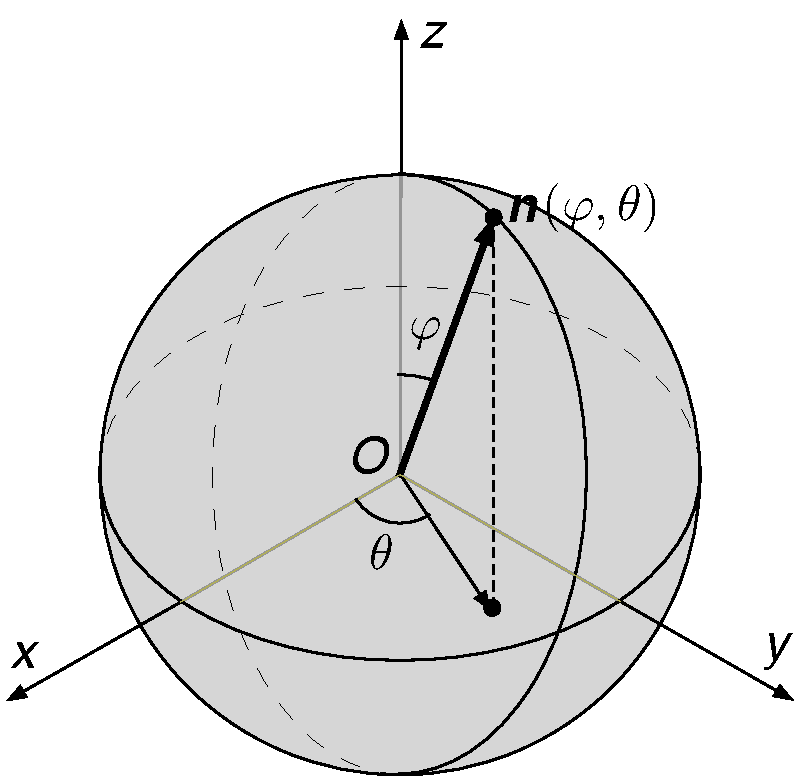
\includegraphics[width=67mm]{figs/spherical.pdf}
      \label{fig:spherical}
    }
    \subfigure[Stereographic]{
      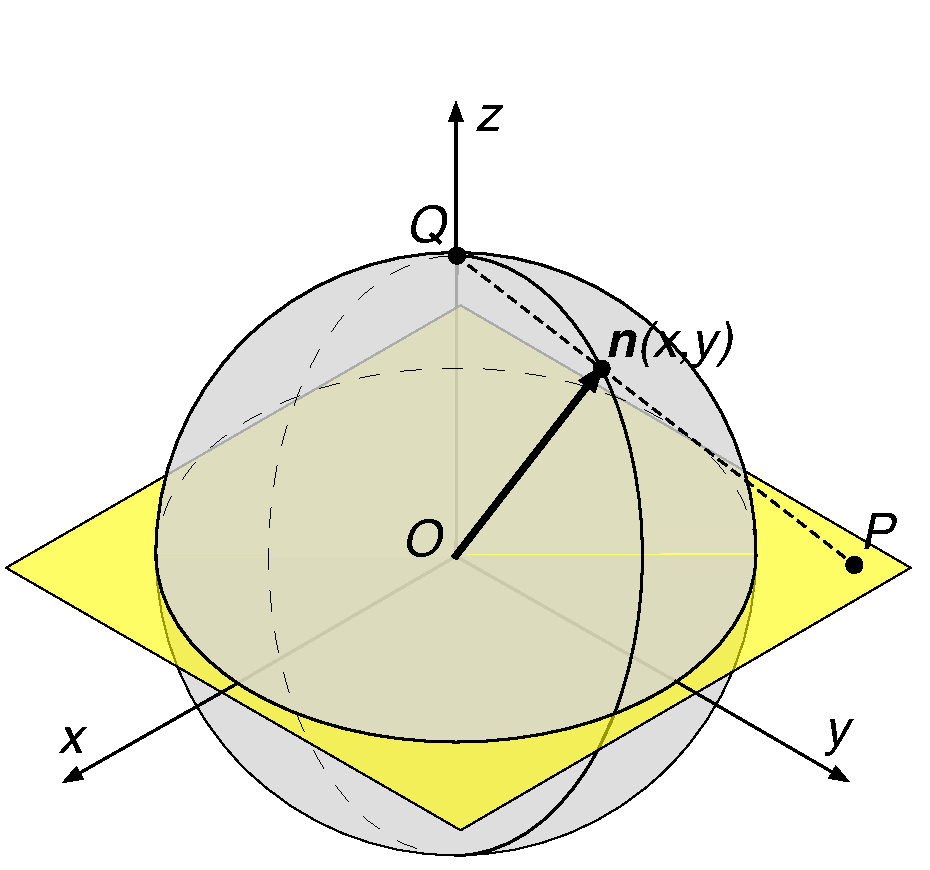
\includegraphics[width=67mm]{figs/stereographic.pdf}
      \label{fig:stereographic}
    }
    \subfigure[Projective]{
      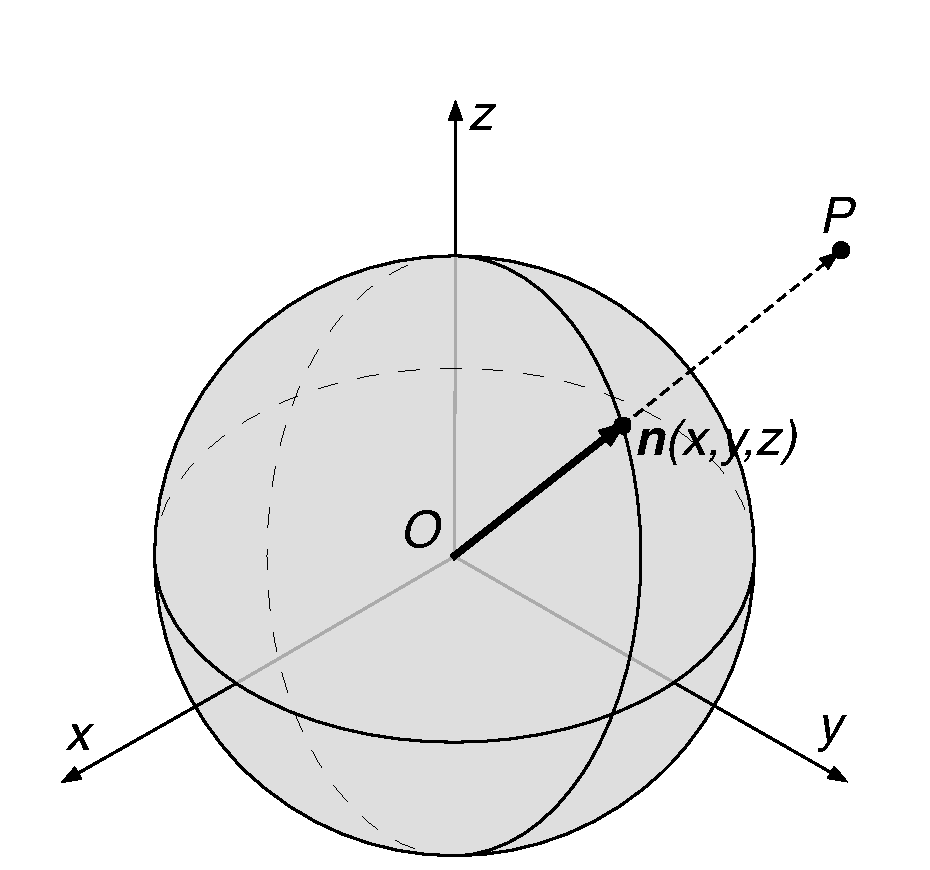
\includegraphics[width=67mm]{figs/projective.pdf}
      \label{fig:projective}
    }
    \subfigure[Tangent]{
      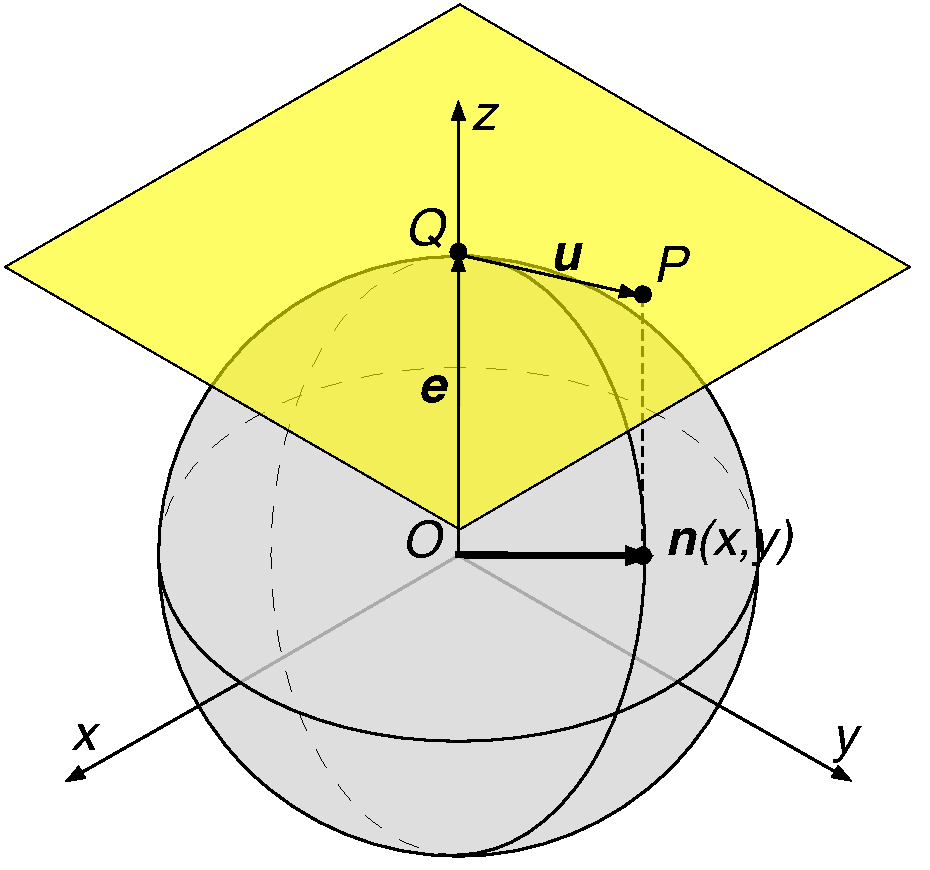
\includegraphics[width=67mm]{figs/tangent.pdf}
      \label{fig:tangent}
    }
    \subfigure[Cartesian]{
      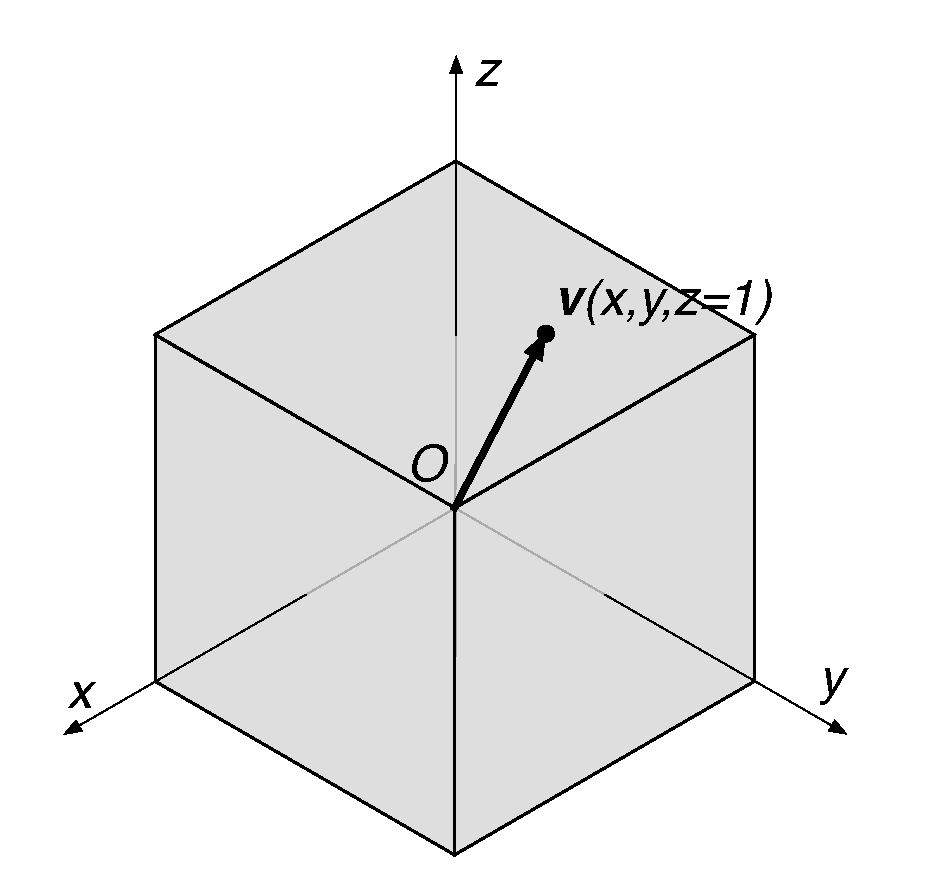
\includegraphics[width=67mm]{figs/cartesian.pdf}
      \label{fig:Cartesian}
    }
    \caption{Parametrizations.}
    \label{fig:parametrizations}
  \end{center}
\end{figure}

\section{Bifurcation Detection}
\label{sec:detection}

Within an incremental update setting, the numerical detection of the bifurcation condition for each time increment using any of the parametrizations just described consists of the following two steps:

\begin{itemize}
  
\item An initial sampling is performed over the 
parametric space for $\bq$ for the normal vector $\bn \in S^2$ or $\bv 
\in \bbR^3 \setminus \{\mathbf{0}\}$ associated with the 
parametrization. This leads to a rough estimate of minimum of the 
determinant function \eqref{eq:minimization-determinant} and the 
associated bifurcation directions.
  
\item The coarse estimate can be used to initiate an iterative 
procedure to find a more accurate estimate of the onset of bifurcation 
and its associated directions by solving the optimization problem in \eqref{eq:minimization-derivative}. 

\end{itemize}

In an actual finite element simulation, the above two-step procedure 
may not yield estimates of the bifurcation condition that are accurate 
enough due to finite time increment. One way to improve the solution 
is to introduce adaptive time increments. Define

\begin{equation} \label{eq:general-minimization-problem}
  \mu_n := \min_{\bq} f_n(\bq) = \min_{\bq} \det \bB_n(\bq)
\end{equation}

where the tensor $\bB_n(\bq)$ may be either the one from
\eref{eq:acoustic-tensor} or the one from
\eref{eq:Cartesian-acoustic-tensor}, depending on the parametrization
in use, and the index $n$ indicates that the evaluation occurs at time
$t_n$. 

Consider the original time increment from $t_n$ to $t_{n+1}$, where 
$\mu_n > 0$ and $\mu_{n+1} < 0$. This means that between time $t_n$ 
and $t_{n+1}$, the strong ellipticity condition is violated and hence 
material bifurcates. Assume also that $\mu_n / \mu_0 > \epsilon$, 
where $\mu_0$ is the value of the determinant function evaluated at 
time $t_0$ and $\epsilon$ is a target tolerance. We wish to find a 
better estimate for the determinant function $\mu_n$, and hence the 
bifurcation time $t_n$, such that $\mu_n / \mu_0 \le \epsilon$. This 
is achieved by an adaptive time increment procedure by means of 
bisection, as shown in Algorithm~\ref{alg:adaptive-step}. This 
algorithm repeatedly cut the time increment to half until the 
convergence criteria $\mu_n / \mu_0 \le \epsilon$ is met.

\begin{algorithm}
  \caption{$\text{AdaptiveStep}(\mu_0, \mu_{n+1}, t_{n+1}, \epsilon)$}
  \begin{algorithmic}
    \REQUIRE $\mu_{n+1} < 0$
    \ENSURE $\mu_{n+1,k} \in [0, \epsilon \mu_0]$
    \STATE initialize
    $k \leftarrow 1,
    \quad
    \alpha \leftarrow \frac{1}{2},
    \quad
    \triangle t \leftarrow t_{n+1} - t_n,
    \quad
    \mu_{n+1,k} \leftarrow \mu_{n+1}$
    \WHILE{ $\mu_{n+1,k} < 0$ {  or  } $ \mu_{n+1,k} / \mu_0
      > \epsilon$ }
    \STATE $t_{n+1,k} \leftarrow t_n + \alpha \triangle t$
    \STATE compute $\bF(t_{n+1,k})$ using the global solution scheme
    \STATE compute $\triangle \bZ(t_{n+1,k})$
    by solving \eref{eq:Biots-equation-discrete}
    \STATE compute $\bbC(t_{n+1,k})$
    using \eref{eq:incremental-stress-moduli}
    \STATE compute $\mu_{n+1,k}$
    by solving \eref{eq:general-minimization-problem}
    \IF{$\mu_{n+1,k} > 0$}
    \STATE $\alpha \leftarrow \alpha + 2^{-k}$
    \ELSE
    \STATE $\alpha \leftarrow \alpha - 2^{-k}$
    \ENDIF
    \STATE $k \leftarrow k+1$
    \ENDWHILE
  \end{algorithmic}
  \label{alg:adaptive-step}
\end{algorithm}

The adaptive time increment procedure allows the accurate (up to the
tolerance $\epsilon$) detection of bifurcation time during a loading
process. The procedure described in this section to numerically detect 
material bifurcation can be applied to a very general class of 
materials and will be analyzed in the following section.

\section{Numerical Examples}
\label{sec:numerical-examples}

The performance and applicability of the proposed Cartesian along with 
other existing common and uncommon parametrizations are examined by 
applying them to the bifurcation analysis of several material models 
under different loading conditions. The analysis is performed at the 
material point level. Of particular interest are the robustness and 
computational efficiency of different parametrizations.

\subsection{Small deformation isotropic elastic damage model}
\label{subsec:isotropic}

We start the bifurcation analysis on a simple small deformation 
isotropic damage model. The model formulation is briefly presented 
first. Then, a simple shear test will be performed to study the 
performance of different parametrizations on the detection of material 
bifurcation.

\subsubsection{Model formulation}

The stress and constitutive tangent of the small deformation isotropic 
damage model will be derived from a strain-energy function, which is 
assumed to have the following form:

\begin{equation}\label{eq:iso_psi}
 \Psi(\bepsilon ^e, \xi)
   = \frac{1}{2} (1 - \xi) 
     \bepsilon ^e : \mathbb{C}^e : \bepsilon ^e
\end{equation}

where $\bepsilon^e$ is the infinitesimal elastic strain tensor, 
$\mathbb{C}^e$ is the fourth-order elastic modulus, and $\xi$ 
is a damage parameter introduced to trigger material bifurcation. For 
isotropic linear elasticity, the elastic modulus $\mathbb{C}^e$ is 
given as

\begin{equation}
  \mathbb{C}^e = \lambda \bdelta\otimes\delta + 2\mu\bI
\end{equation}

where $\lambda$ and $\mu$ are Lam\'{e} constant and shear modulus,
respectively. $\bdelta$ is the second-order identity tensor,
$(\bI)_{ijkl} = 1/2(\delta_{ik}\delta_{jl} +
\delta_{il}\delta_{jk})$ is the fourth-order symmetric identity
tensor.

We adopt the following evolution law for the scalar damage parameter $
\xi$ \cite{Holzapfel:2000}

\begin{equation}\label{eq:iso_xi}
  \xi(\alpha) = \xi_{\infty} [ 1- {\rm exp}(-\alpha / \tau)]
\end{equation}

where $\xi_{\infty}$ describes the dimensionless maximum damage and
$\tau$ is referred to as the damage saturation parameter. The 
parameter $\alpha$ is the maximum thermodynamic force 
\cite{Holzapfel:2000} with the same dimension as the effective strain 
energy. Within the closed time interval $[0,t]$, $\alpha$ is given as

\begin{equation}\label{eq:alpha}
  \alpha(t) = \max_{s\in [0,t]}\Psi_0(s)
\end{equation}

where $\Psi_0(s)$ is the undamaged strain energy at time $s$.
$s \in [0,t]$ denotes the history variable.

Given the strain-energy function \eref{eq:iso_psi} and the damage
evolution \eref{eq:iso_xi}, the fourth-order tangent modulus can be
derived by taking 2nd derivative of the strain-energy function with
respect to the strain measure $\bepsilon_e$, which results in

\begin{equation}
  \mathbb{C} = (1-\xi)\mathbb{C}^e 
    - \beta \frac{\partial\xi}{\partial\alpha}
    (\bsigma_0\otimes\bsigma_0)
\end{equation}

where $\bsigma_0$ is the effective (undamaged) Cauchy stress. 
$\beta = 1$ if damage evolves within the time increment and $\beta=0$ 
otherwise. This tangent modulus will be used to compute the acoustic 
tensor \eref{eq:acoustic-tensor}, which will then be checked for 
material bifurcation.

\subsubsection{Simple shear test}

In this section, a simple shear test is simulated, where the following 
material properties are used: $\lambda = 80$, $\mu = 80$, 
$\xi_{\infty} = 1.0$ and $\tau = 1.0$. The resulting shear stress vs. 
shear strain is plotted in Figure~\ref{fig:iso_stress_strain}(a). The 
softening response is due to the evolution of the introduced damage 
parameter $\xi$. 

For the numerical detection of material bifurcation, the two-step 
procedure described in Section \ref{sec:detection} is adopted, i.e., 
(1) an initial sampling performed over the parametric space, and (2) a 
Newton iterative procedure for better estimate of the onset of  
bifurcation and its associated directions. Figure~
\ref{fig:iso_stress_strain}(b) shows the degradation of the 
determinant function (det$\bA$) for all five parametrizations upto the 
point material bifurcation is detected. When det$\bA = 0$, the 
material bifurcates. In this example, all five parametrizations detect 
bifurcation at the same time, i.e., when the shear strain 
$\epsilon_{12}=0.0559$ as marked in Figure~
\ref{fig:iso_stress_strain} (a). With the adaptive time step 
algorithm, the precise time (upto the set tolerance) of bifurcation 
can be detected.

\begin{figure}[H]
  \centering \subfigure[]{
    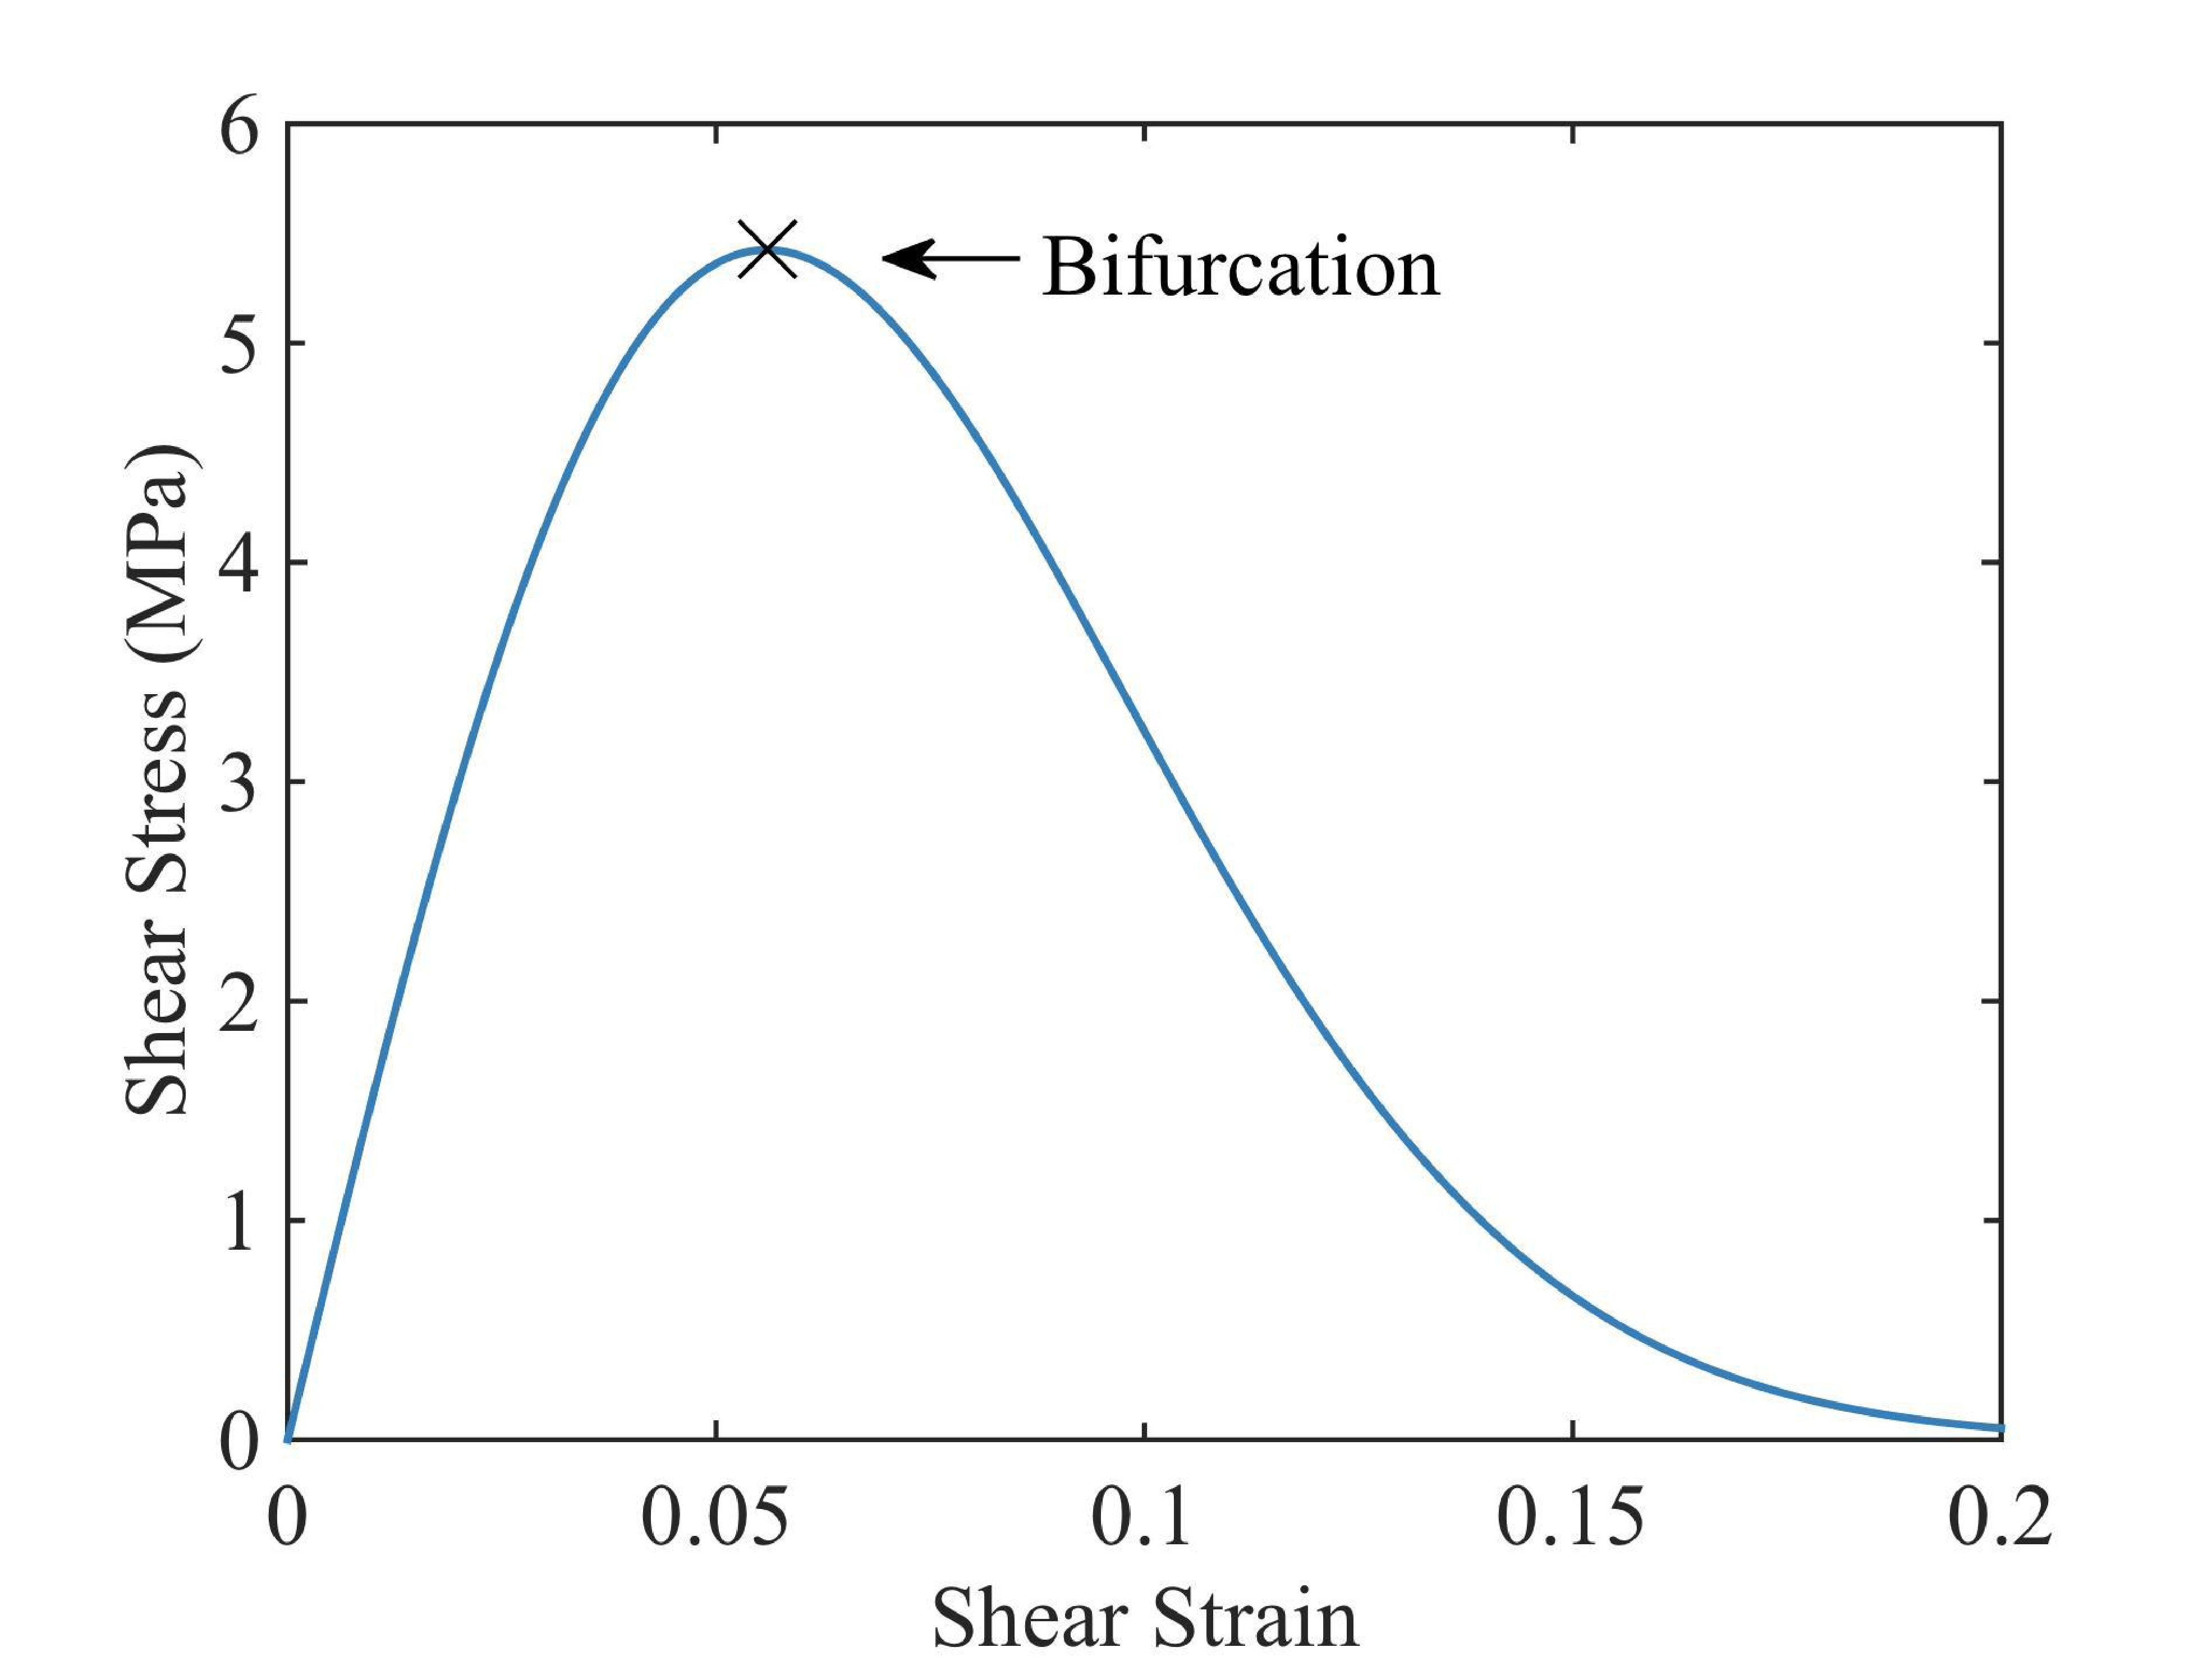
\includegraphics[width=0.45\textwidth]
    {figs/iso_shear_stress_strain.pdf}
  } \subfigure[]{
    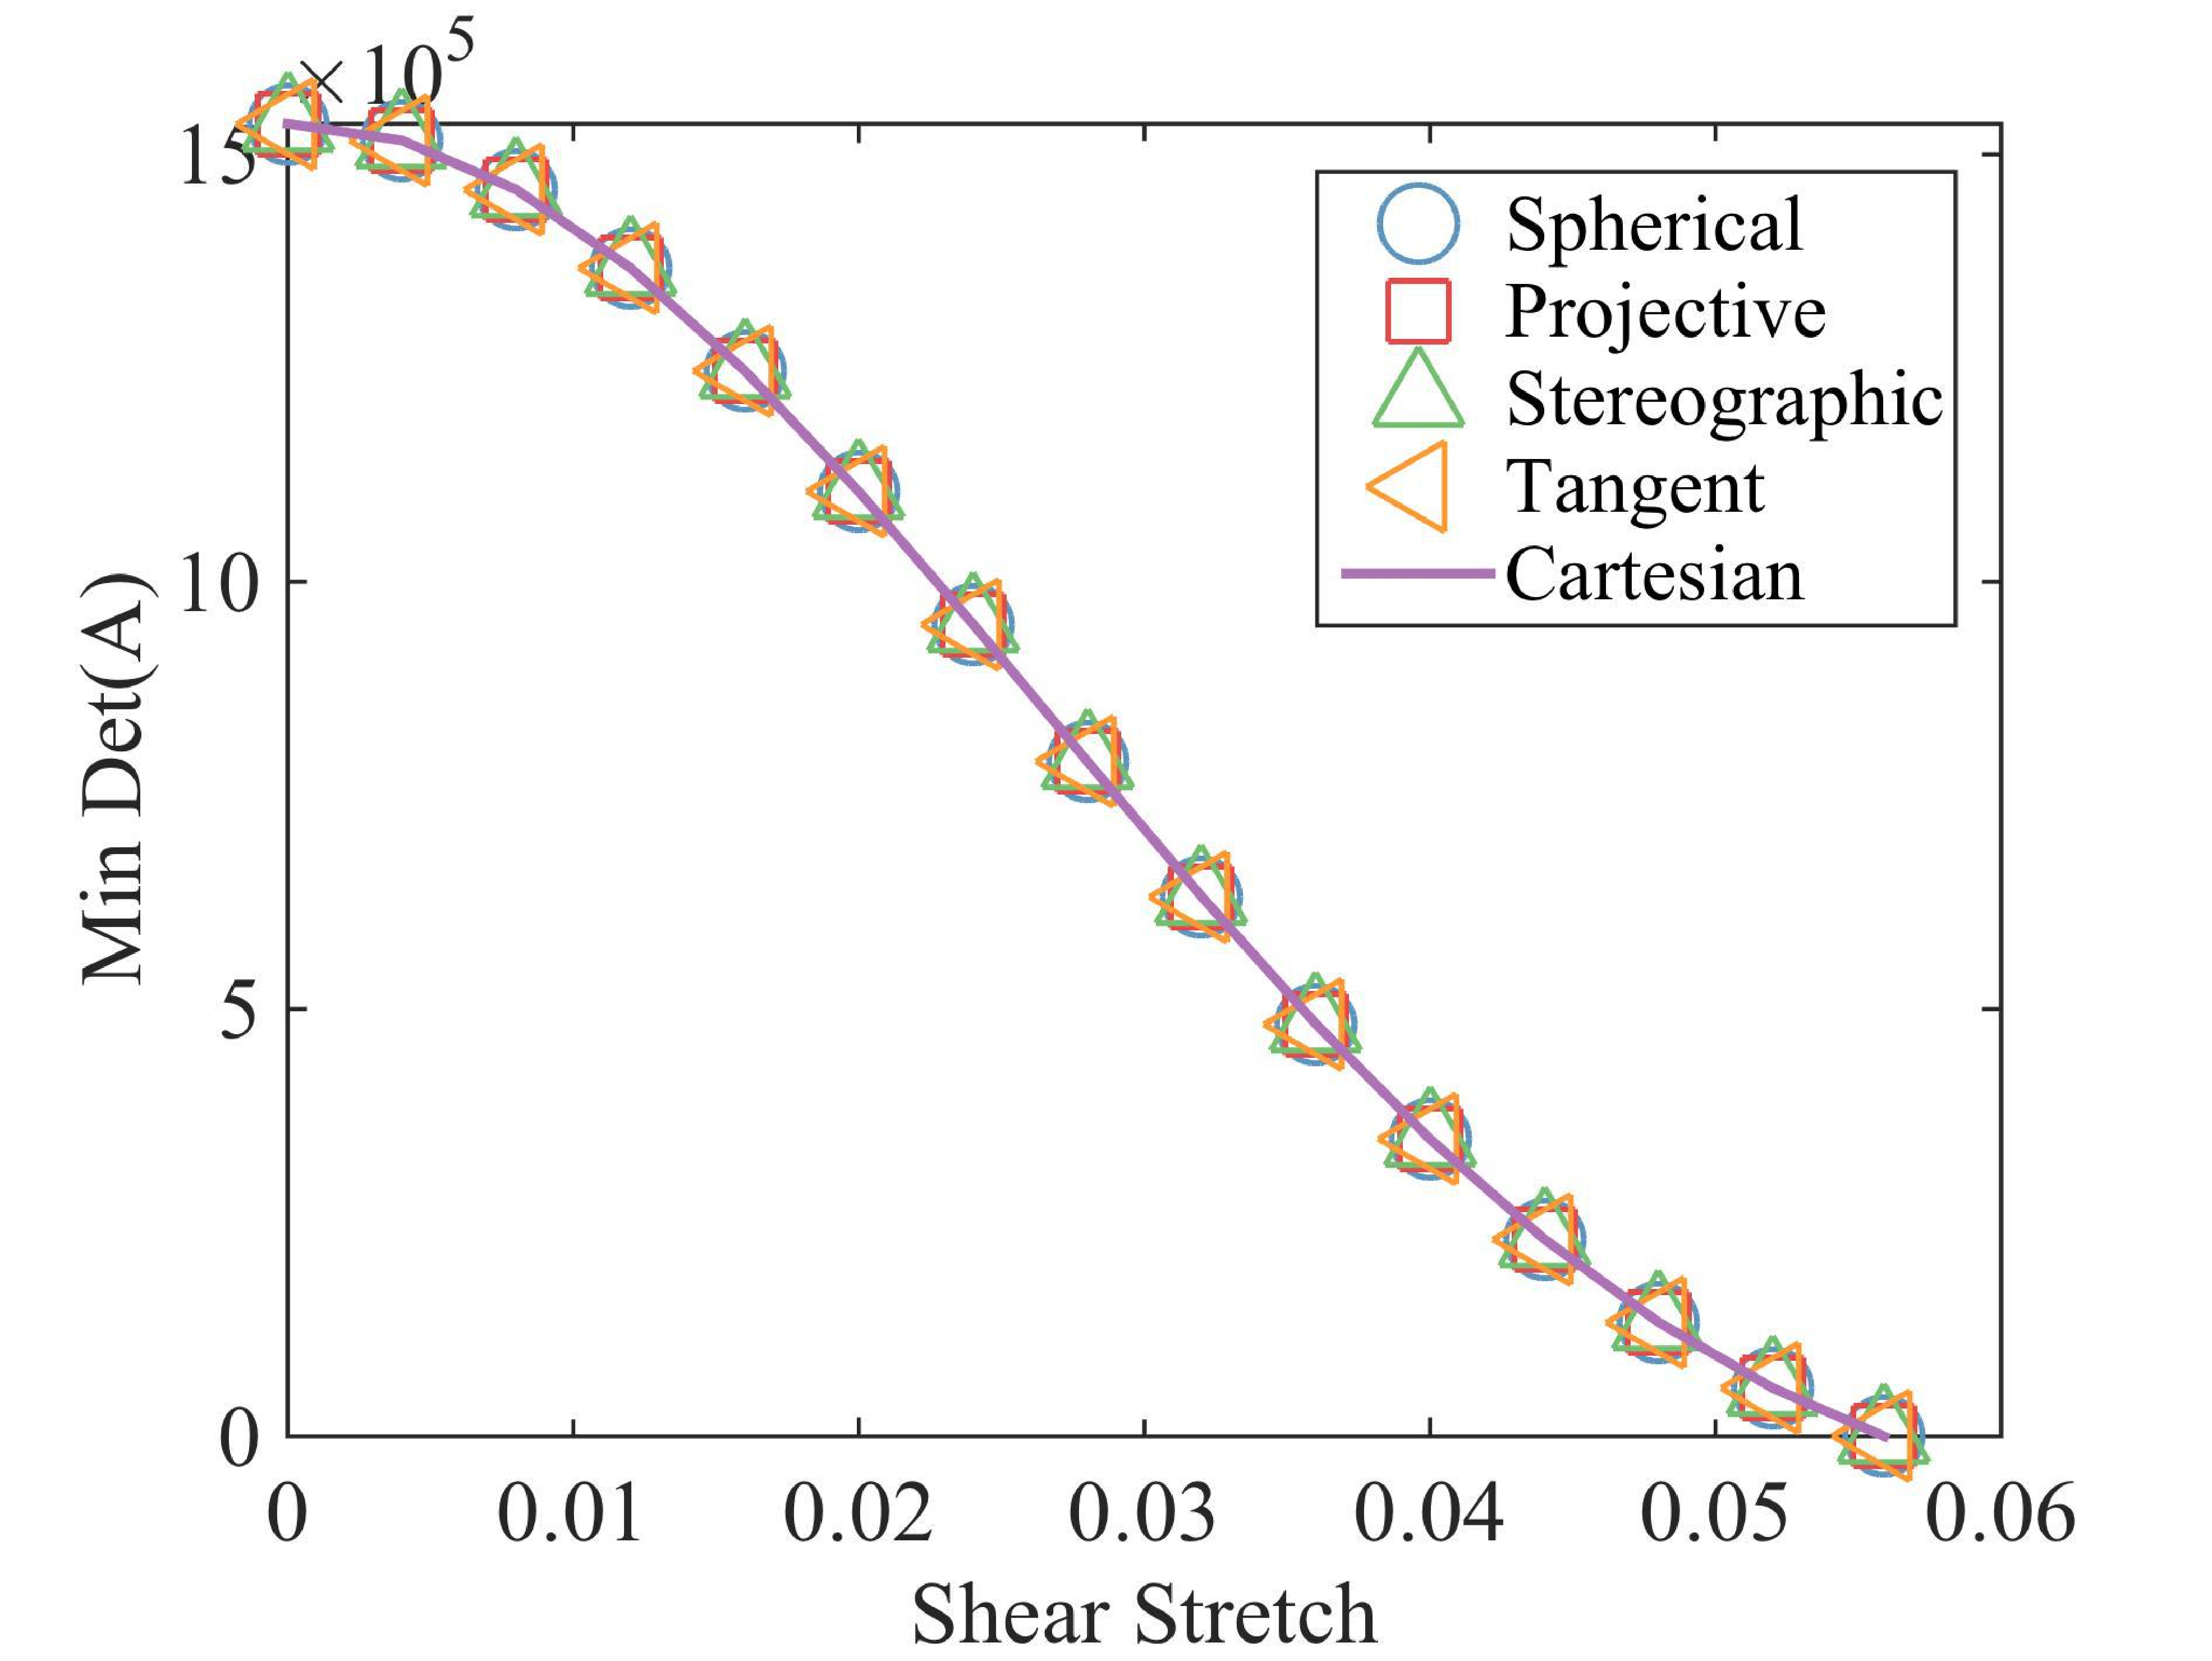
\includegraphics[width=0.45\textwidth]
    {figs/iso_shear_mindetA_strain.pdf}
  }
  \caption{Simple shear test on small deformation 
  isotropic damage model: 
  (a)stress strain behavior, with the cross indicating bifurcation, and
  (b) degradation of det$\bA$ for different
  parametrizations upto the point material bifurcation is detected ($\epsilon_{12}=0.0559$).}
  \label{fig:iso_stress_strain}
\end{figure}

While all five parametrizations detect bifurcation at the same time, 
Figure~\ref{fig:iso_stress_strain}(b) provides little information on 
their computational efficiency and robustness, which are the focus of 
this work. The computational cost of bifurcation detection mainly 
consists of two parts: (1) the time for the initial sampling over the 
parametric space, and (2) the time for the Newton iterative solve. 

The time for the initial sampling depends on the number of sampling 
points, or equivalently, the density of the initial sampling grid. The 
denser the initial sampling grid is, the more expensive it is 
computationally to perform the sweep. The time for the Newton 
iterative solve, on the other hand, depends mainly on the complexity 
of the objective function, i.e., det$\bA$, as well as the quality of 
the initial guess.

To compare computational costs of different parametrizations, we 
record the time spent on bifurcation check at a particular loading 
increment, e.g., at the increment leading to bifurcation. We also vary 
the density of the initial sampling grid to study its effect on 
different parametrizations. A robust parametrization should be 
insensitive to the initial sampling grids.

The results on computational cost are summarized in Table~
\ref{tab:iso_shear_runtime}. The density of the initial sampling grid 
is represented by the sampling interval and the number of sampling 
points. The table only shows the number of sampling points, $N$, along 
one dimension of the parametric space. The total number of sampling 
points should be $N^{dim}$, where $dim$ is the total dimension of 
the parametric space. For instance, for spherical parametrization, 
there are two independent parameters, $\varphi$ and $\theta$. 
Therefore, $dim=2$ for spherical parametrization.

It can be seen from Table~\ref{tab:iso_shear_runtime}, as the number 
of sampling points $N$ per dimension decreases, so does the 
computational cost. The spherical and the Cartesian parametrizations 
are the most efficient. The stereographic, projective and tangent are 
more computationally expensive. In the extreme case with $N=1$, 
meaning there is only one initial sampling point per dimension, the 
stereographic, projective and tangent fail to correctly detect 
bifurcation, shown as `n/a' in the table. 

\begin{table}[H]
  \begin{center}
    %\begin{tabular}{ p{1.5cm} | p{1.7cm} p{1.7cm} p{1.7cm} p{1.7cm} p{1.7cm} }
    \begin{tabular}{c c | r r r r r}
      \toprule
      Sampling   & Sampling &   \multicolumn{5}{c}{Run time ($\mu$s)}	\\   
      interval     & points ($N$)     &  Spherical    &   Stereographic  &   Projective  &   Tangent   & Cartesian  \\
      \midrule         
      0.05      &      41     &    305        &       155       &       5636      &      226       &       347         \\
      0.1        &      21     &    125        &       89         &       884        &      107       &       115         \\
      0.2        &      11     &    85          &       60         &       183        &      64         &       81         \\
      0.3        &      7       &    60          &       184       &       178        &      157       &       39          \\
      0.4        &      5       &    74          &       181       &       197        &      145       &       27          \\       
      0.5        &	    5       &    74          &       37         &       88          &      53         &       27          \\
      0.6        &	    3       &    72          &       174       &       200        &      215       &       23          \\
      0.7        &	    3       &    71	      &       180       &       188        &      188       &       23          \\
      0.8        &      3       &    54          &       170       &       188        &      144       &       24          \\	      
      0.9        &	    3       &    53          &       177       &       156        &      159       &       23          \\	
      1.0        &      3	     &    43	      &       37         &       79          &      51         &       23          \\	
      1.5        &	    1       &    52	      &       n/a        &       n/a         &      n/a        &       21          \\	       
      \bottomrule
    \end{tabular}
    \caption{Computational cost of different parametrizations in 
    simple shear test at loading increment leading to bifurcation. 
    `n/a' means the parametrization fails to detect bifurcation in 
    this loading increment.}
    \label{tab:iso_shear_runtime}
  \end{center}
\end{table}

As aforementioned, the choice of parametrization directly affects the 
complexity of the objective function ${\rm det}\bA$ in 
\eref{eq:minimization-derivative}, which in turn affects the 
computational efficiency and robustness of different parametrizations 
on detection of material bifurcation as shown in 
Table~\ref{tab:iso_shear_runtime}. To illustrate this point, the 
landscapes of the objective function ${\rm det}\bA$ at bifurcation, 
i.e., at $\bepsilon_{12}=0.0559$ are plotted in 
Figure~\ref{fig:iso_shear_detA}. The corresponding plane views of the 
determinant landscapes are shown in 
Figure~\ref{fig:iso_shear_detAXplane}, where the white stars indicate 
global minimum point(s). The projective parametrization requires three parameters and is not visualized in this work.

\begin{figure}[H]
   \centering \subfigure[Spherical]{
   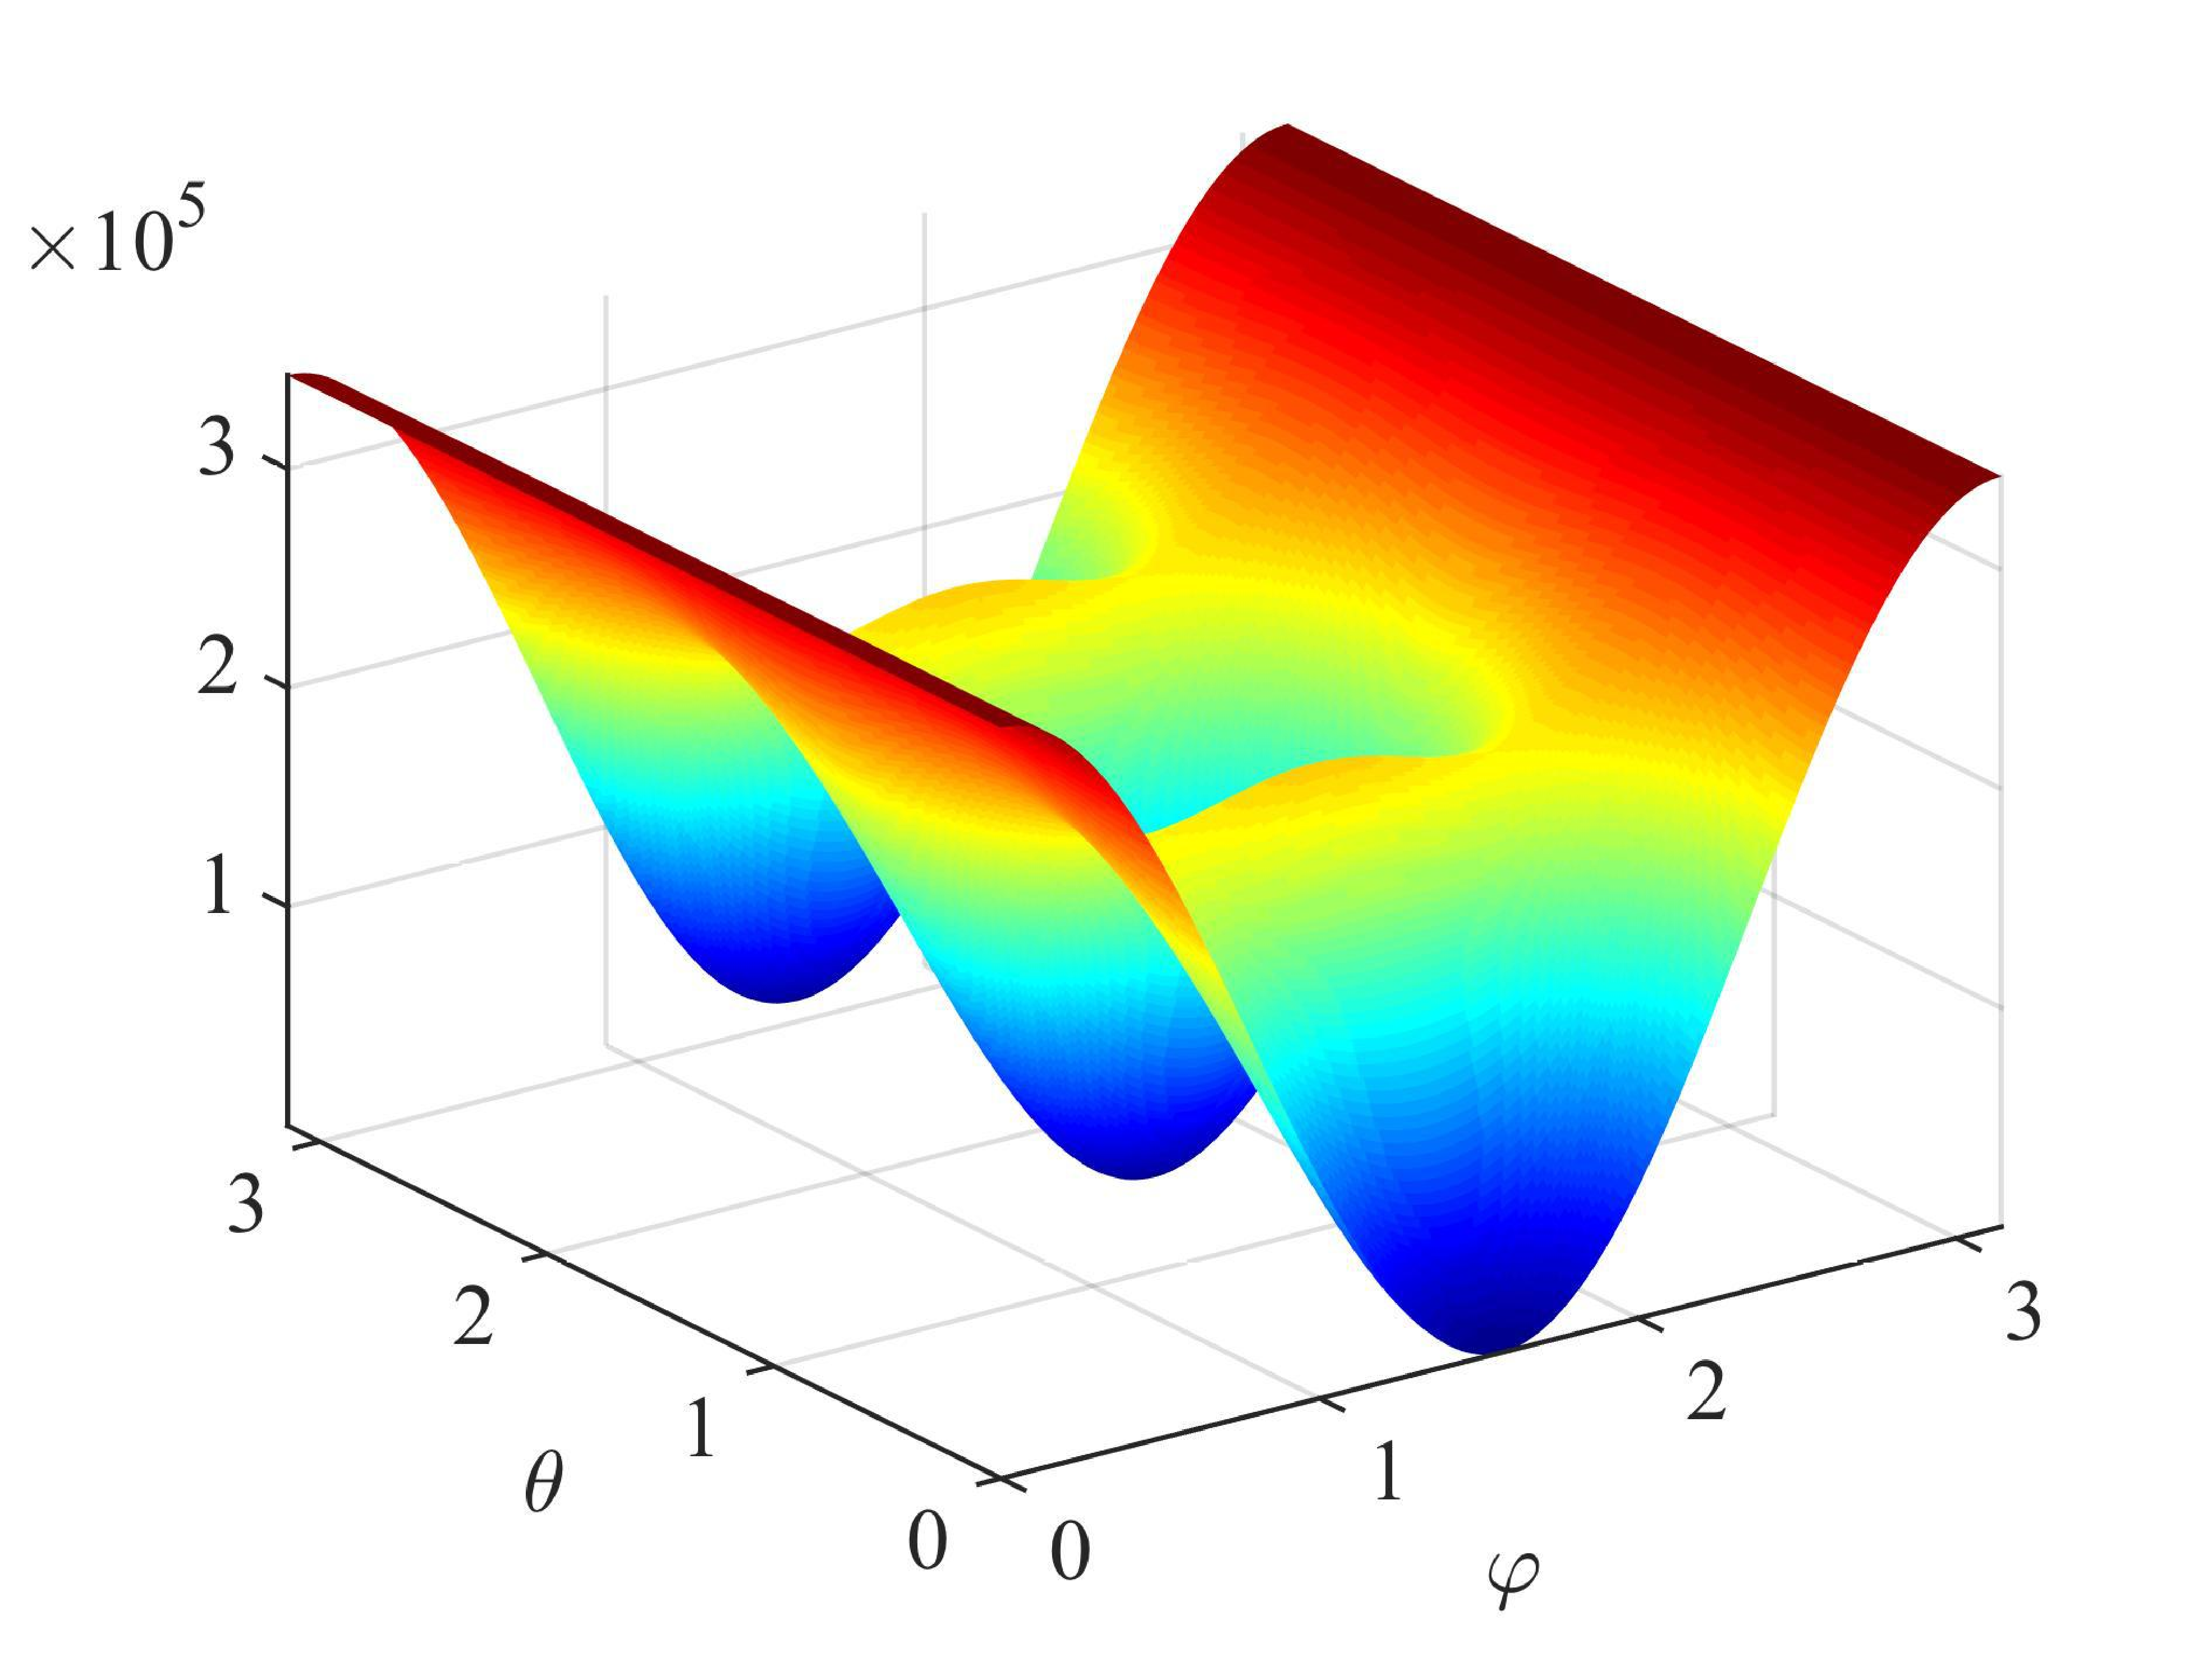
\includegraphics[width=0.45\textwidth]
   {figs/iso_shear_spherical_detA.pdf}
 } \subfigure[Cartesian]{
   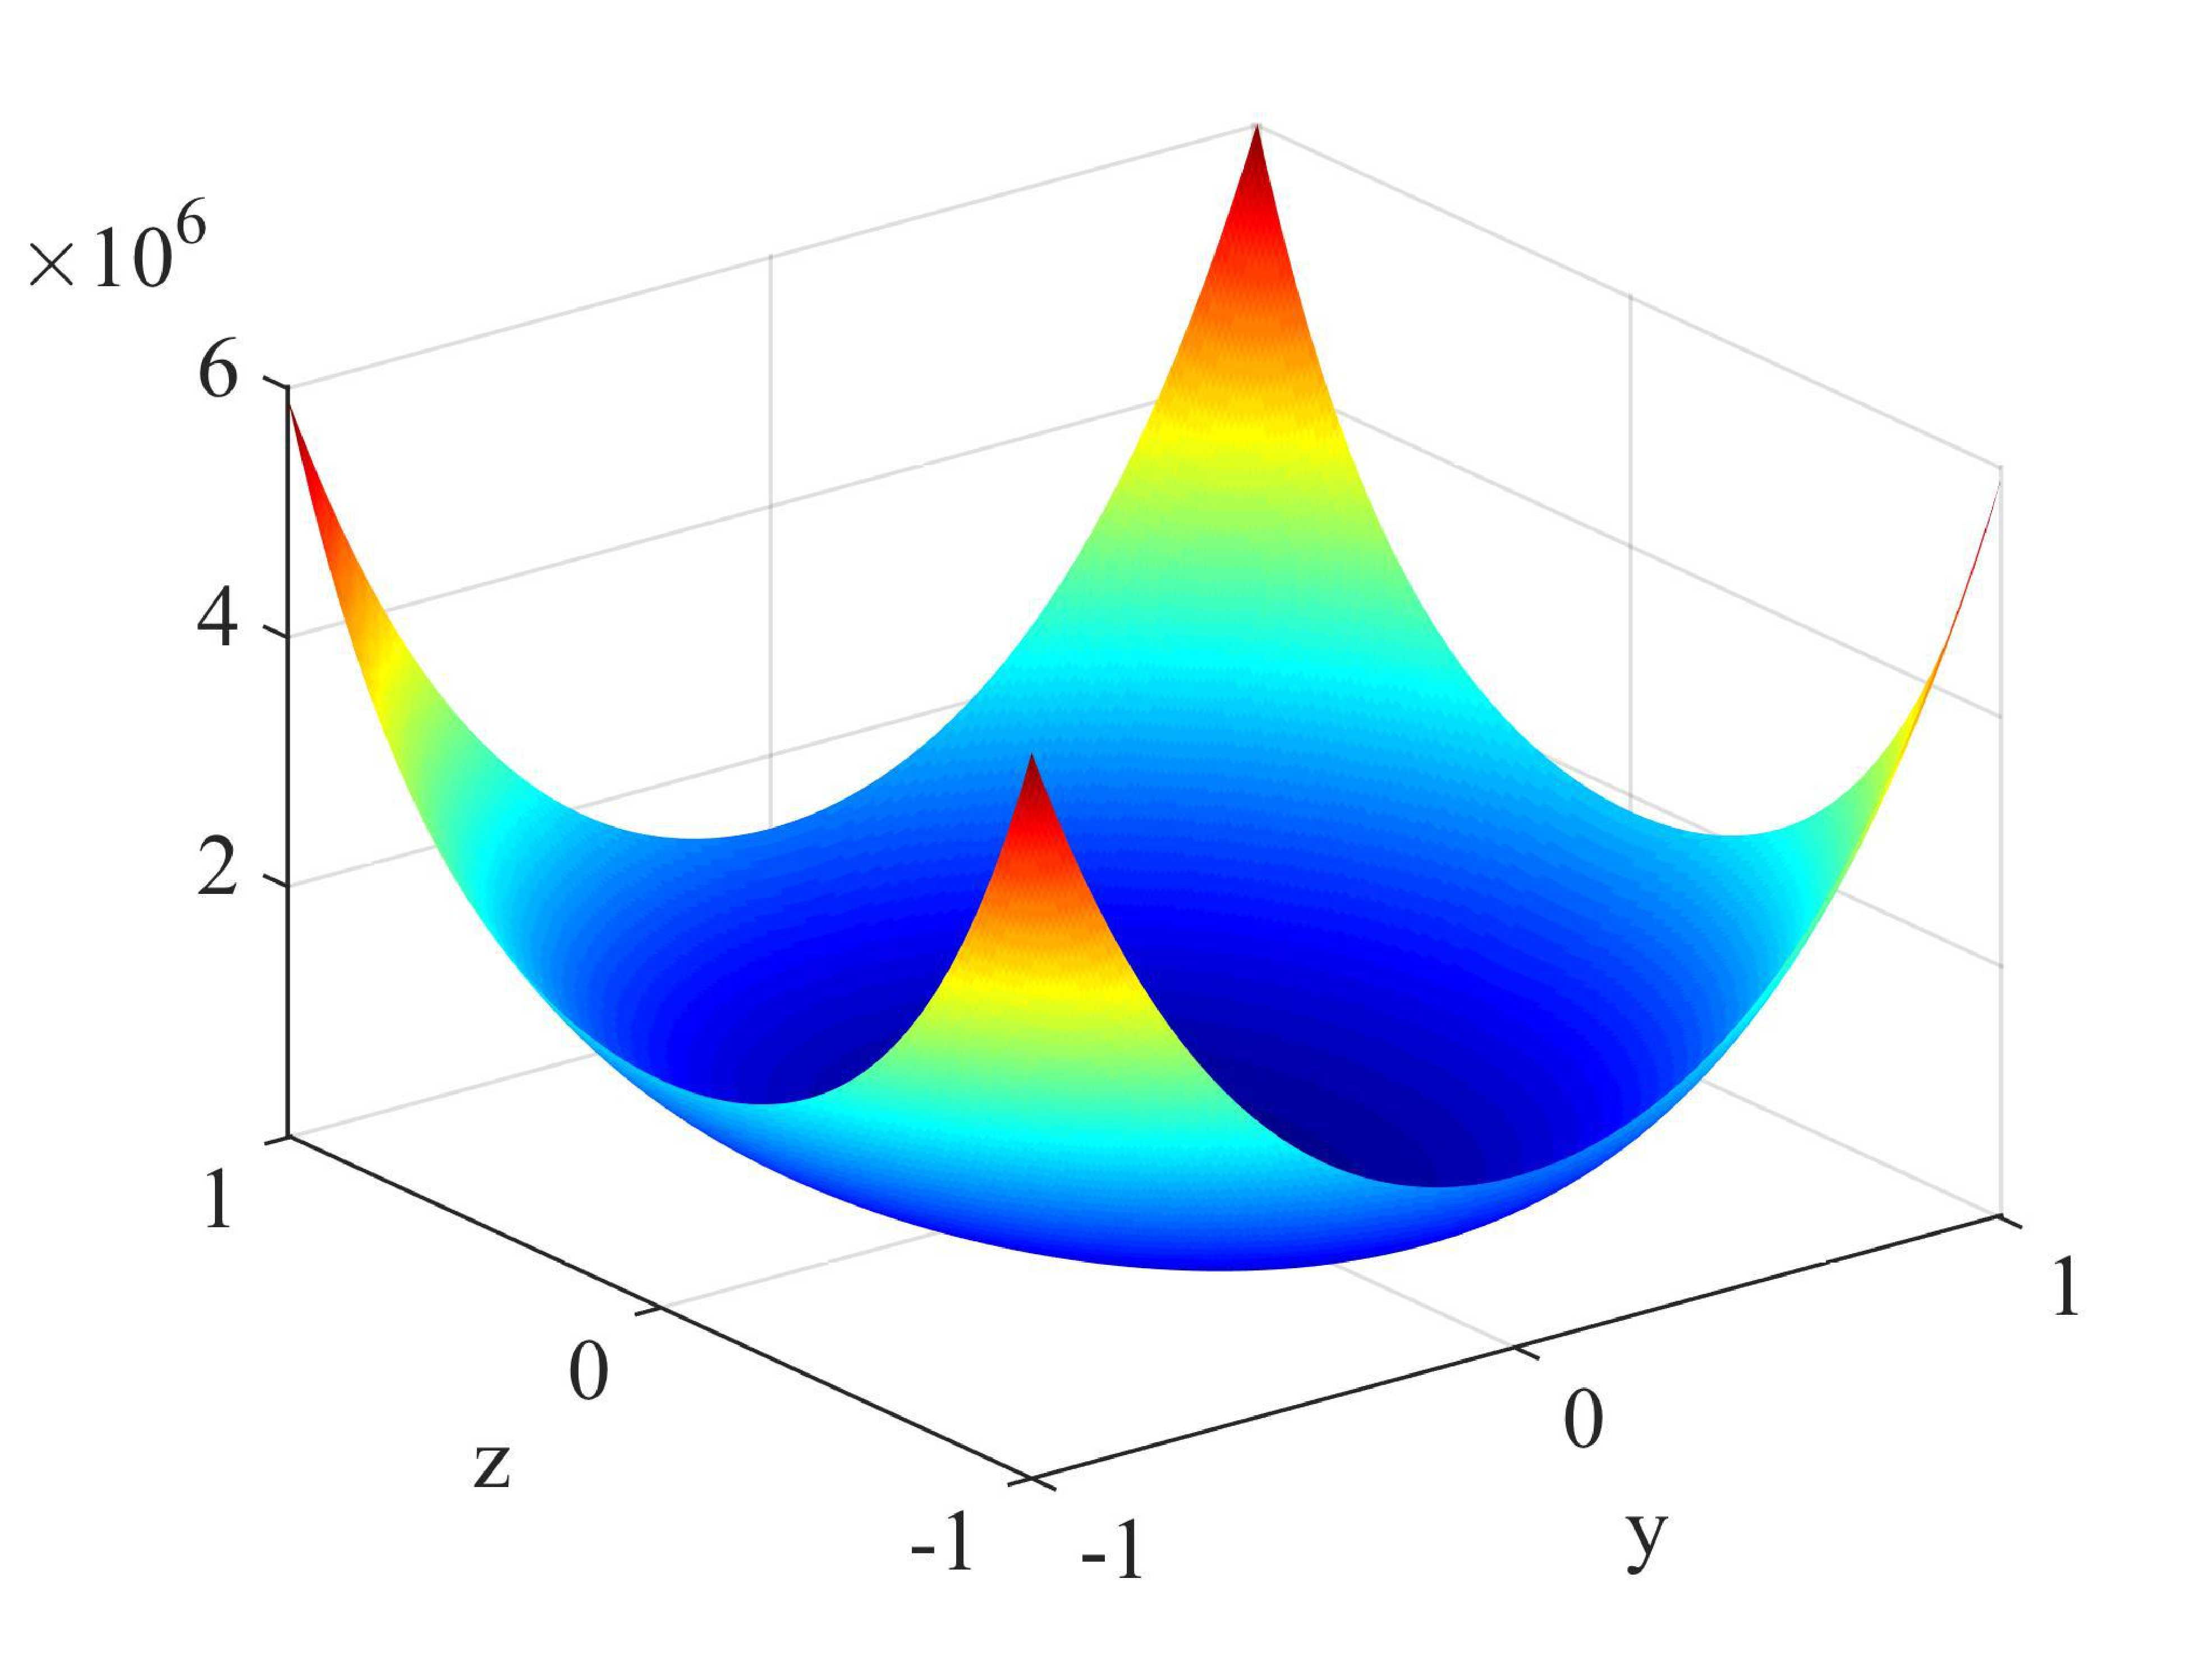
\includegraphics[width=0.45\textwidth]
   {figs/iso_shear_cartesian_detA.pdf}
 } \subfigure[Stereographic]{
   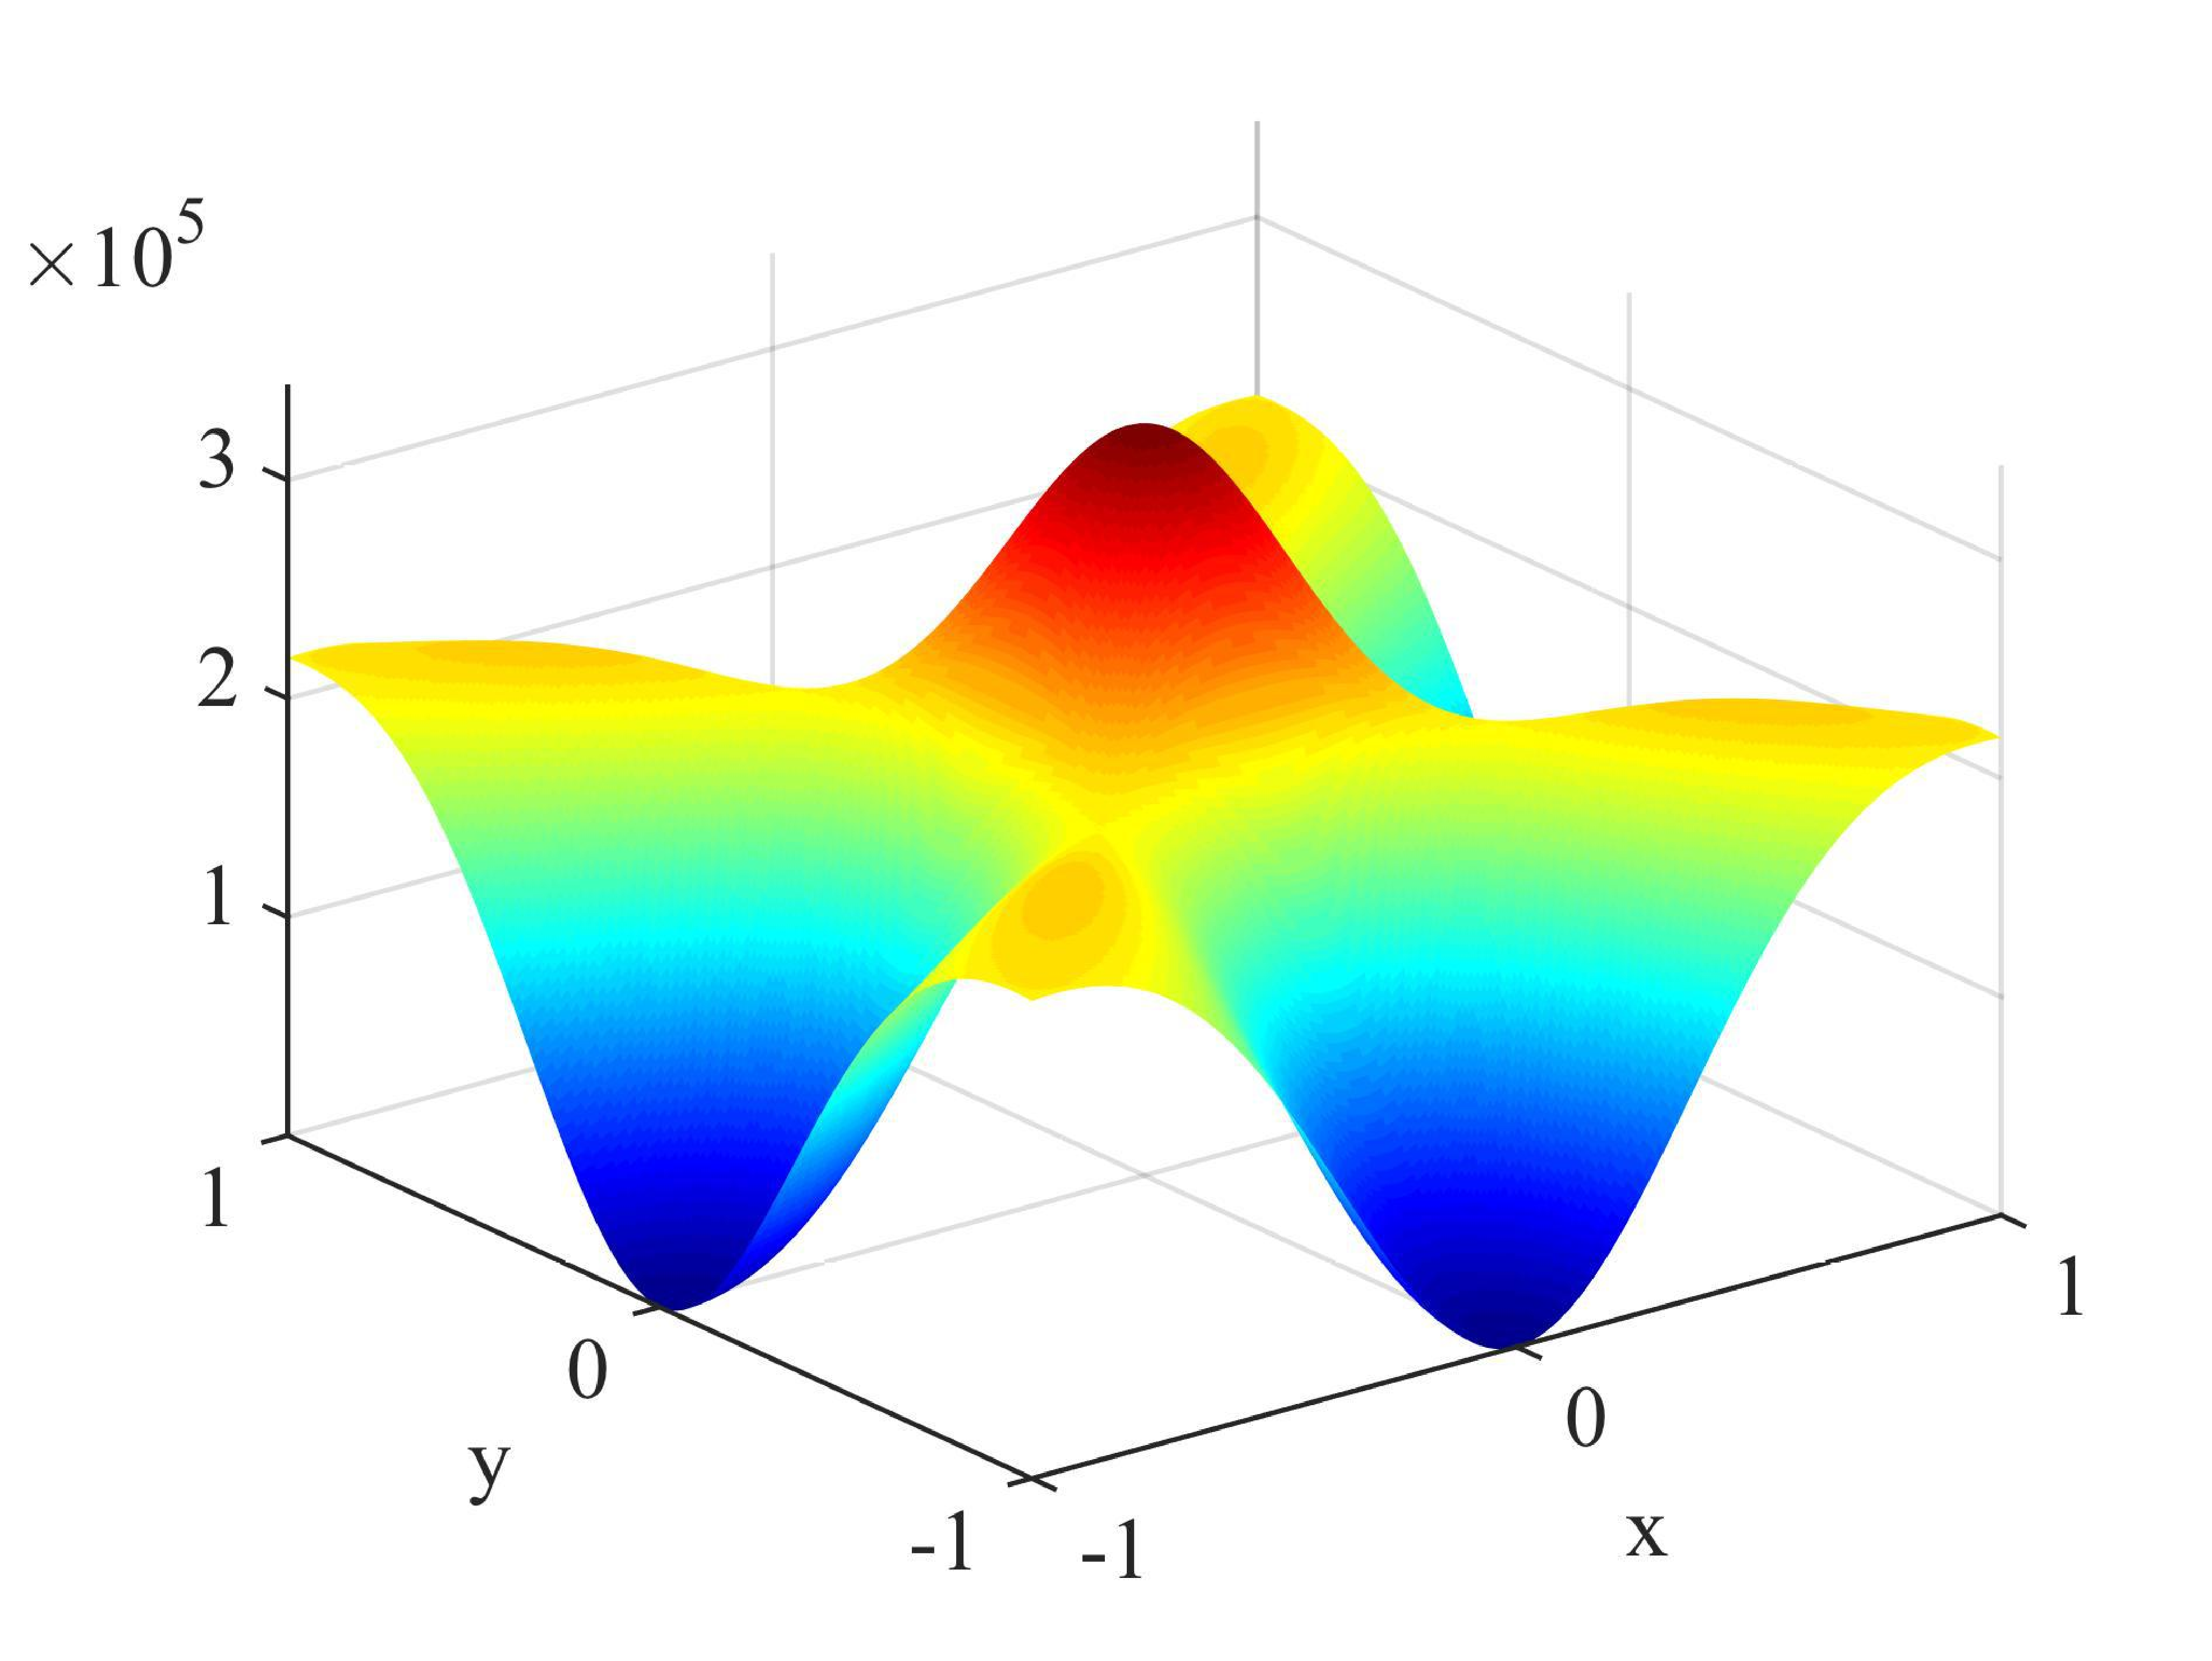
\includegraphics[width=0.45\textwidth]
   {figs/iso_shear_stereographic_detA.pdf}
 } \subfigure[Tangent]{
   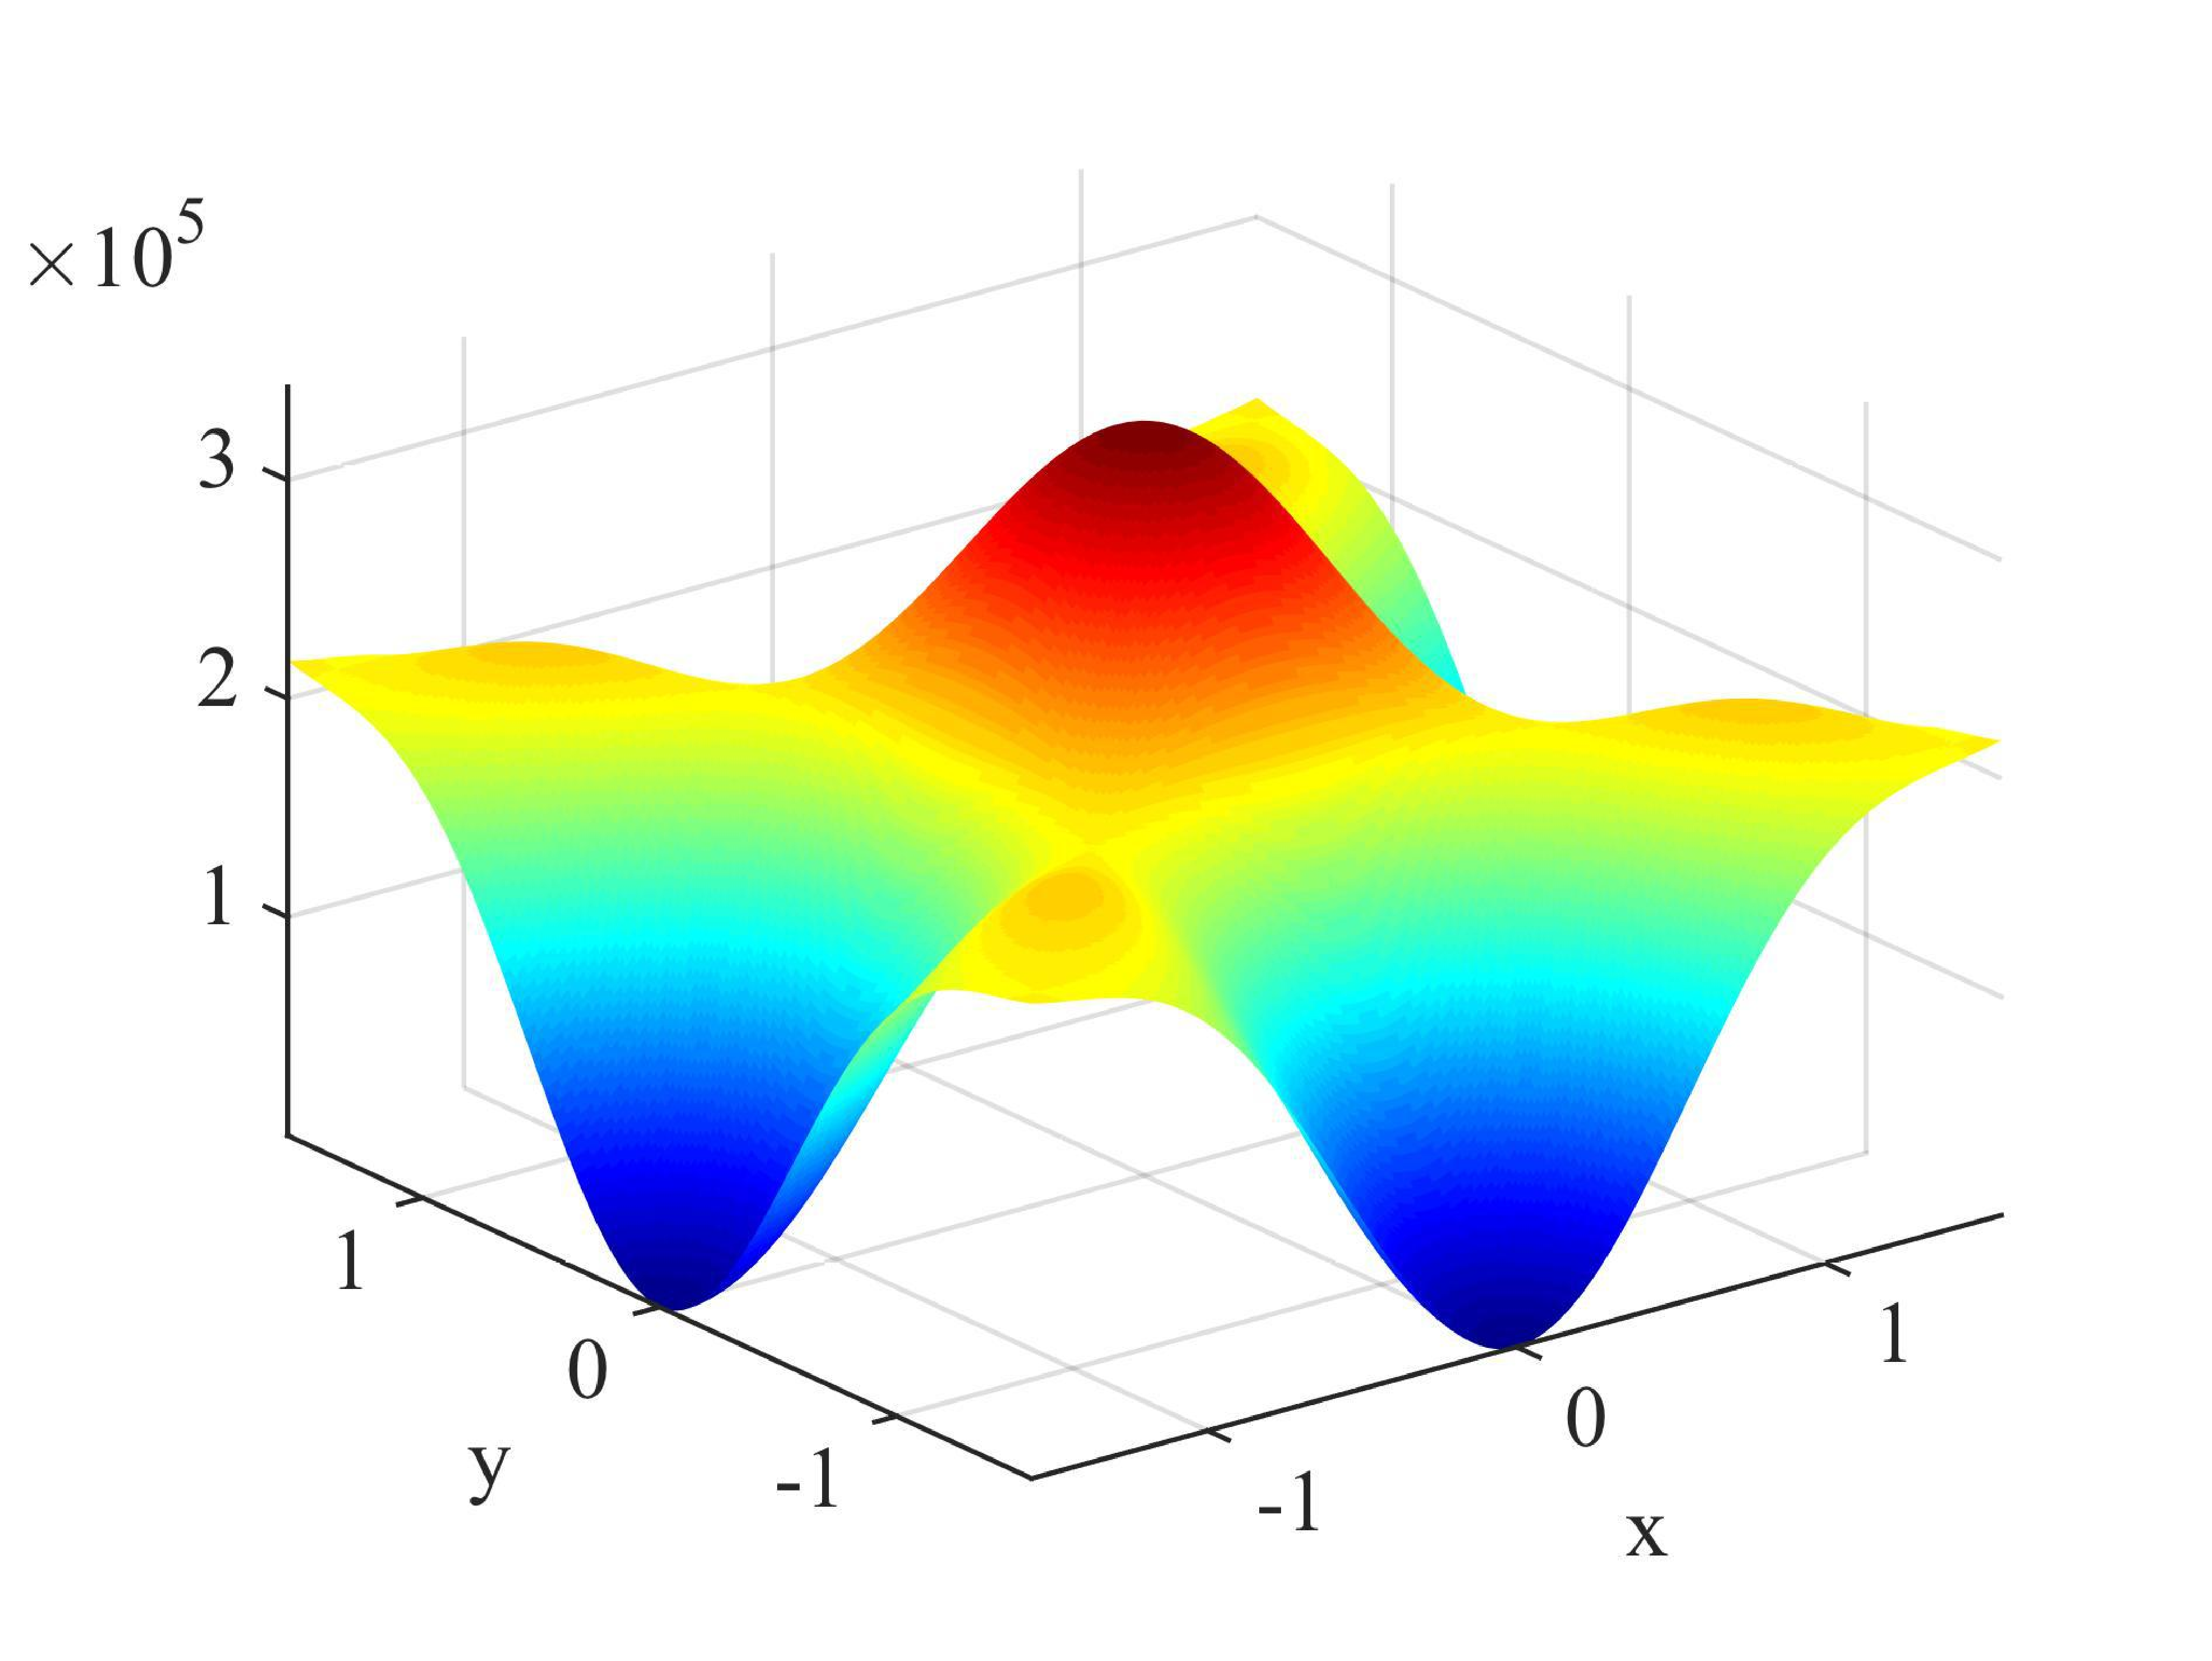
\includegraphics[width=0.45\textwidth]
   {figs/iso_shear_tangent_detA.pdf}
 }
   \caption{det$\bA$ landscapes at bifurcation
   for simple shear test on small deformation isotropic damage model.}
   \label{fig:iso_shear_detA}
 \end{figure}

\begin{figure}[H]
   \centering \subfigure[Spherical]{
   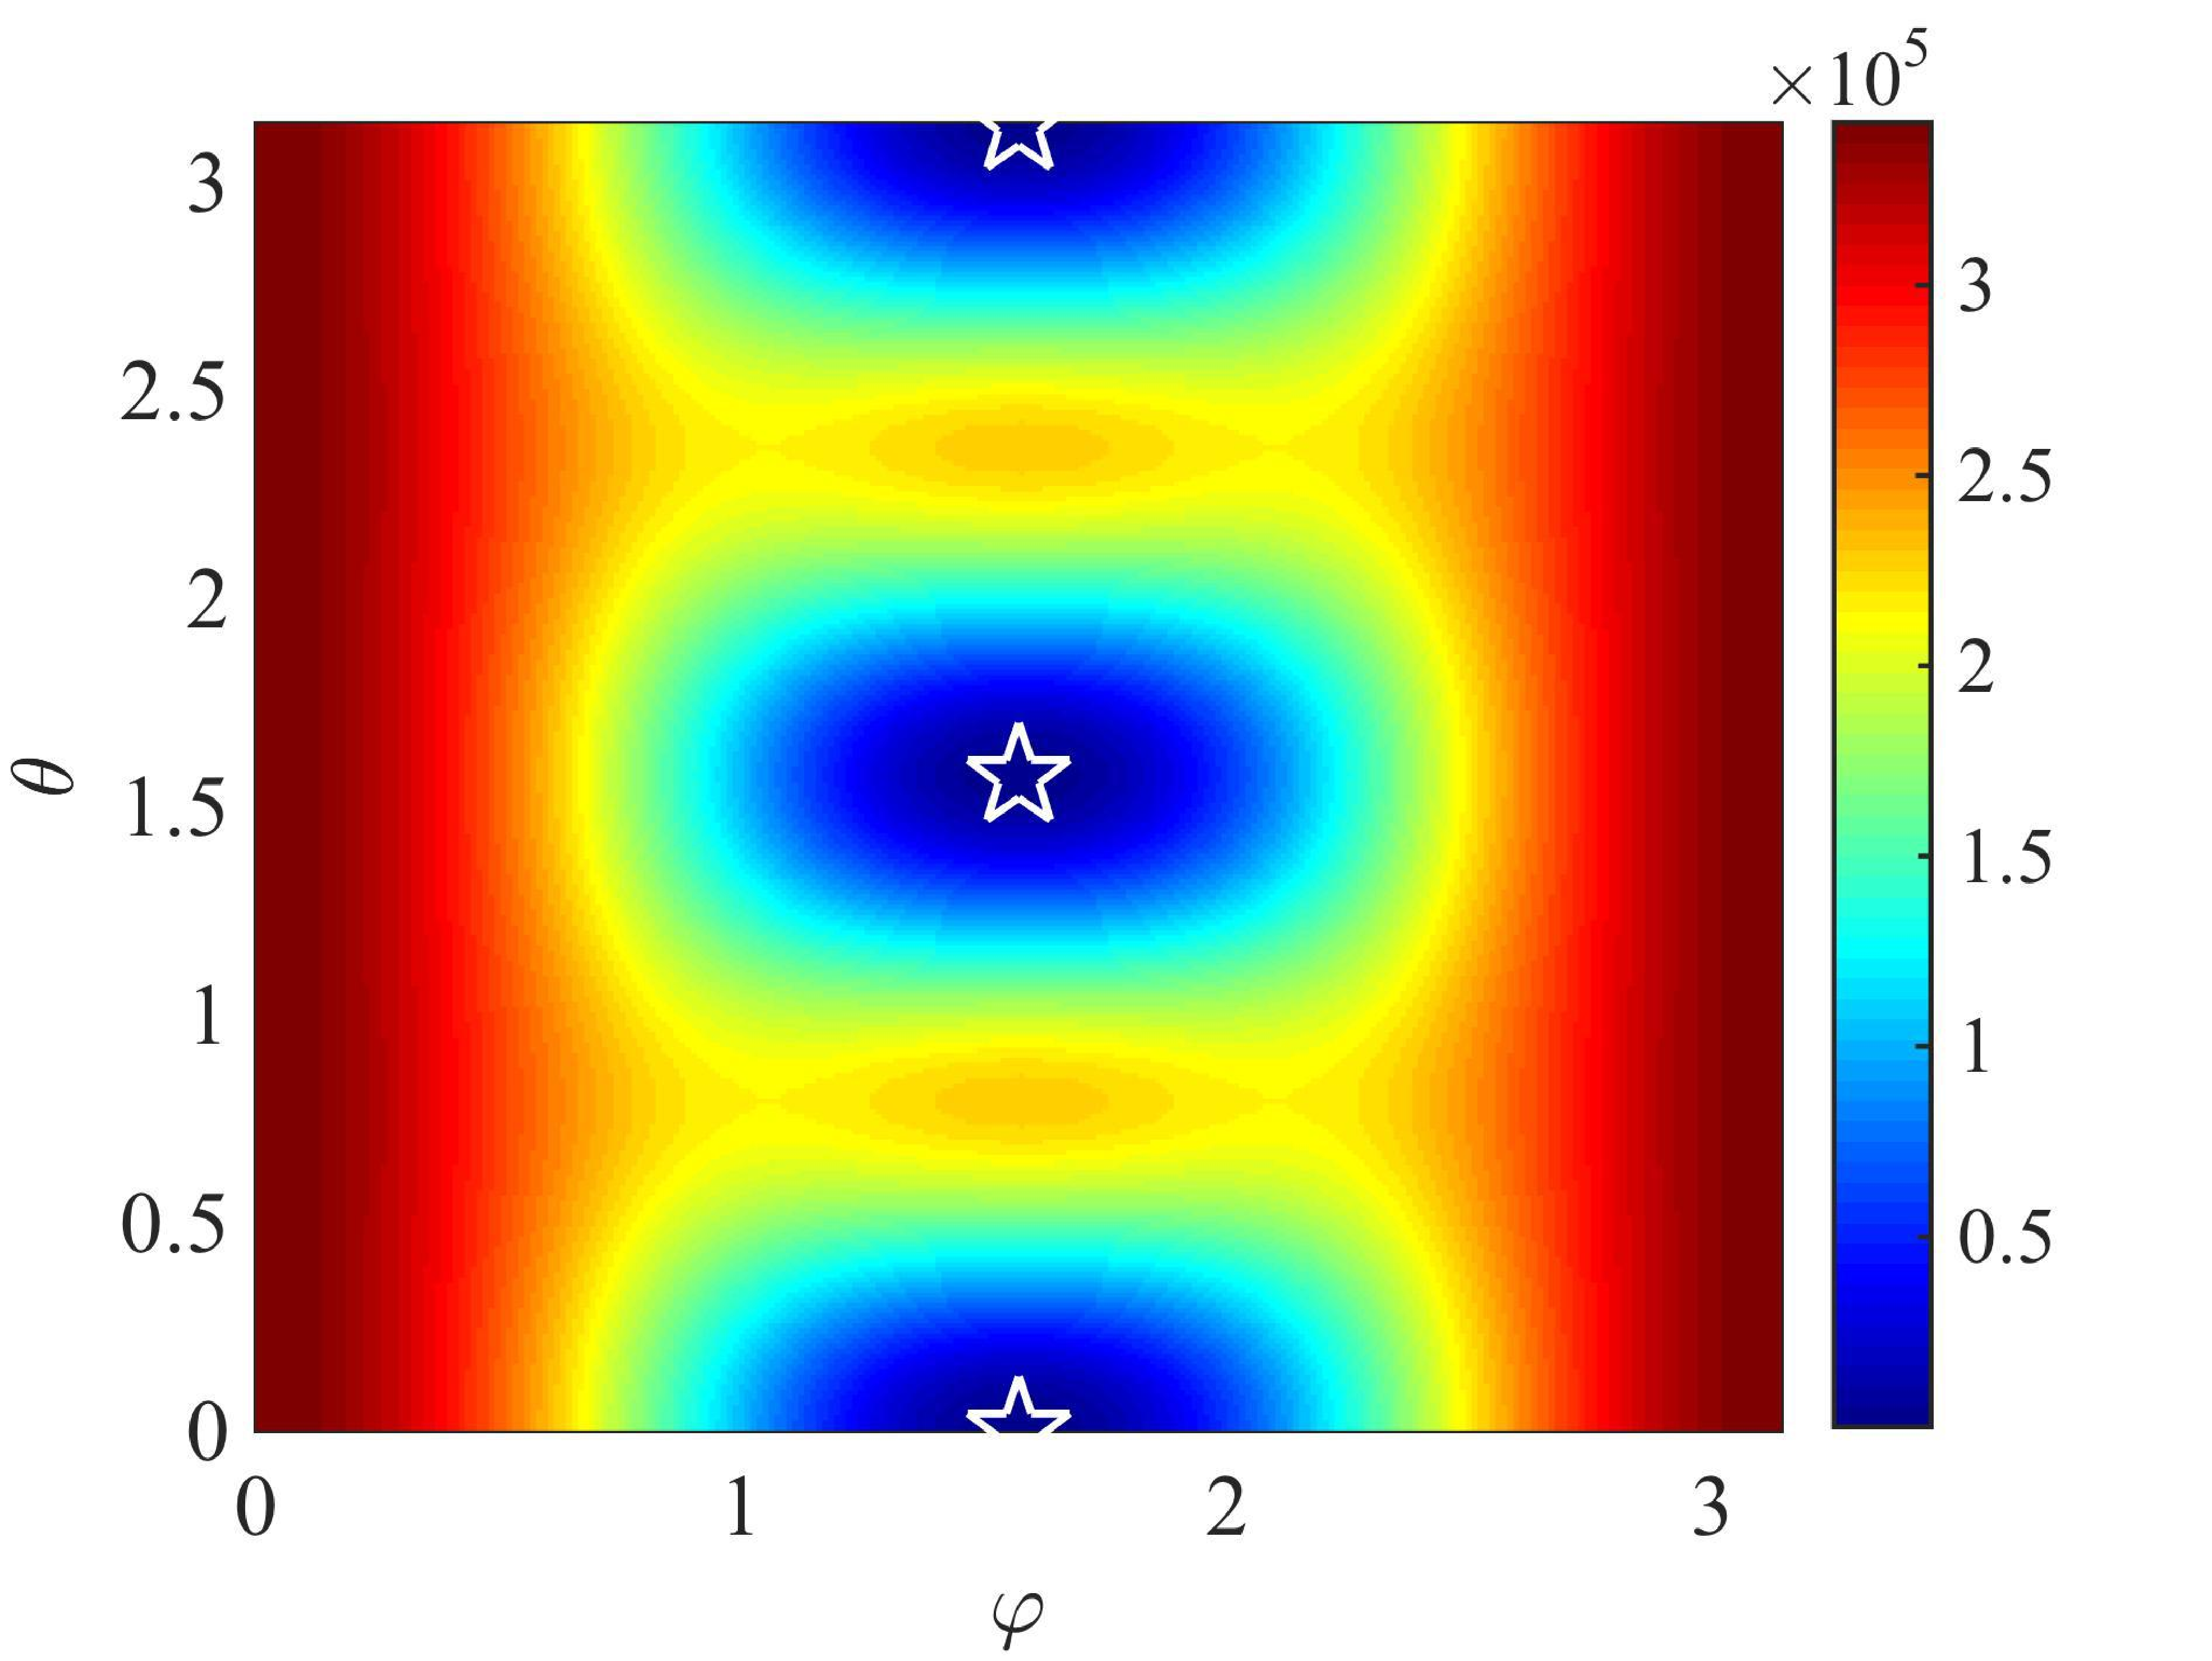
\includegraphics[width=0.45\textwidth]
   {figs/iso_shear_spherical_detAXplane.pdf}
 } \subfigure[Cartesian]{
   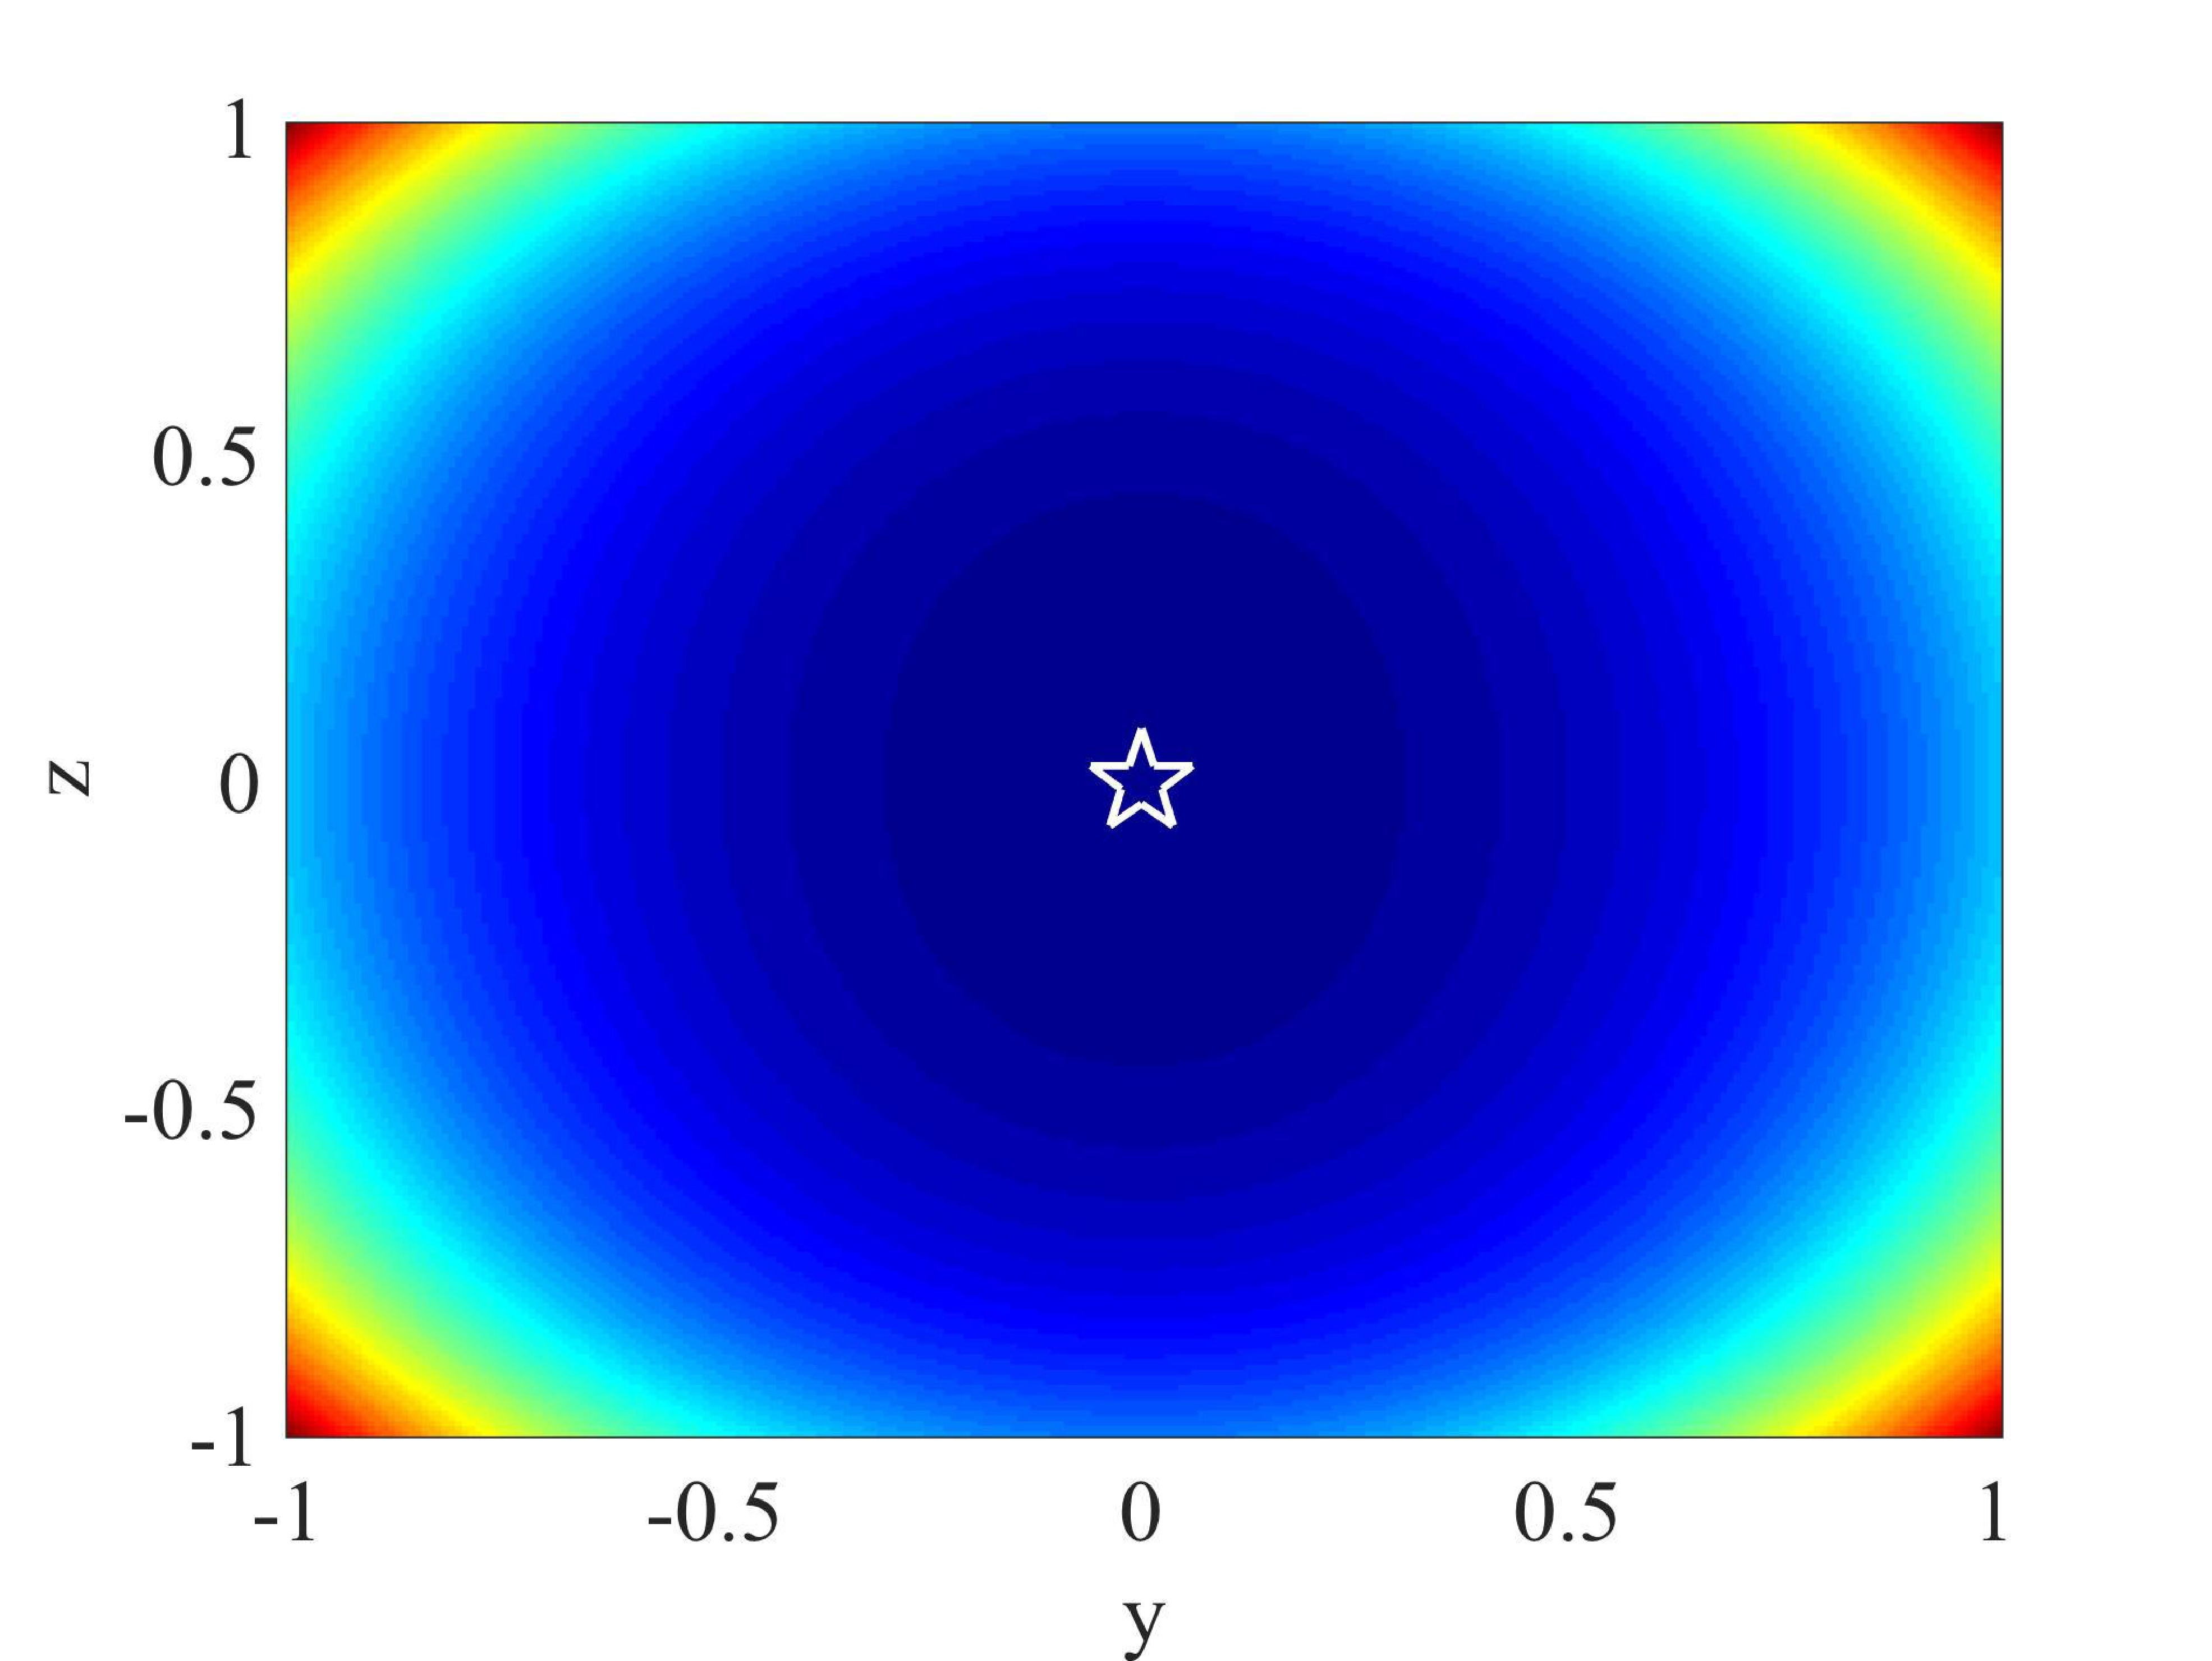
\includegraphics[width=0.45\textwidth]
   {figs/iso_shear_cartesian_detAXplane.pdf}
 } \subfigure[Stereographic]{
   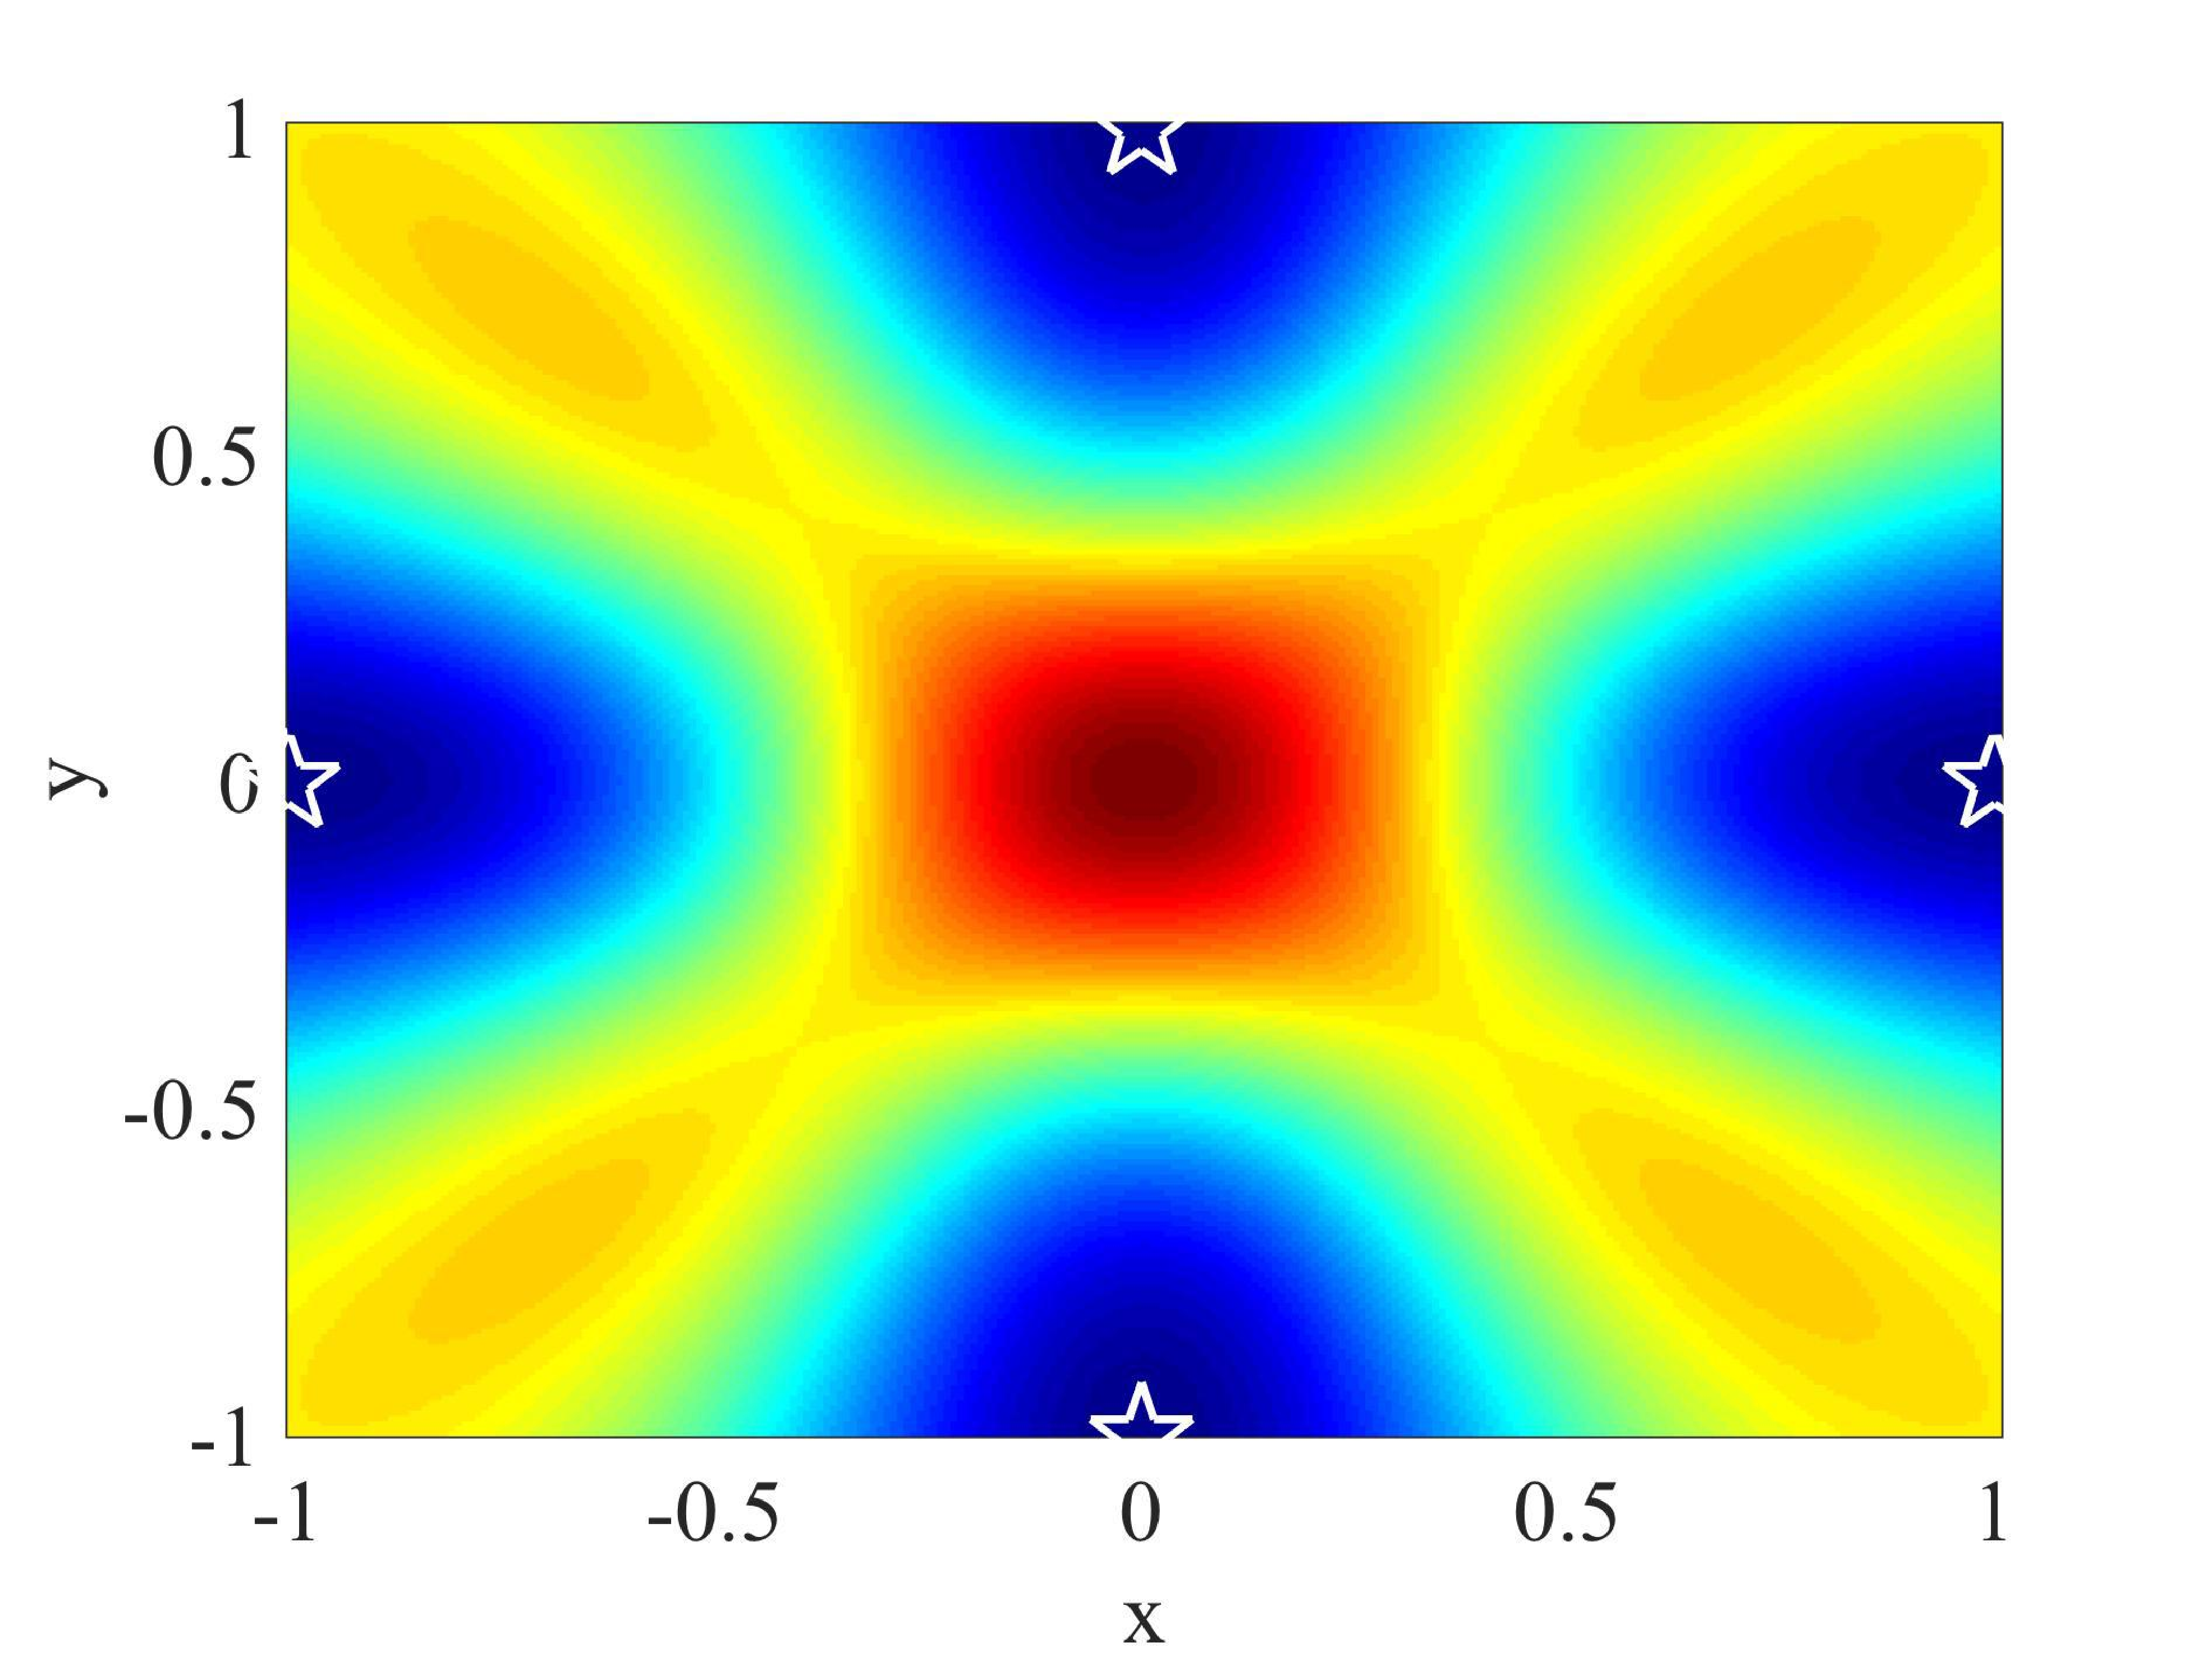
\includegraphics[width=0.45\textwidth]
   {figs/iso_shear_stereographic_detAXplane.pdf}
 } \subfigure[Tangent]{
   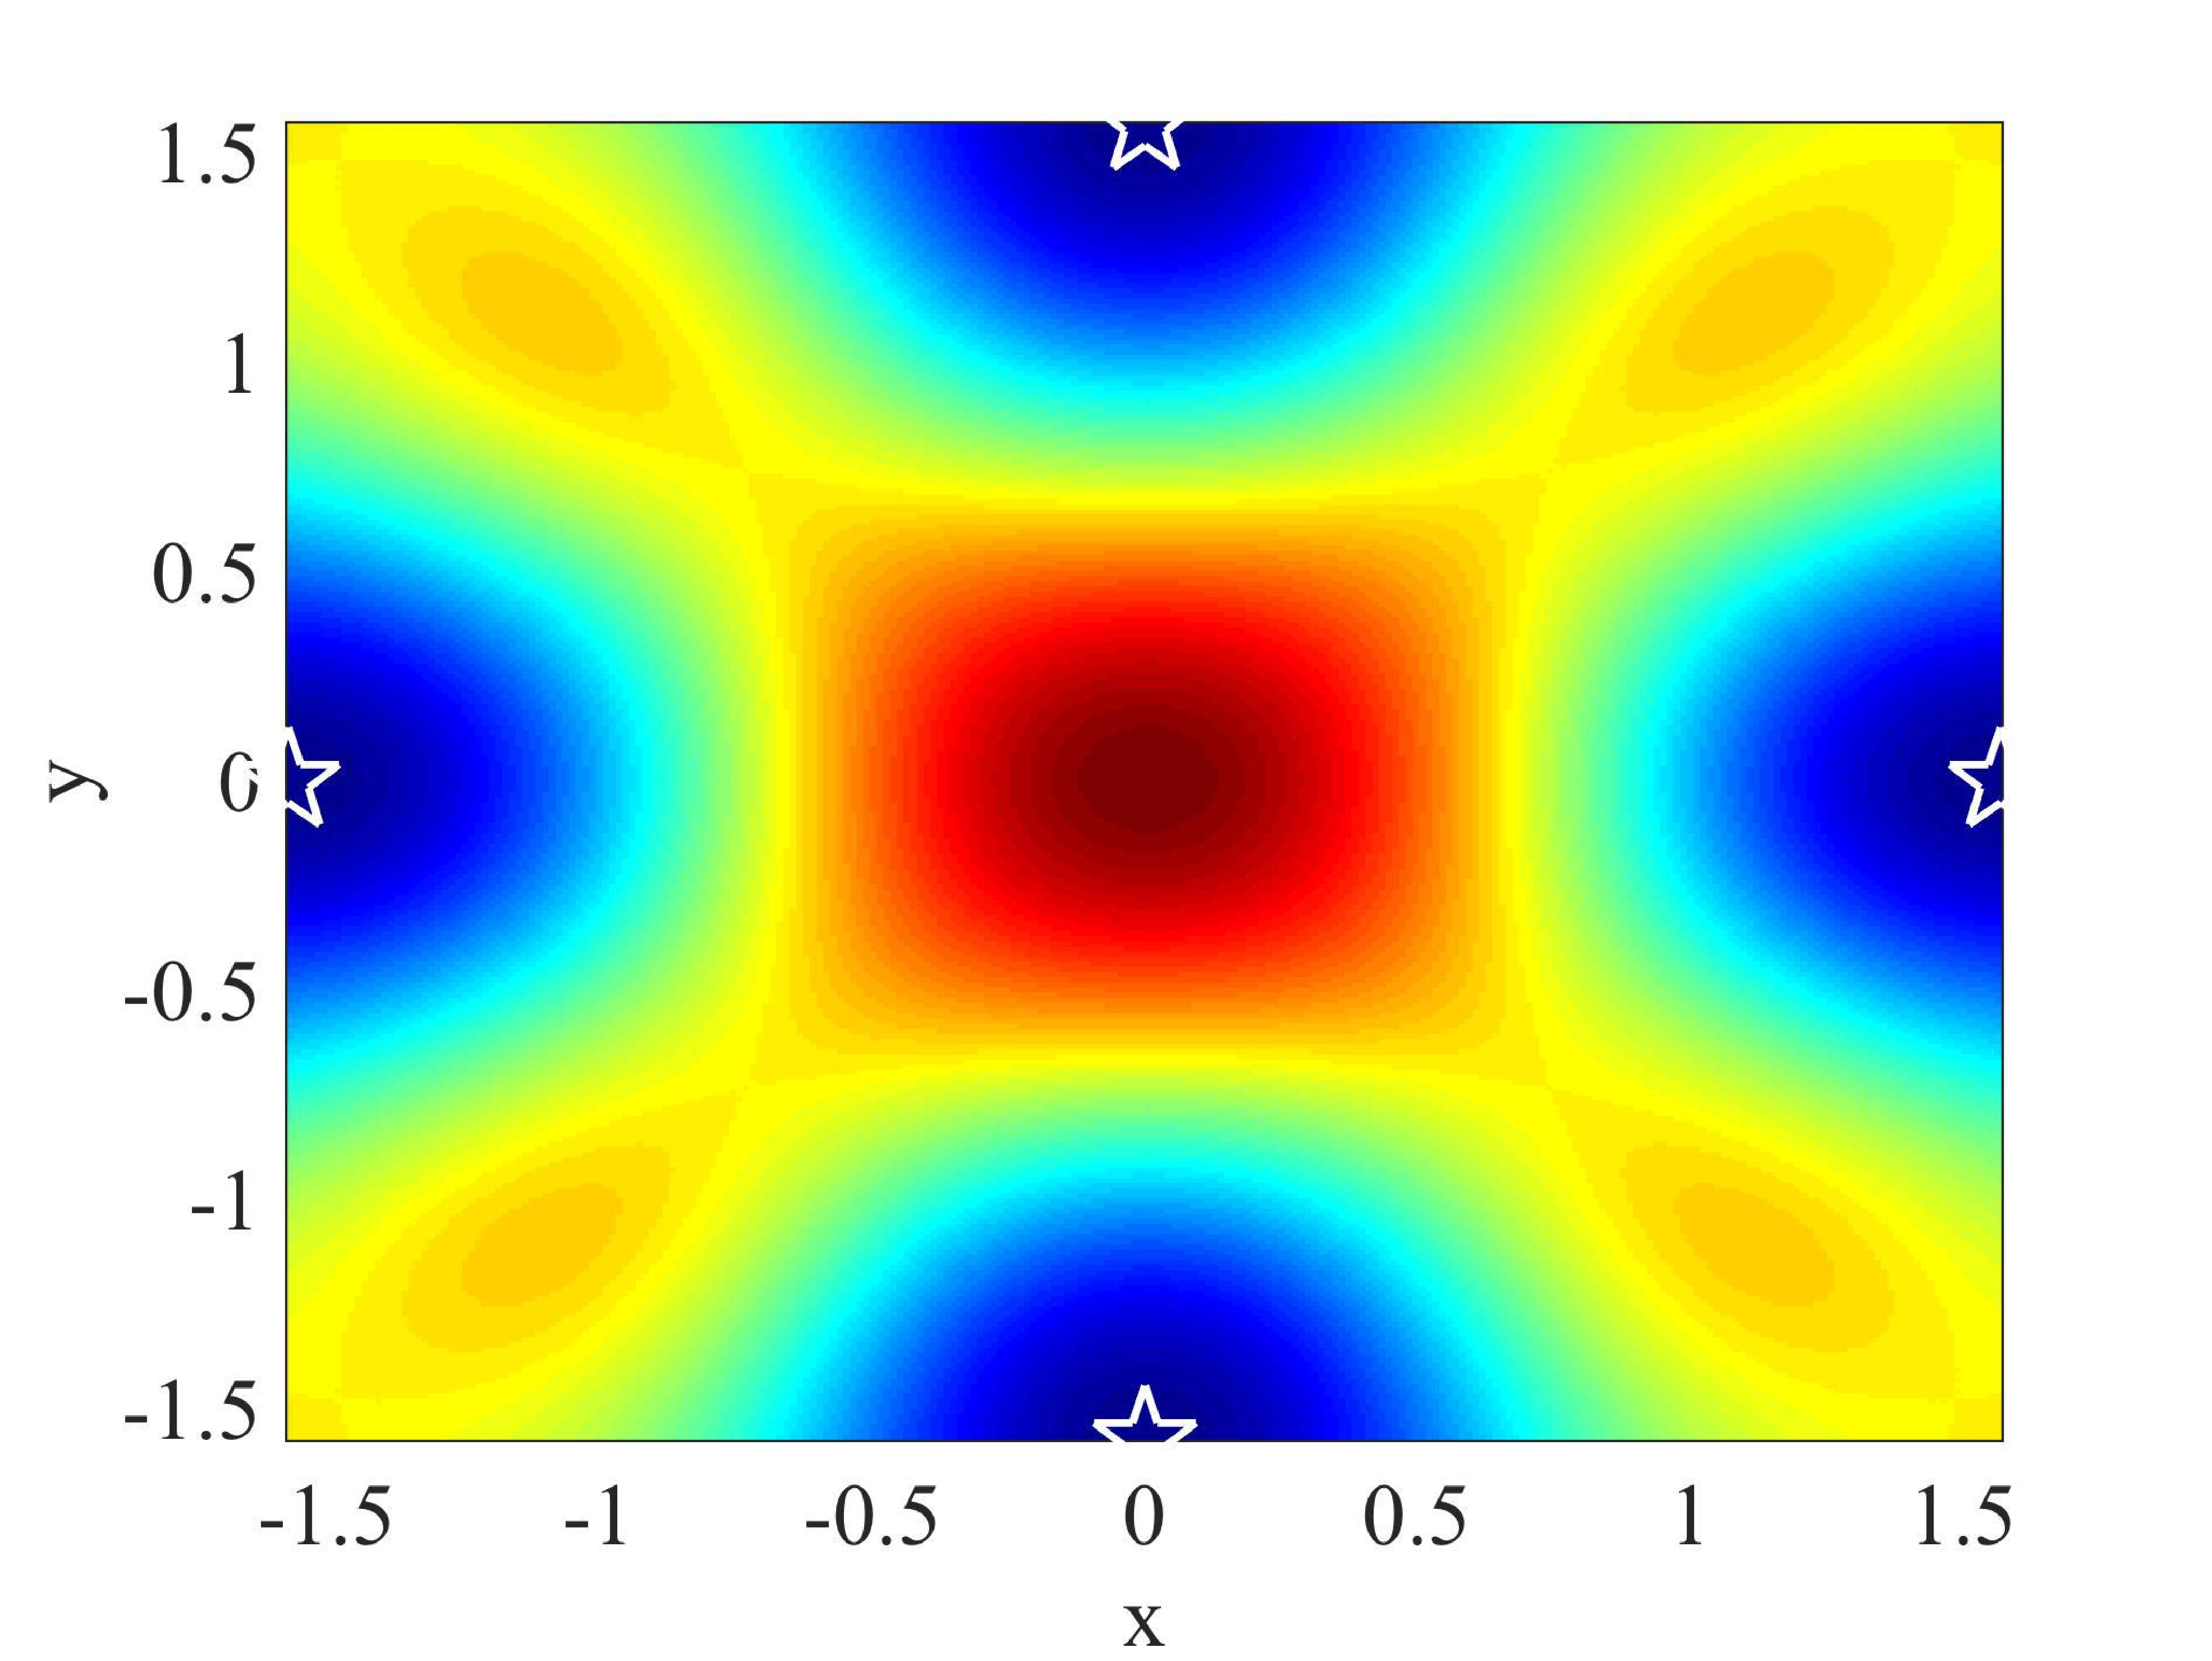
\includegraphics[width=0.45\textwidth]
   {figs/iso_shear_tangent_detAXplane.pdf}
 }
   \caption{Plane views det$\bA$ landscapes at bifurcation
   for simple shear test on small deformation isotropic damage model. 
   The white stars indicate global minimum point in the landscape.}
   \label{fig:iso_shear_detAXplane}
 \end{figure}

From the landscape plots, it is clear that the complexity of the 
determinant function depends greatly on the choices of 
parametrization. Even for a very simple small deformation isotropic 
model adopted in this example, the landscape of the determinant 
function can be quite complex as in the cases of spherical, 
stereographic and tangent parametrizations. 

The Cartesian parametrization results in a simple `bowl-shaped' 
objective function, which makes the Newton-type iterative solve 
particularly robust and insensitive to the initial guess. This has 
been shown in Table~\ref{tab:iso_shear_runtime} and will be 
elaborated further when the initial sweep is eliminated. 

To further analyze the robustness of different parametrizations, we 
compare their performance when there is no sweep algorithm. To provide 
an initial guess for the Newton iterative solve without a sweep 
algorithm, an initial point is randomly generated within the 
parametric space for each parametrization. The tangent modulus at the 
bifurcation step, i.e., when $\epsilon_{12}=0.0559$, is used. If the 
parametrization is able to correctly detect the onset of bifurcation 
and its associated directions, the parametrization is said to succeed 
for this one set of randomly generated parameters. This process is 
repeated for 1000 times, i.e., 1000 sets of random initial guess for 
each parametrization are generated.

Table~\ref{tab:iso_shear_random_para} shows the percentage of 
successful bifurcation detection computed from 1000 runs for all five 
parametrizations. The averaged number of iteration and the 
computational cost of those successful runs are also recorded and 
shown in the table. It can be seen that the proposed Cartesian 
parametrization is much more robust than commonly used spherical 
parametrization, i.e., $100\%$ vs. $42.5\%$ success rate. Cartesian 
also outperforms other uncommon parametrizations. In term of 
computational cost, the Cartesian is also efficient with an averaged 
run time of $170\mu s$.

\begin{table}[H]
  \begin{center}
    %\begin{tabular}{ lp{1.5cm} lp{1.5cm} lp{1.5cm} lp{1.5cm} lp{1.5cm} lp{1.5cm}}
    %  \begin{tabular*}{1.0\textwidth}{l | c c c c c}
    \begin{tabular}{l | c c c c c}
      \toprule
       &  Spherical    &   Stereographic   & Projective   &   Tangent   &   Cartesian                 \\
      \midrule
      Success rate ($\%$)                      &    42.7    &    22.7    &    59.9     &    20.6     &   100          \\ 
      Averaged iteration count               &    12.2    &    4.70    &    8.86     &    5.12     &   5.35          \\
      Averaged run time (${\mu}s$)     &    549     &    242     &    495      &    264      &   207         \\
      \bottomrule
    \end{tabular}
    \caption{Isotropic small deformation model: success rate and computational cost of Newton iterative solve with a single random initial point. A total of 1000 random trials are performed for each parametrization.}
    \label{tab:iso_shear_random_para}
  \end{center}
\end{table}

As aforementioned, the superior performance of the proposed Cartesian 
in term of computational efficiency and robustness can be attributed 
to its relatively simple determinate function landscape, which makes 
the Newton iterative solve easier to converge. Figure~
\ref{fig:iso_shear_robust} shows the contour of the determinant 
function used in the above robustness  study. 1000 random initial 
points are also plotted. If the initial guess leads to a success 
detection of bifurcation and its directions, the point will be marked 
as a solid circle ($\bullet$). Otherwise, it will be marked as a cross 
($\times$). This figure provides a very direct visualization of the 
robustness study results. 

\begin{figure}[H]
   \centering \subfigure[Spherical]{
   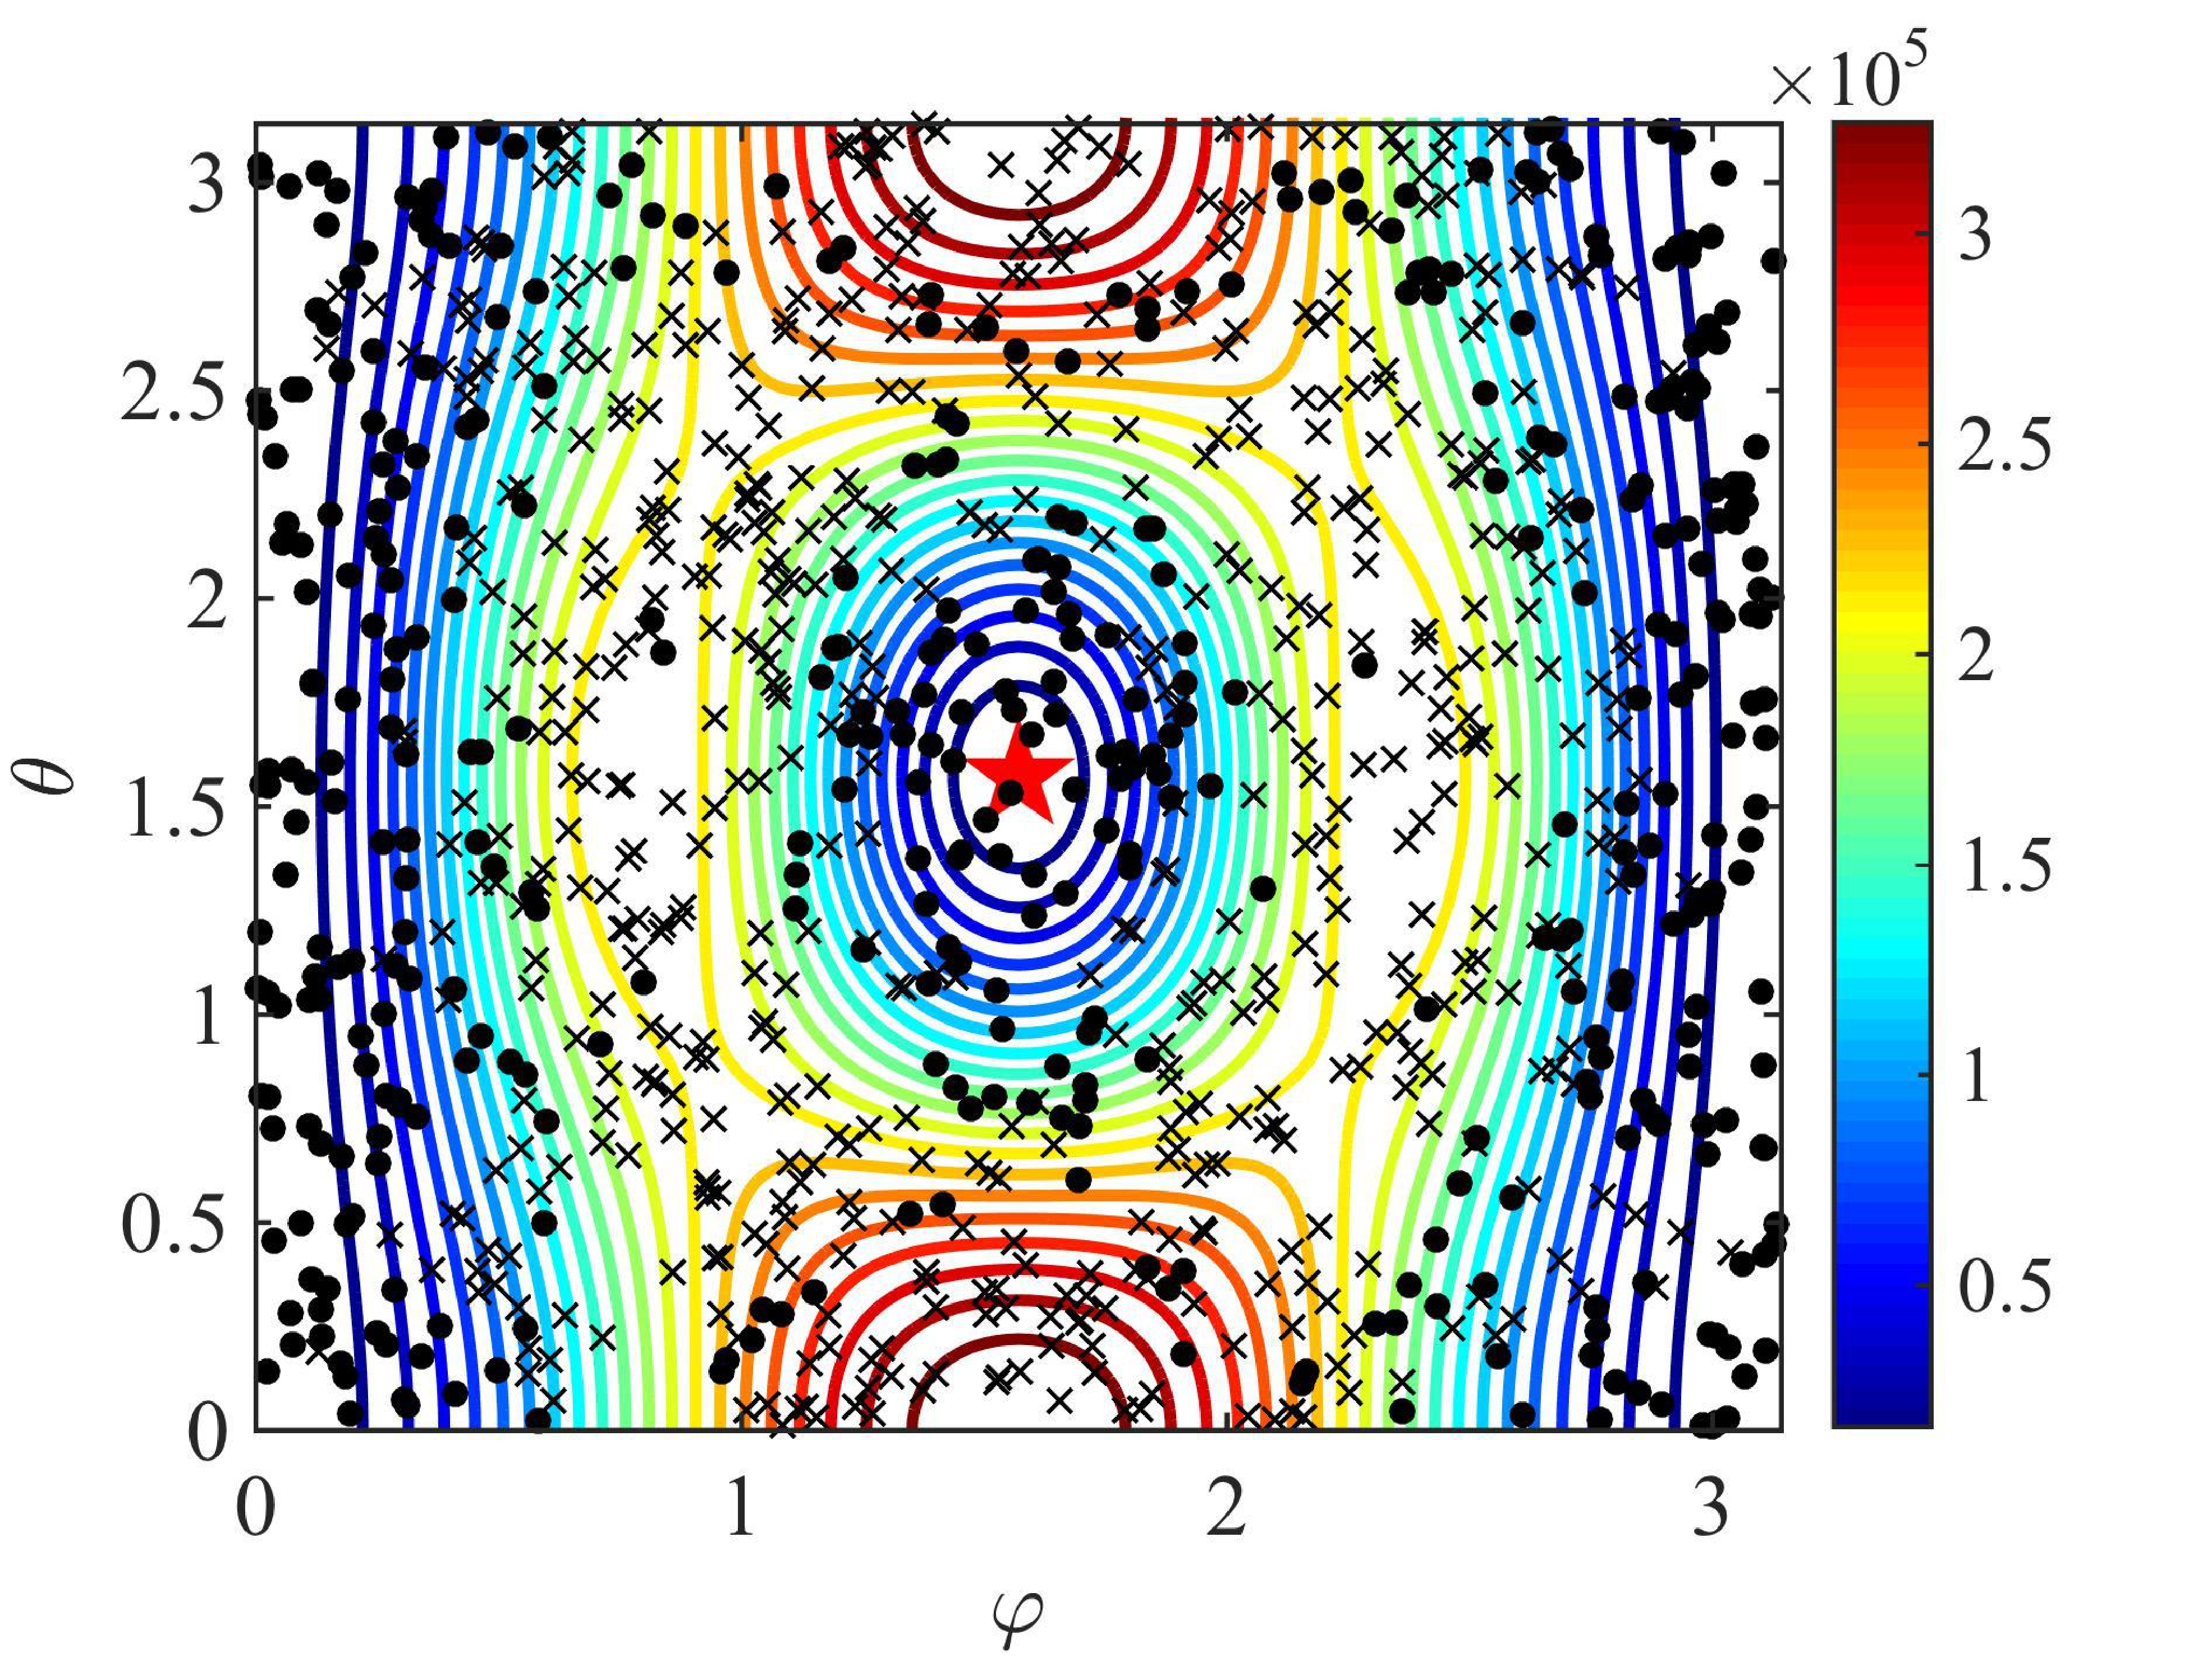
\includegraphics[width=0.45\textwidth]
   {figs/iso_shear_spherical_random.pdf}
 } \subfigure[Cartesian]{
   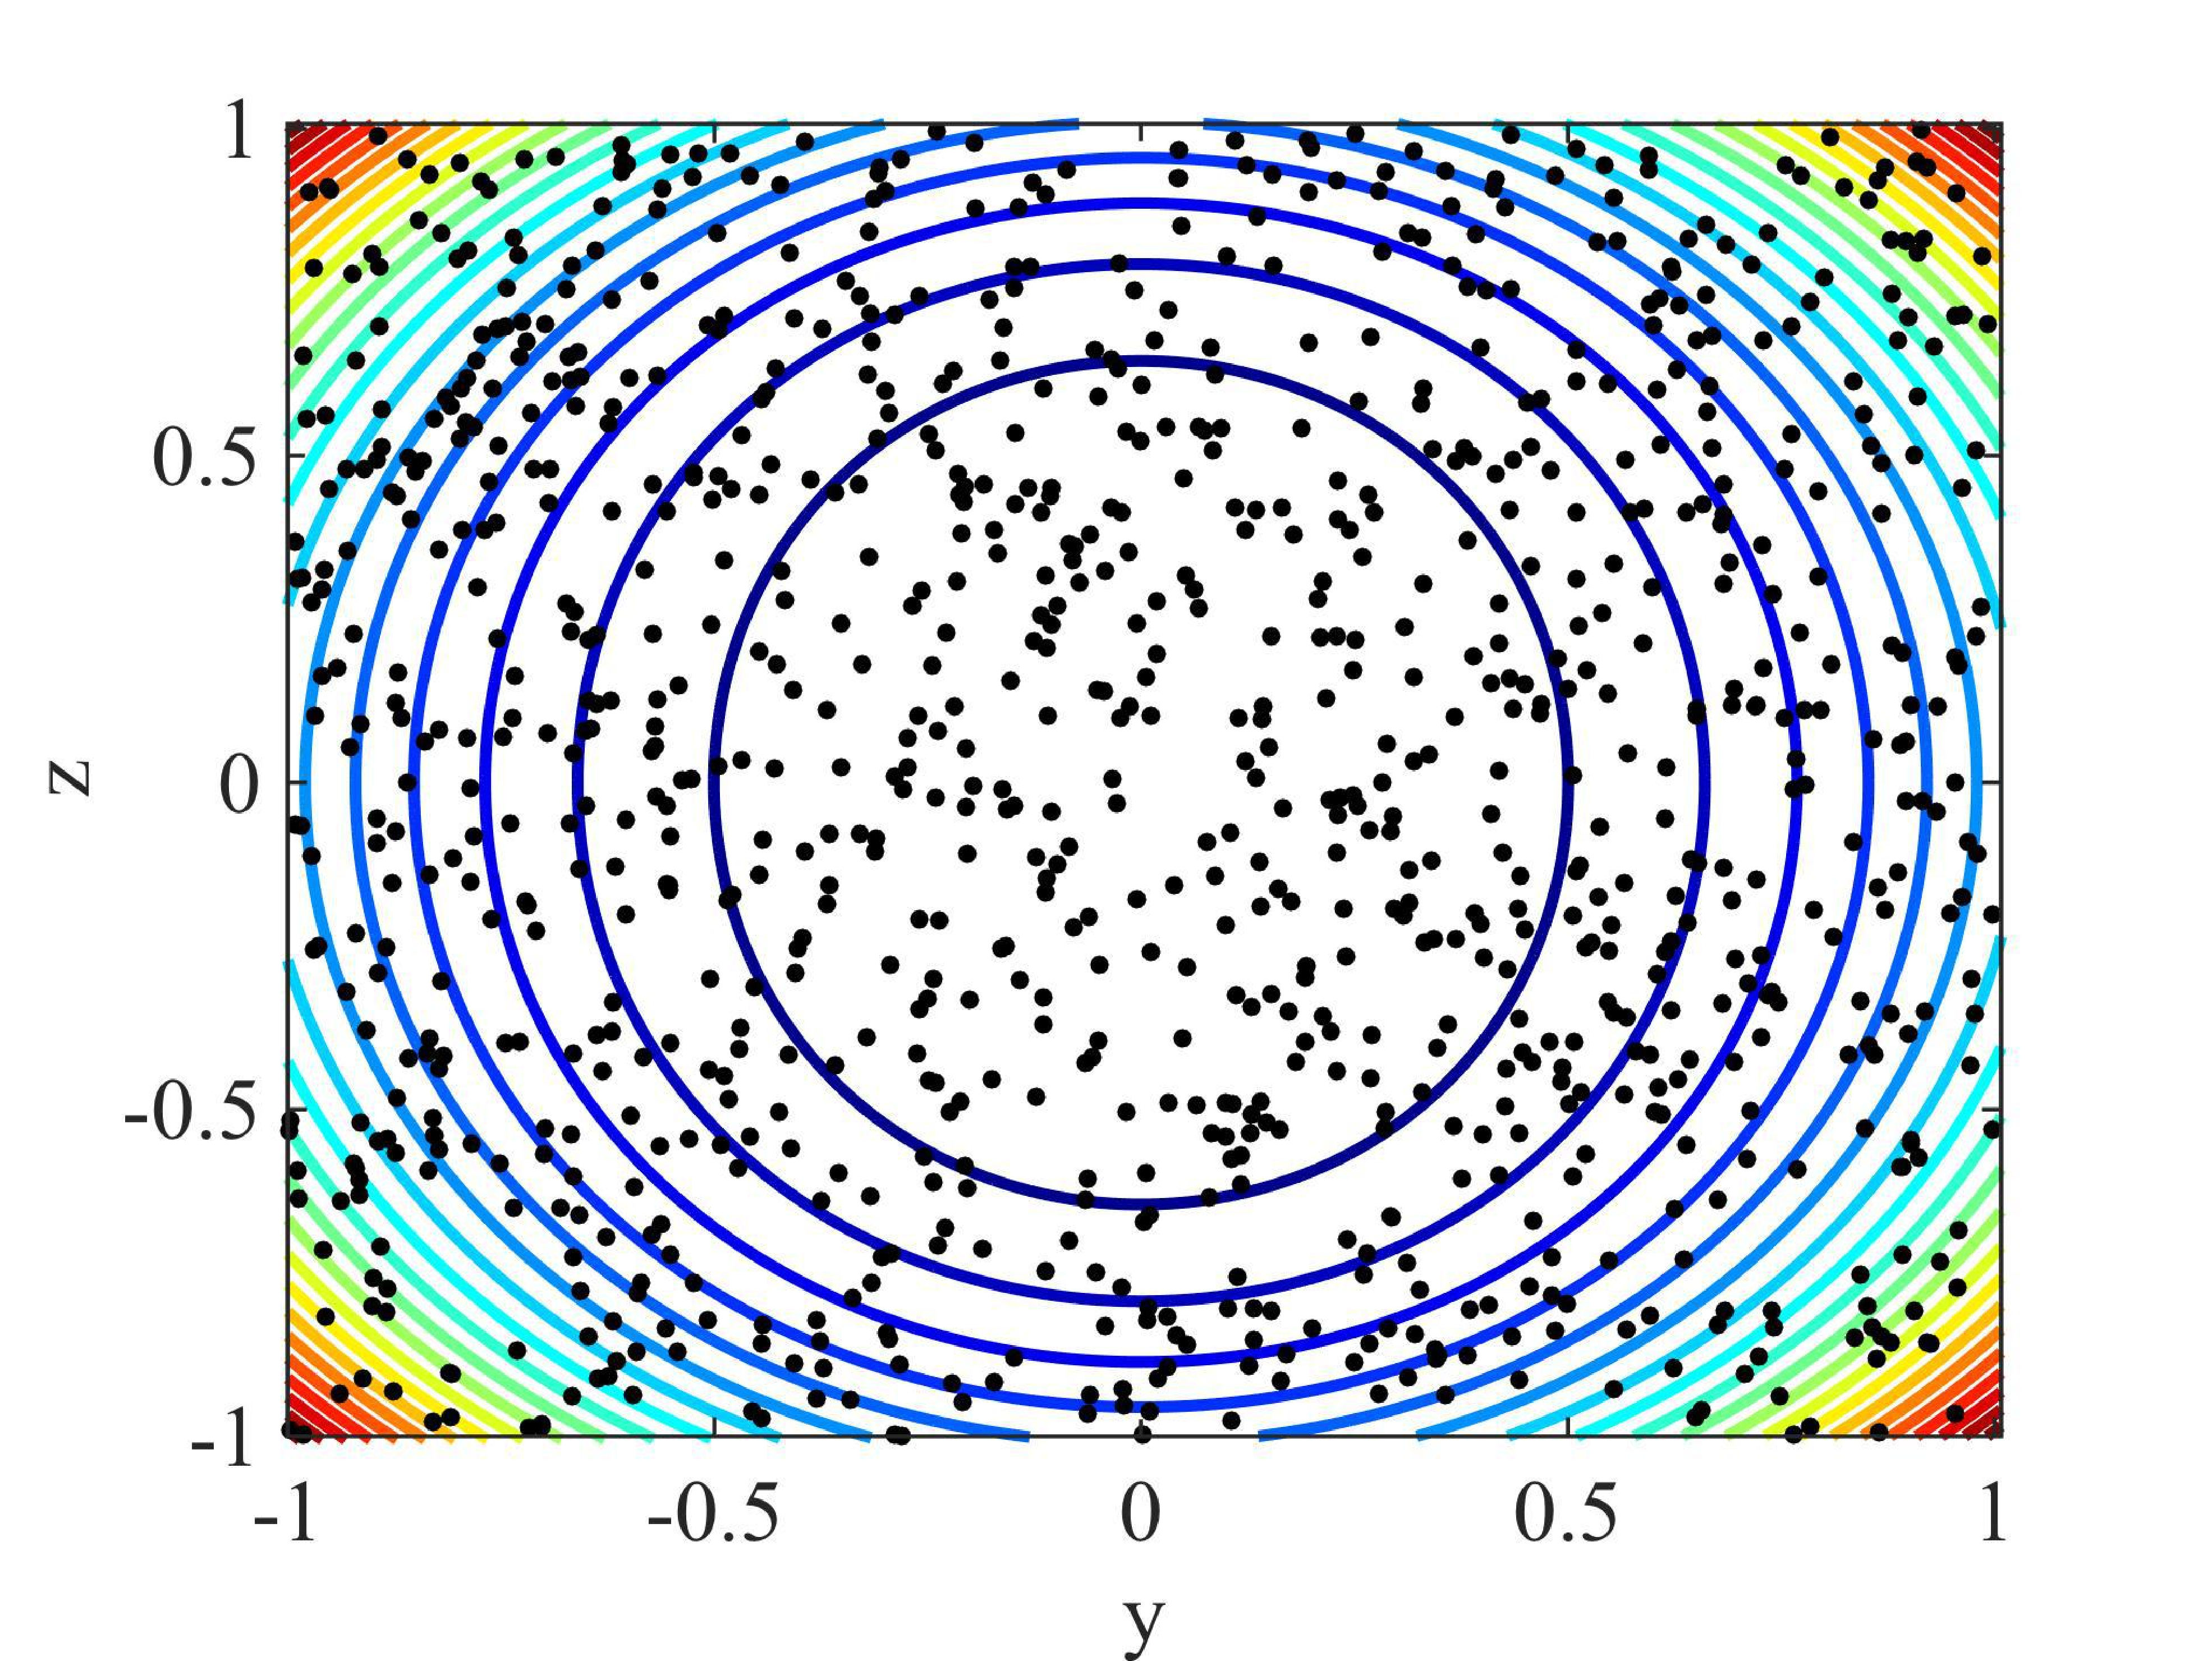
\includegraphics[width=0.45\textwidth]
   {figs/iso_shear_cartesian_random.pdf}
 } \subfigure[Stereographic]{
   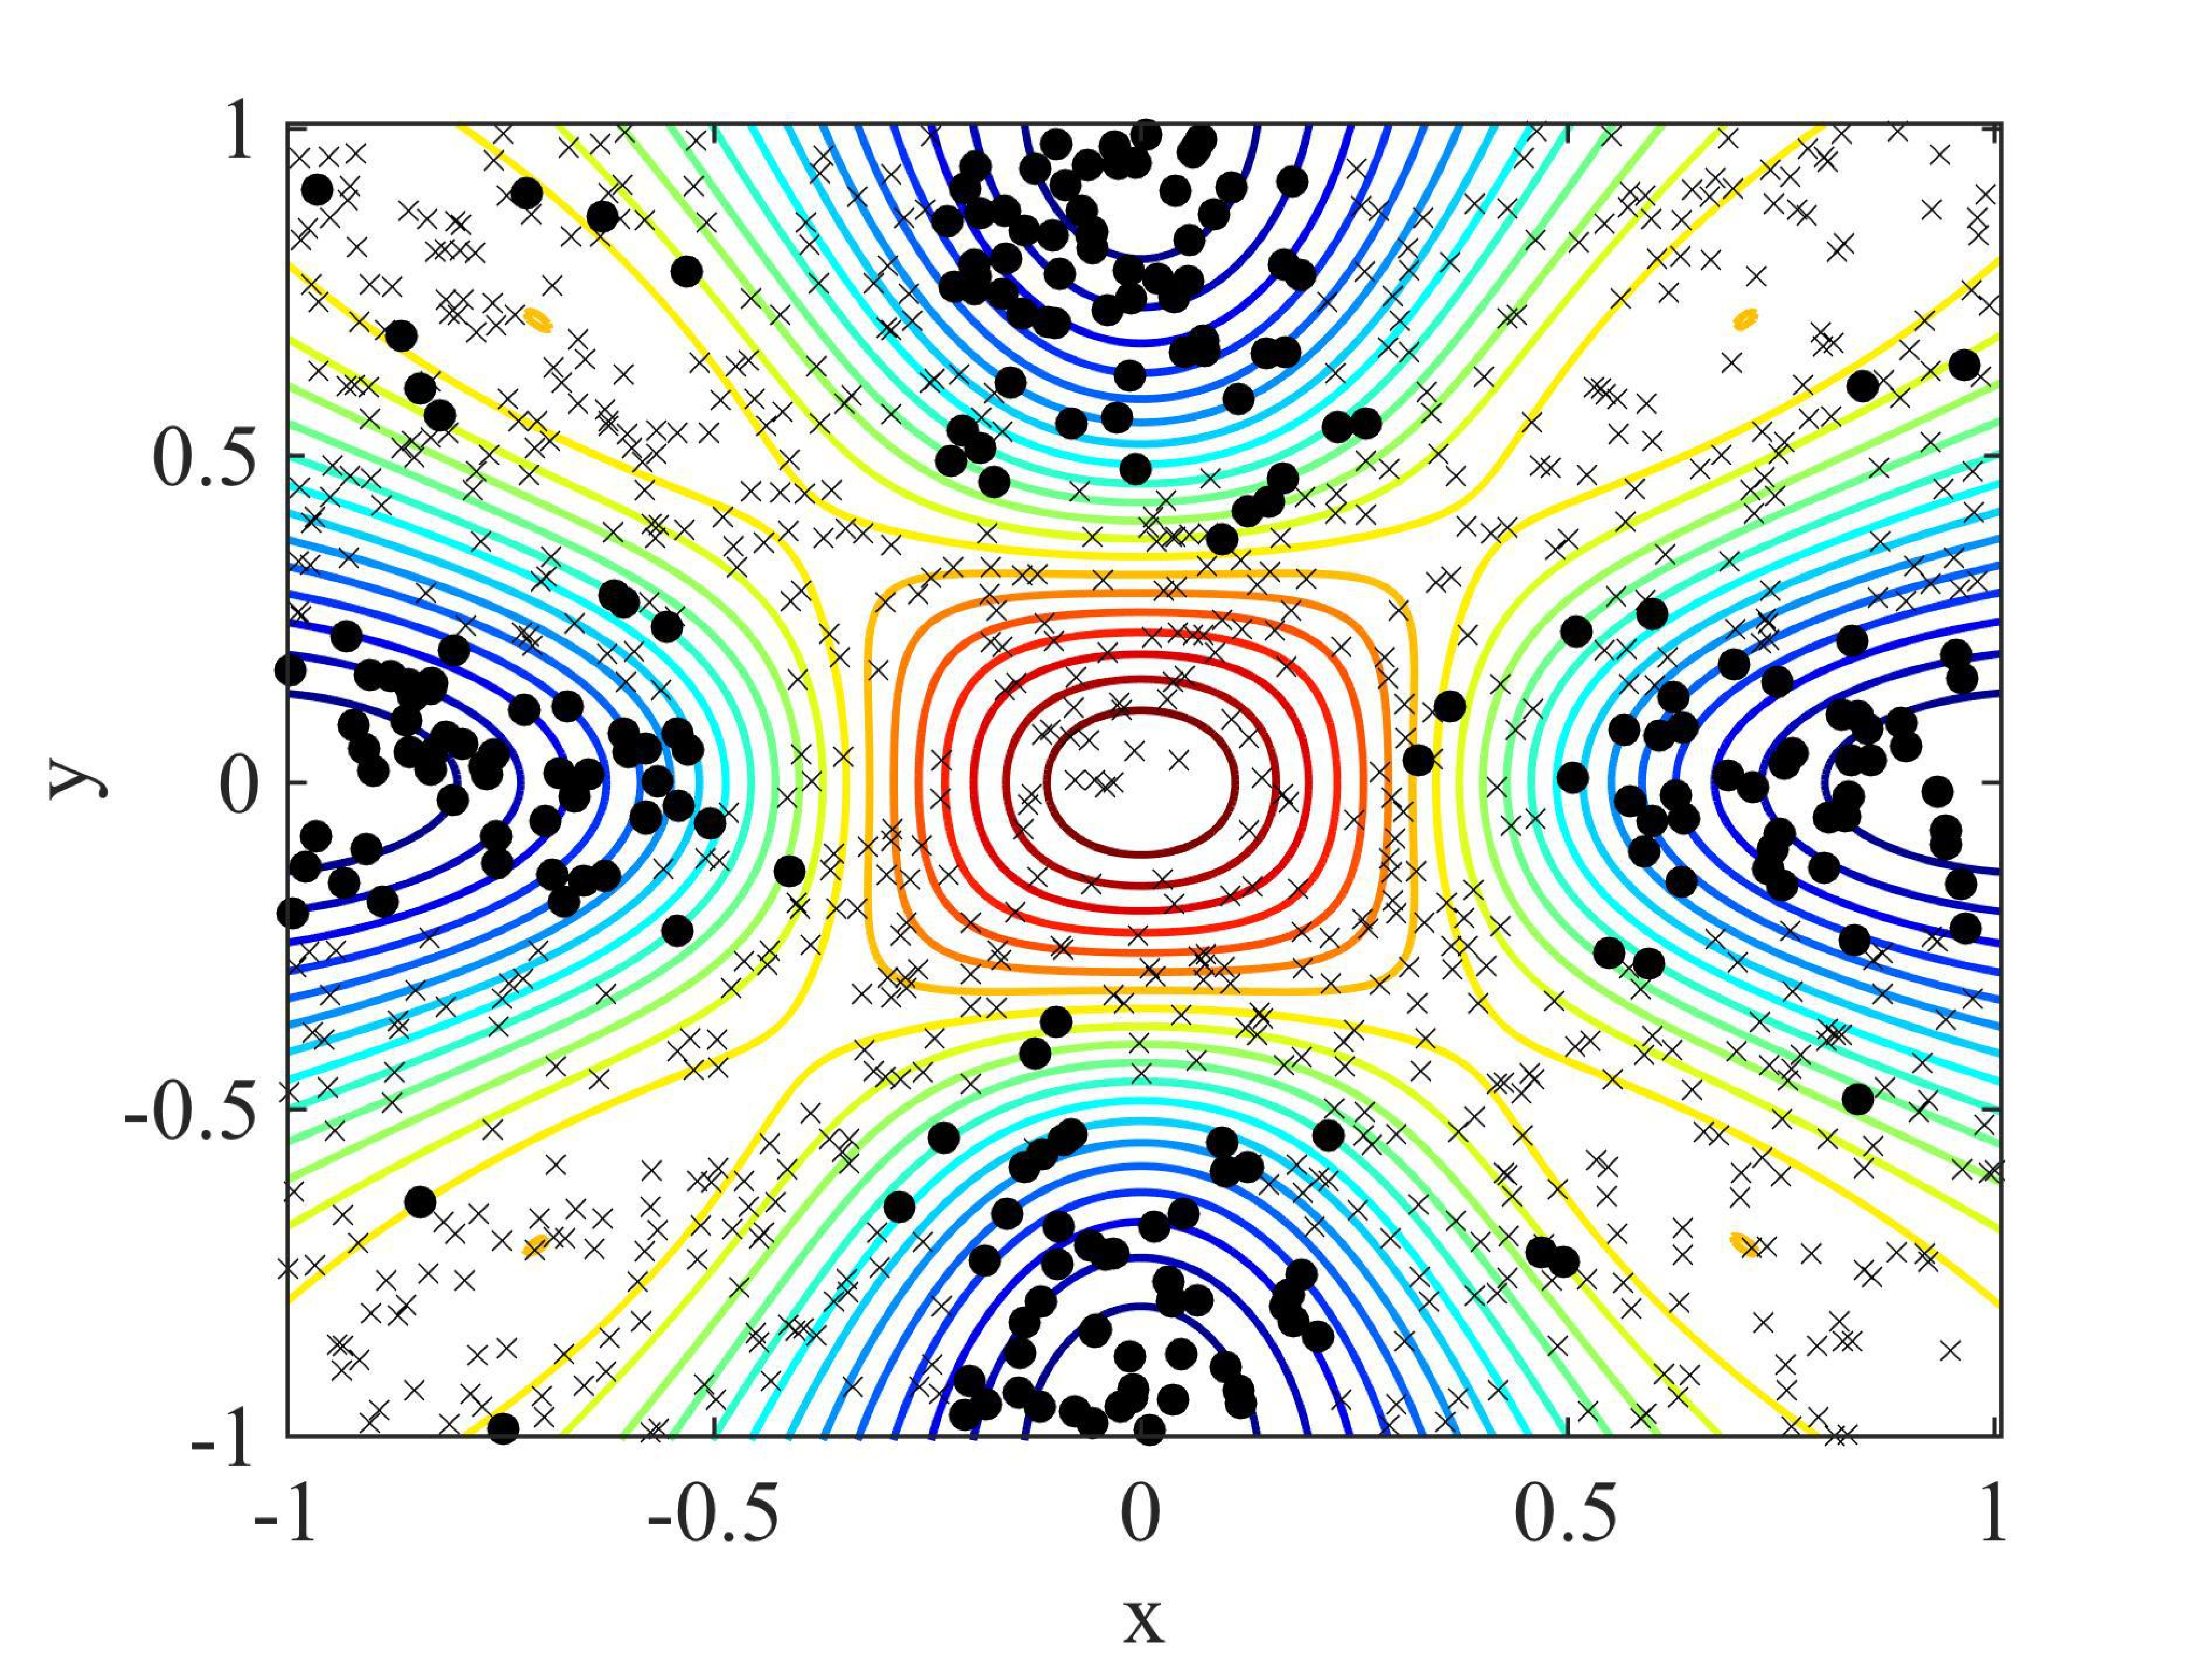
\includegraphics[width=0.45\textwidth]
   {figs/iso_shear_stereographic_random.pdf}
 } \subfigure[Tangent]{
   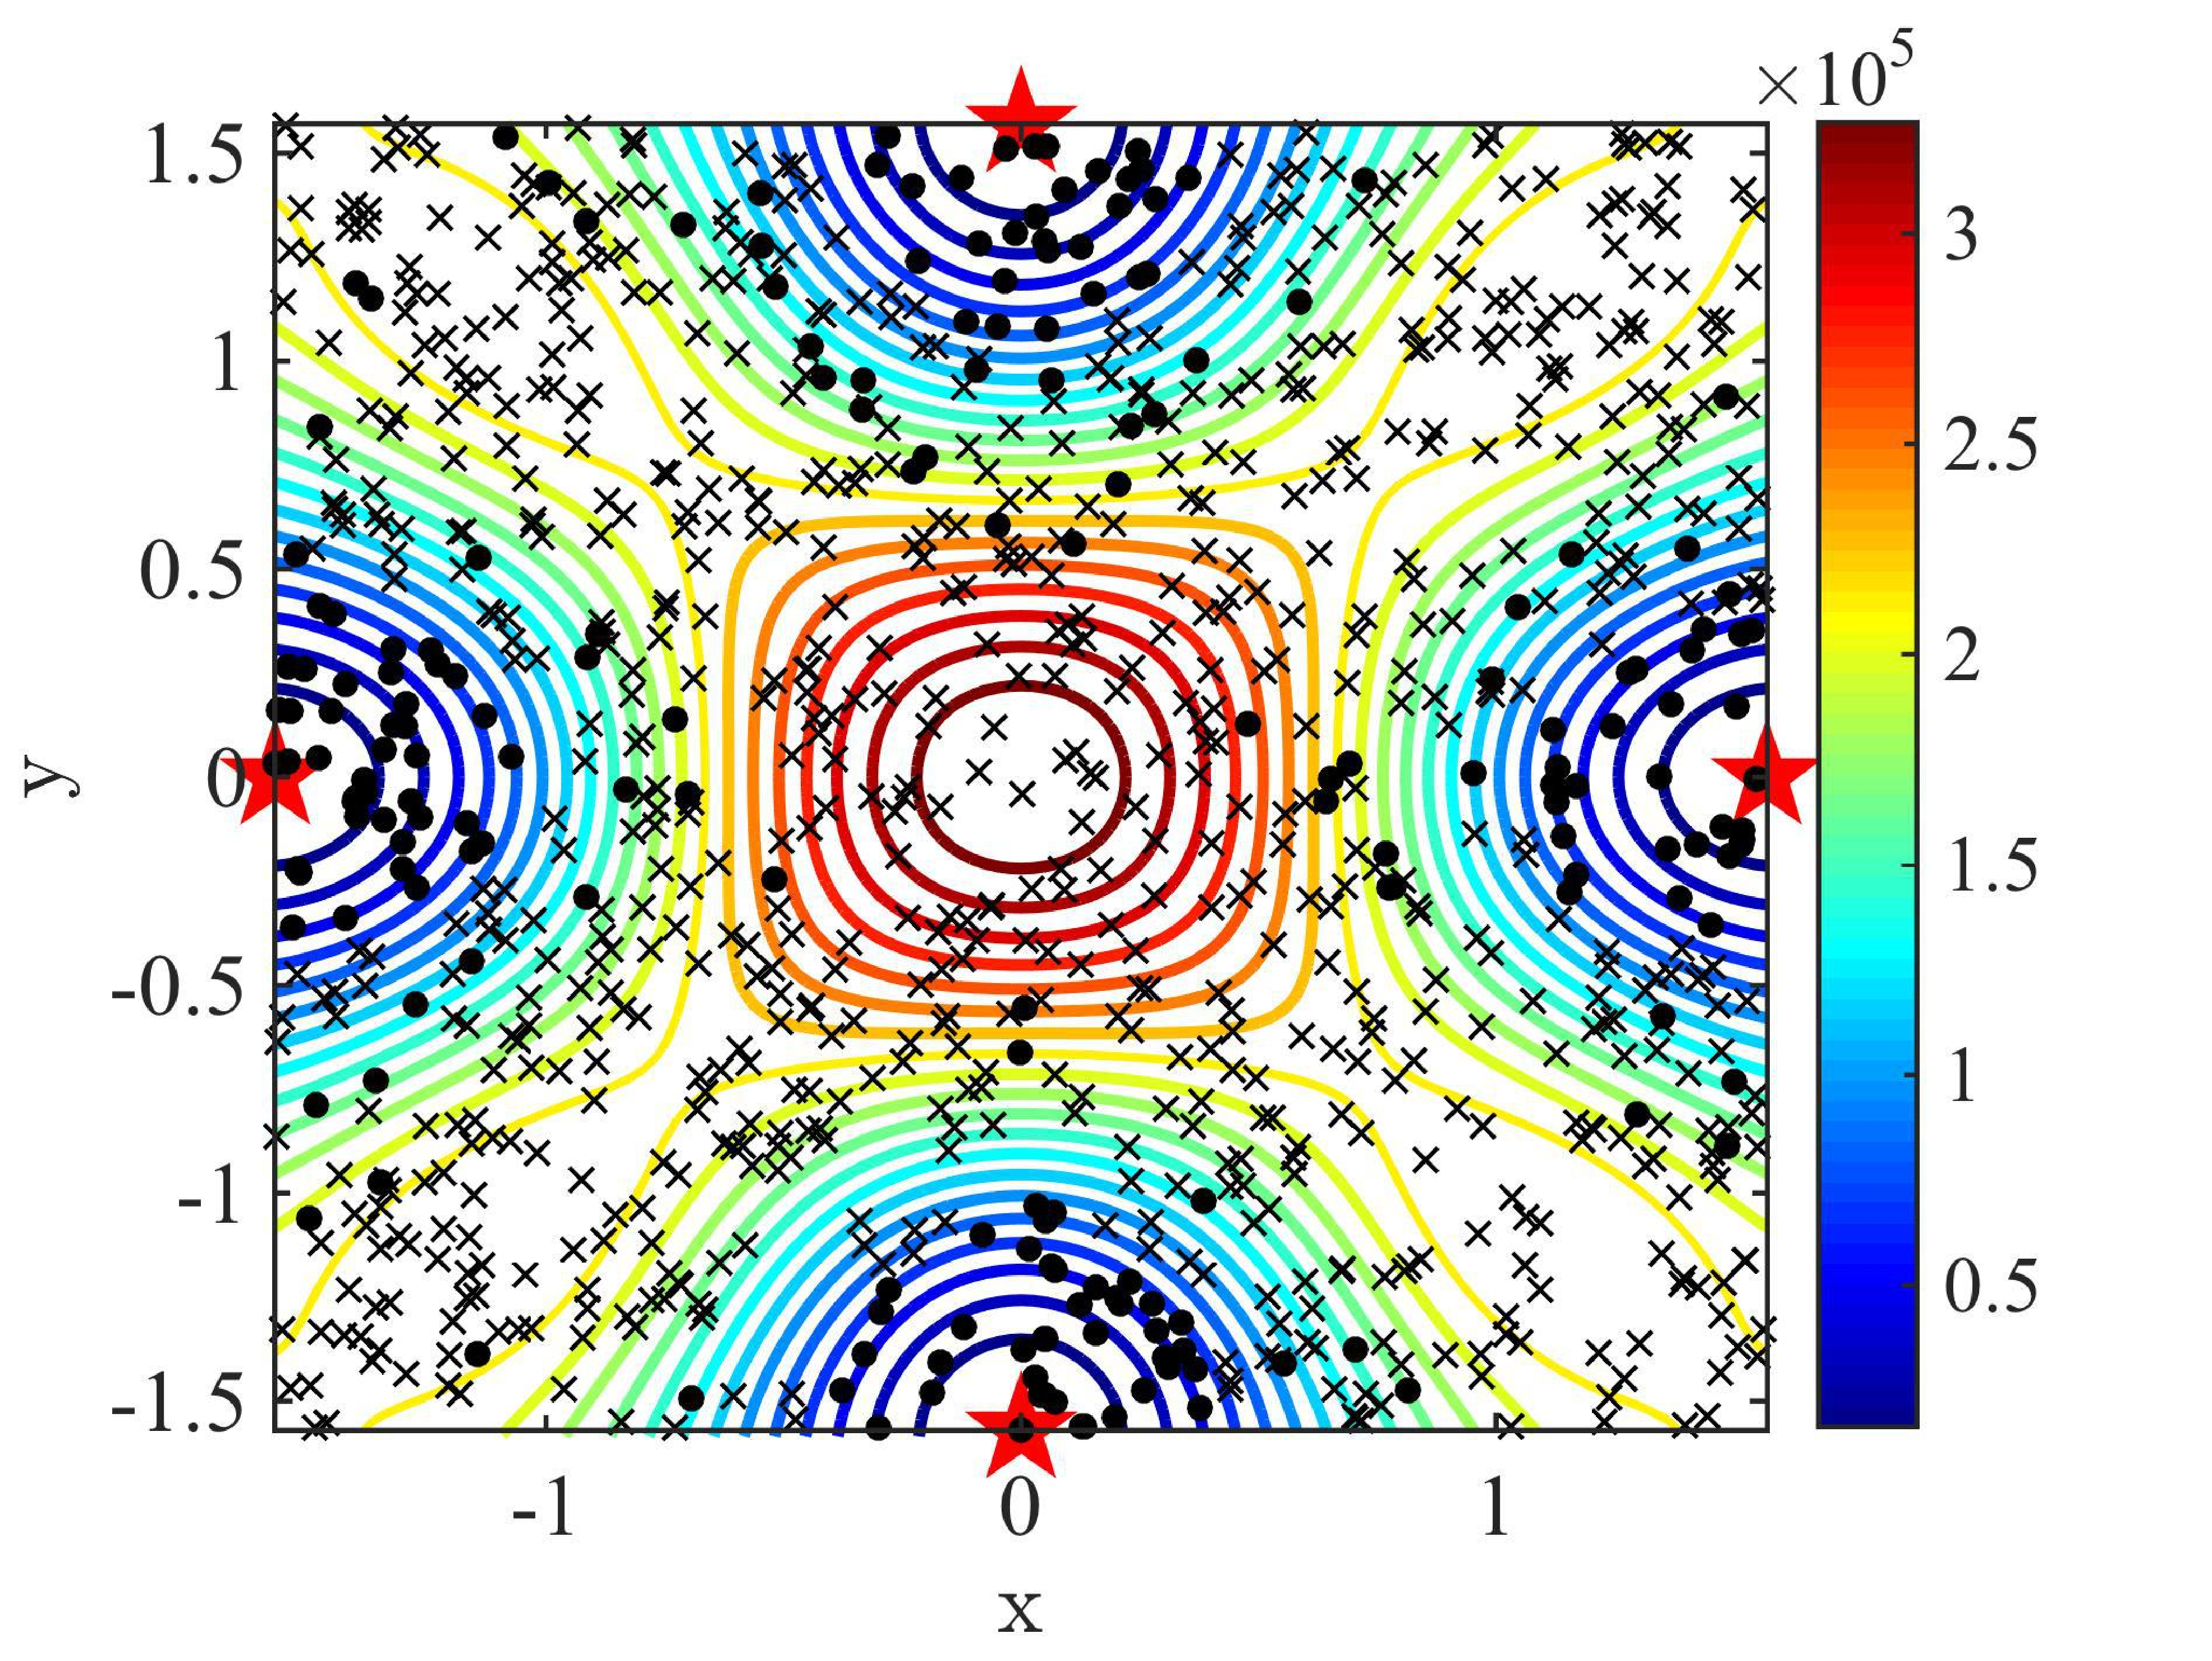
\includegraphics[width=0.45\textwidth]
   {figs/iso_shear_tangent_random.pdf}
 }
   \caption{Isotropic small deformation model: results of Newton 
   iterative solve with a single random initial point plotted on the 
   contour of determinant function at bifurcation. A solid circle 
   ($\bullet$) means the initial point leads to a success detection of 
   bifurcation and its directions. A cross ($\times$) means the Newton 
   iterative solve fails. A total of 1000 random trials are performed 
   for each parametrization.}
   \label{fig:iso_shear_robust}
\end{figure}

\subsection{Finite deformation anisotropic hyperelastic damage model}
\label{subsec:anisotropic}

The second material model tested is a finite deformation anisotropic 
hyperelastic damage model. By adding complexity to the material model, 
and hence the tangent modulus, we would like to study how will the 
performance of different parametrizations be affected. As in the 
previous example, we first present the key feature of the material 
model.

\subsubsection{Model formulation}

The free energy function of the finite-deformation anisotropic 
hyperelastic damage model consists of an isotropic term and direction-
dependent terms. This type of energy formulation is motivated to 
capture behavior of materials with an isotropic matrix and some 
microfibers with preferred directions, such as the model proposed by
\citet{Chen.etal:2014} to capture behavior of hydrided nuclear 
cladding materials. We assume that the damage affects both the matrix 
and the microfibers. The free energy function is proposed to have the 
following form:

\begin{equation}\label{eq:aniso_energy}
  \Psi (\bC, \bM, \xi_m, \xi_i) 
    = (1-\xi_m) f_m \Psi_m^0(\bC) 
    + \sum_{i}^{n} (1-\xi_i) f_i \Psi_i^0(\bC, \bM)
\end{equation}

where $\bC$ is the Right Cauchy-Green tensor, $\bM$ is a
unit vector characterizing the preferred fiber direction, $f_m$ and 
$f_i$ are the volume fraction of the matrix and $i$th fiber, $n$ is 
the number of fiber terms, $\xi_m$ and $\xi_i$ are the damage factors 
corresponding to the matrix and the $i$th fibers, respectively. In the 
following examples, we assume that there are two preferred fiber 
directions, i.e., $n=2$.

We adopt a compressible Neo-Hookean type energy function for the 
effective (undamaged) matrix component

\begin{equation}\label{eq:aniso_Psim0}
  \Psi_m^0 (\bC) 
    = \frac{1}{8}\lambda (\ln I_3)^2
    - \frac{1}{2}\mu \ln I_3 
    + \frac{1}{2}\mu( I_1 - 3)
\end{equation}

where $\lambda$ and $\mu$ are Lam\'{e}'s constant and shear modulus,
respectively.  

For microfibers, we adopt one particular form of strain-energy 
function proposed in \cite{Holzapfel.etal:2010}

\begin{equation}
  \Psi_i^0(\bC, \bM) 
    = \frac{k_i}{q_i}
    \{ \exp[q_i(I_4 - 1)^2] \}
\end{equation}

where $k_i$ and $q_i$ are elastic constants for the $i$th fiber. 
The strain invariants $I_1$, $I_3$ and $I_4$ are defined as

\begin{equation}
  I_1 = \tr \bC, 
\end{equation}

\begin{equation}
  I_3 = \det \bC,
\end{equation}

\begin{equation}
  I_4 = \bM \cdot (\bC \cdot \bM)
\end{equation}

For the damage parameter, the same evolution law as in 
\eref{eq:iso_xi} will be used, except that for each phase of the 
material, there will be a different set of parameters \cite{Chen.etal:2014}.

Given the energy function \eref{eq:aniso_energy}, the fourth-order
tangent modulus can be derived by taking derivative of the energy 
function with respect to some strain measures, in particular

\begin{equation}\label{eq:aniso_tangent}
  \tilde{\mathbb{C}} 
   = (1-\xi_m) \tilde{\mathbb{C}}_m^0 
   + \sum_i^n (1-\xi_i) \tilde{\mathbb{C}}_i^0
   -\beta_m \xi_m'  (\bS_m^0 \otimes \bS_m^0 )
   - \sum_i^n \beta_i \xi_i' (\bS_i^0 \otimes \bS_i^0 )
\end{equation}

where $\beta_m = 1$ if damage of the matrix evolves within the 
time increment and $\beta_m=0$ otherwise. $\beta_i = 1$ if damage of 
the $i$th fiber evolves within the time increment and $\beta_i=0$ 
otherwise. $\xi_m'$ and $\xi_i'$ are the derivative of the damage 
parameters defined in \eref{eq:iso_xi} with respect to the maximum 
thermodynamic force defined in \eref{eq:alpha}. $\bS_m^0$ and 
$\bS_i^0$ are the effective (undamaged) second Piola-Kirchhoff stress for the matrix and the $i$th fibers, given by

\begin{equation}\label{eq:aniso_S0m}
  \bS_m^0 = 
    2 f_m \frac{\partial \Psi_m^0}{\partial\bC}
\end{equation}

\begin{equation}\label{eq:aniso_S0i}
  \bS_i^0 = 
    2 f_i \frac{\partial \Psi_i^0}{\partial\bC}
\end{equation}

where $f_m$ and $f_i$ are the volume fraction of the matrix and $i$th fiber, respectively.

The effective tangent modulus tensor can be calculated as

\begin{equation}\label{eq:aniso_tangent1}
  \tilde{\mathbb{C}}_m^0 = 
    2 \frac{\partial \bS_m^0}{\partial\bC}
\end{equation}

\begin{equation}\label{eq:aniso_tangent2}
  \tilde{\mathbb{C}}_i^0 =  
    2 \frac{\partial \bS_m^0}{\partial\bC}
\end{equation}

It should be noted that the fourth-order tangent $\tilde{\mathbb{C}}$ 
from \eref{eq:aniso_tangent} is computed as the derivative of strain 
energy with respect to the right Cauchy-Green tensor. The strong 
ellipticity condition \eref{eq:strong-ellipticity} requires the 
tangent $\mathbb{C}$ to be computed as a derivative with respect to 
the deformation gradient. These two tangents can be converted using 
the following relation (in indicial notation)

\begin{equation}\label{eq:aniso_tangent3}
  \mathbb{C}_{ijkl} = S_{lj} \delta_{ik}
    + F_{ip} \tilde{\mathbb{C}}_{pjlq} F_{kq}
\end{equation}

where $S_{lj}$ is the second Piola-Kirchhoff stress (including 
damage contribution) of the corresponding phase (e.g., matrix or fiber 
component), and $\bdelta$ is the Kronecker delta and $\bF$ is the 
deformation gradient. Note that in \eref{eq:aniso_tangent3}, the 
indices in the subscript refer to the individual component of a 
tensor, not to confuse with the subscripts `$m$' and `$i$' used in 
\eref{eq:aniso_tangent} to represent different phases.

\subsubsection{Uniaxial tension test}

The finite deformation anisotropic model is tested under monotonically
increased uniaxial tension loading. The material properties for both 
the matrix and microfibers are listed in Table~
\ref{tab:aniso_material}.

\begin{table}[H]
  \begin{center}
    \begin{tabular}{ l l l l }
      \toprule
      \it{Matrix}:
      &
      
      &
     
      \it{Fibers}:
      
      &
      \\
      Lam\'{e}'s constant
      &
      $\lambda=80$
      &
      Elasticity constants
      &
      $k_1 = k_2 = 100$
      \\
      Shear modulus
      &
      $\mu = 80$
      &
      Elasticity constants
      &
      $q_1 = q_2 = 1.0$      
      \\
      Damage variable  
      &
      $\xi_{\infty(m)} = 1.0$
      &
      Damage variable
      &
      $\xi_{\infty(1)} = \xi_{\infty(2)} = 1.0$      
      \\
      Damage variable   
      &
      $\tau_m = 4.0$
      &
      Damage variable
      &
      $\tau_1 = \tau_2 = 4.0$
      \\
      Volume fraction
      &
      $f_m = 0.2$
      &
      Volume fraction
      &
      $f_1 = f_2 = 0.4$
      \\      
      &
      
      &
      Direction vector
      &
      $\bM_1 = \{ 0.8,~0.6,~0.0\}$
      \\
      &

      &
	       
      &
      $\bM_2 = \{ 0.8,-0.6,~0.0\}$
      \\
      \bottomrule
    \end{tabular}
    \caption{Material properties for anisotropic damage model}
    \label{tab:aniso_material}
  \end{center}
\end{table}

The axial stress vs. stretch behavior in the uniaxial tension test is 
shown in Figure~\ref{fig:aniso_stress_stretch}(a). The material 
bifurcation is marked on the stress vs. stretch plot. We use the two-
step procedure along with the adaptive time increment to detect 
bifurcation, as detailed in Section~\ref{sec:detection}. Figure~
\ref{fig:aniso_stress_stretch}(b) shows the degradation of the 
determinant function for all five parametrizations upto the point 
material bifurcation is detected. In this loading test, all five 
parametrizations detect bifurcation at the same time, i.e., when the 
axial component of the deformation gradient $F_{11} = 1.1798$. 

\begin{figure}[H]
  \centering \subfigure[]{
    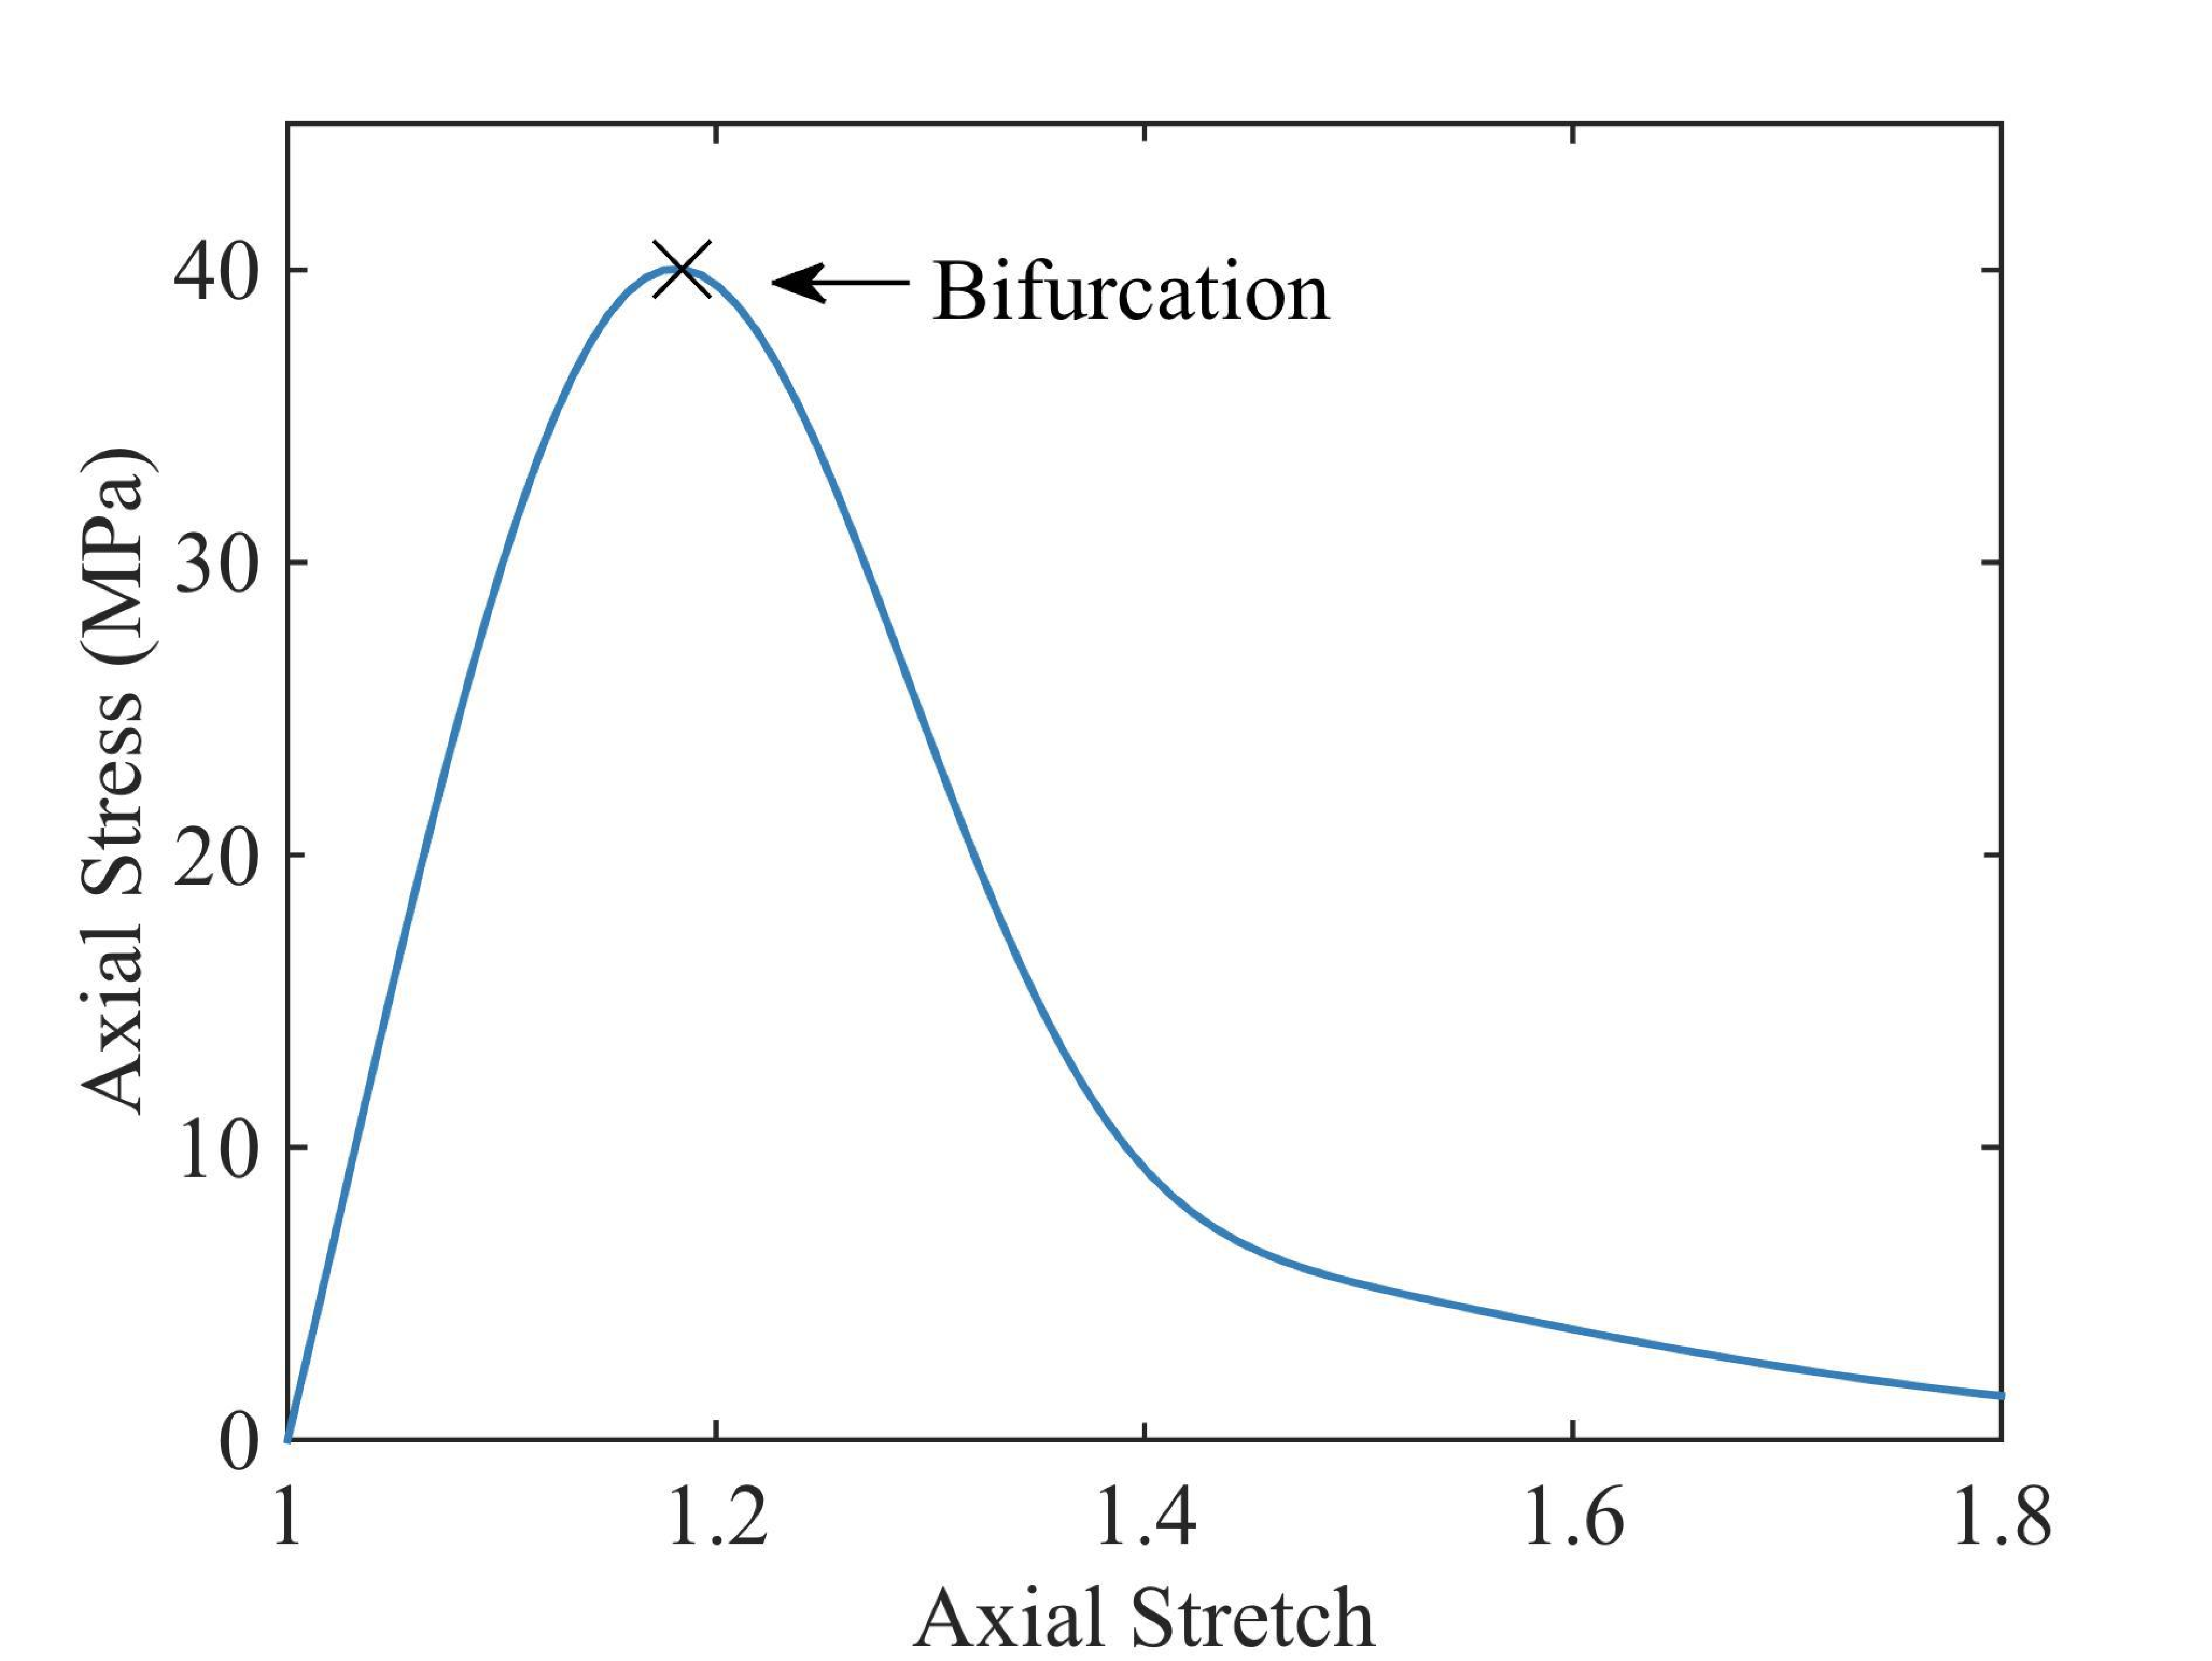
\includegraphics[width=0.45\textwidth]
    {figs/aniso_uniaxial_stress_stretch.pdf}
  } \subfigure[]{
    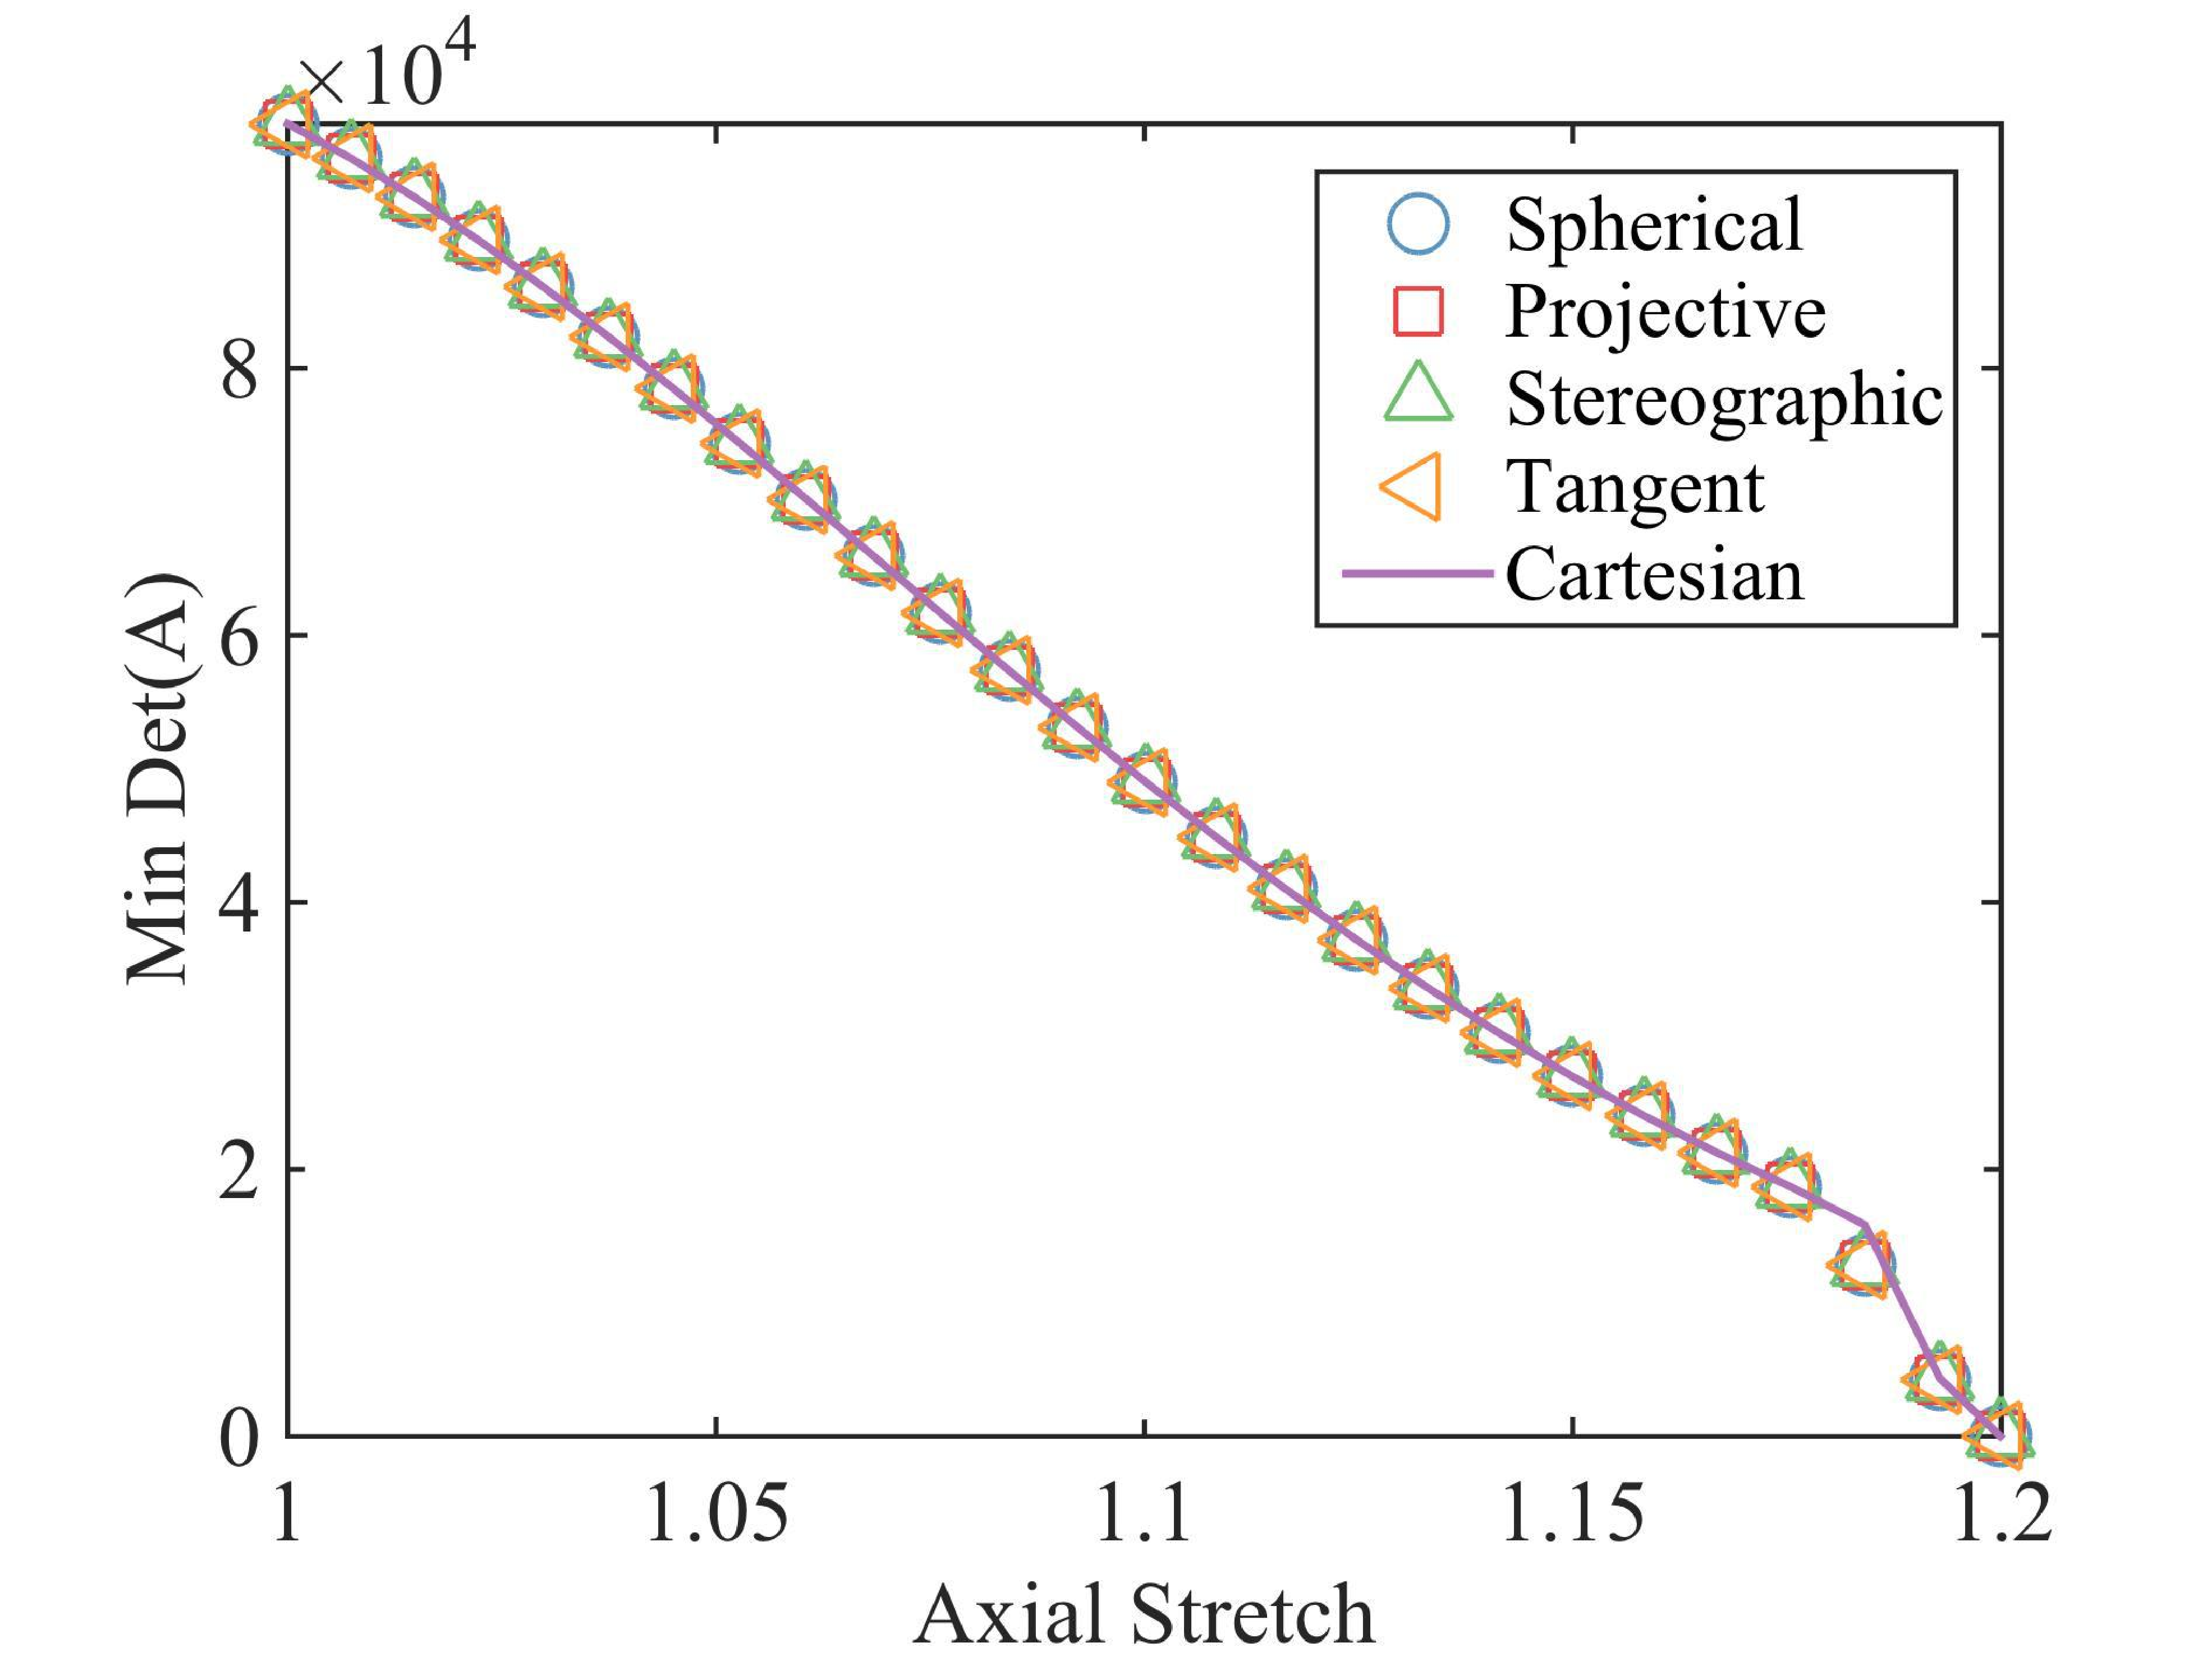
\includegraphics[width=0.45\textwidth]
    {figs/aniso_uniaxial_mindetA_stretch.pdf}
  }
  \caption{Uniaxial tension test on finite deformation 
  anisotropic damage model: 
  (a)stress strain behavior, with the cross indicating bifurcation, and
  (b) degradation of det$\bA$ for different
  parametrizations.}
  \label{fig:aniso_stress_stretch}
\end{figure}

As in the previous example, the computational cost of different 
parametrizations at the loading increment leading to bifurcation is 
recorded and shown in Table~\ref{tab:aniso_uniaxial_runtime}. Again, 
the density of the initial sampling is represented by the sampling 
interval and the number of sampling points. In general, as the number 
of sampling points decreases, so does the computational cost. However, 
the fewer sampling points may lead to a poor initial guess for the 
Newton iterative solve, which may cost more time to arrive at a 
converged solution. Because of the added complexity of the material 
model, different parametrizations are more sensitive to the density of 
the initial sampling grids. The spherical parametrization fails to 
correctly detect the bifurcation when the sampling interval is greater 
than 0.4. The stereographic, projective and tangent parametrizations, 
though more robust in this case, are computationally more expensive. 
The Cartesian parametrization is computationally efficient and at the 
same time, relatively insensitive to the sampling interval. 

\begin{table}[H]
  \begin{center}
    %\begin{tabular}{ p{1.5cm} | p{1.7cm} p{1.7cm} p{1.7cm} p{1.7cm} p{1.7cm} }
    \begin{tabular}{c c | r r r r r}
      \toprule
      Sampling   & Sampling &   \multicolumn{5}{c}{Run time ($\mu$s)}	\\   
      interval     & points     &  Spherical    &   Stereographic  &   Projective  &   Tangent   & Cartesian  \\
      \midrule         
      0.05      &      41     &      396     &    254       &       5828       &       330        &      412           \\
      0.1        &      21     &      242     &    207       &       926         &       212        &      214           \\
      0.2        &      11     &      188     &    181       &       296         &       187        &      122           \\
      0.3        &      7       &      207     &    210       &       250         &       187        &      132           \\
      0.4        &      5       &      169     &    208       &       268         &       189        &      111           \\       
      0.5        &      5       &	  167     &    n/a        &       239         &       n/a         &      123           \\
      0.6        &      3       &	  201     &    173       &       228         &       215        &      281           \\
      0.7        &      3       &	  n/a      &    175 	     &       193         &       157        &      141           \\
      0.8        &      3       &      n/a      &    213       &       187         &       183        &       101          \\	      
      0.9        &      3       &	  n/a      &    214       &       225         &       204        &       99            \\	
      1.0        &      3       &      n/a      &    n/a	     &       225         &       n/a         &       118          \\	
      1.5        &      1       &	  n/a      &    n/a	     &       n/a          &       n/a         &       n/a           \\	       
      \bottomrule
    \end{tabular}
    \caption{Computational cost of different parametrizations in 
    uniaxial tension test at loading increment leading to bifurcation. 
    `n/a' means the parametrization fails to detect bifurcation in 
    this loading increment.}
    \label{tab:aniso_uniaxial_runtime}
  \end{center}
\end{table}

To gain insights into the influence of parametrizations on the 
determinant function det$\bA$ as loading proceeds, we plot the 
landscapes at four different axial stretch levels for different 
parametrizations, as shown in Figures~\ref{fig:aniso_spherical_detA} - 
\ref{fig:aniso_cartesian_detA}.

\begin{figure}[H]
   \centering \subfigure[$F_{11}=1.0074$]{
   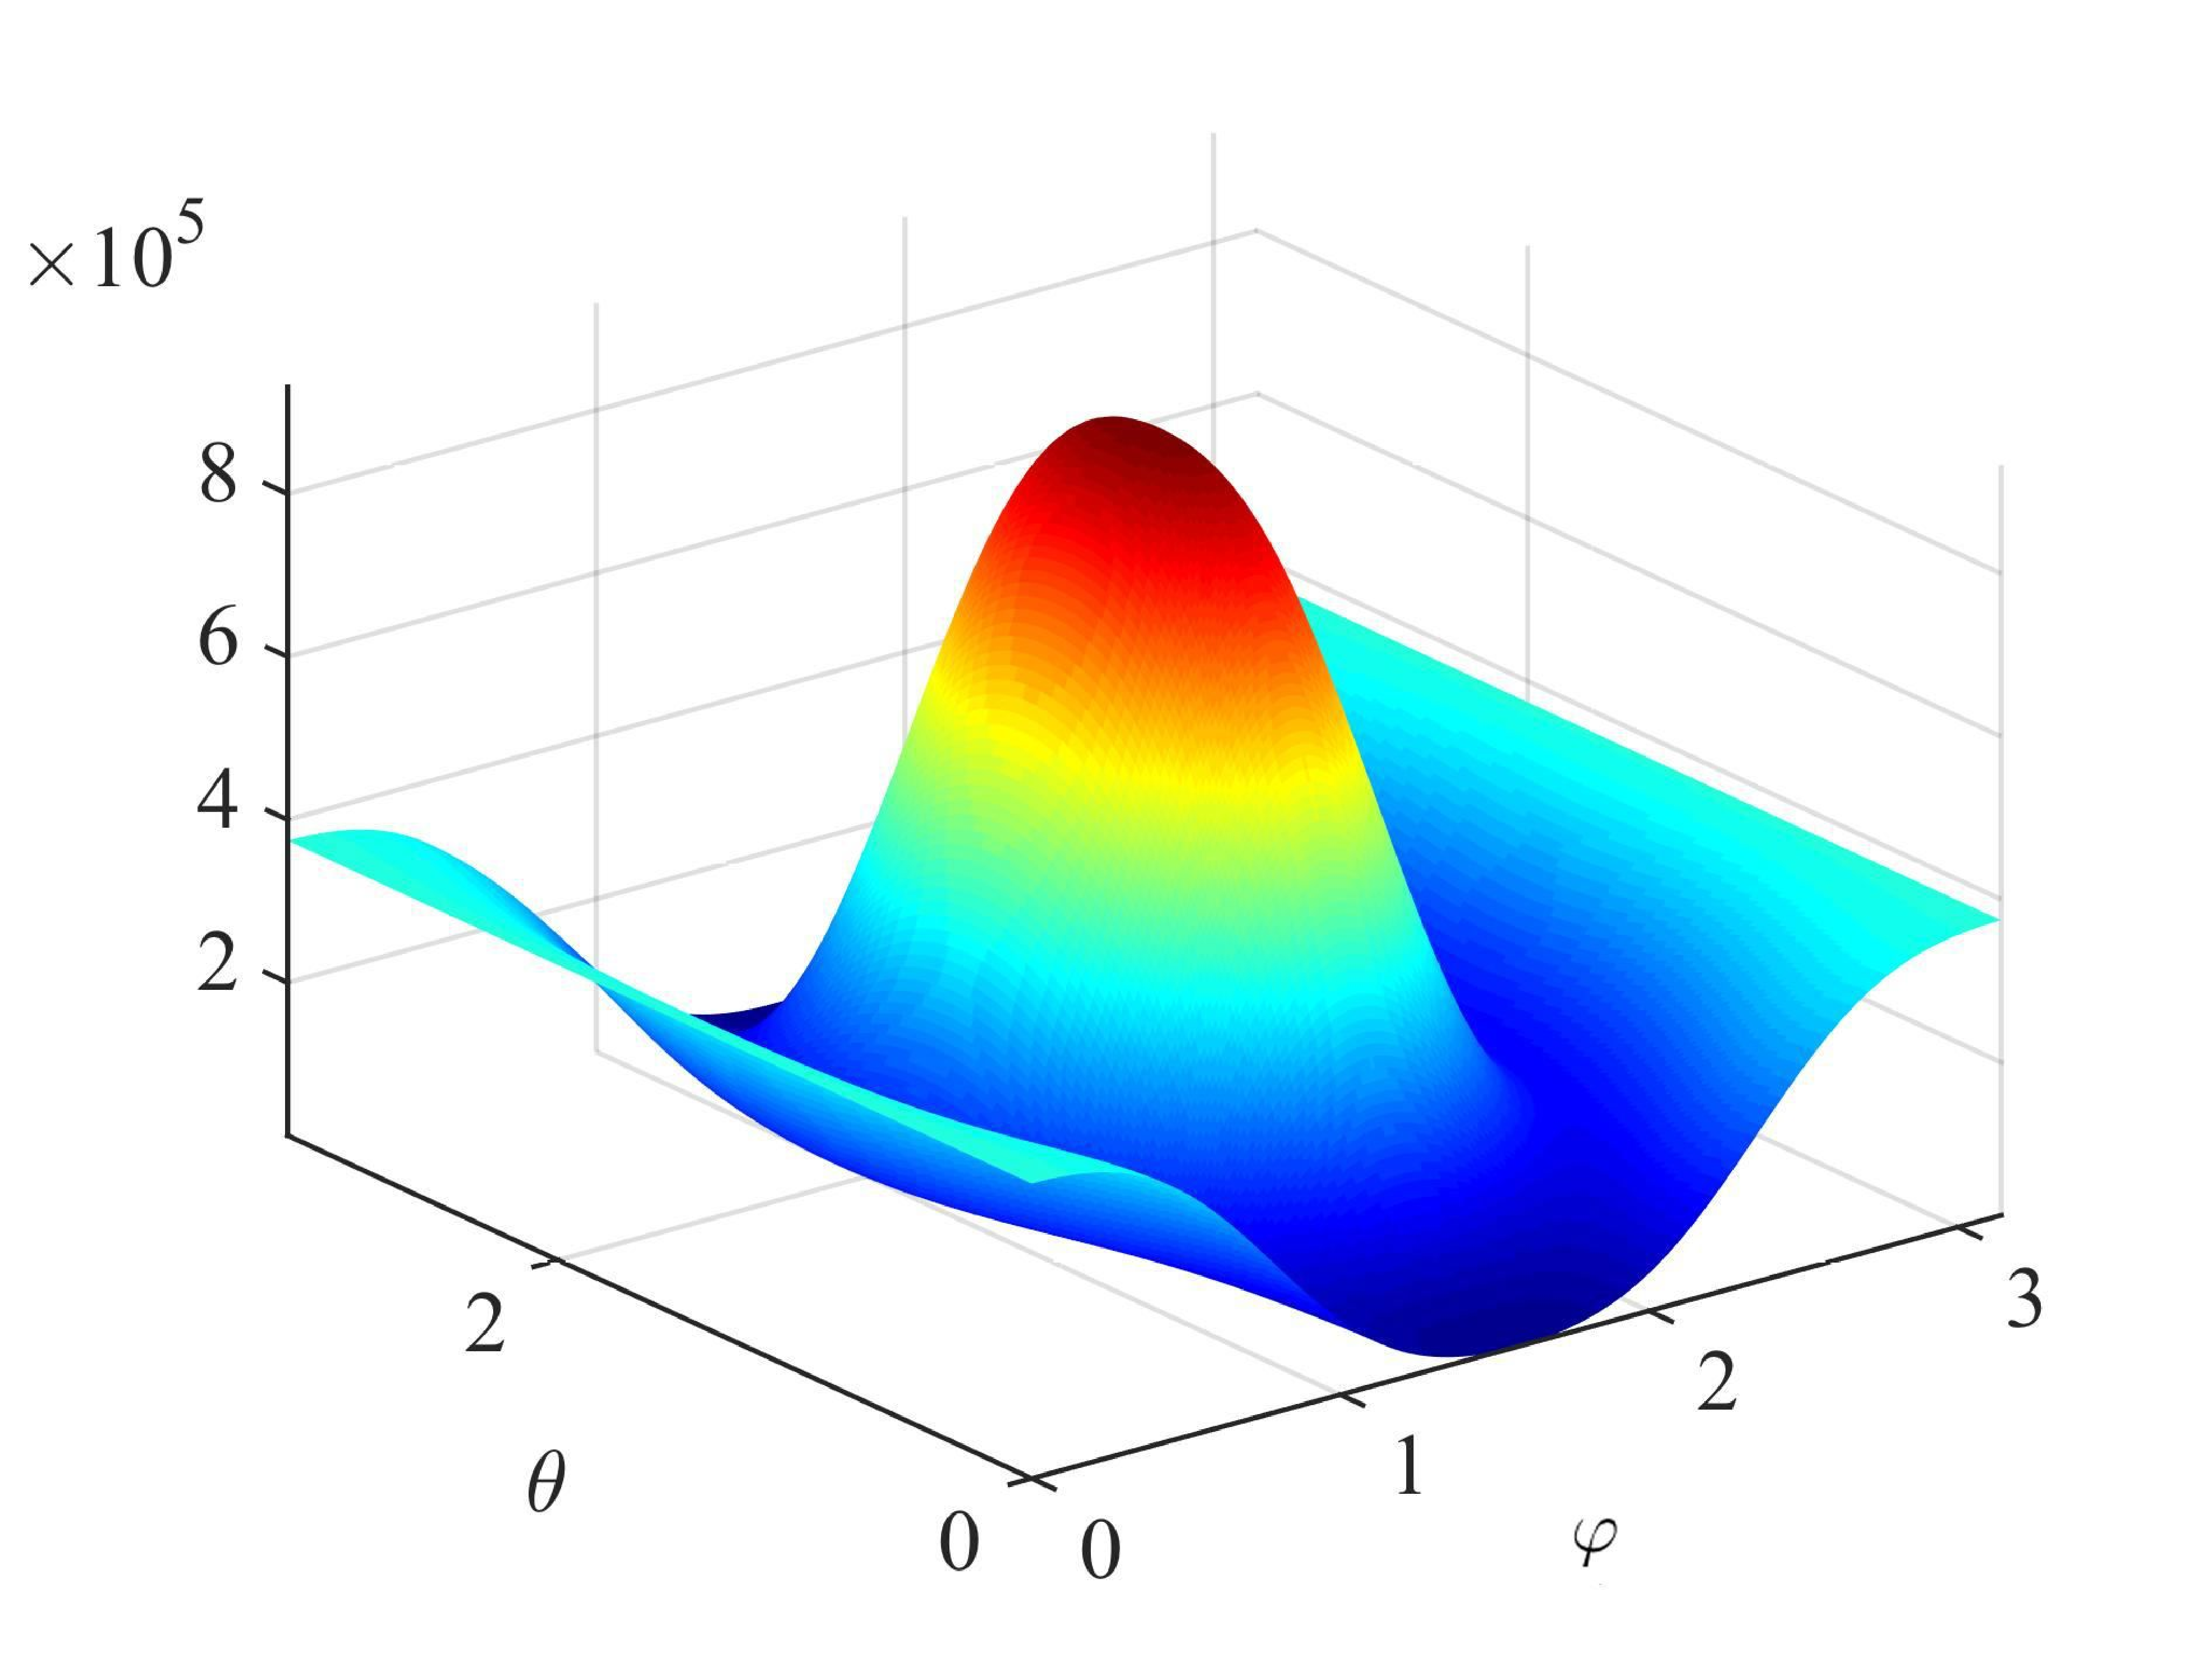
\includegraphics[width=0.45\textwidth]
   {figs/aniso_uniaxial_spherical_detA_F1p0074.pdf}
 } \subfigure[$F_{11}=1.0762$]{
   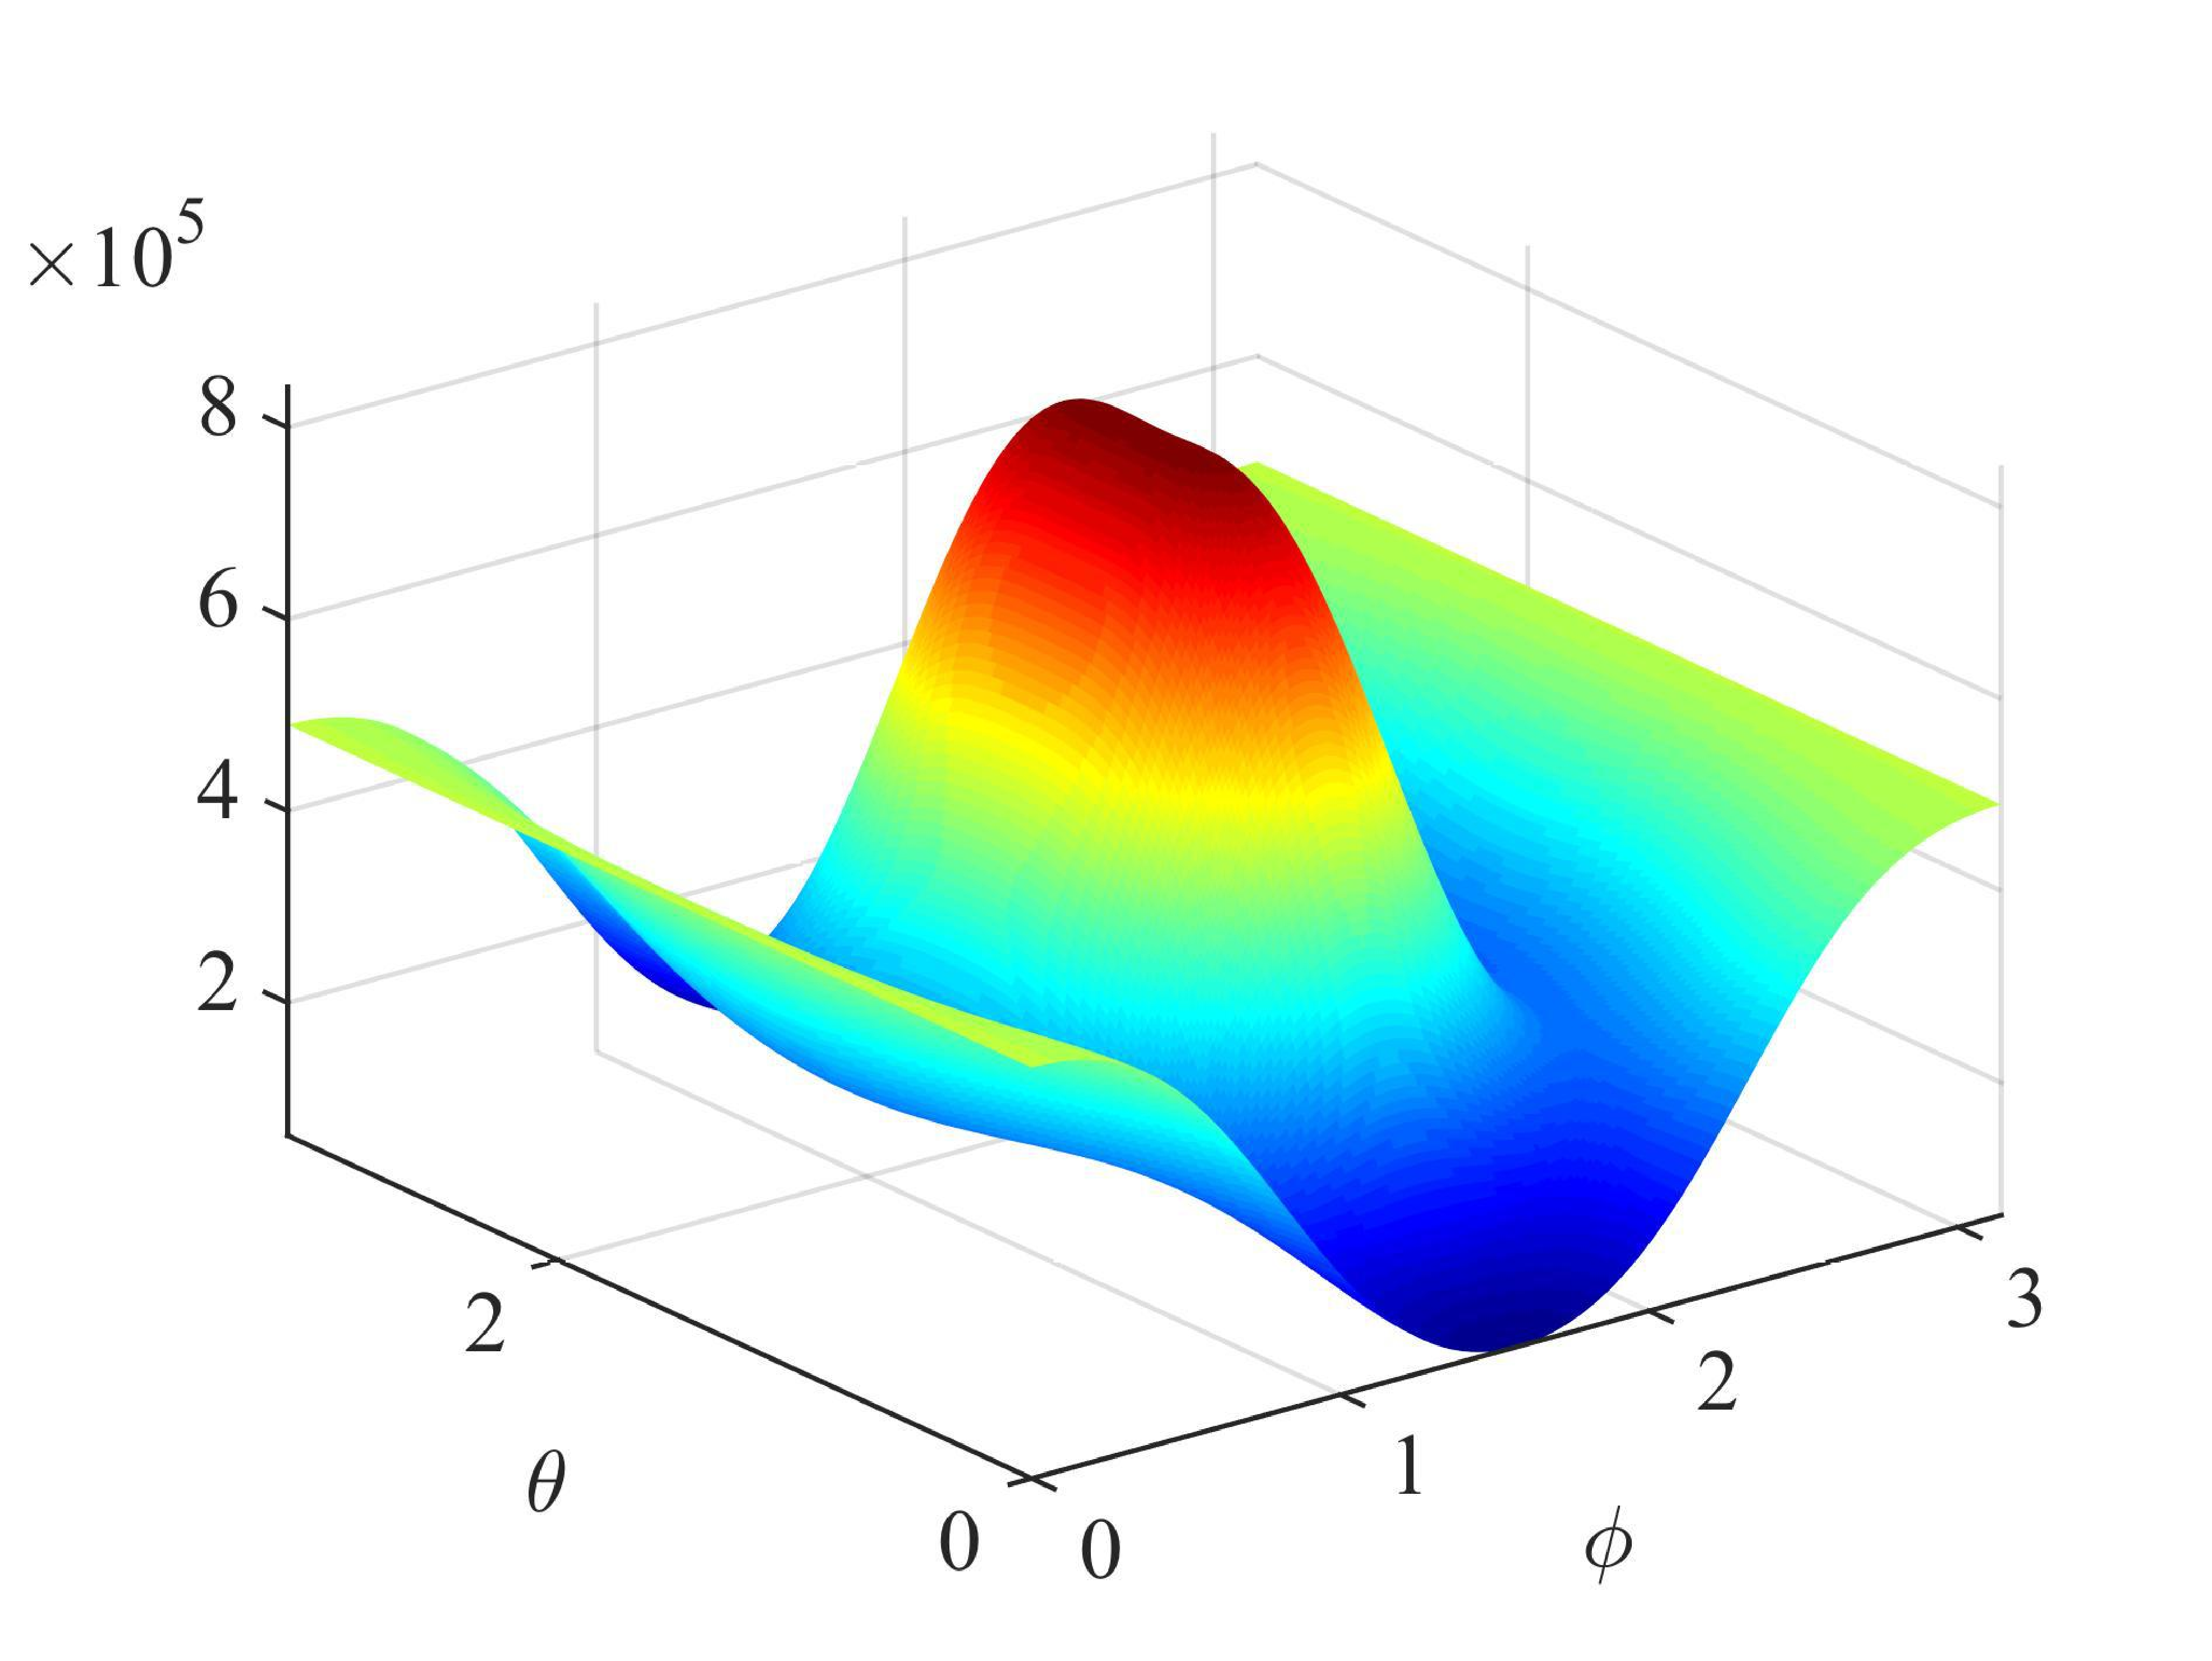
\includegraphics[width=0.45\textwidth]
   {figs/aniso_uniaxial_spherical_detA_F1p0762.pdf}
 } \subfigure[$F_{11}=1.1583$]{
   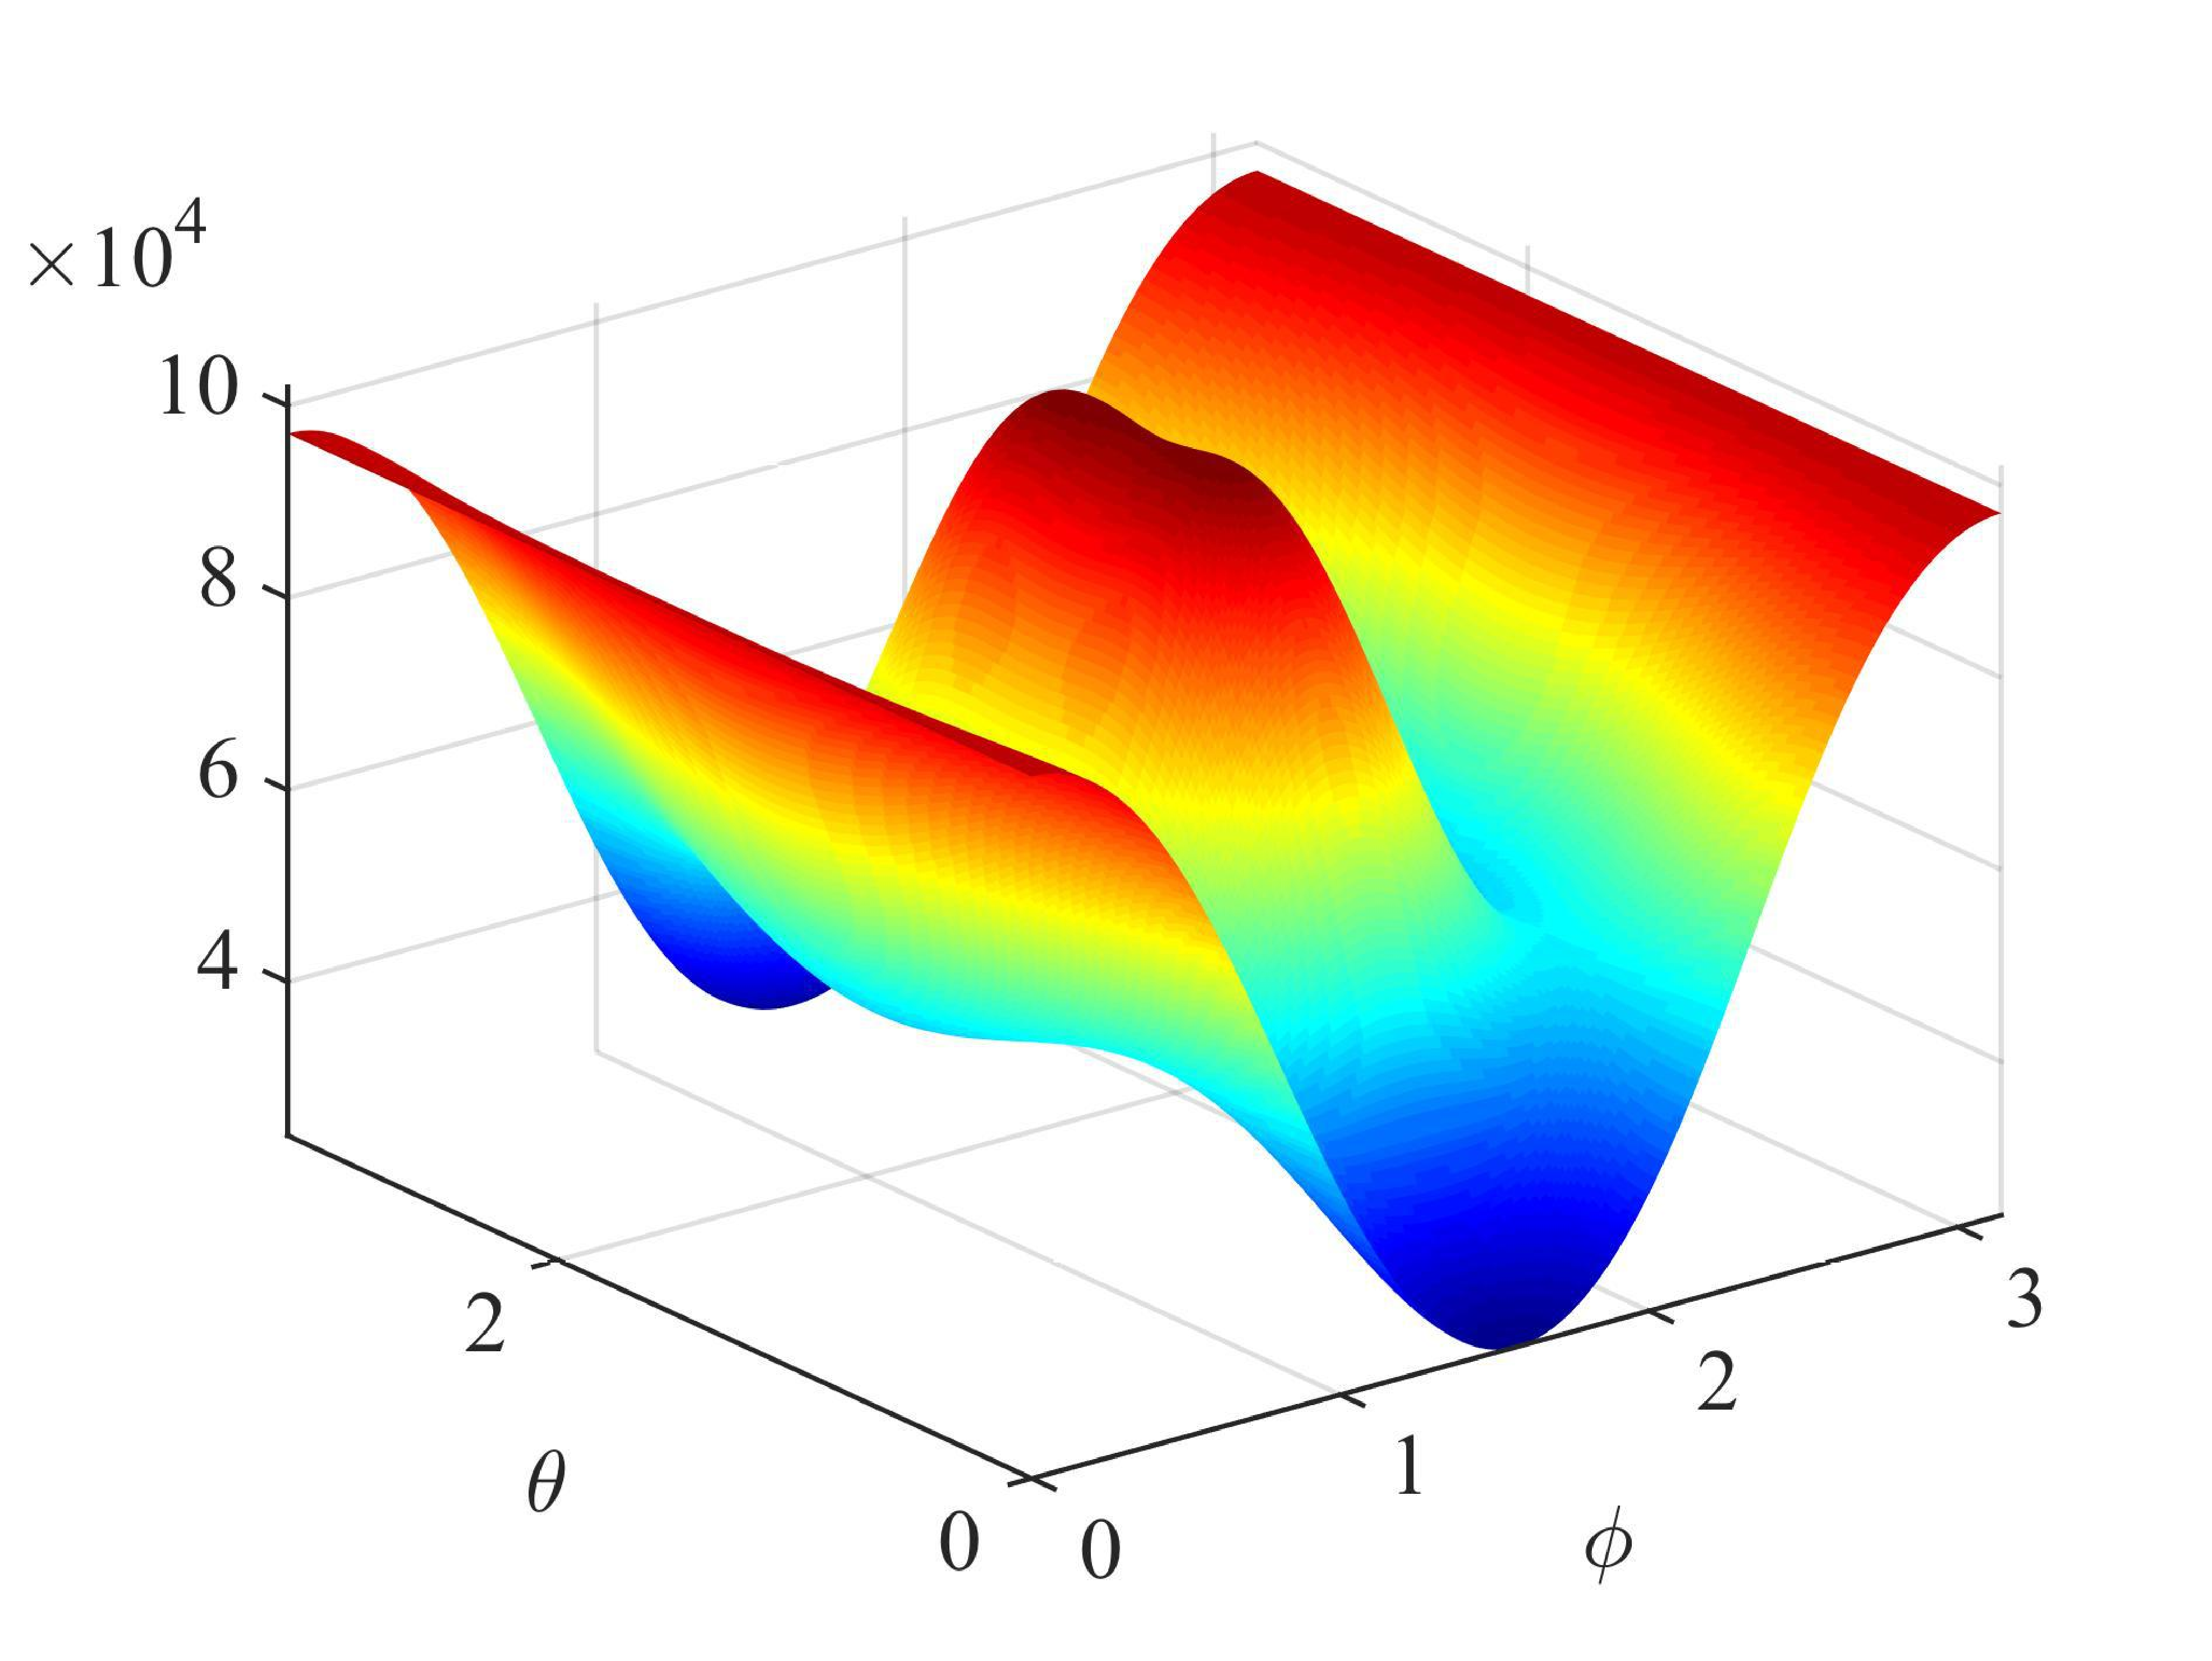
\includegraphics[width=0.45\textwidth]
   {figs/aniso_uniaxial_spherical_detA_F1p1583.pdf}
 } \subfigure[$F_{11}=1.1798$ (bifurcation)]{
   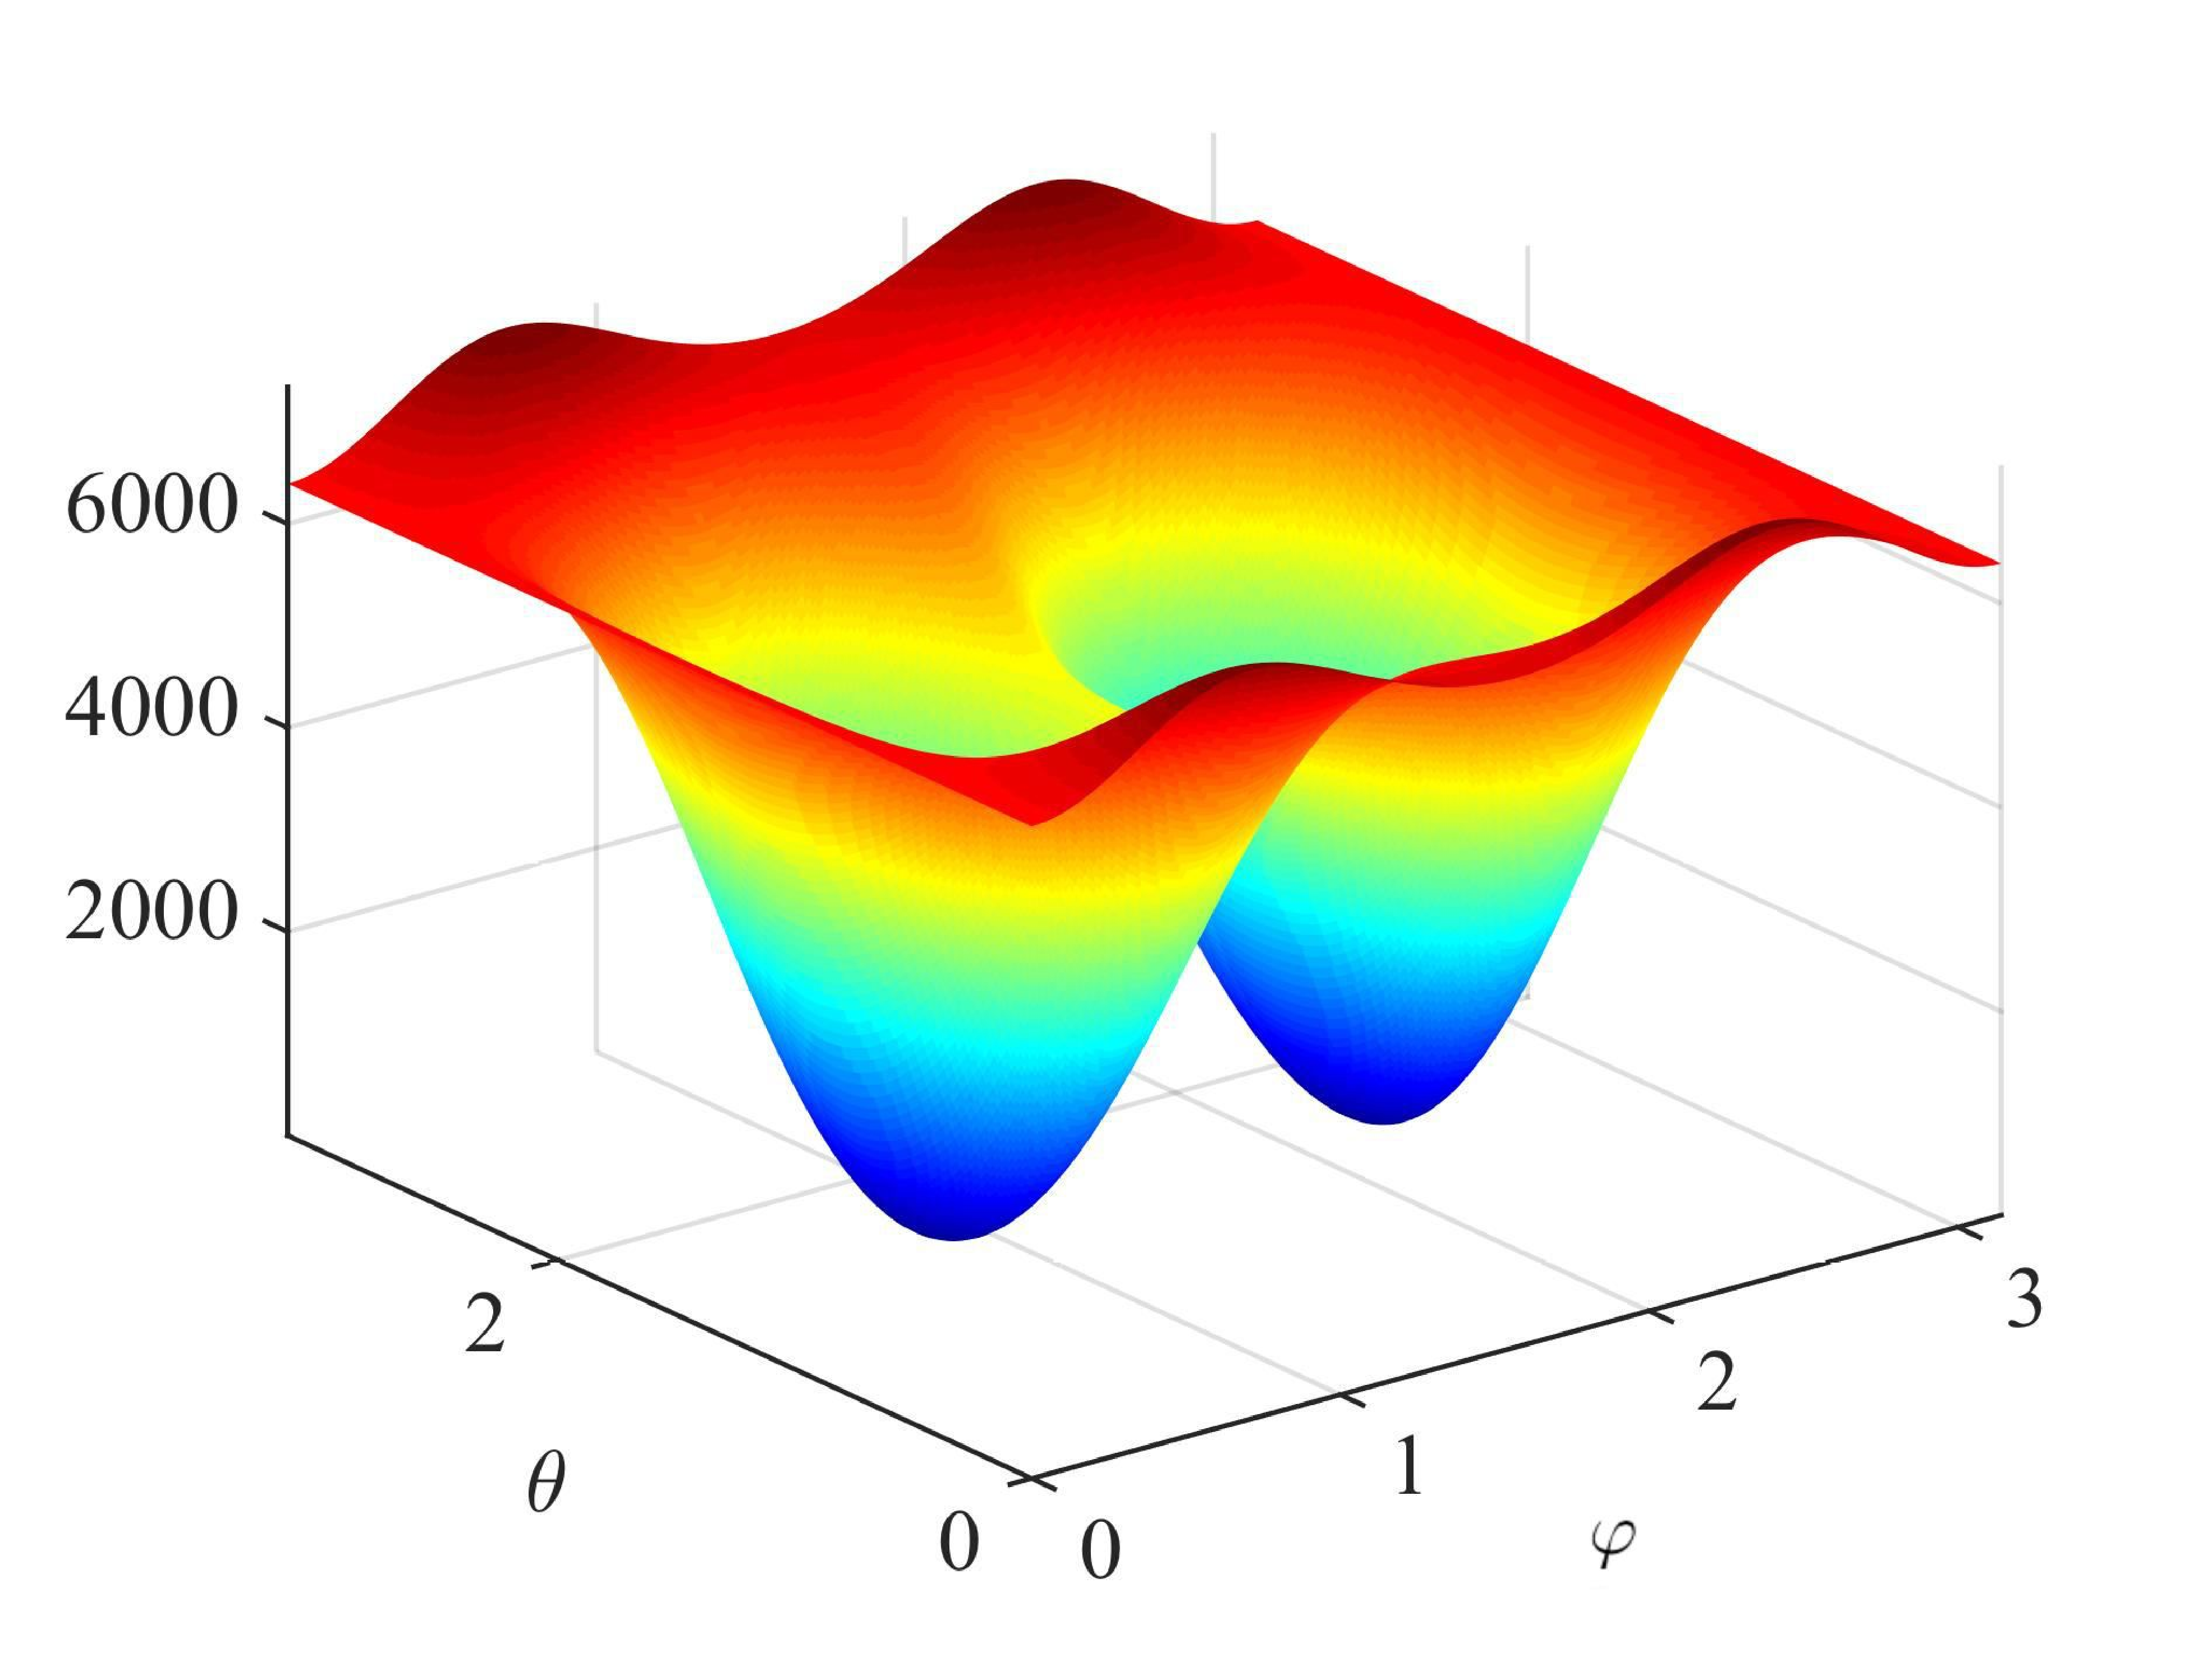
\includegraphics[width=0.45\textwidth]
   {figs/aniso_uniaxial_spherical_detA_F1p1798.pdf}
 }
   \caption{Spherical parametrization: landscapes of det$\bA$ 
   for uniaxial tension test on finite deformation anisotropic model at
   different axial stretch levels.}
   \label{fig:aniso_spherical_detA}
 \end{figure}

\begin{figure}[H]
   \centering \subfigure[$F_{11}=1.0074$]{
   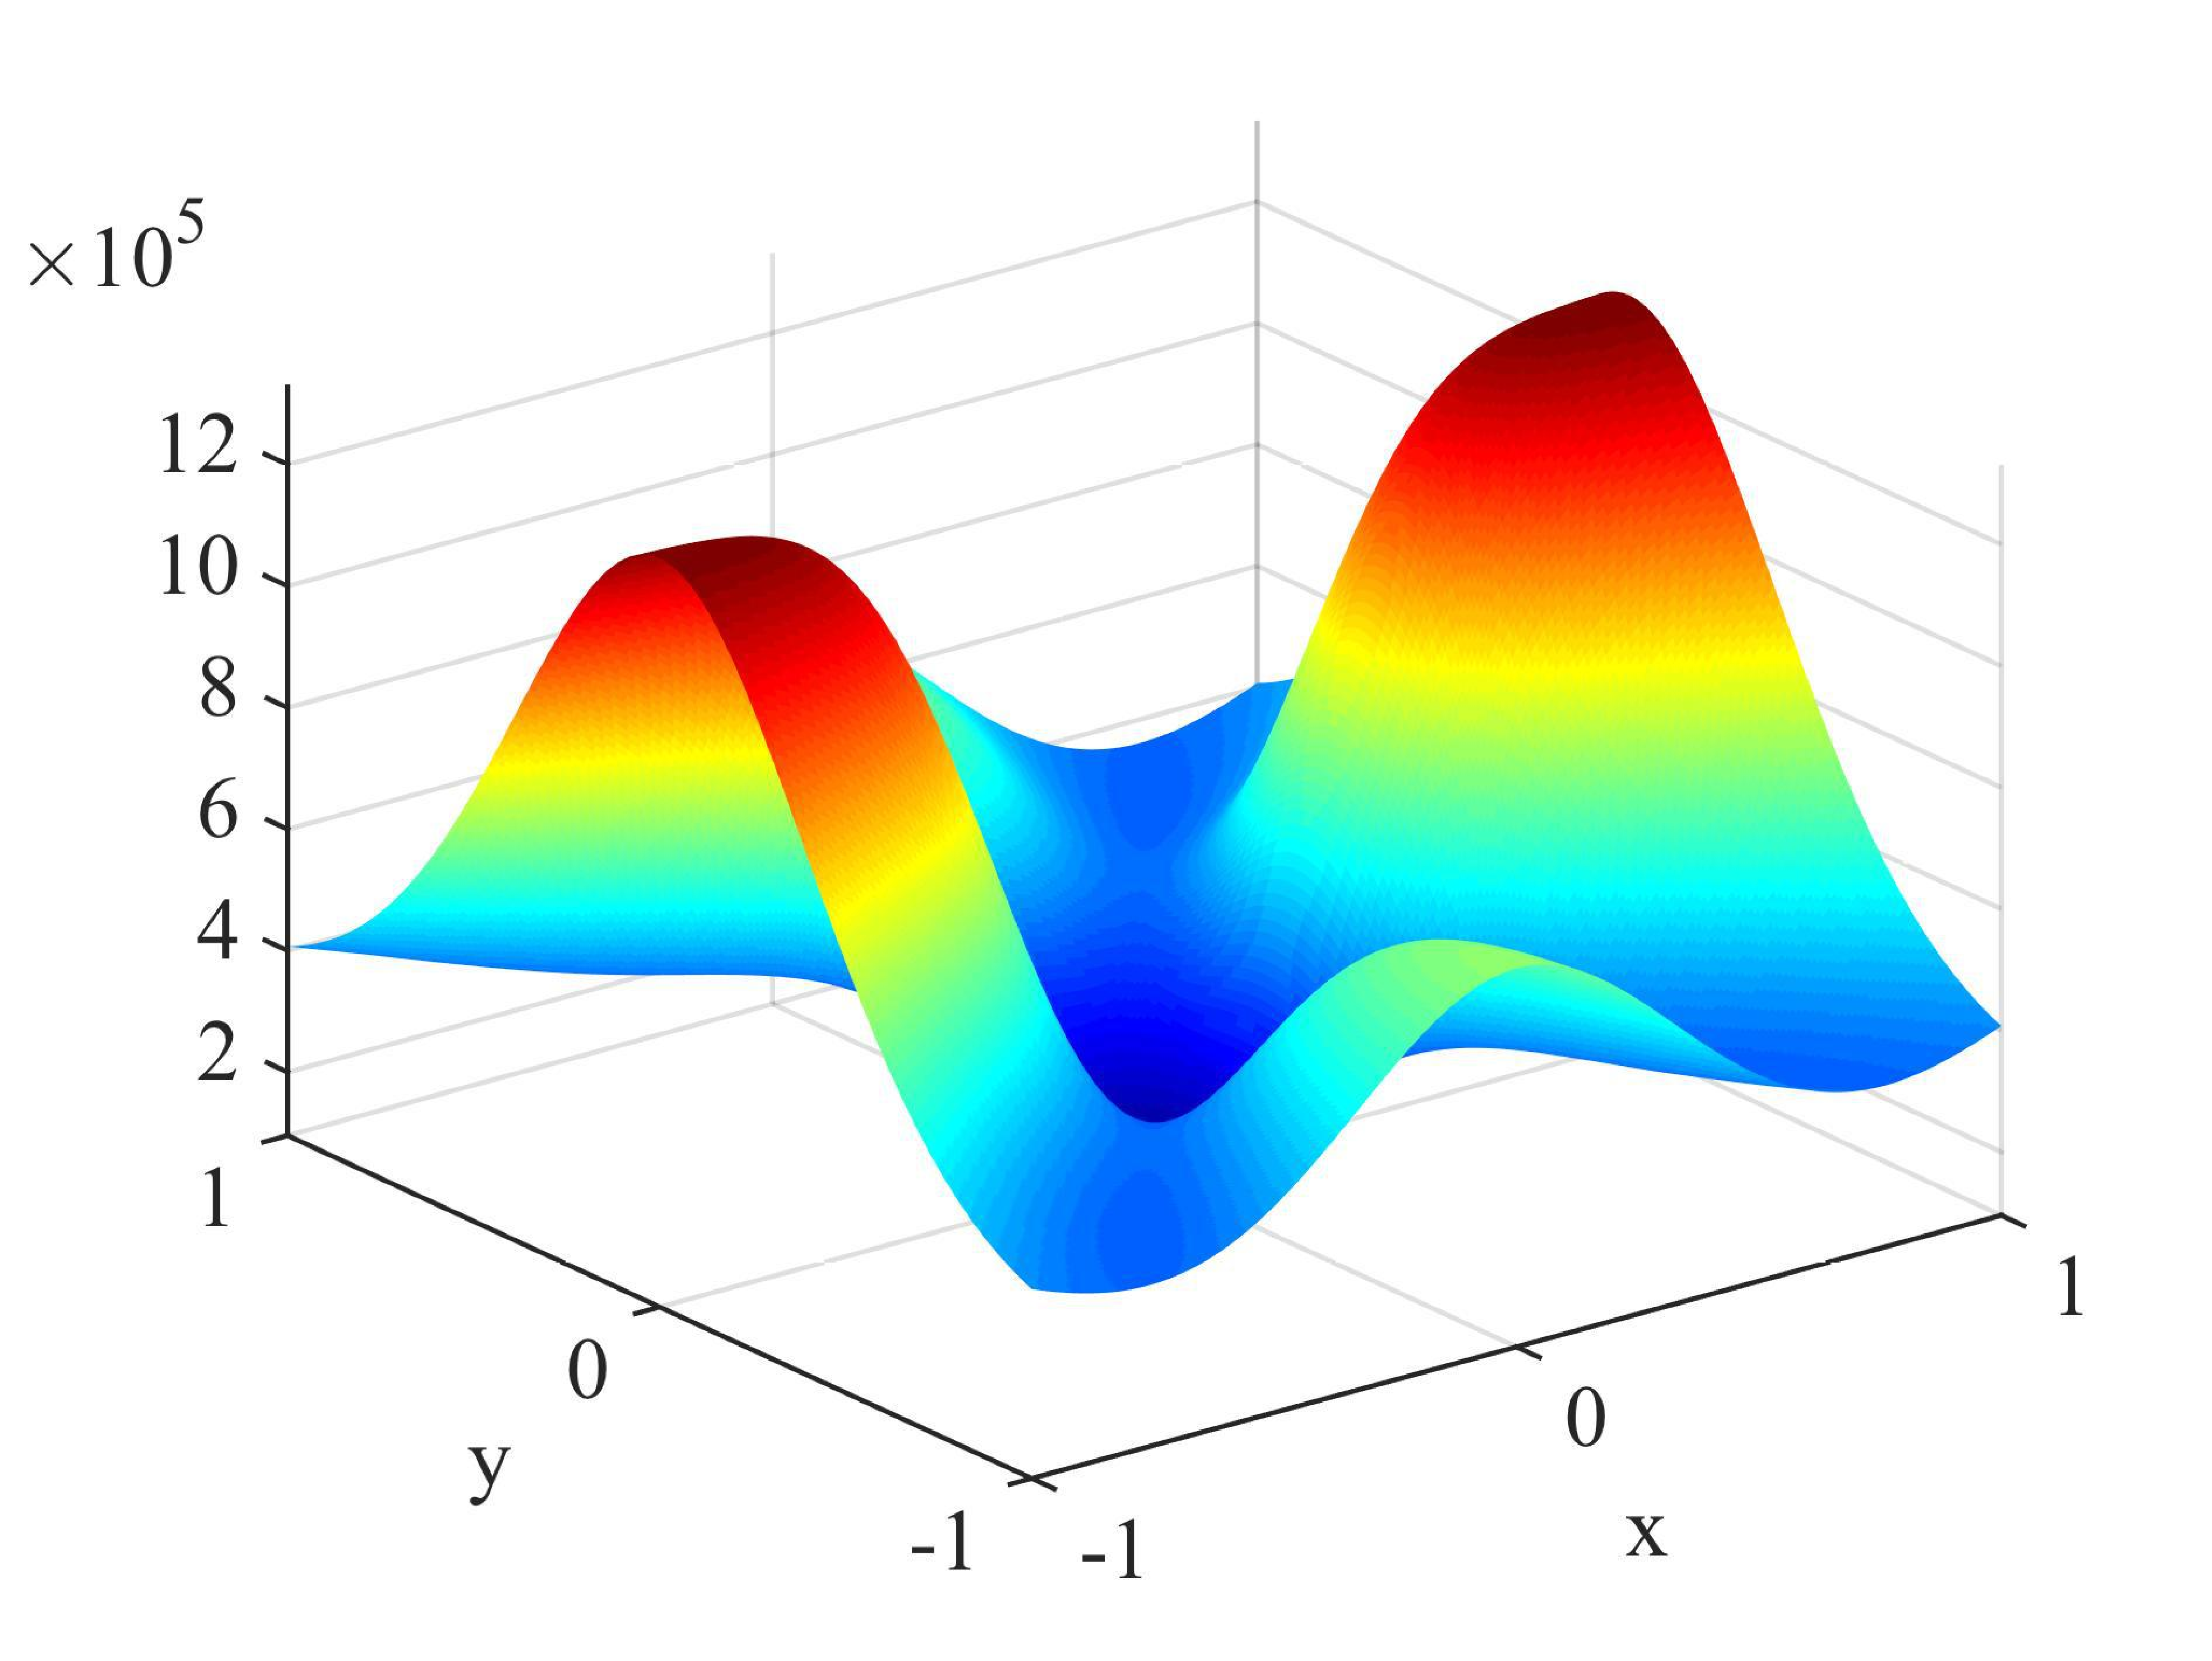
\includegraphics[width=0.45\textwidth]
   {figs/aniso_uniaxial_stereographic_detA_F1p0074.pdf}
 } \subfigure[$F_{11}=1.0762$]{
   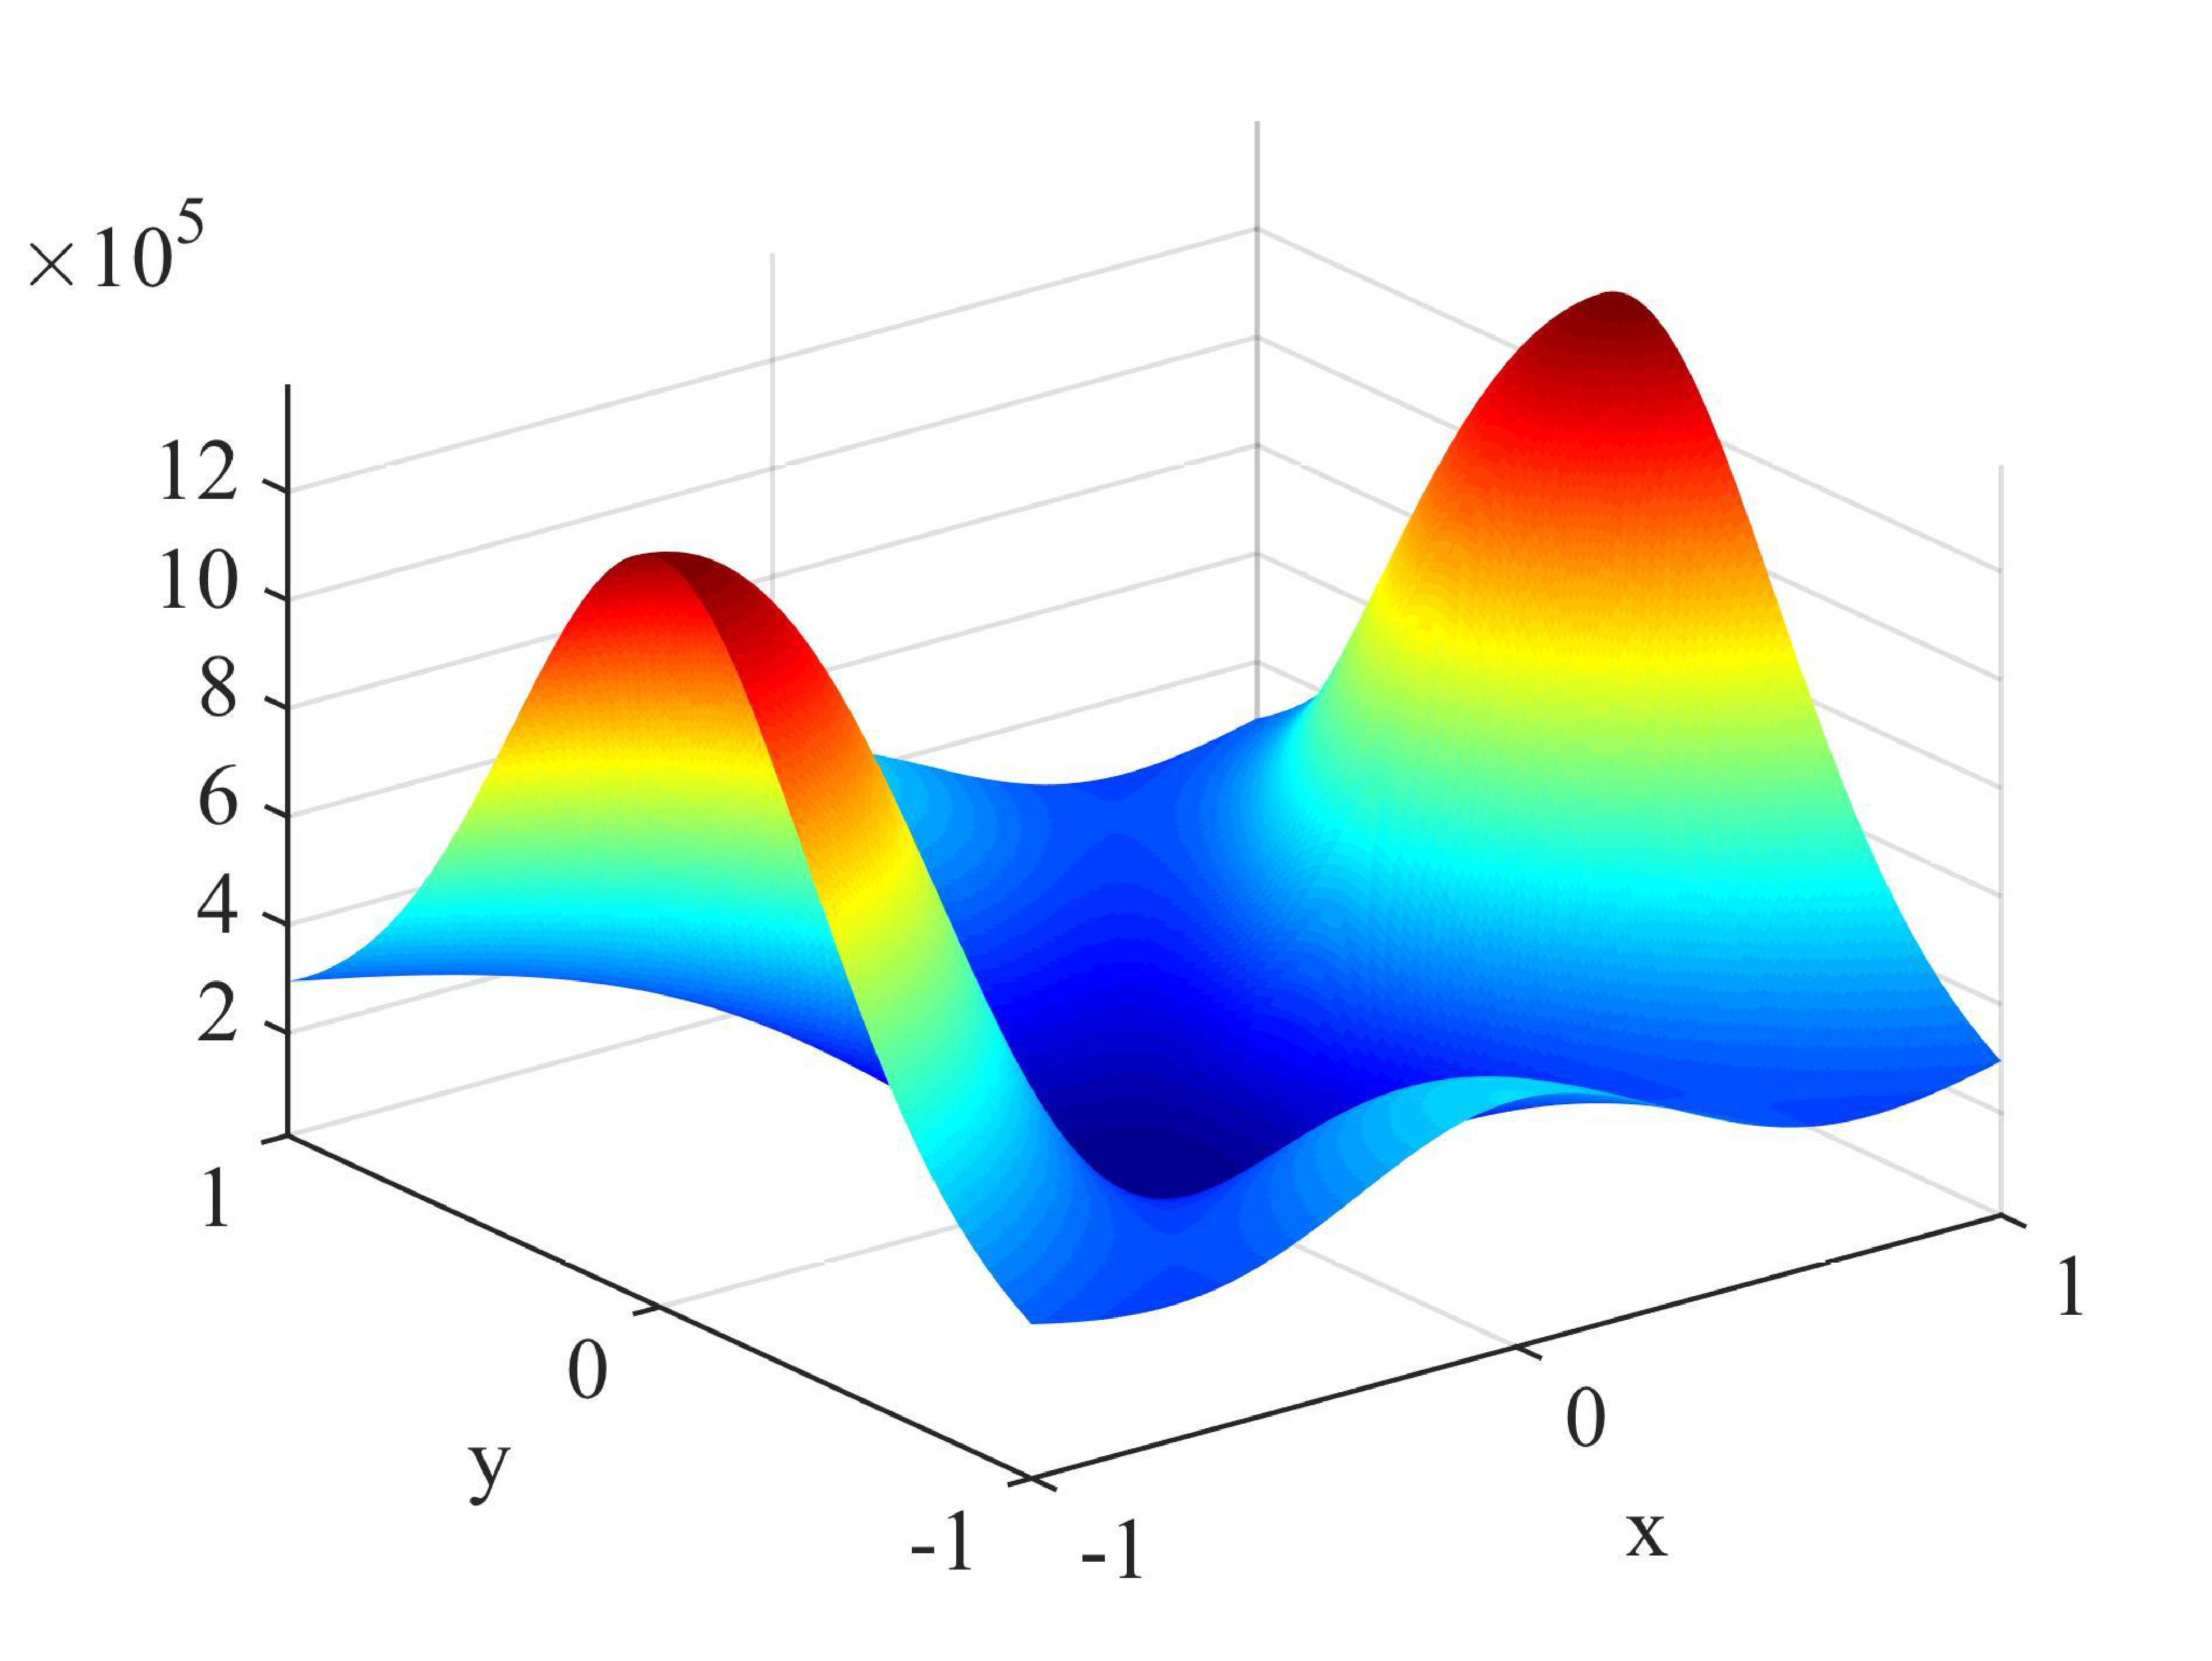
\includegraphics[width=0.45\textwidth]
   {figs/aniso_uniaxial_stereographic_detA_F1p0762.pdf}
 } \subfigure[$F_{11}=1.1583$]{
   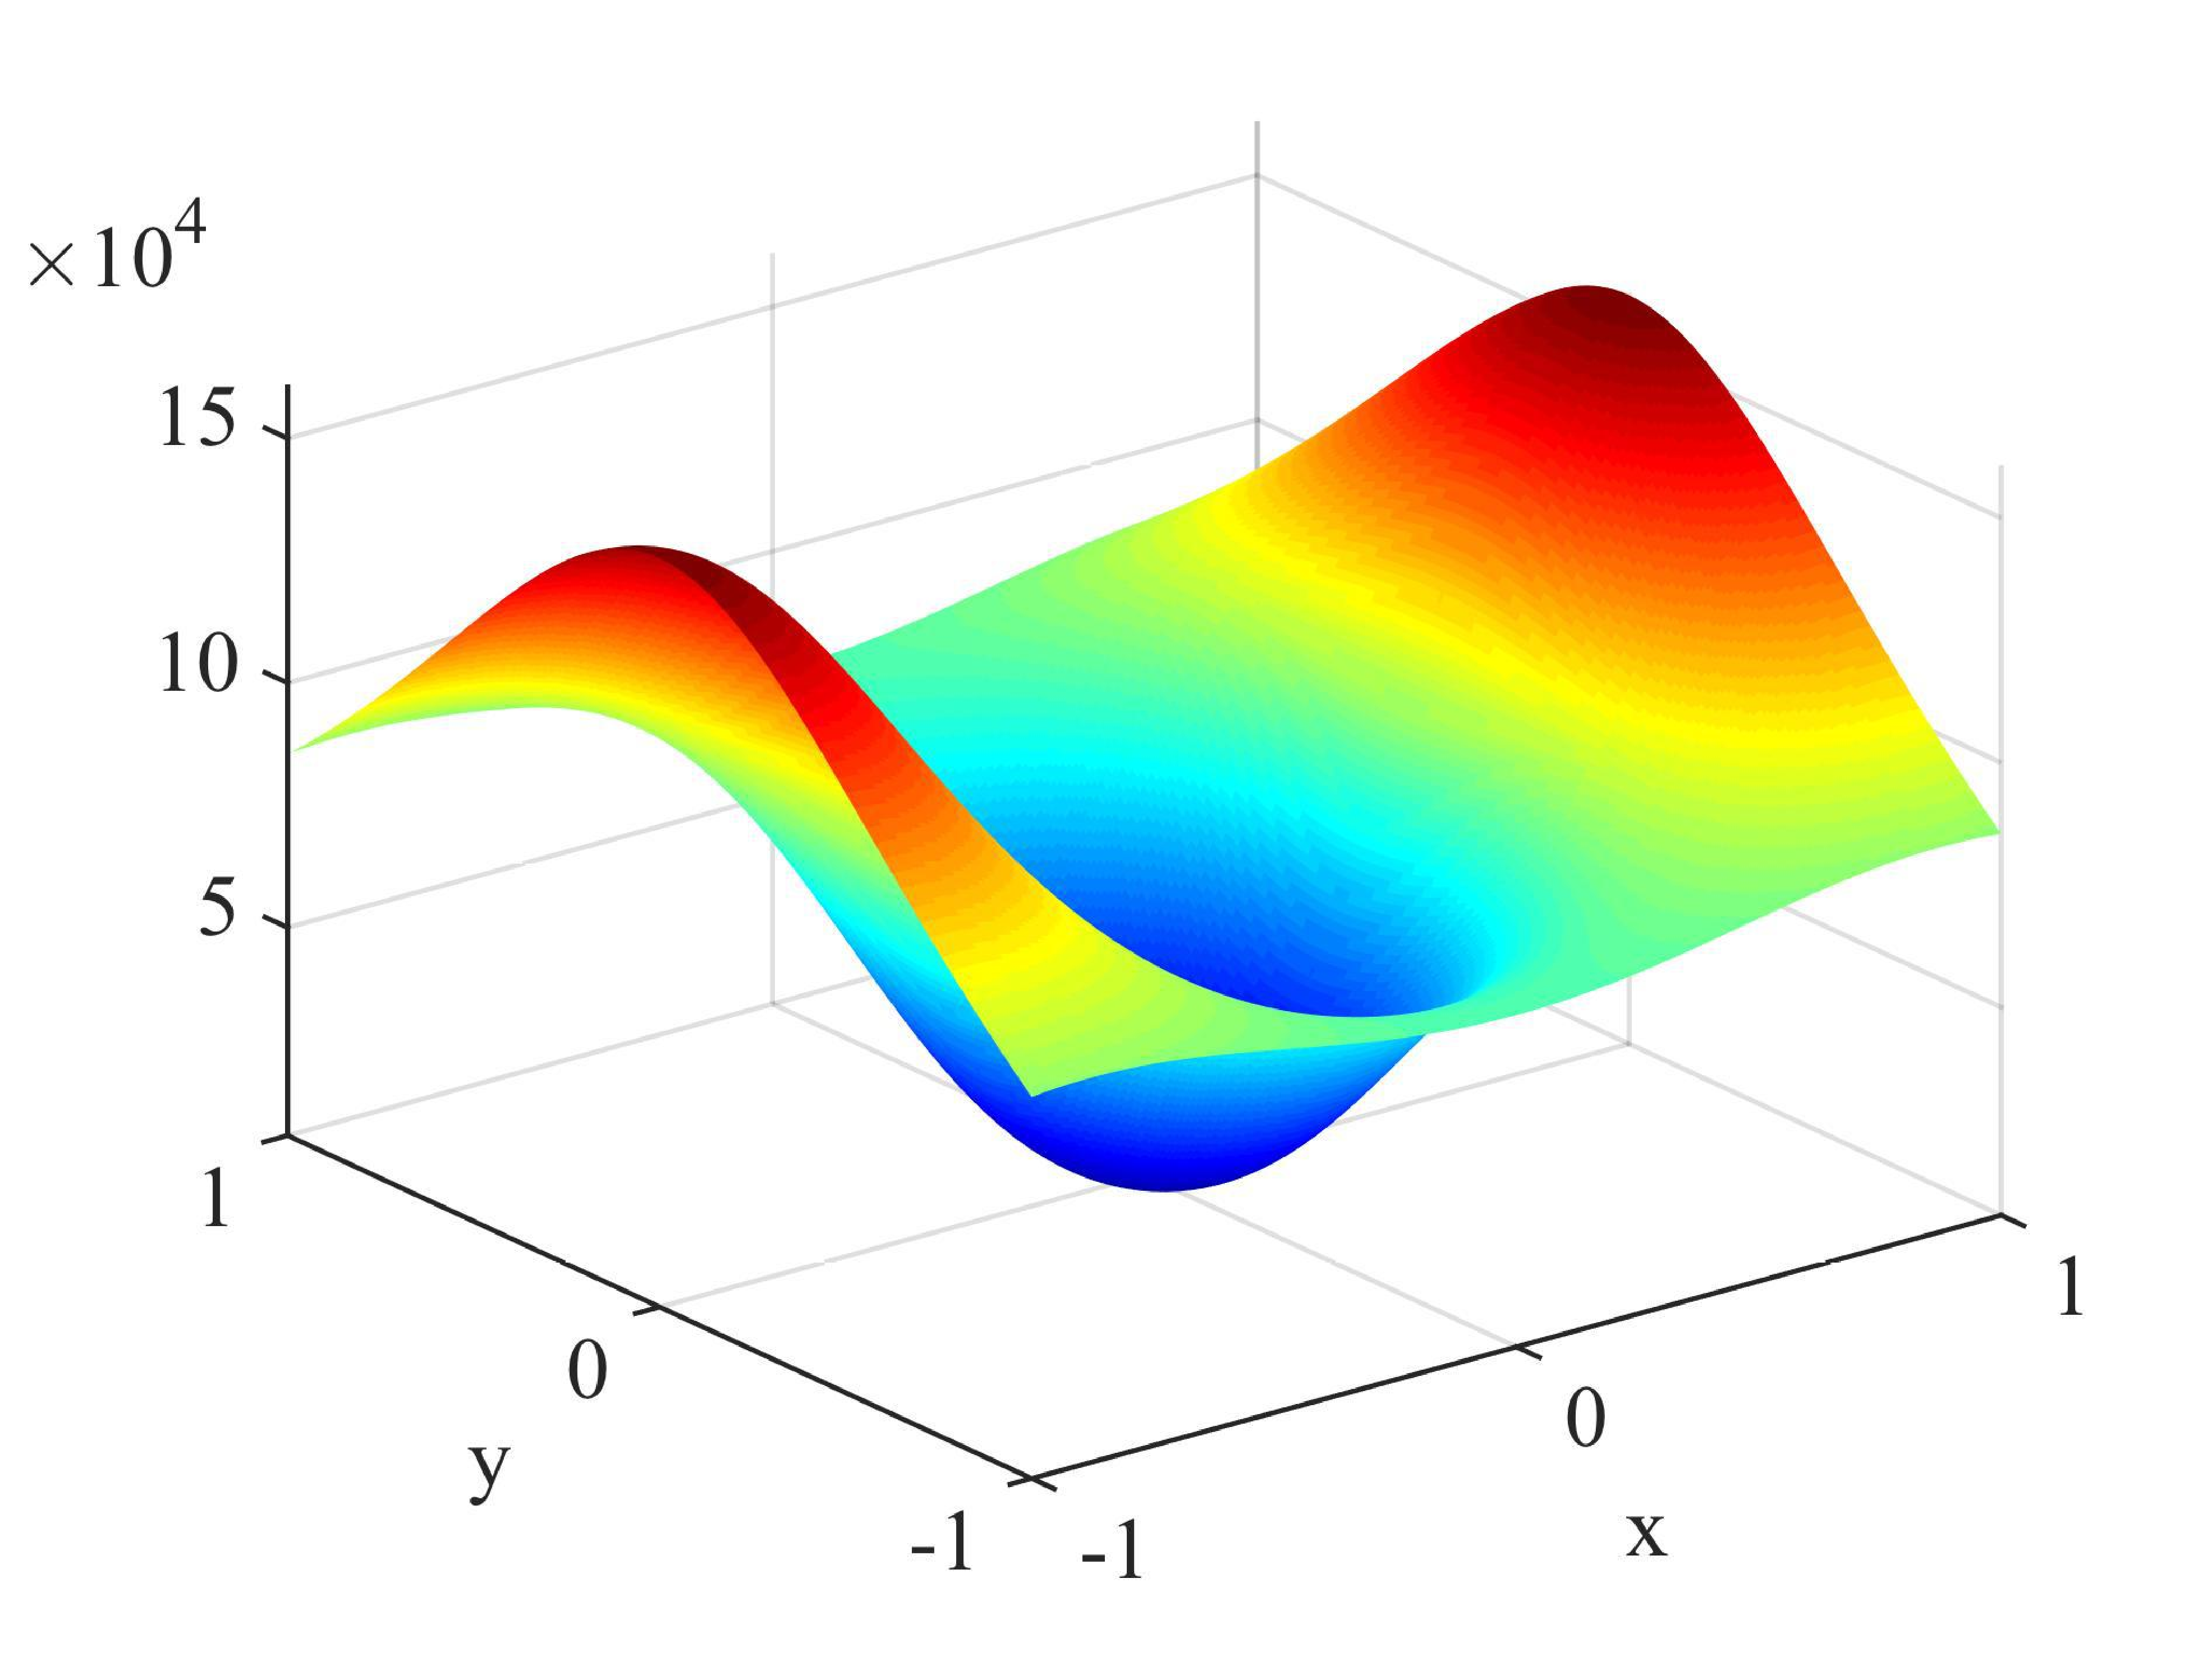
\includegraphics[width=0.45\textwidth]
   {figs/aniso_uniaxial_stereographic_detA_F1p1583.pdf}
 } \subfigure[$F_{11}=1.1798$ (bifurcation)]{
   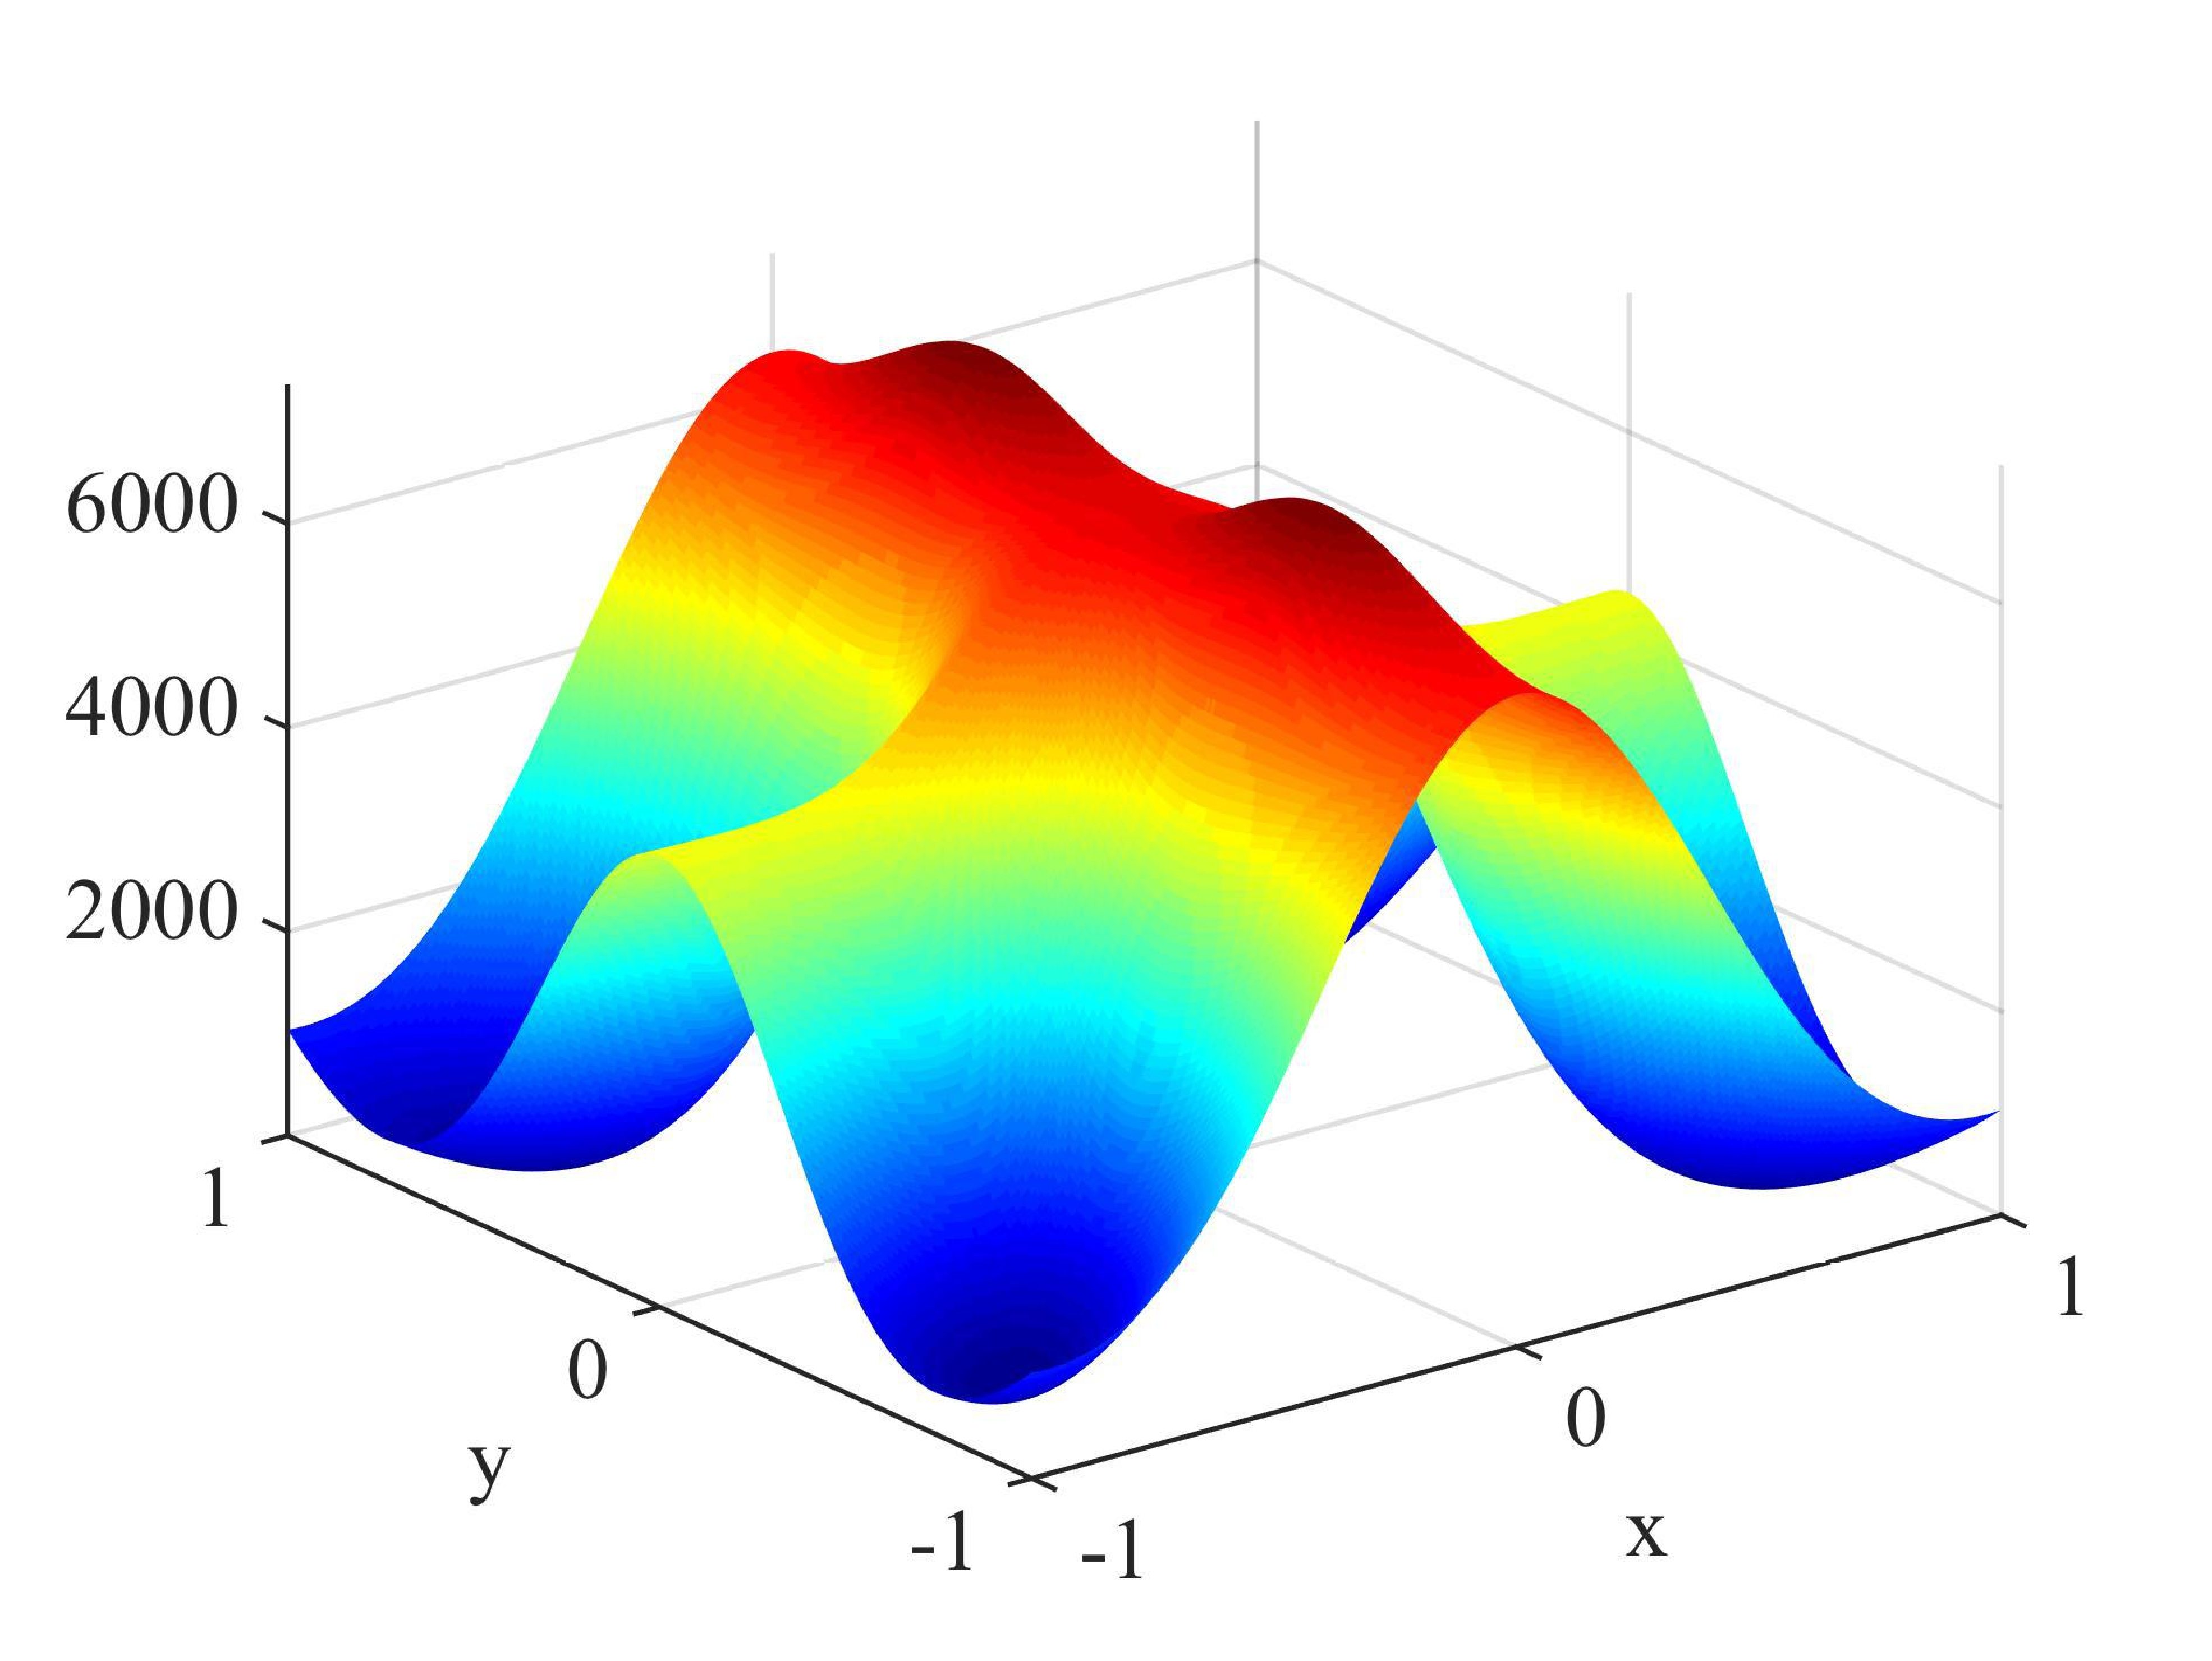
\includegraphics[width=0.45\textwidth]
   {figs/aniso_uniaxial_stereographic_detA_F1p1798.pdf}
 }
   \caption{Stereographic parametrization: landscapes of det$\bA$ 
   for uniaxial tension test on finite deformation anisotropic model at
   different axial stretch levels.}
   \label{fig:aniso_stereographic_detA}
 \end{figure}

\begin{figure}[H]
   \centering \subfigure[$F_{11}=1.0074$]{
   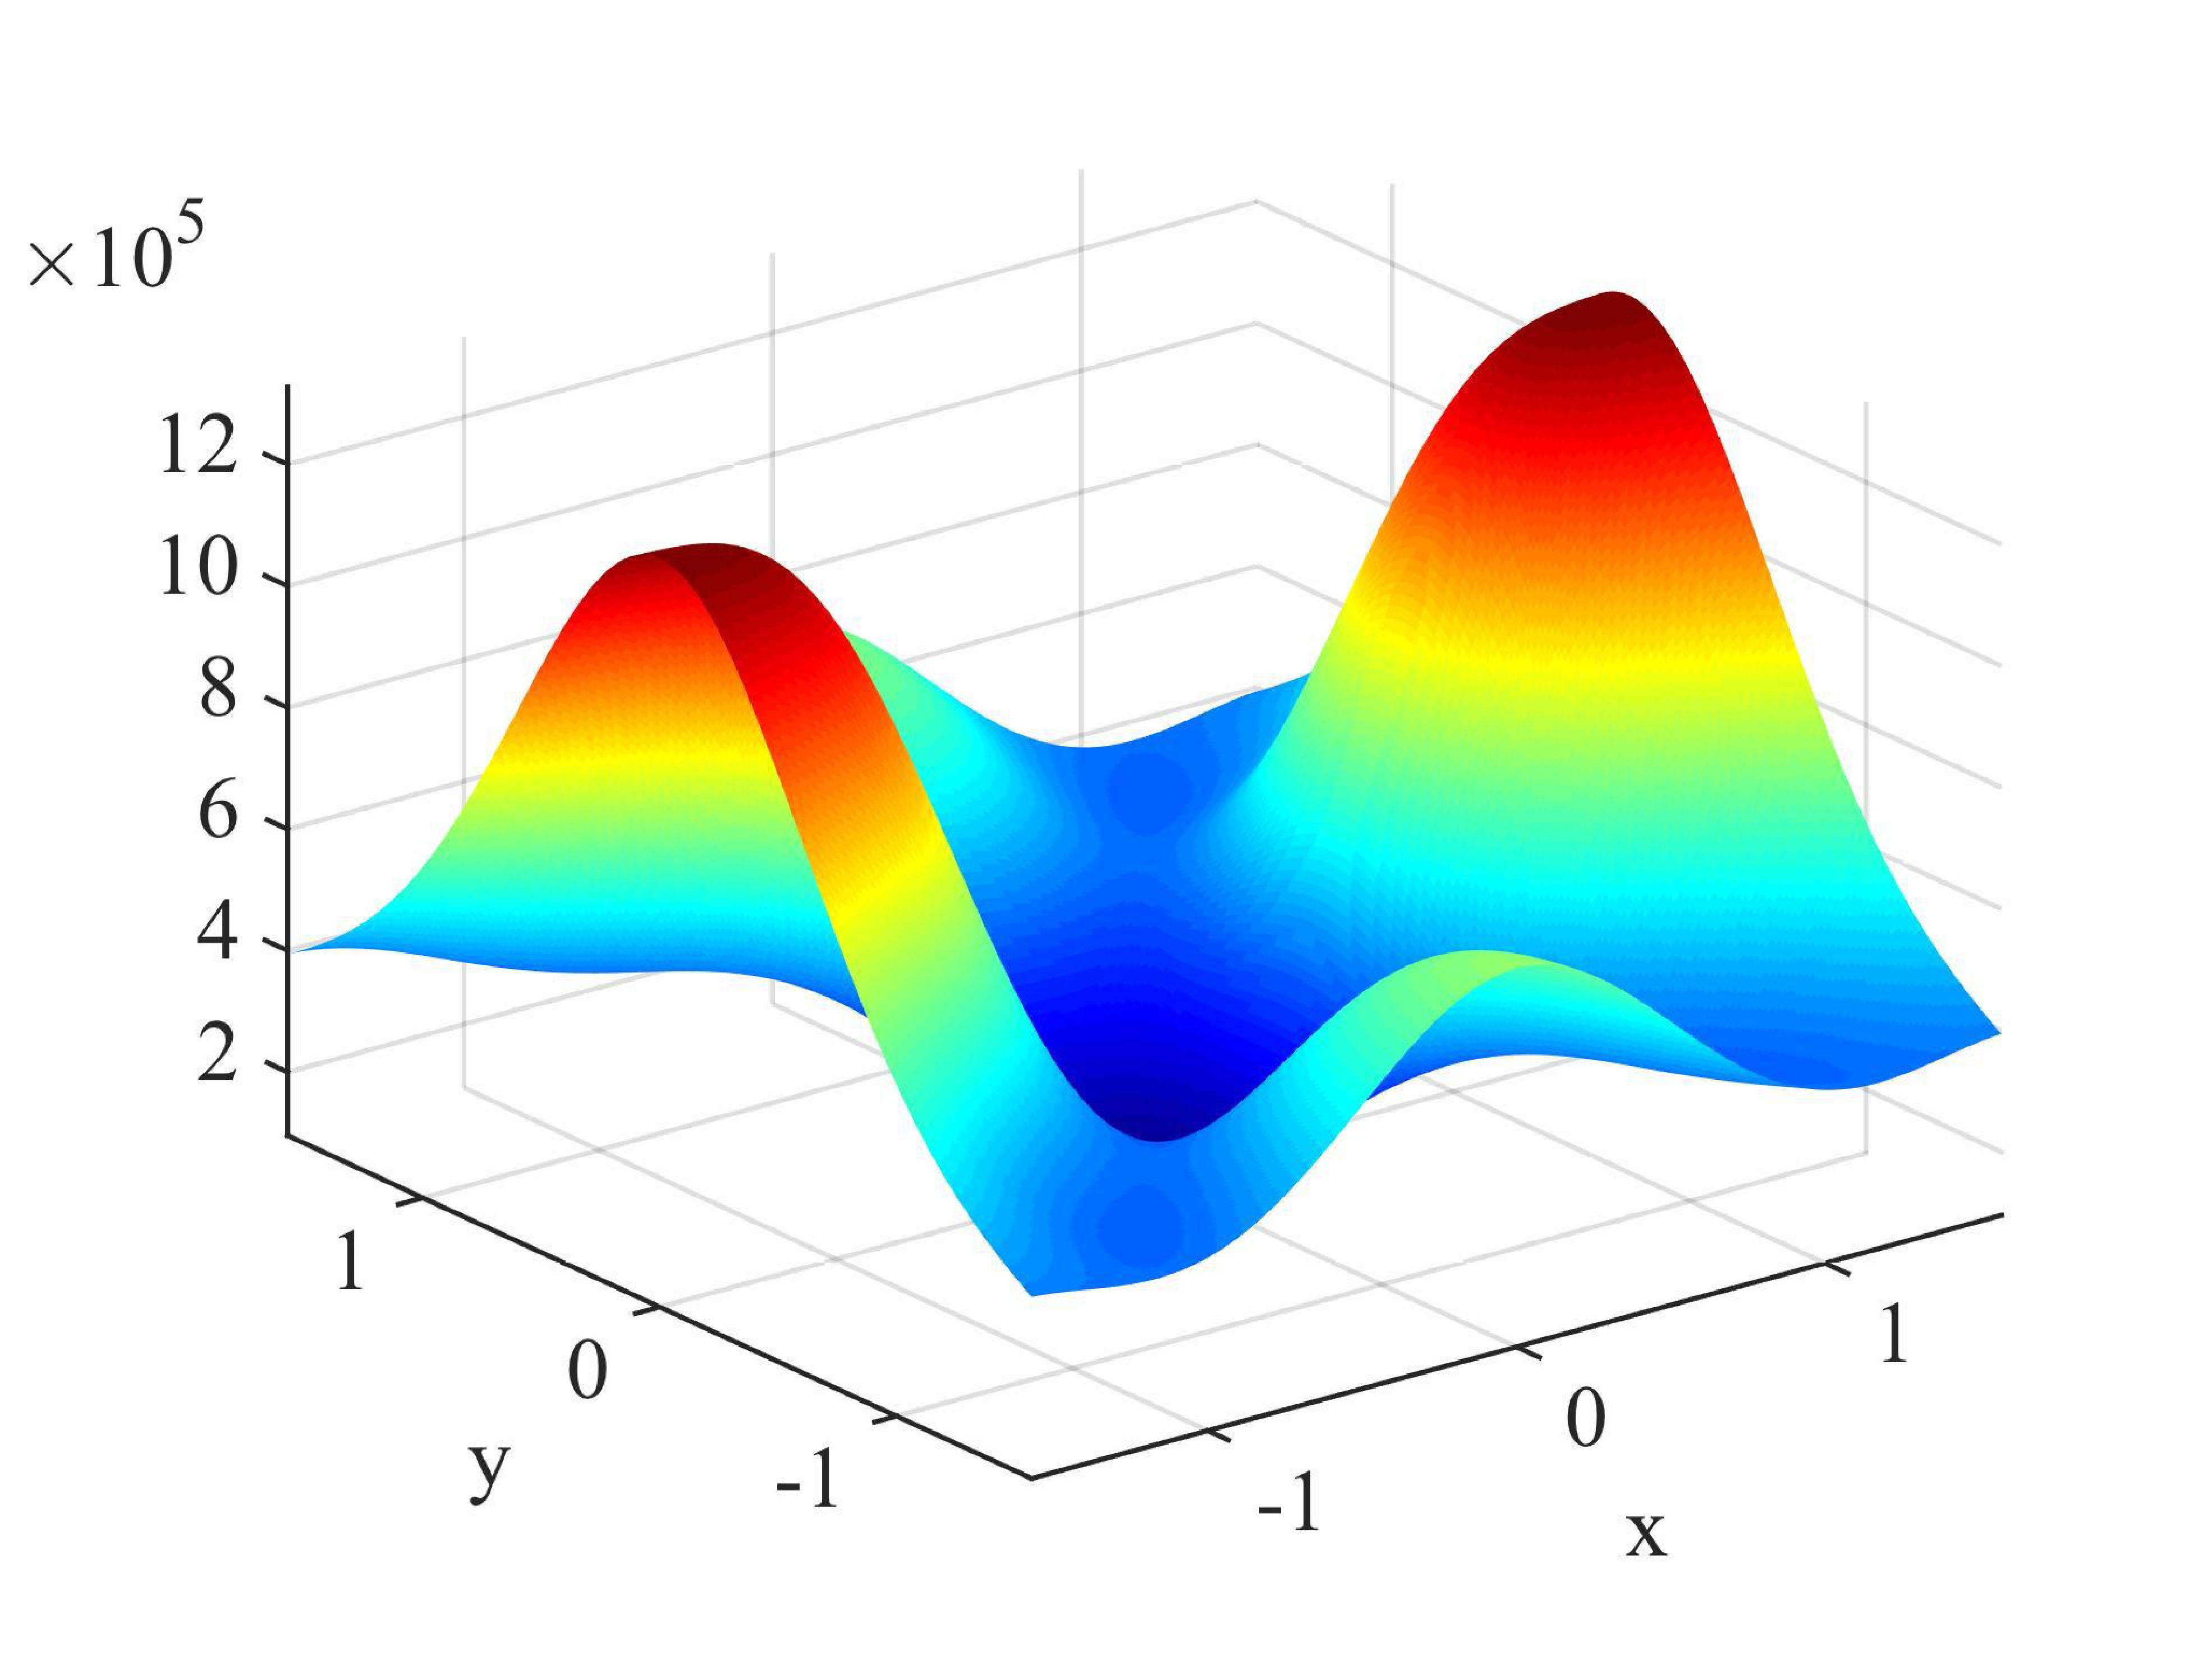
\includegraphics[width=0.45\textwidth]
   {figs/aniso_uniaxial_tangent_detA_F1p0074.pdf}
 } \subfigure[$F_{11}=1.0762$]{
   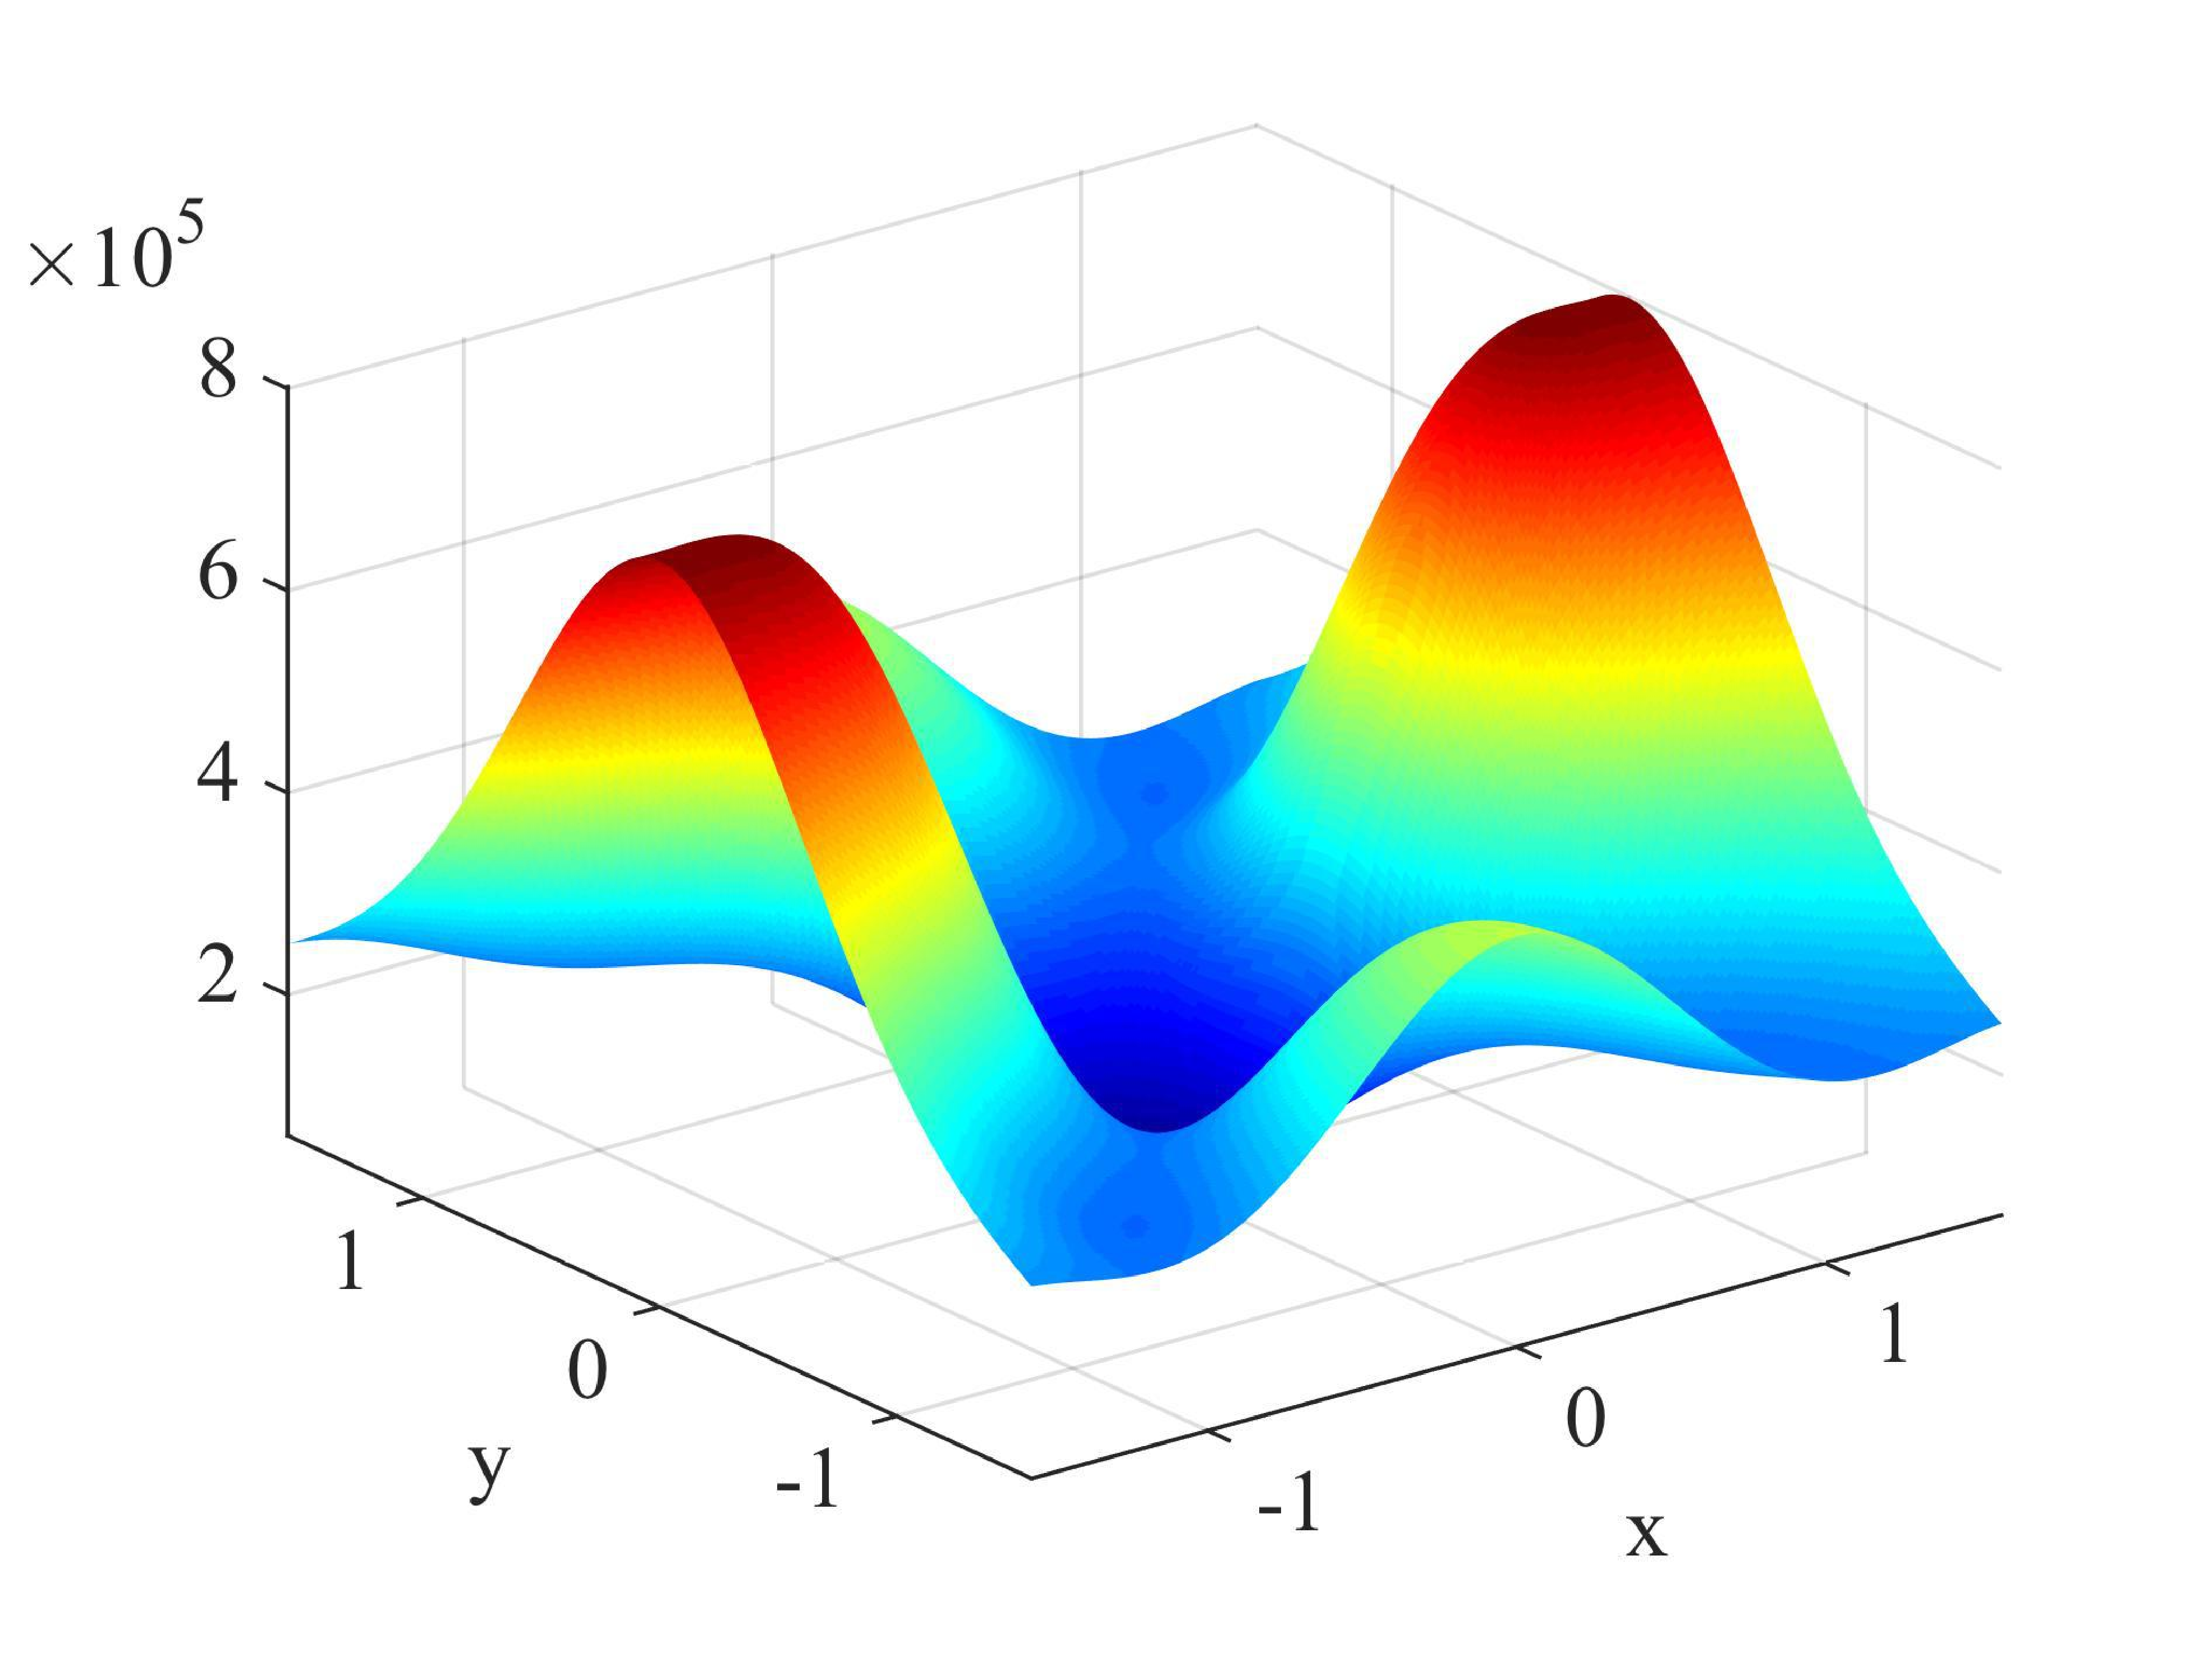
\includegraphics[width=0.45\textwidth]
   {figs/aniso_uniaxial_tangent_detA_F1p0762.pdf}
 } \subfigure[$F_{11}=1.1583$]{
   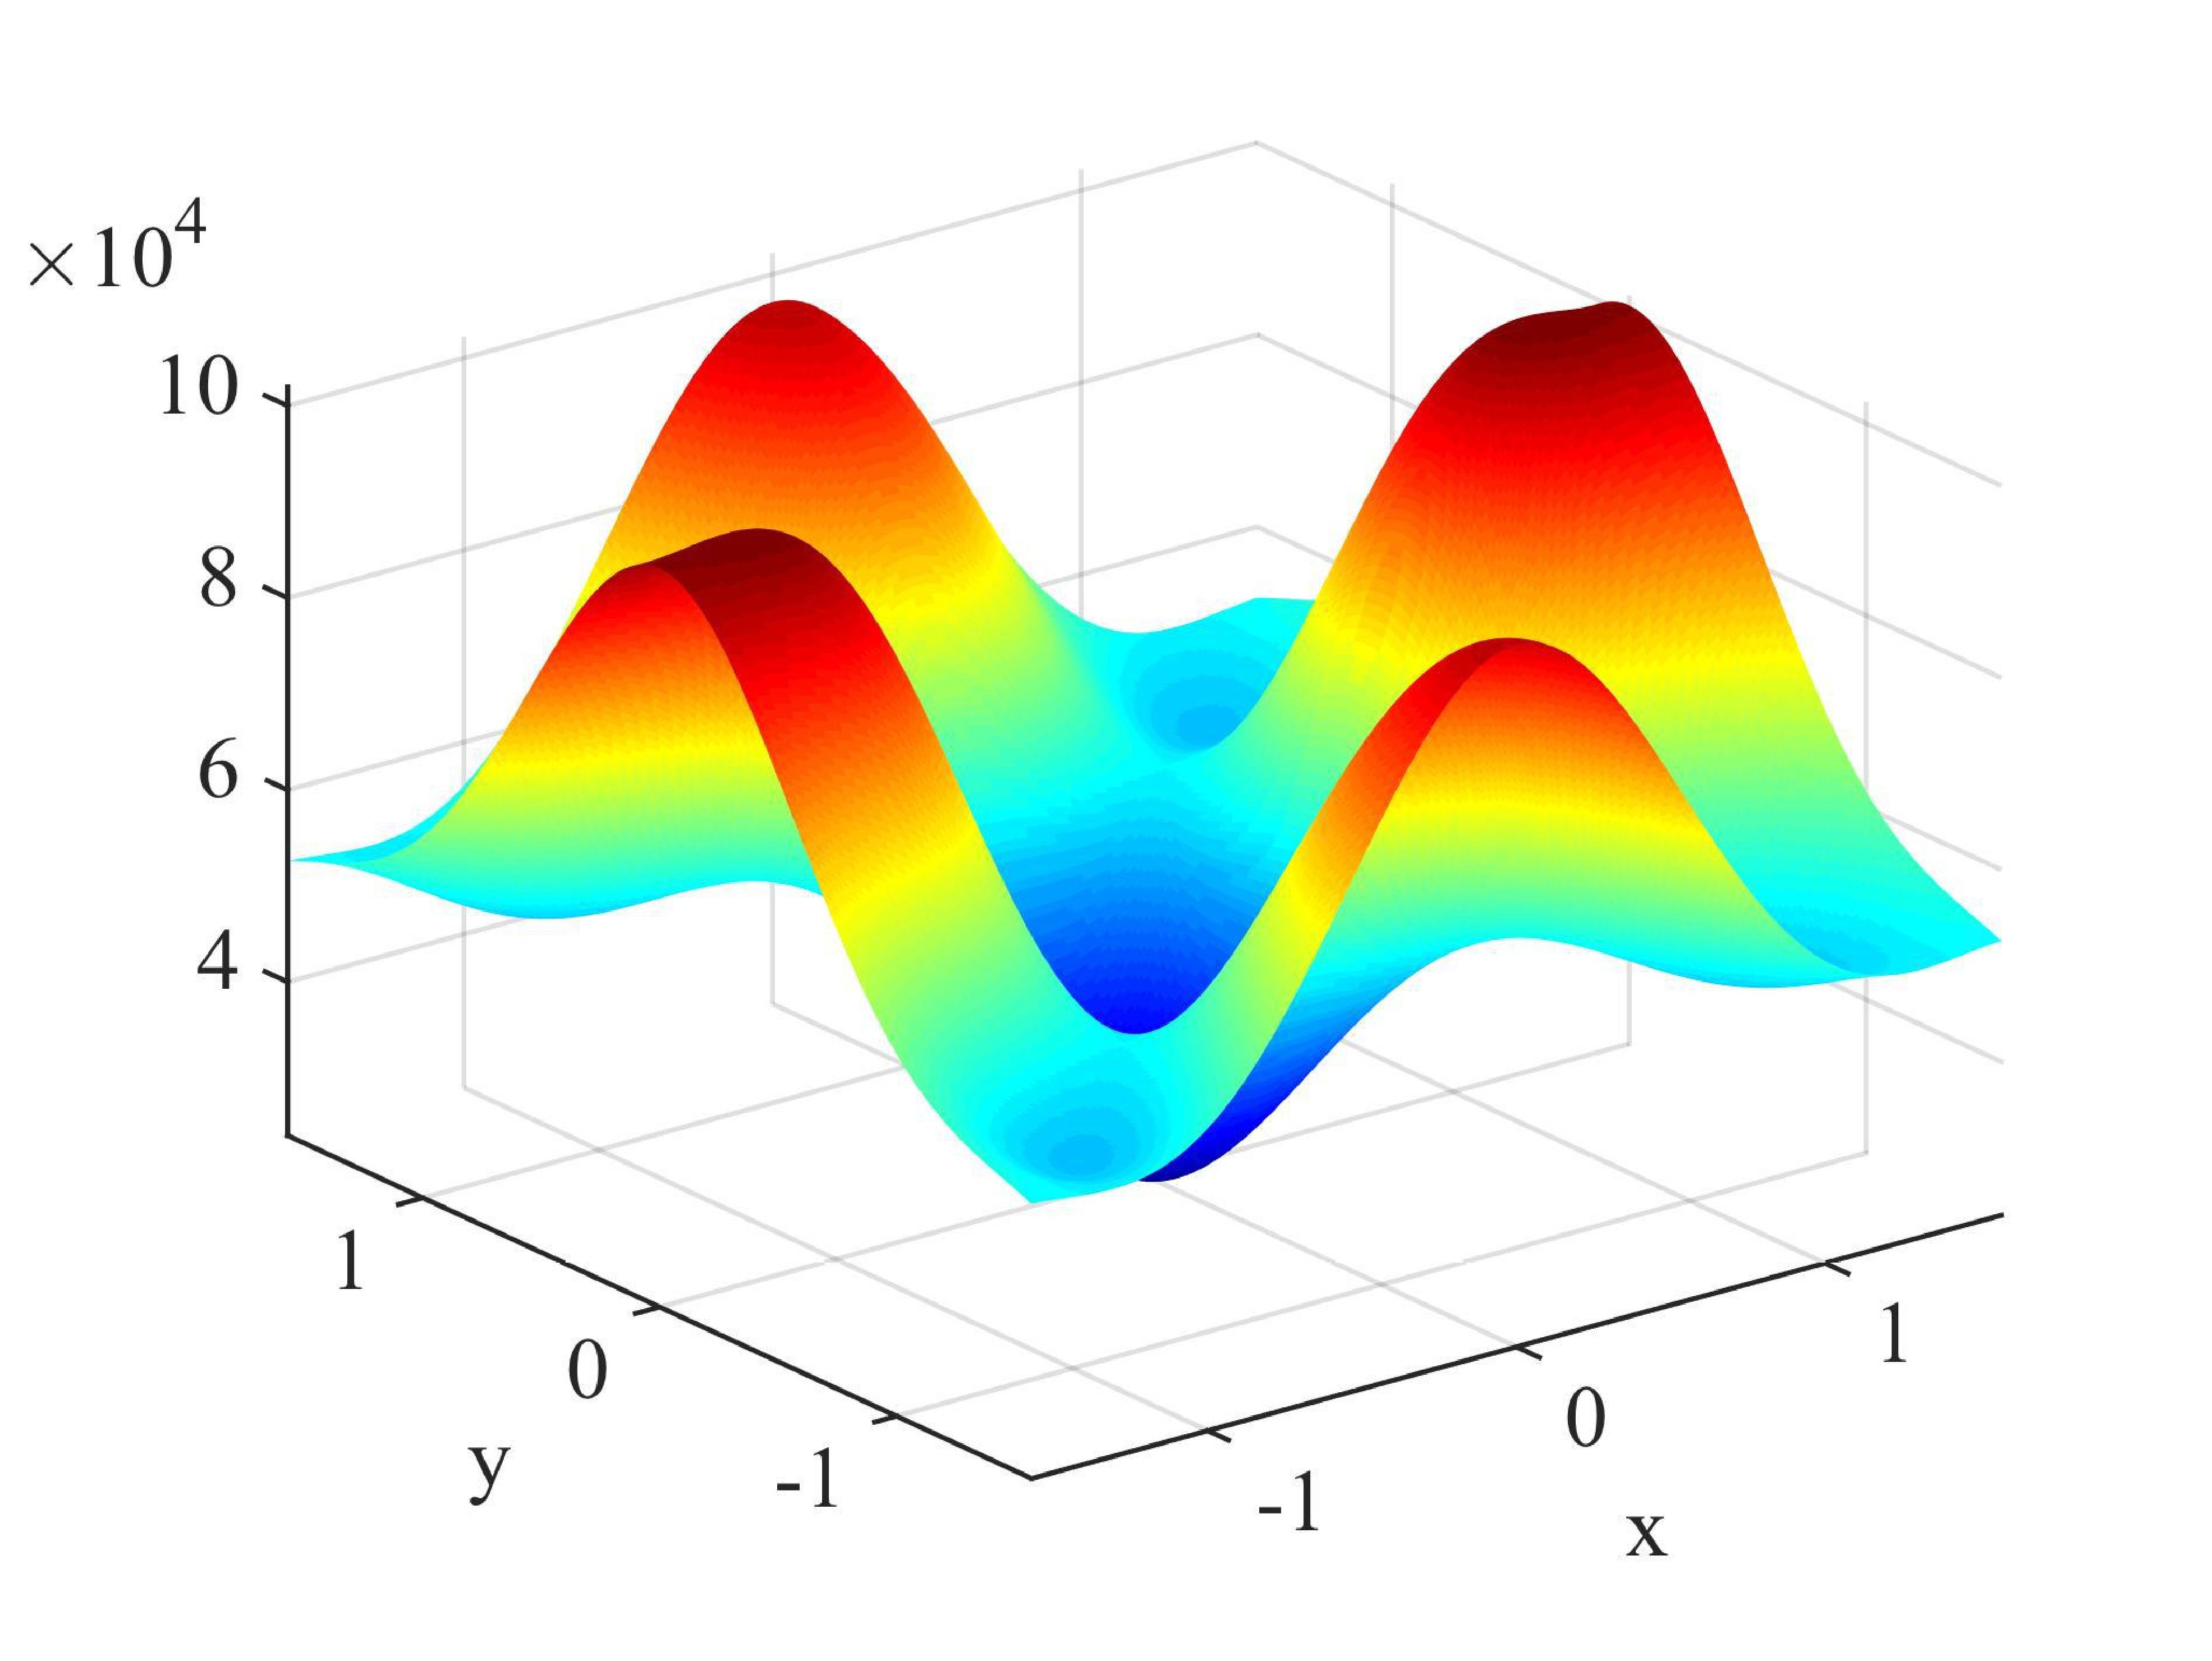
\includegraphics[width=0.45\textwidth]
   {figs/aniso_uniaxial_tangent_detA_F1p1583.pdf}
 } \subfigure[$F_{11}=1.1798$ (bifurcation)]{
   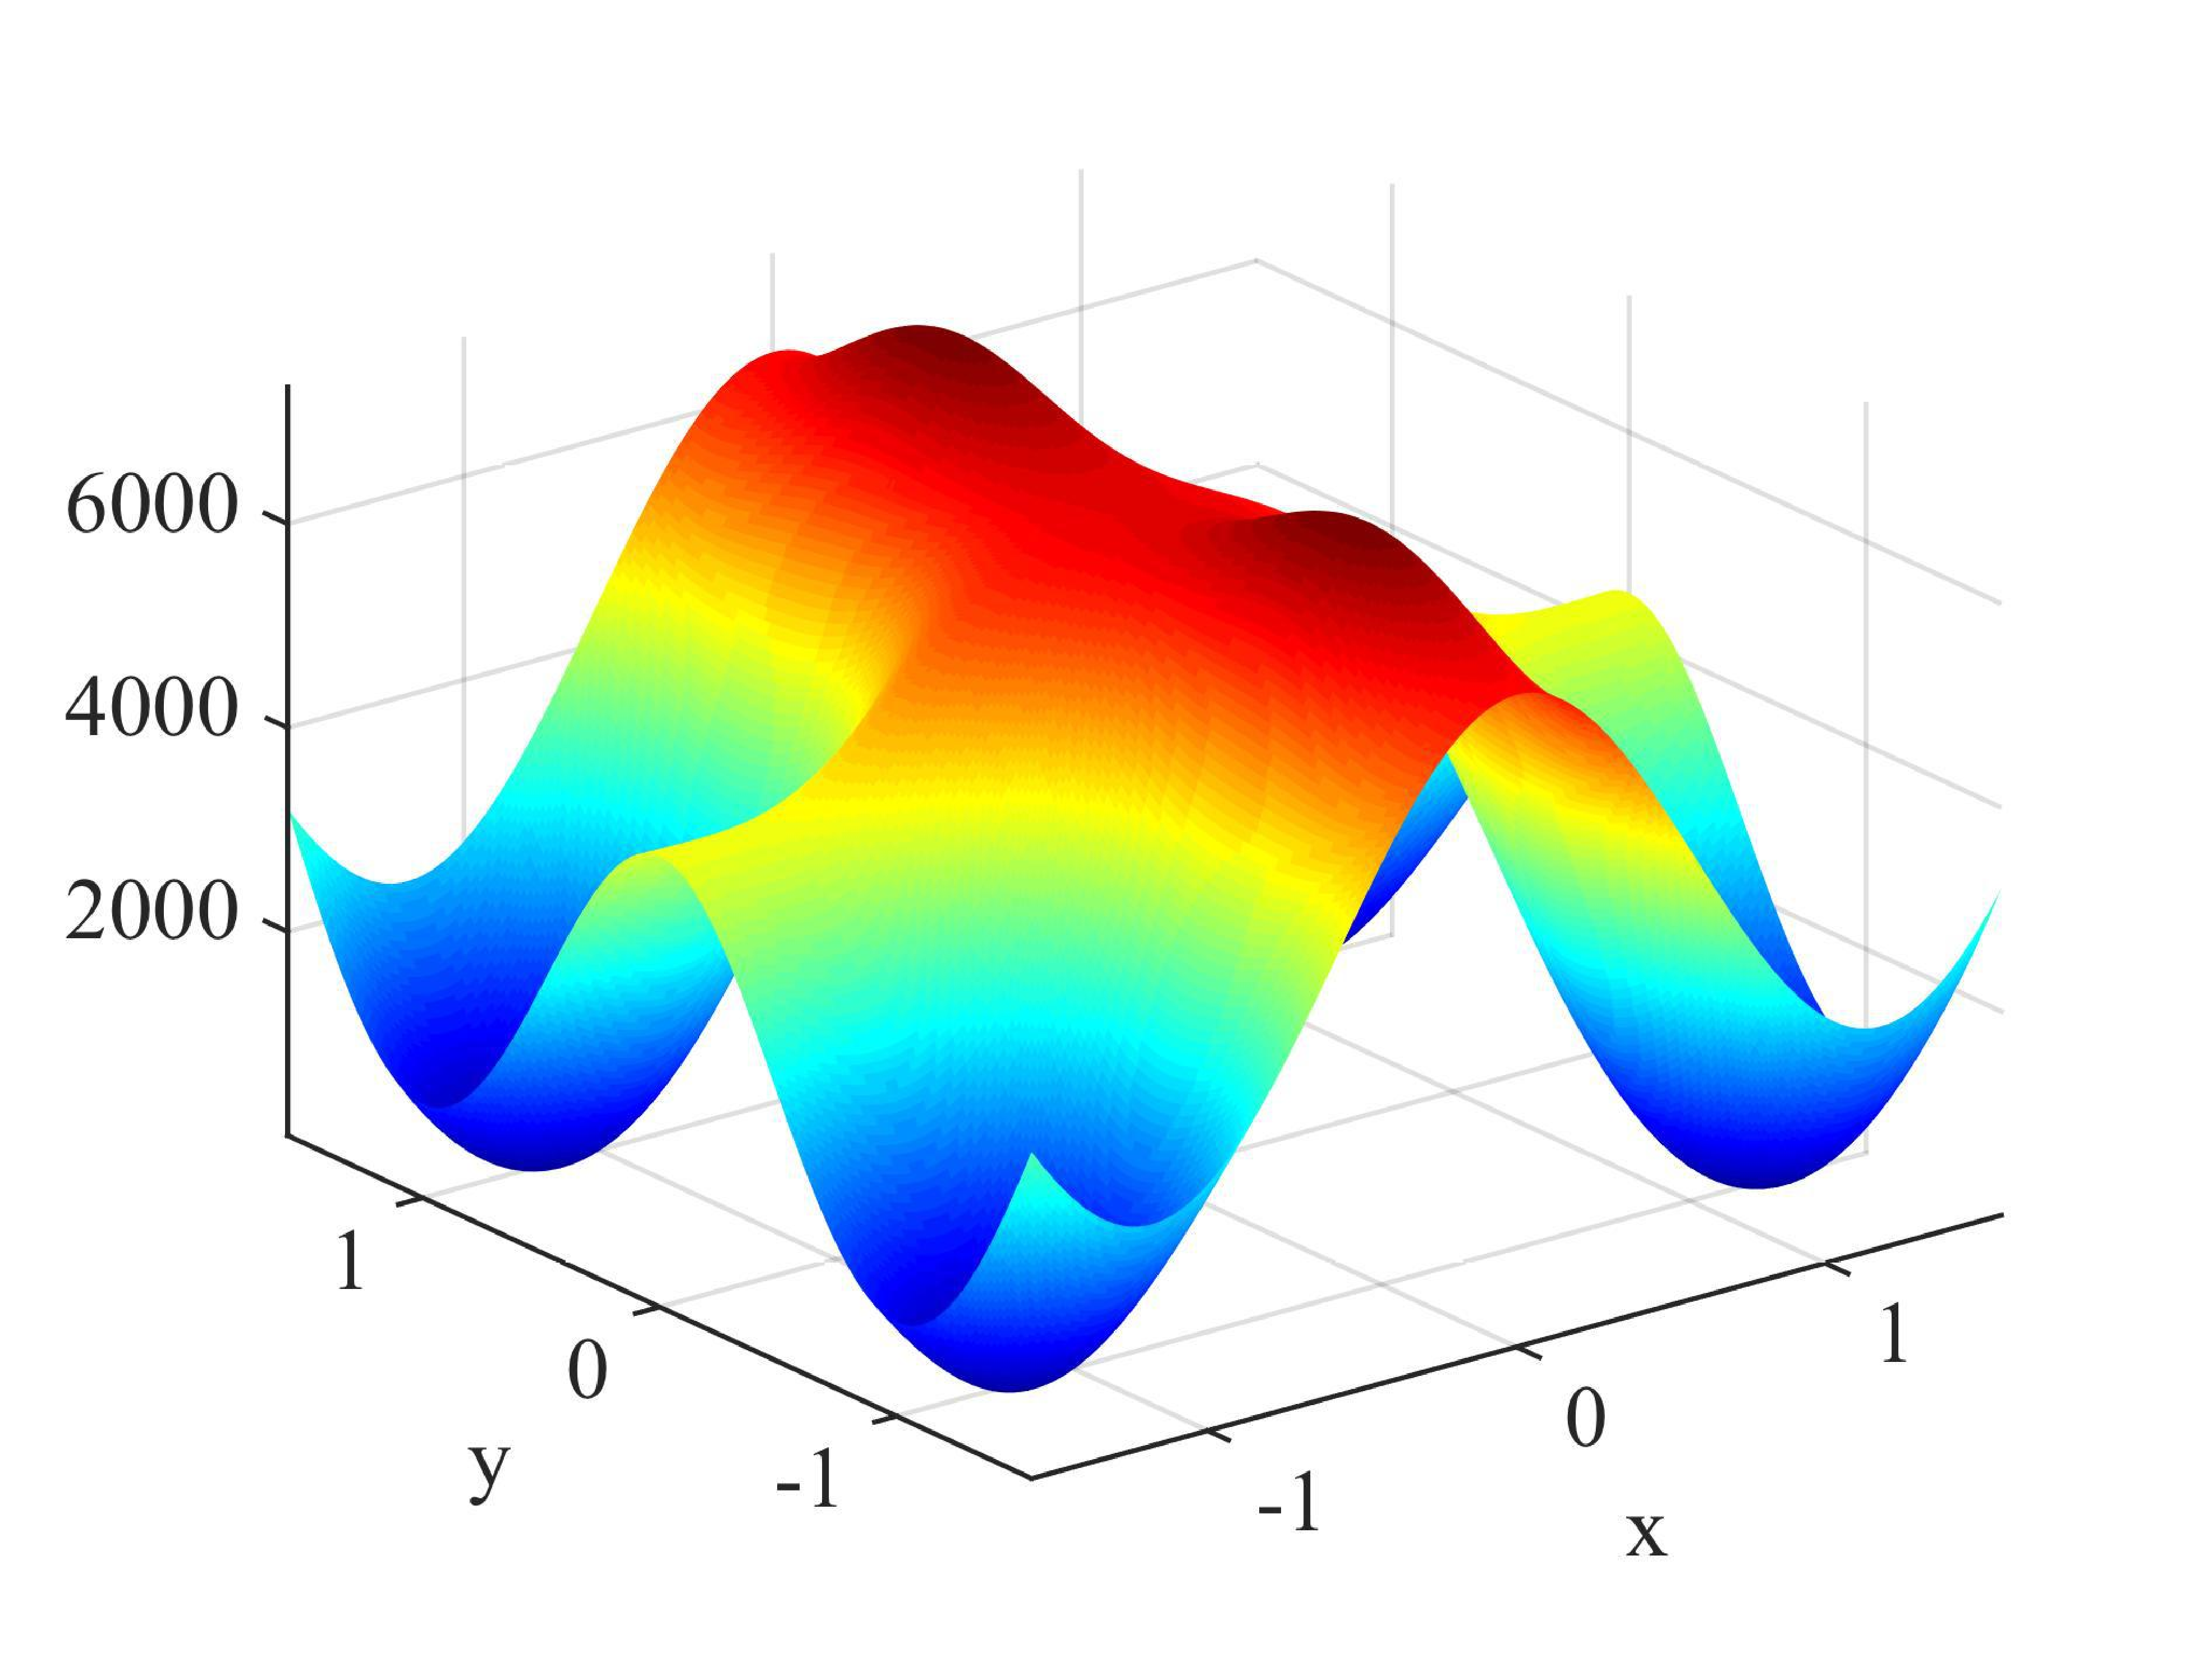
\includegraphics[width=0.45\textwidth]
   {figs/aniso_uniaxial_tangent_detA_F1p1798.pdf}
 }
   \caption{Tangent parametrization: landscapes of det$\bA$ 
   for uniaxial tension test on finite deformation anisotropic model at
   different axial stretch levels.}
   \label{fig:aniso_tangent_detA}
 \end{figure} 

\begin{figure}[H]
   \centering \subfigure[$F_{11}=1.0074$]{
   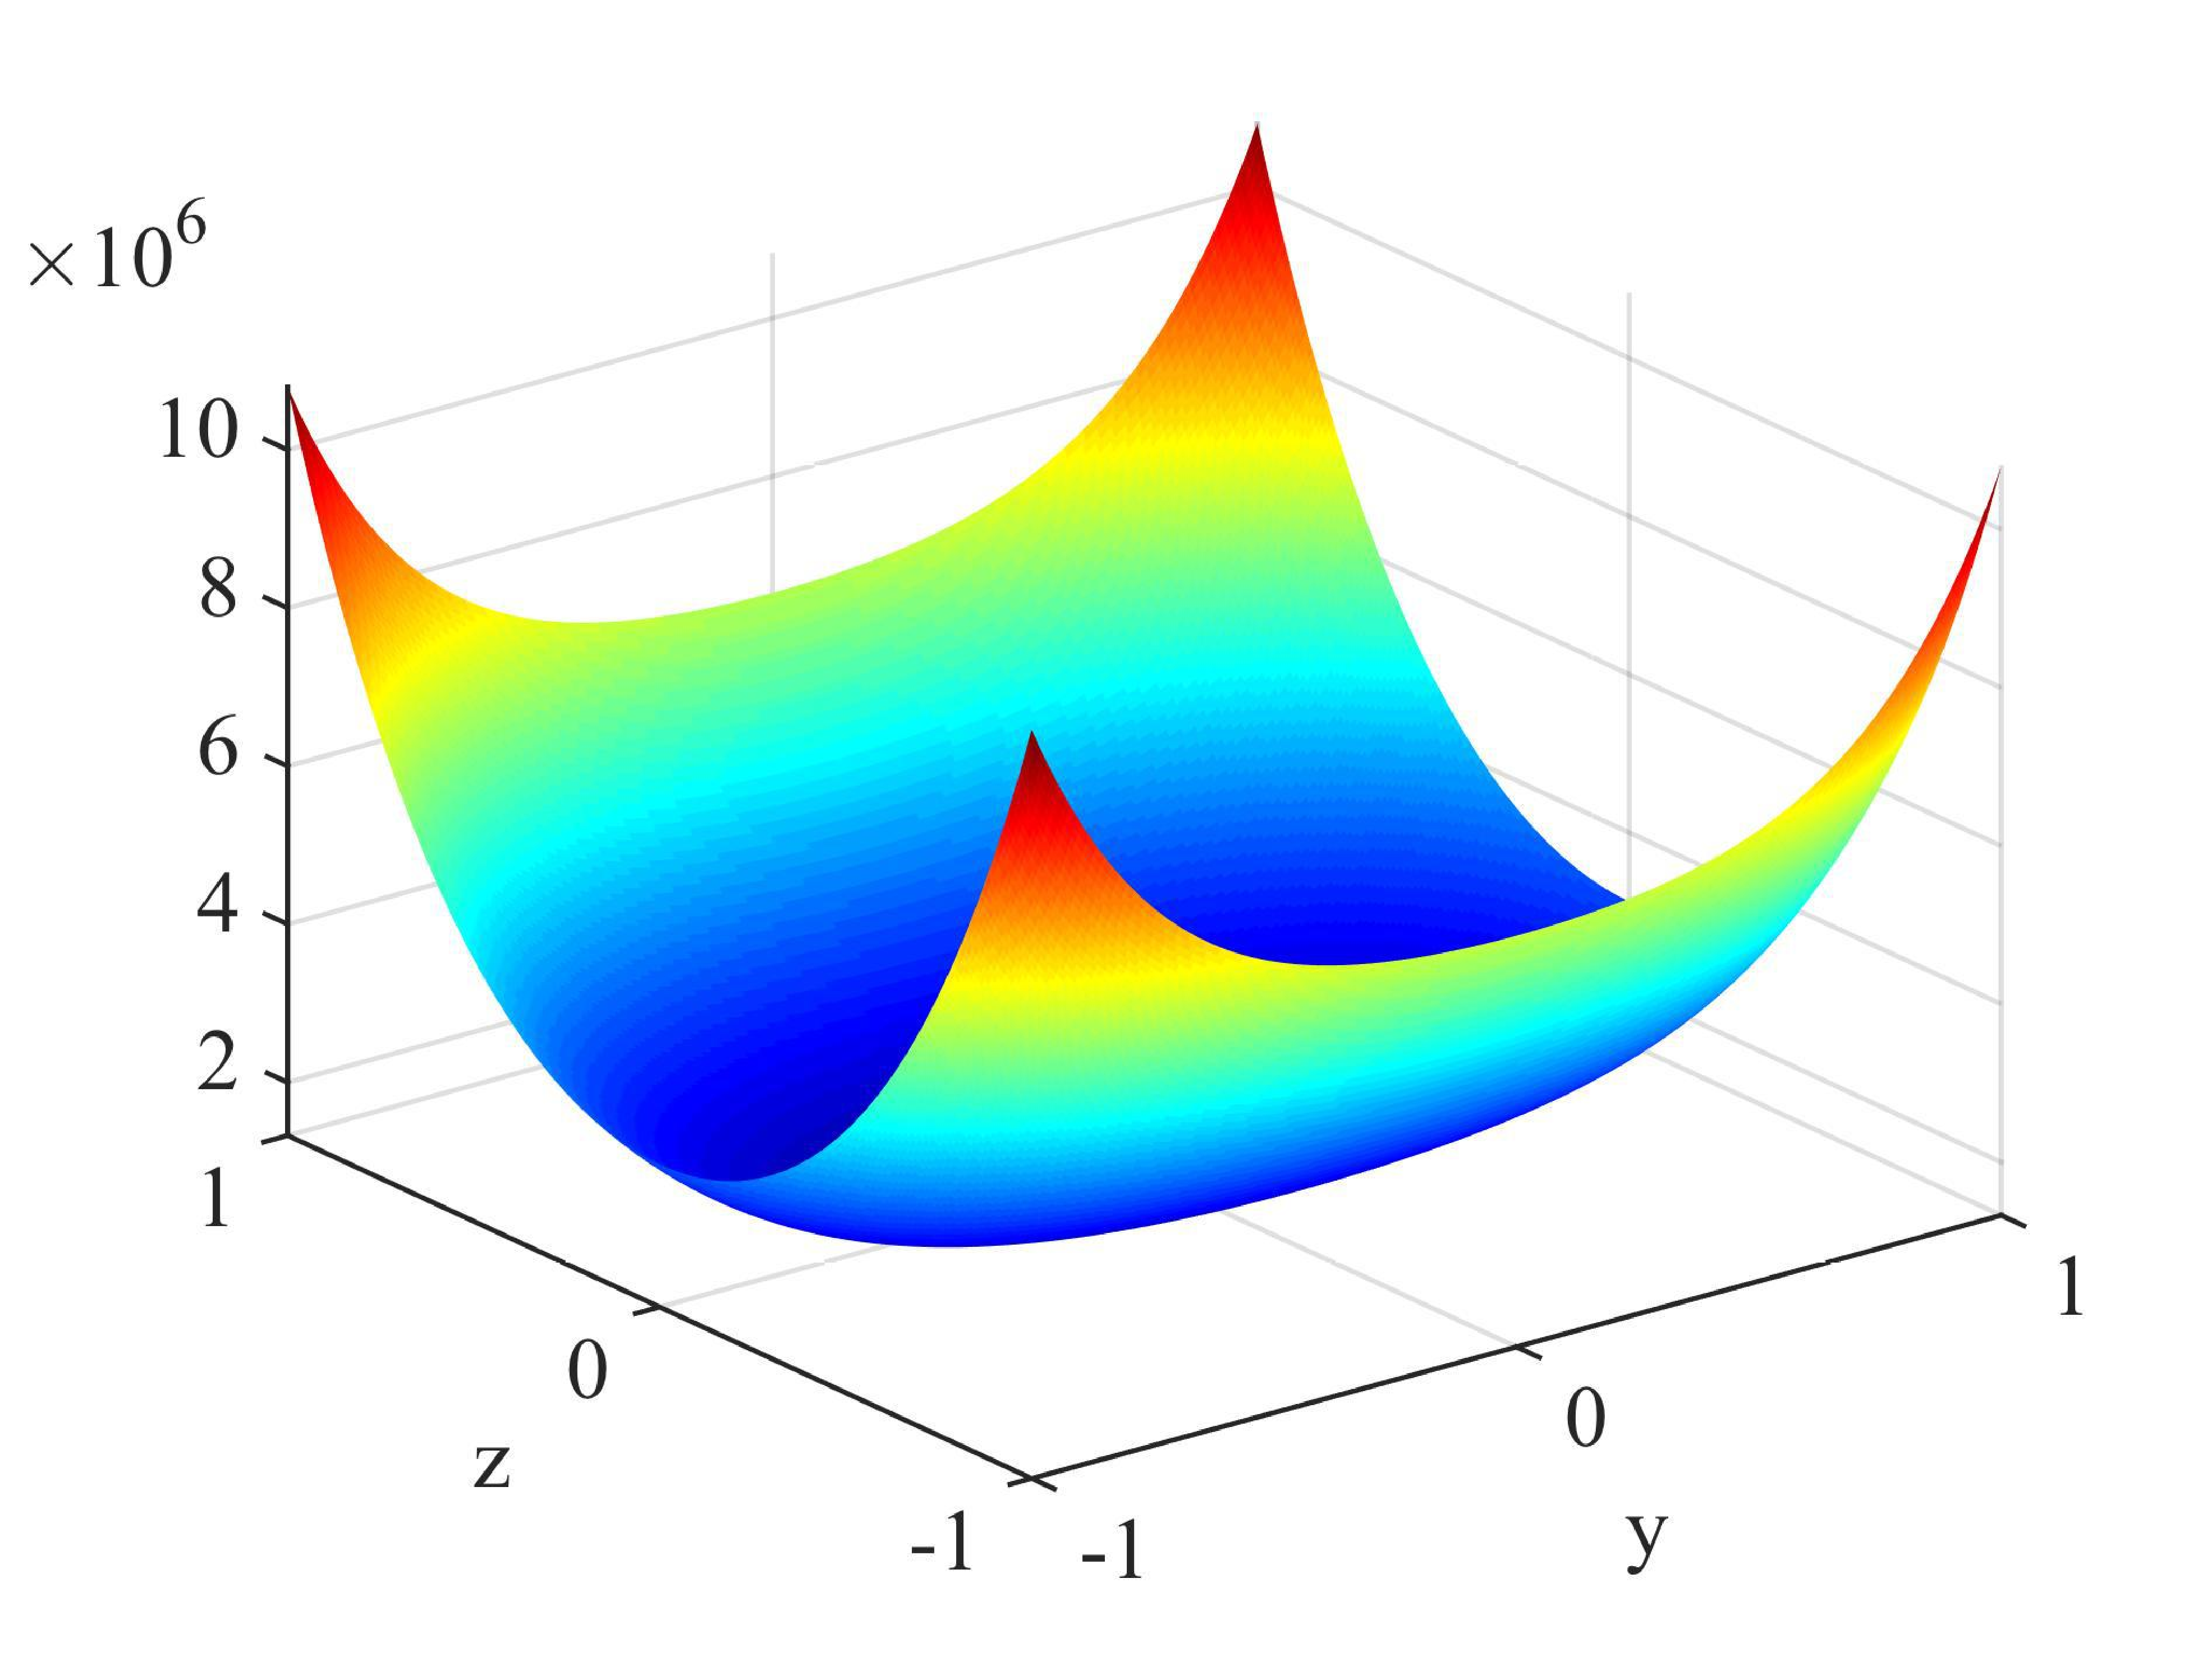
\includegraphics[width=0.45\textwidth]
   {figs/aniso_uniaxial_cartesian_detA_F1p0074.pdf}
 } \subfigure[$F_{11}=1.0762$]{
   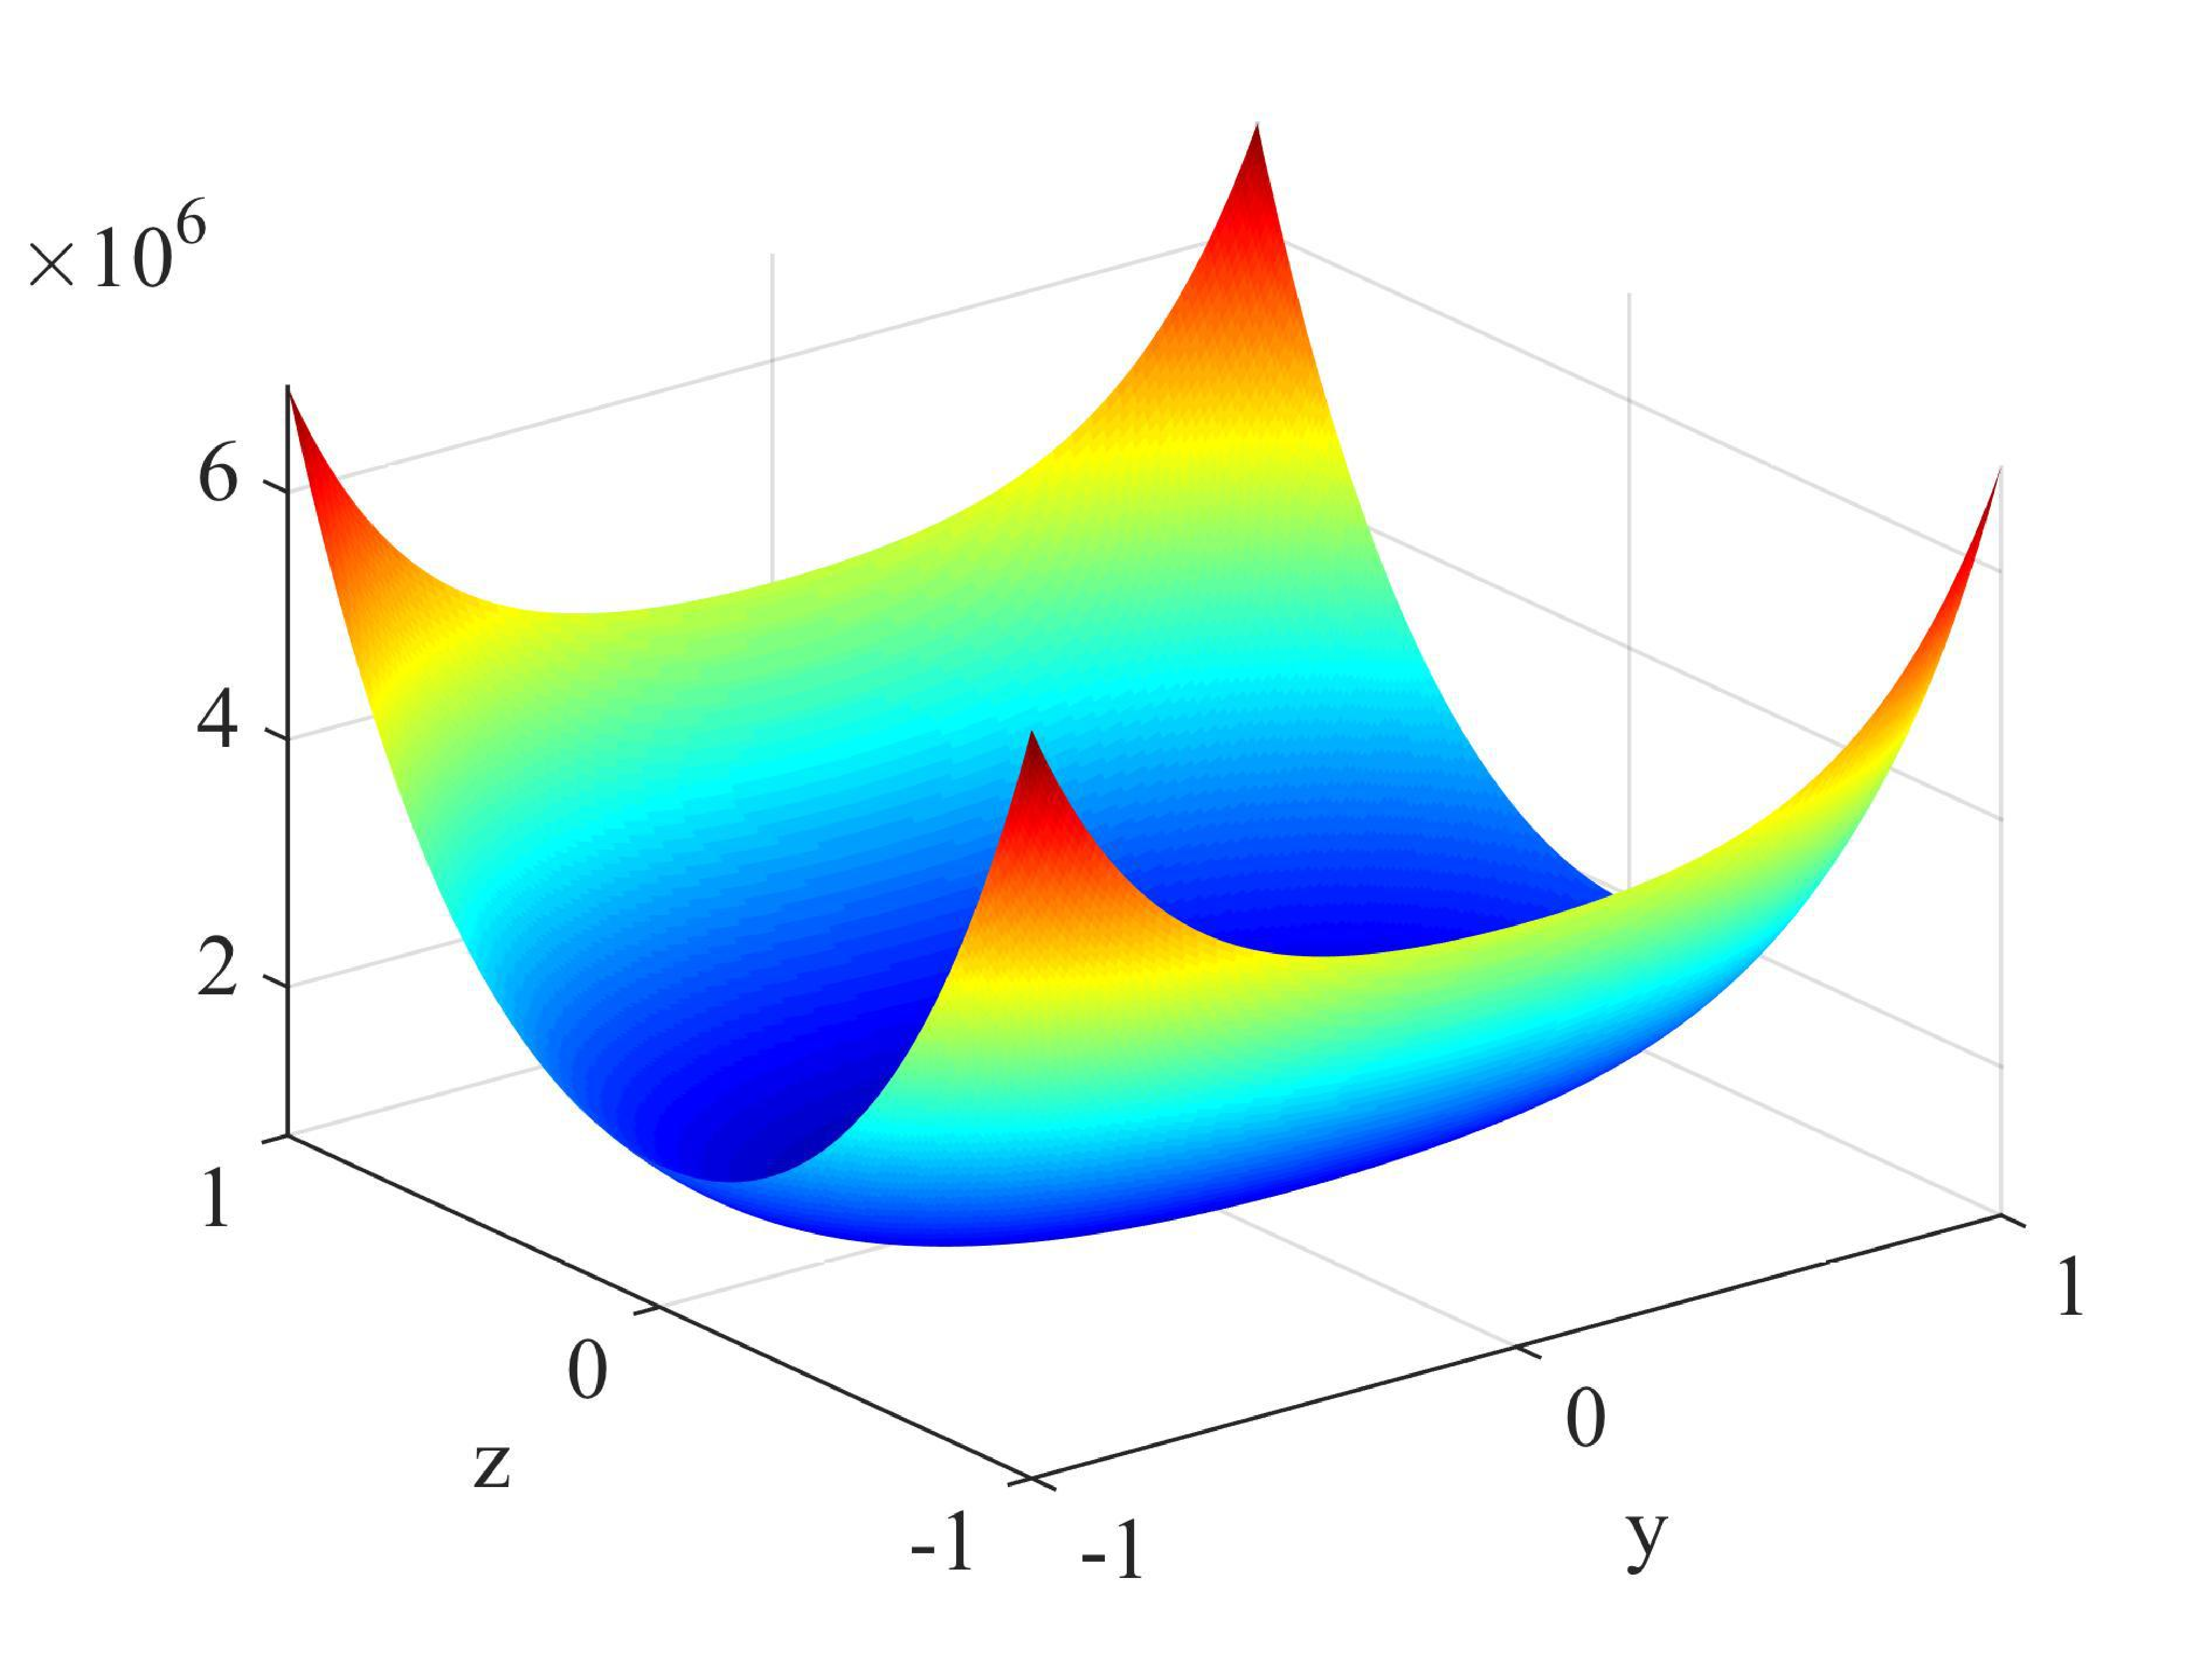
\includegraphics[width=0.45\textwidth]
   {figs/aniso_uniaxial_cartesian_detA_F1p0762.pdf}
 } \subfigure[$F_{11}=1.1583$]{
   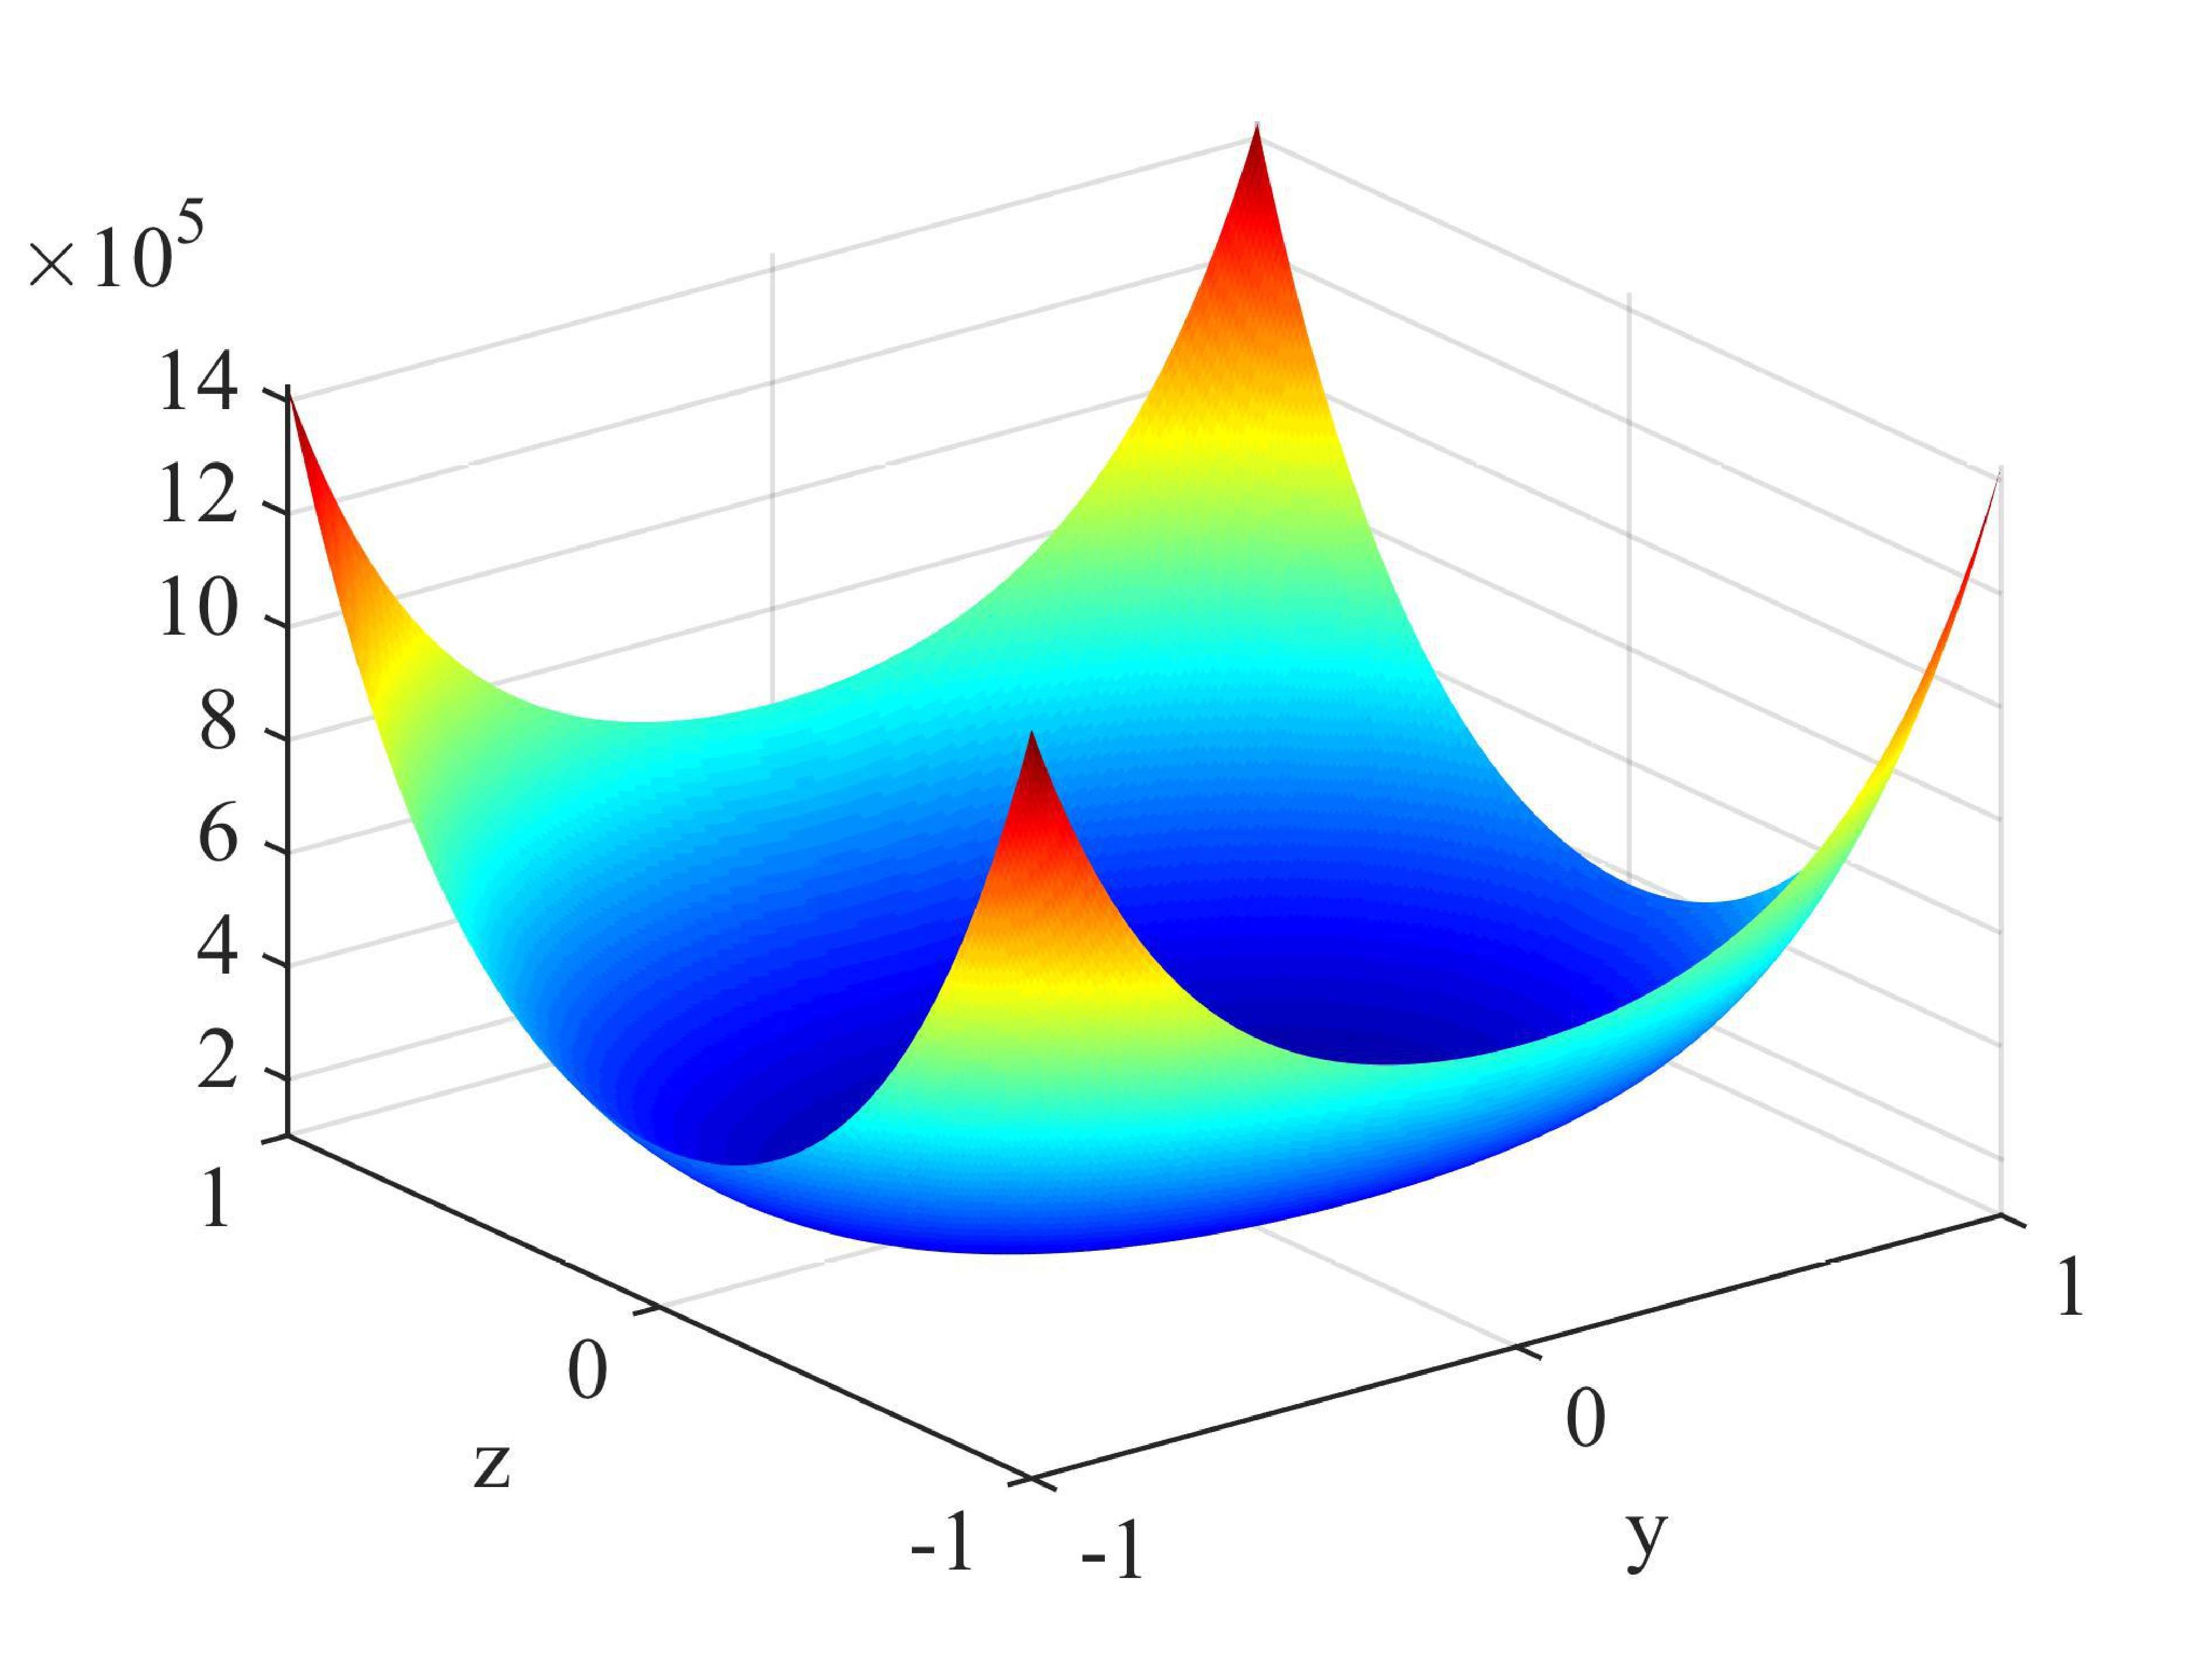
\includegraphics[width=0.45\textwidth]
   {figs/aniso_uniaxial_cartesian_detA_F1p1583.pdf}
 } \subfigure[$F_{11}=1.1798$ (bifurcation)]{
   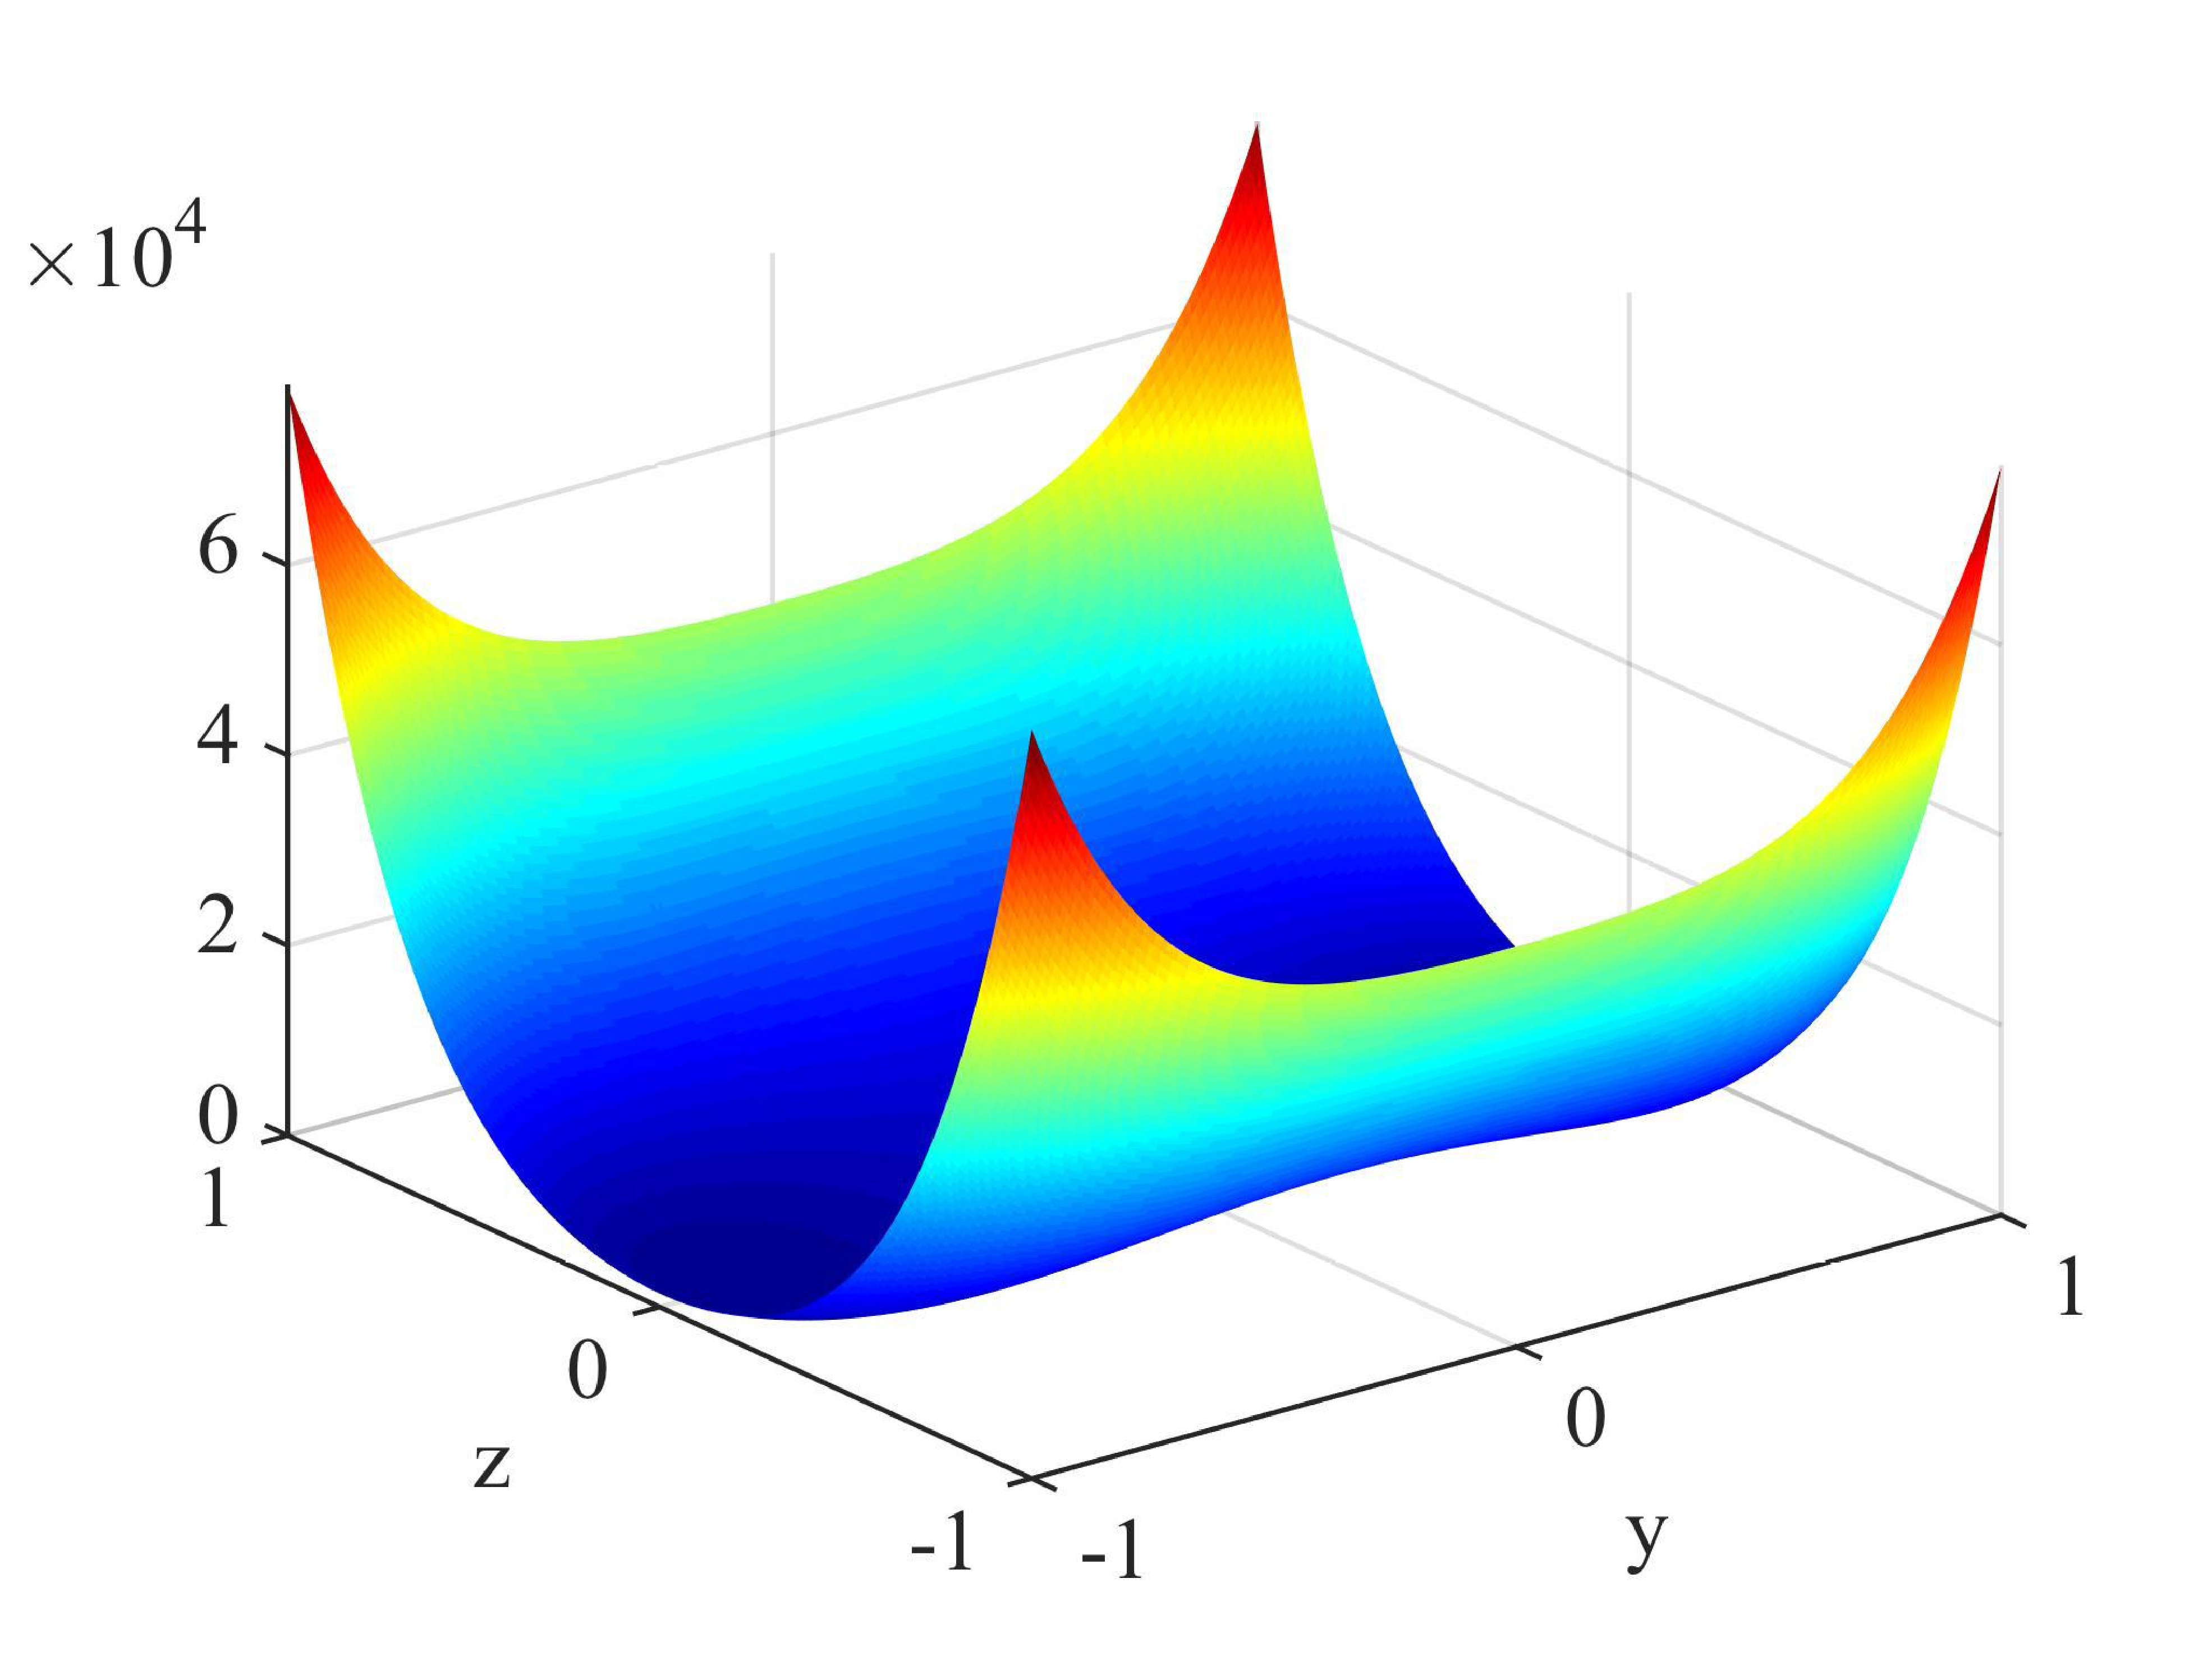
\includegraphics[width=0.45\textwidth]
   {figs/aniso_uniaxial_cartesian_detA_F1p1798.pdf}
 }
   \caption{Cartesian parametrization: landscapes of det$\bA$ 
   for uniaxial tension test on finite deformation anisotropic model at
   different axial stretch levels.}
   \label{fig:aniso_cartesian_detA}
 \end{figure} 

As can be seen from Figure~\ref{fig:aniso_cartesian_detA}, the 
Cartesian parametrization again results in a simple `bowl-shaped' 
landscape of the determinant function consistently throughout the 
loading process, which is in contrast to other more complex landscapes 
using alternative parametrizations shown in Figures~ 
\ref{fig:aniso_spherical_detA} for spherical, 
\ref{fig:aniso_stereographic_detA} for stereographic and 
\ref{fig:aniso_tangent_detA} for tangent parametrizations. 

As in the case of the small deformation model example in 
Section \ref{subsec:isotropic}, the robustness of different 
parametrizations on the detection of material bifurcation is analyzed 
by randomly generating a single initial point for the Newton iterative 
solve, i.e., no sweep algorithm is used. A total of 1000 sets of 
random initial guess is generated for each parametrization. The 
success rate and computational cost are recorded and summarized in 
Table~\ref{tab:aniso_axial_random_para}. The results are consistent 
with the small deformation model example, i.e., the Cartesian 
parametrization is most robust and at the same time, computationally efficient. 

\begin{table}[H]
  \begin{center}
    %\begin{tabular}{ lp{1.5cm} lp{1.5cm} lp{1.5cm} lp{1.5cm} lp{1.5cm} lp{1.5cm}}
    %  \begin{tabular*}{1.0\textwidth}{l | c c c c c}
    \begin{tabular}{l | c c c c c}
      \toprule
        &  Spherical    &   Stereographic   & Projective   &   Tangent   &   Cartesian                 \\
      \midrule
      Success rate ($\%$)                      &    19.4    &    32.3     &    71.5     &    32.3     &     74.4          \\ 
      Averaged iteration count               &    4.43    &    4.91    &    8.04     &    4.57    &    6.93         \\
      Averaged run time (${\mu}s$)     &    256     &    274     &    483      &    245      &    267         \\
      \bottomrule
    \end{tabular}
    \caption{Anisotropic finite deformation model: success rate and computational cost of Newton iterative solve with a single random initial point. A total of 1000 random trials are performed for each parametrization.}
    \label{tab:aniso_axial_random_para}
  \end{center}
\end{table}

Visualizations of the robustness study with 1000 trial runs are shown 
in Figure~\ref{fig:aniso_uniaxial_robust}. If the initial guess leads 
to a success detection of bifurcation and its directions, the point 
will be marked as a solid circle ($\bullet$). Otherwise, it will be 
marked as a cross ($\times$).

\begin{figure}[H]
   \centering \subfigure[Spherical]{
   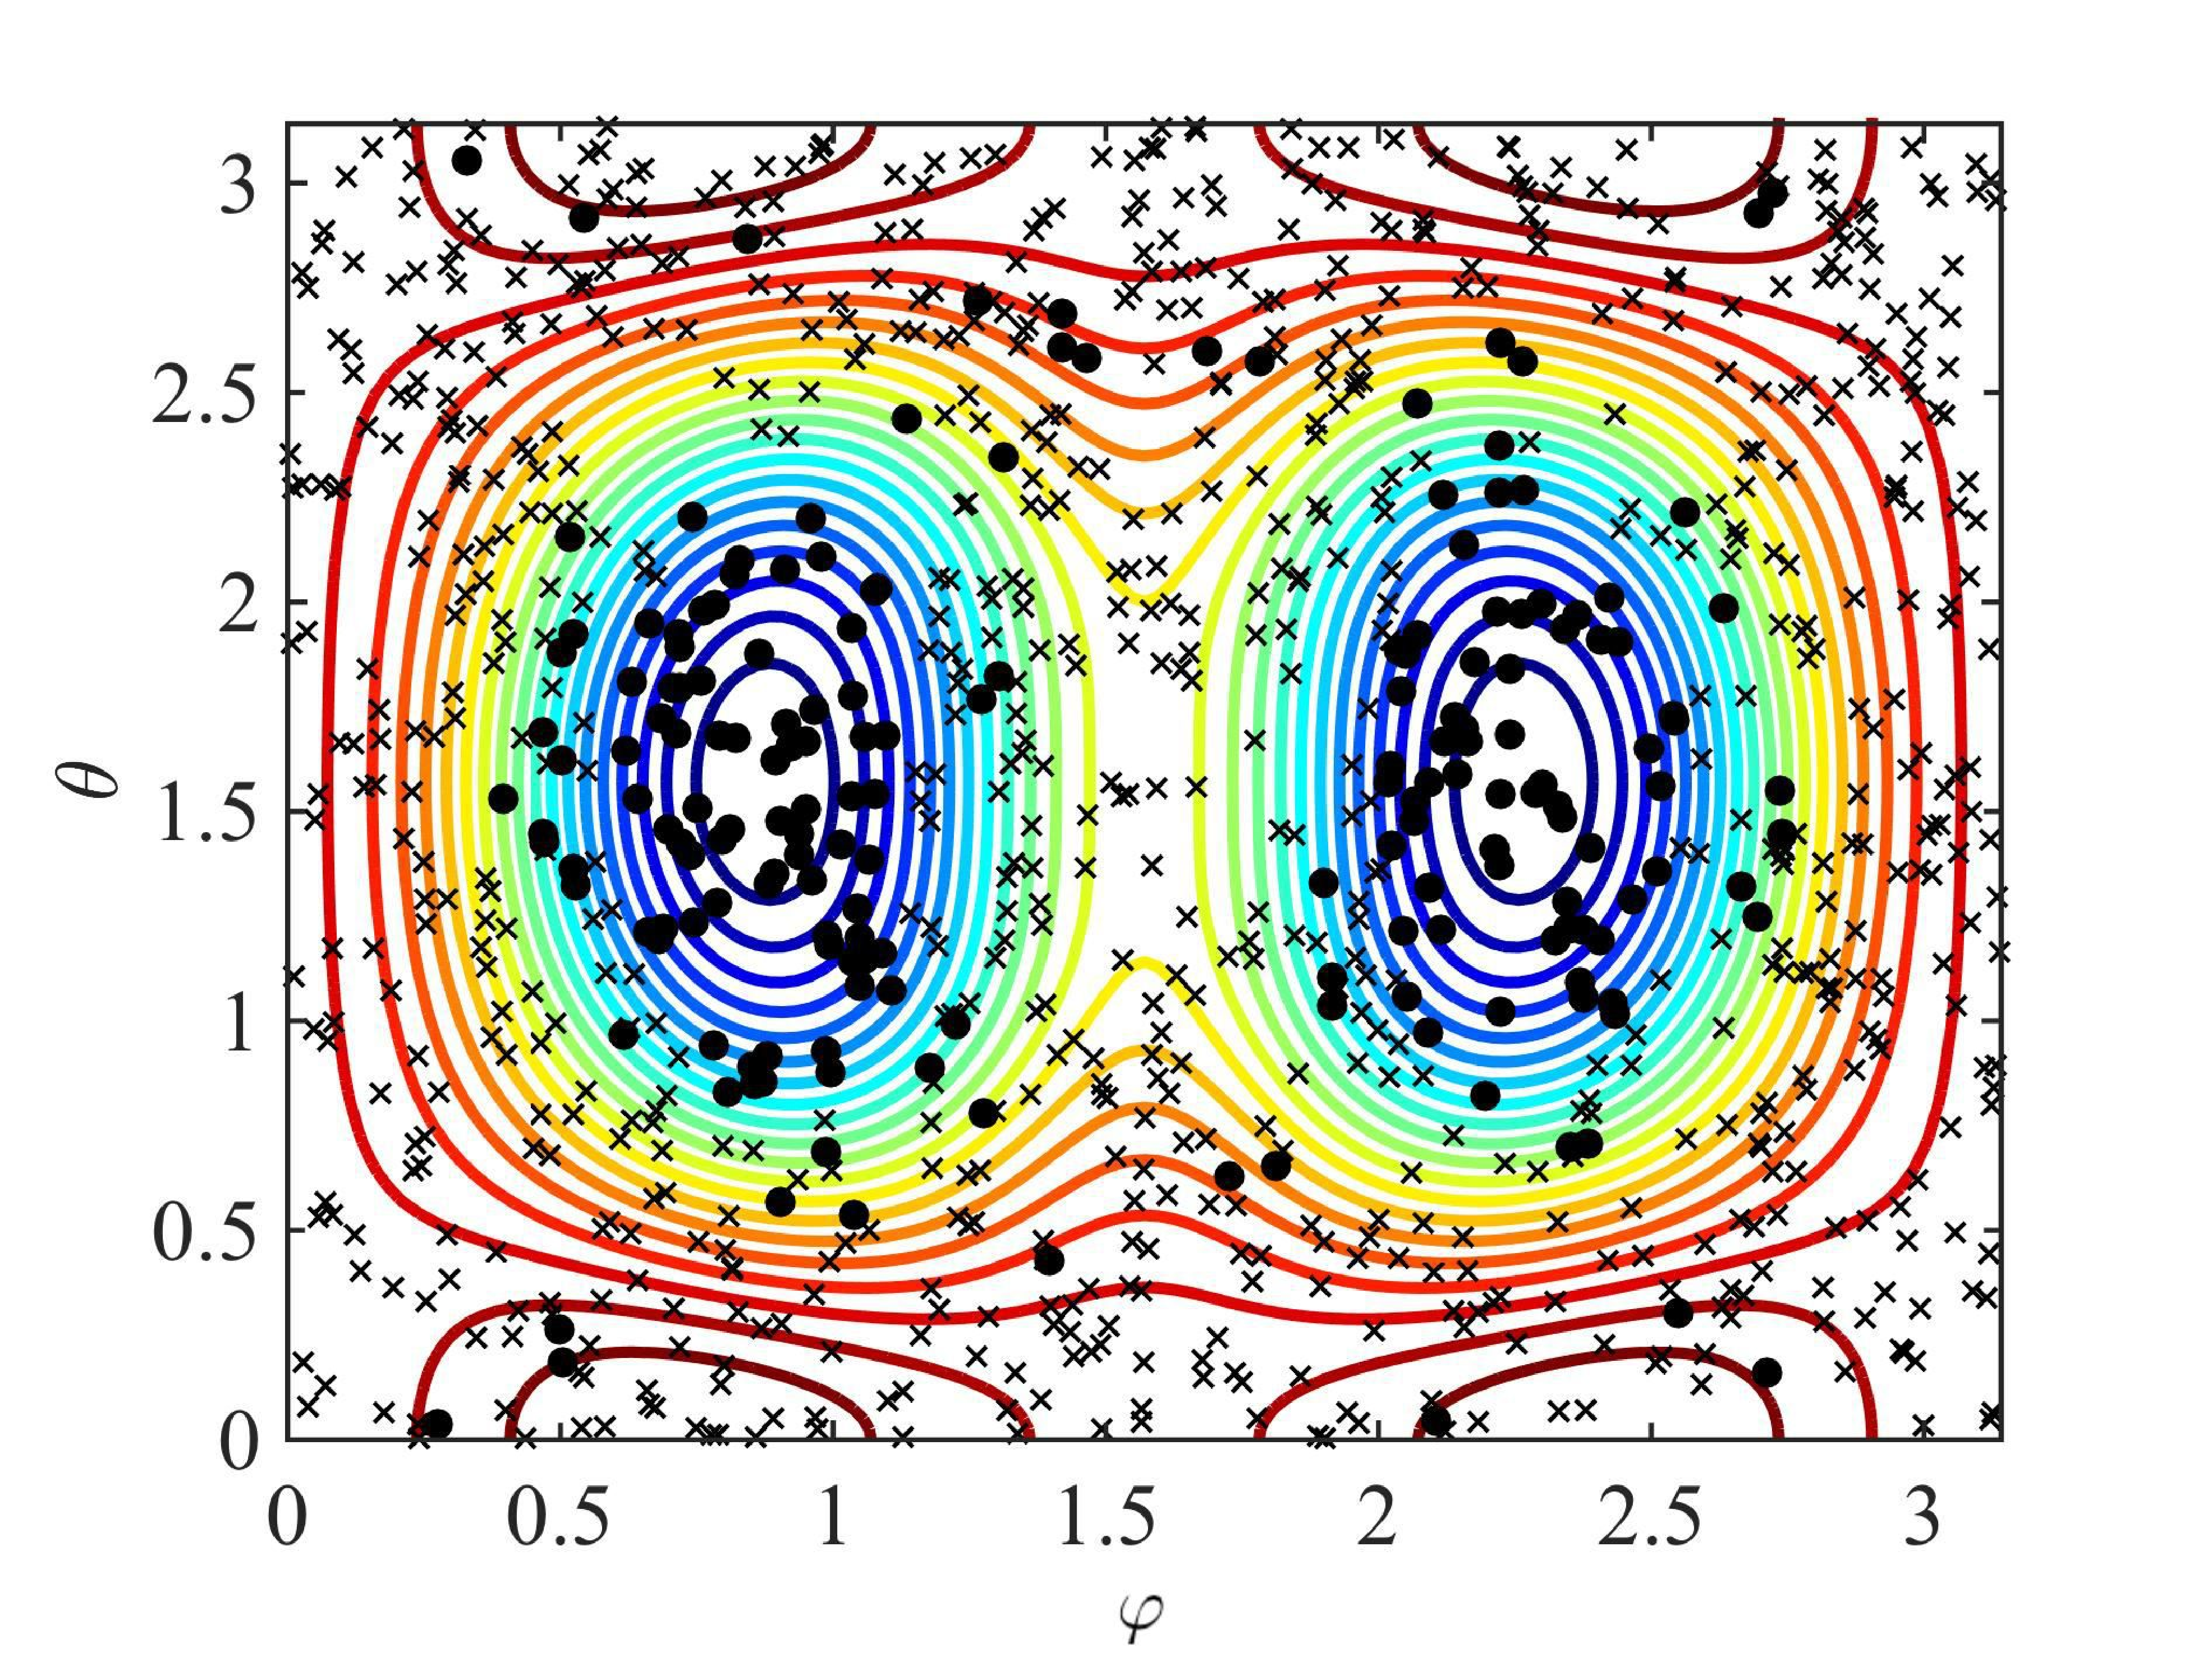
\includegraphics[width=0.45\textwidth]
   {figs/aniso_uniaxial_spherical_random.pdf}
 } \subfigure[Cartesian]{
   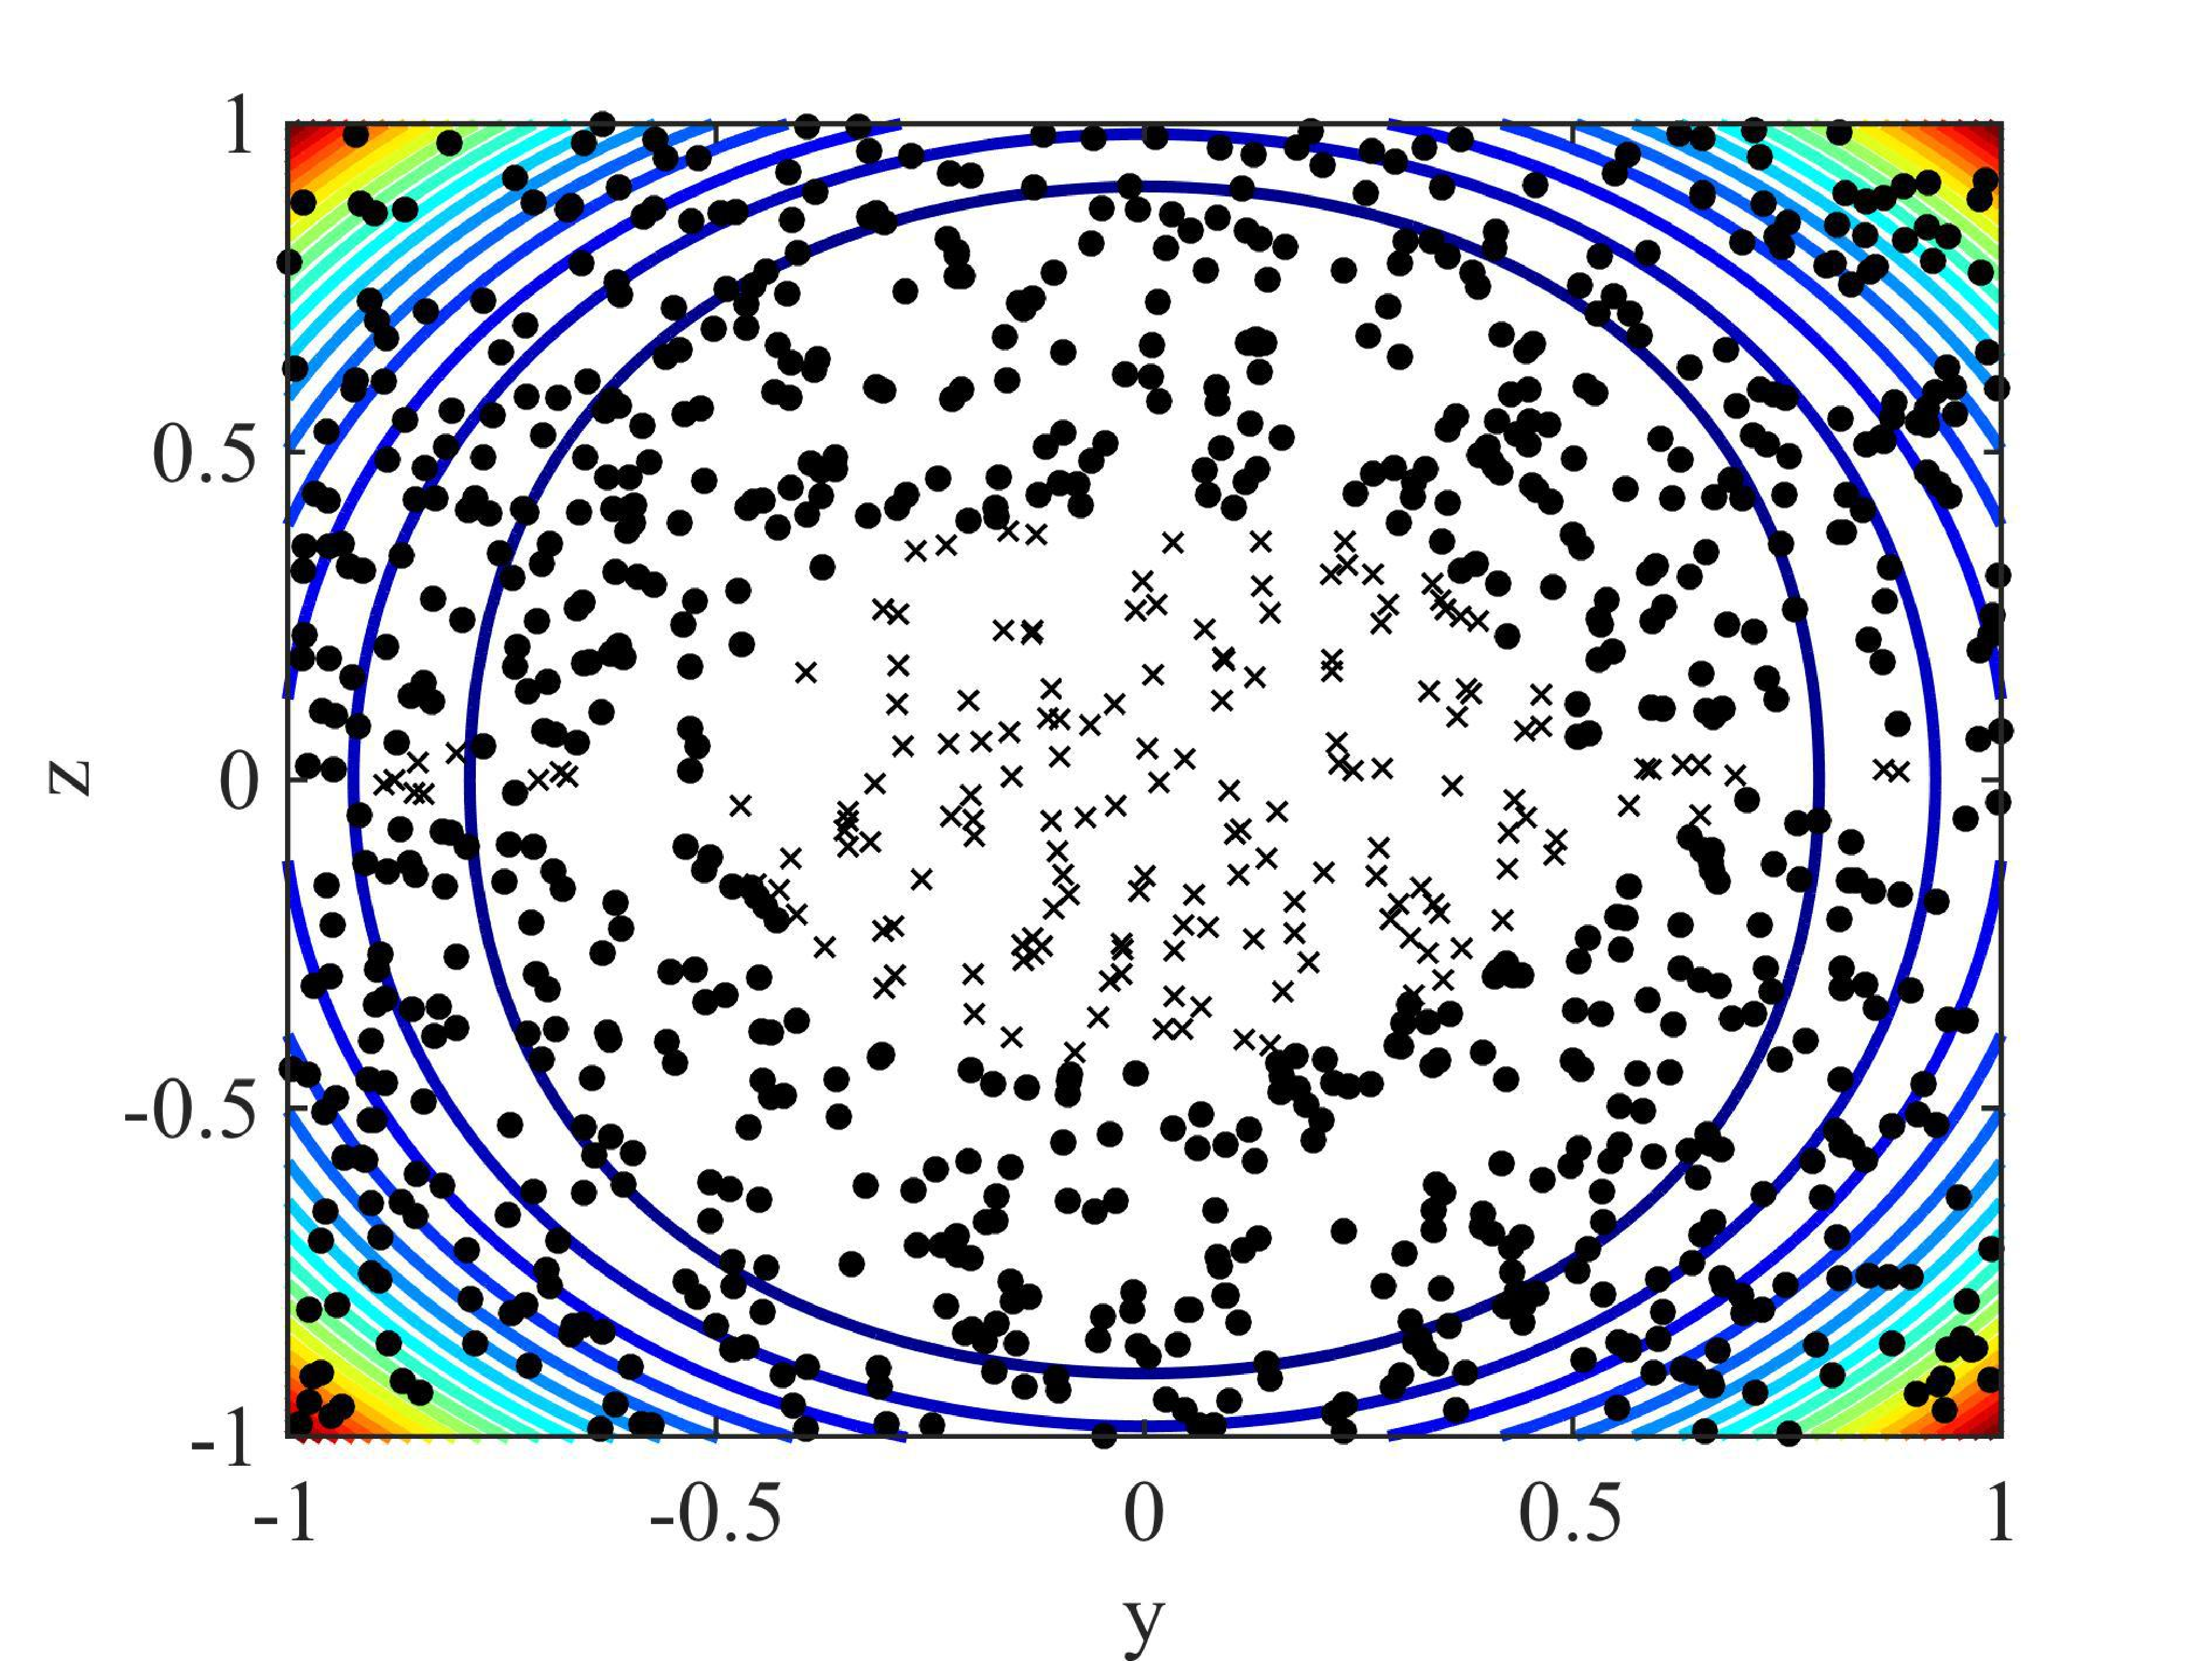
\includegraphics[width=0.45\textwidth]
   {figs/aniso_uniaxial_cartesian_random.pdf}
 } \subfigure[Stereographic]{
   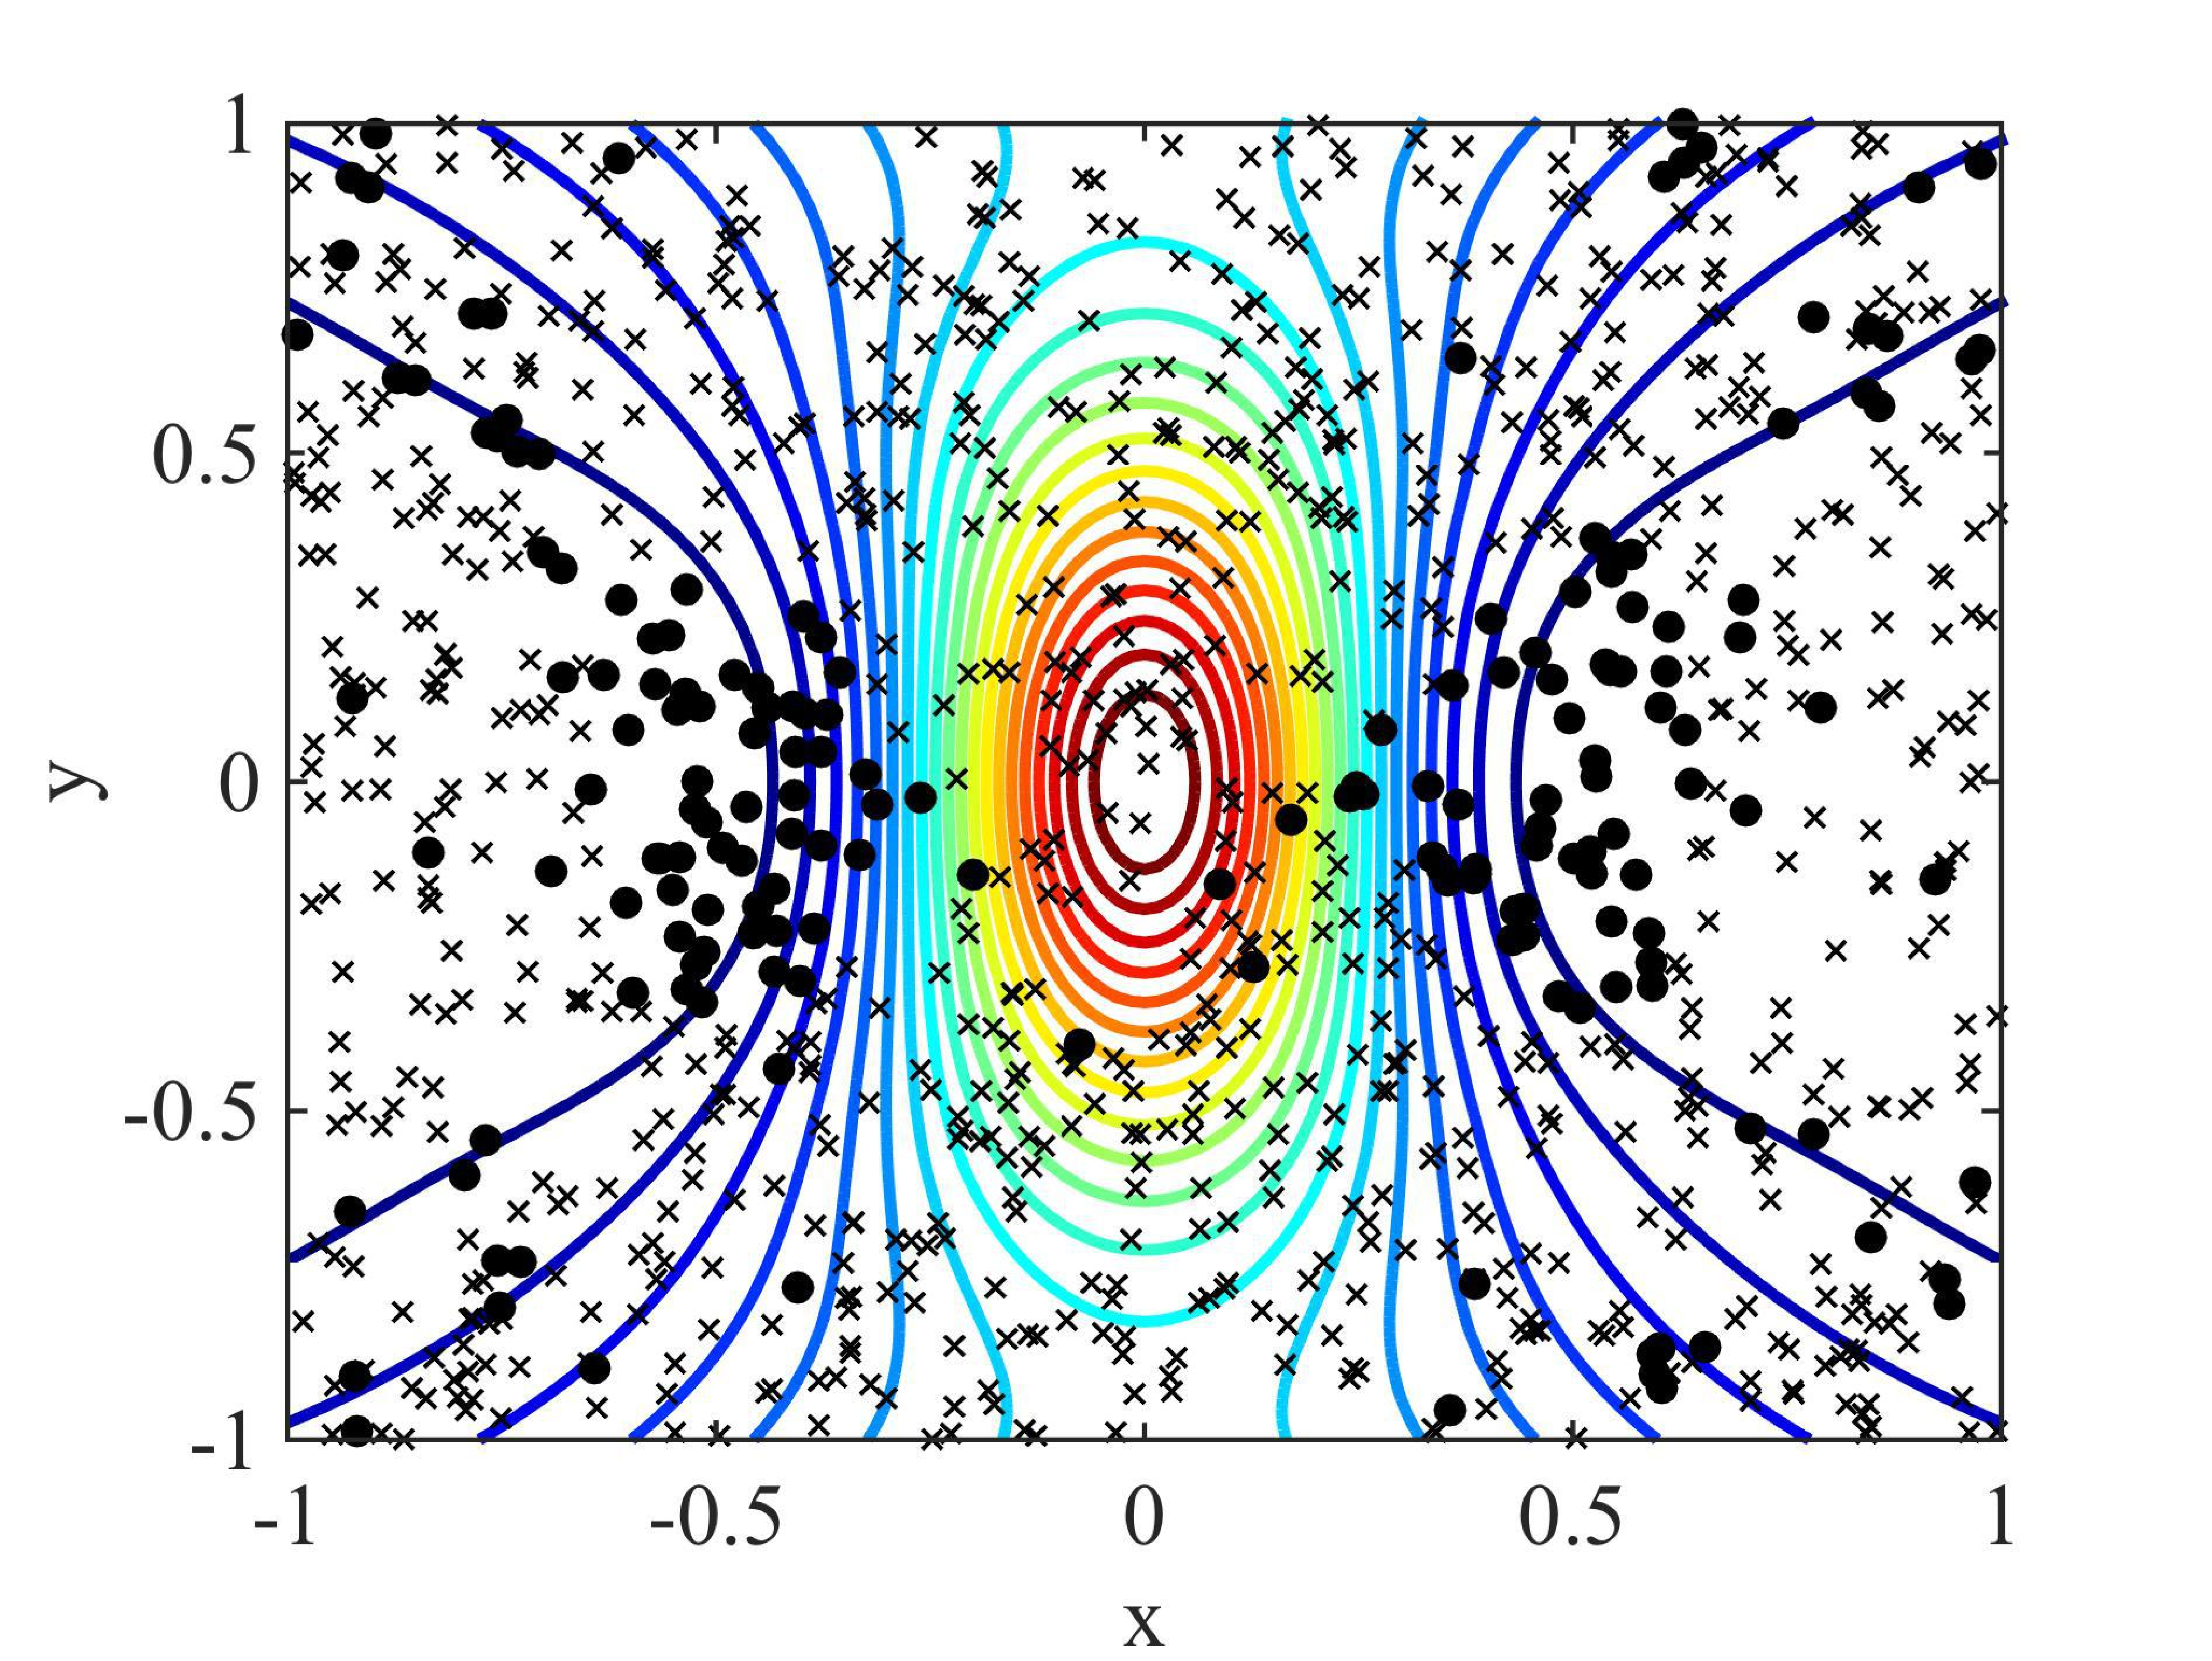
\includegraphics[width=0.45\textwidth]
   {figs/aniso_uniaxial_stereographic_random.pdf}
 } \subfigure[Tangent]{
   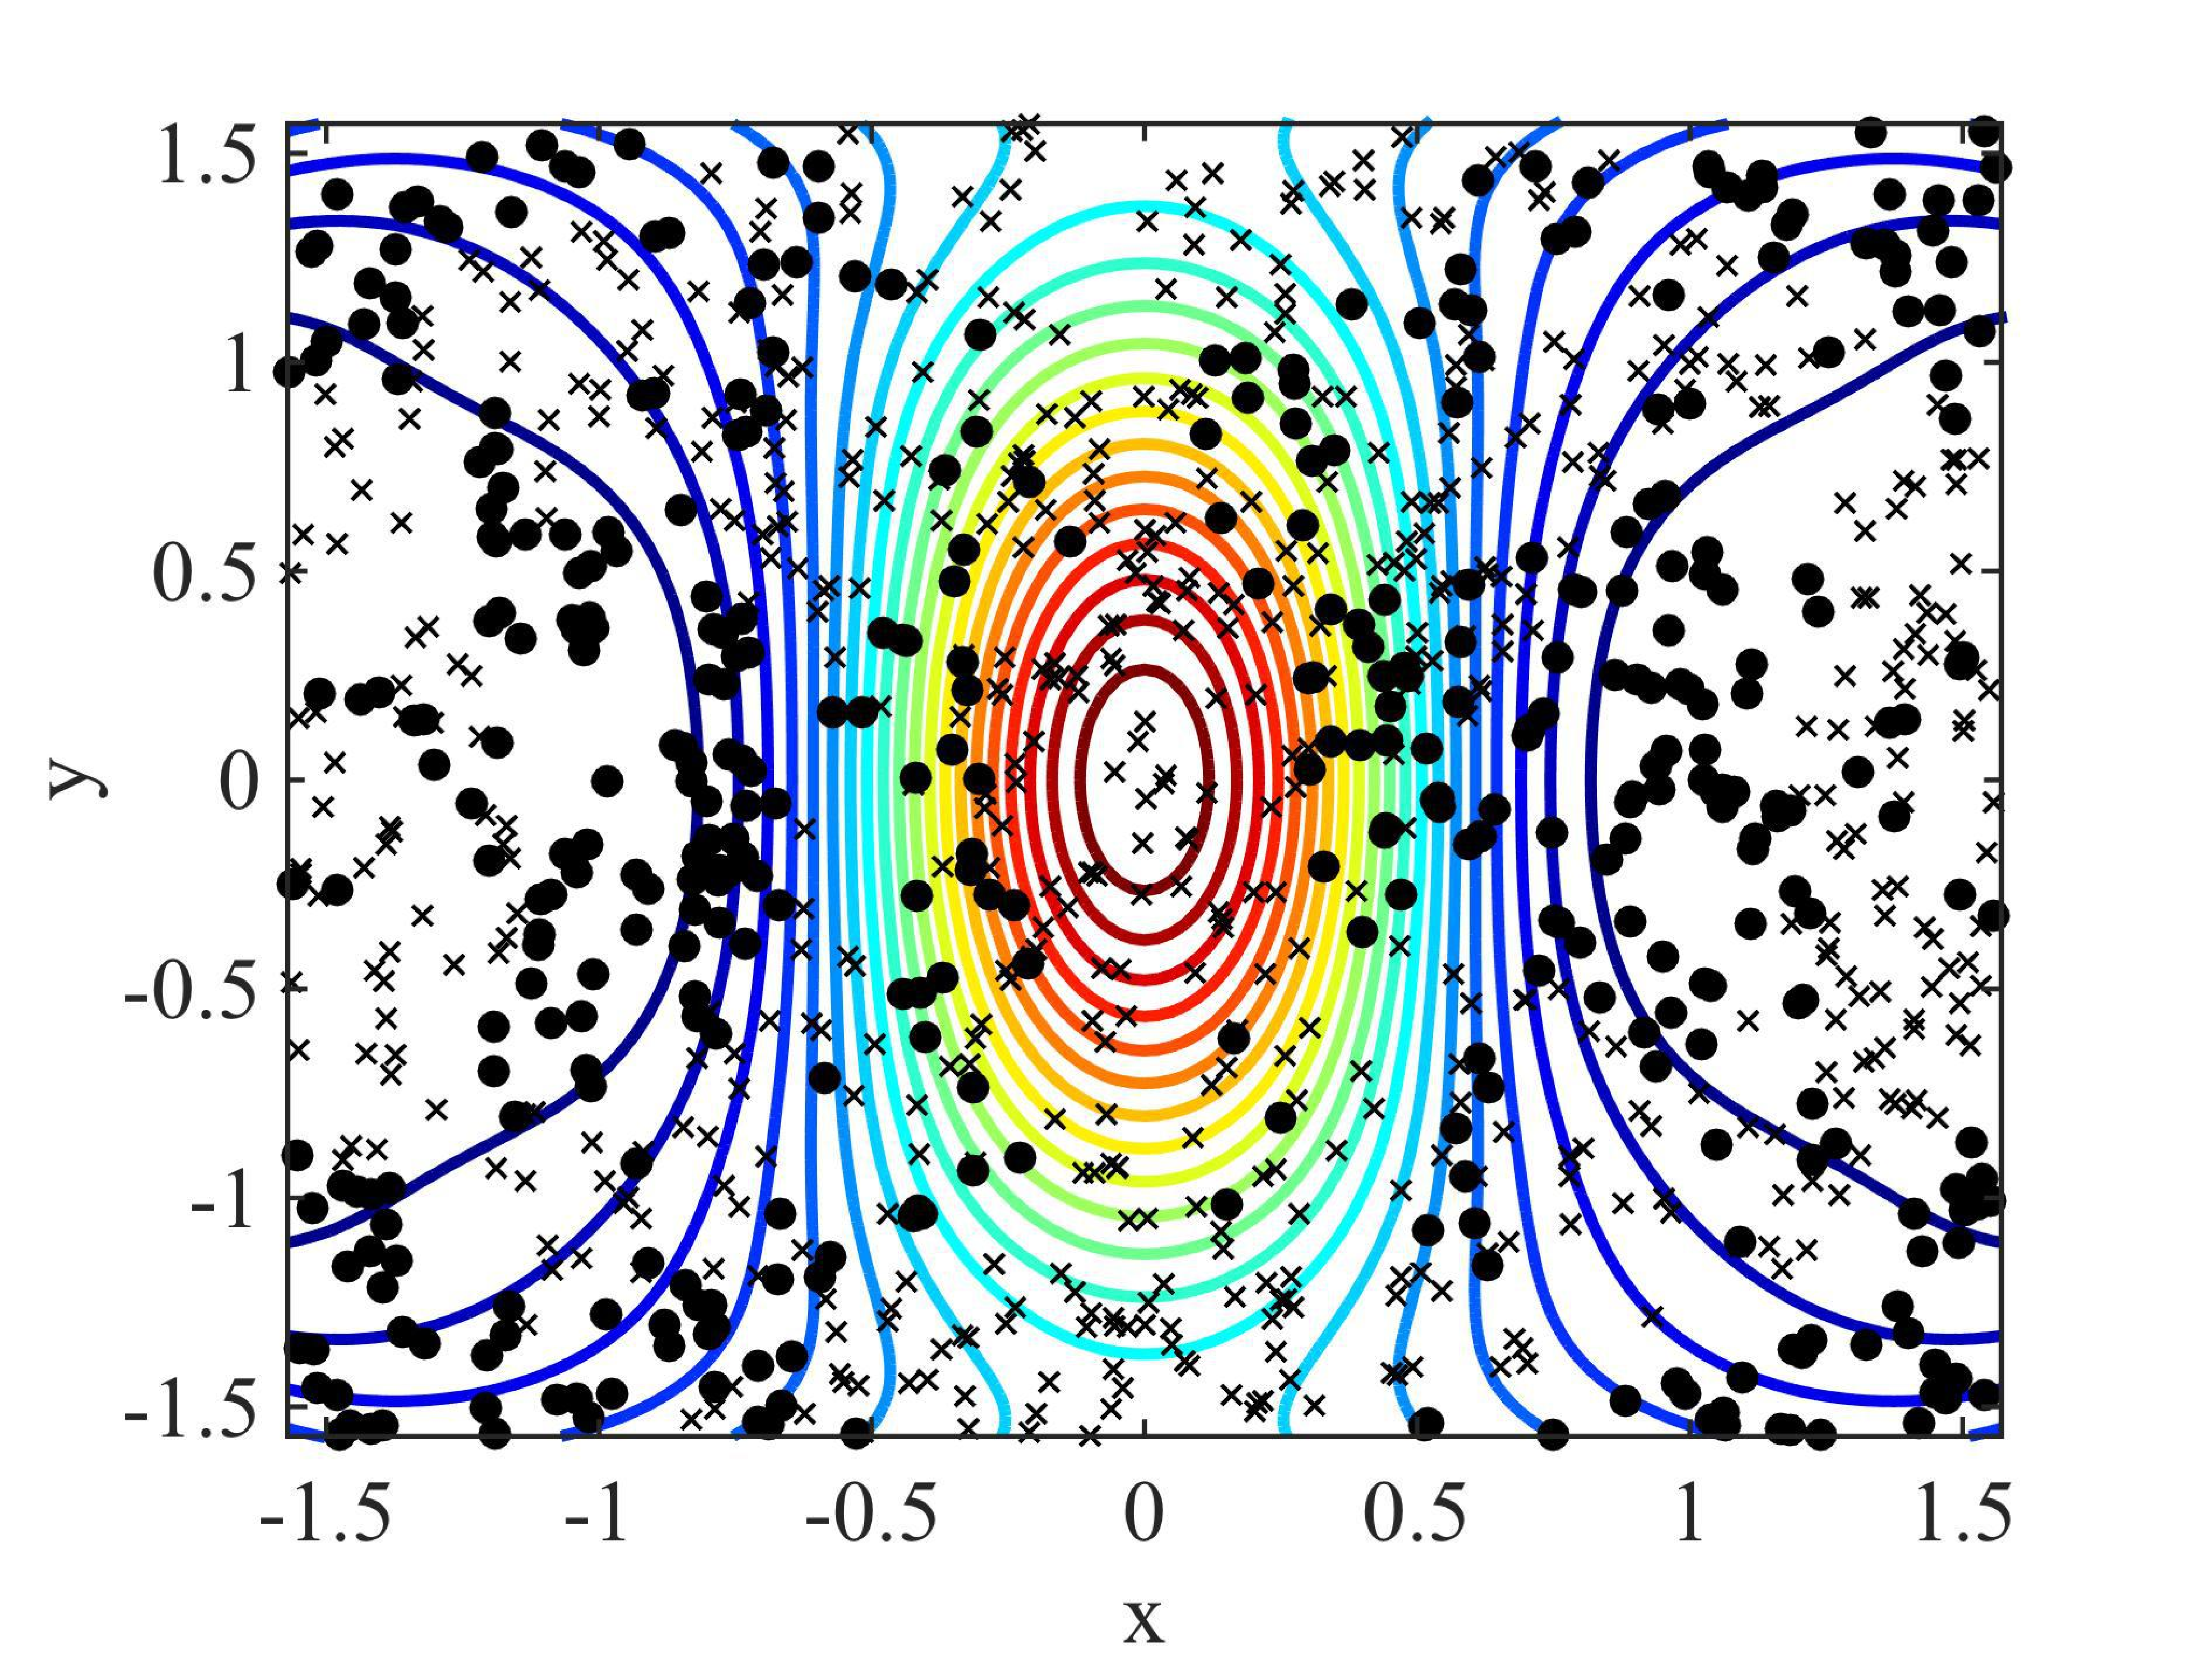
\includegraphics[width=0.45\textwidth]
   {figs/aniso_uniaxial_tangent_random.pdf}
 }
   \caption{Anisotropic finite deformation model: results of Newton 
   iterative solve with a single random initial point plotted on the 
   contour of determinant function at bifurcation. A solid circle 
   ($\bullet$) means the initial point leads to a success detection of 
   bifurcation and its directions. A cross ($\times$) means the Newton 
   iterative solve fails. A total of 1000 random trials are performed 
   for each parametrization.}
   \label{fig:aniso_uniaxial_robust}
 \end{figure}

Similar as in the case of the small deformation model example in 
Section \ref{subsec:isotropic}, the gradient-based optimization 
technique using Newton iterative solve is more likely to achieve 
convergence, even when the initial sweep is performed over a 
relatively coarse grid or without any initial sweep at all. The 
Cartesian parametrization is `optimal' in term of trade-off between 
computational efficiency and robustness. In a non-linear large-scale 
finite element simulation, this optimal trade-off between 
computational efficiency and robustness becomes critical. The 
Cartesian parametrization could provide a valuable tool in numerical 
bifurcation analysis. 

\section{Conclusion}

In this work, efficient and robust algorithms for numerical analysis 
of material instability are presented. A sweep-based algorithm 
followed by a Newton iterative method is adopted to solve the 
minimization problem of material instability. A new Cartesian 
parametrization for the normal vectors used to construct the acoustic 
tensor is proposed. The computational efficiency and robustness of the 
Cartesian parametrization is compared against other common and 
uncommon parametrizations of the acoustic tensor by means of numerical 
bifurcation analysis of an isotropic small deformation and an 
anisotropic large deformation damage model under different loading 
conditions. Summarizing results from numerical bifurcation analyses, 
it is found that:

\begin{enumerate}
\item[(1)] 
The parametrizations of the normal vector significantly affect the 
complexity of the objective function to be minimized, which in turn 
influences the computational efficiency and robustness of the 
algorithm. 

\item[(2)] 
The commonly used spherical parametrization is efficient provided 
that the initial sampling interval is fine enough and the initial 
guess is a good approximation to the minimum. 

\item[(3)] 
The stereographic and tangent parametrizations are the least 
robust, i.e., they are more likely to have convergence issues. The 
projective parametrization is much more expensive. 

\item[(4)] 
The Cartesian parametrization is the most robust one for all the 
material models and loading conditions tested. It is also 
computationally efficient. The Cartesian parametrization represent an 
optimal trade-off between computational efficiency and robustness and 
could provide a valuable tool for efficient and robust numerical 
analysis of material instability in large-scale finite element 
analysis. 
\end{enumerate}

%\bibliographystyle{plainnat}
\bibliographystyle{unsrtnat}
\bibliography{acpami}

\end{document}
